\documentclass[krantz1,ChapterTOCs]{krantz}
\usepackage{
	amsmath,
	amssymb,
	amsthm,
	chngcntr,
	comment,
	enumerate,
	etoolbox,
	fix-cm,
	float,
	graphicx,
	indentfirst,
	listings,
	mleftright,
	multicol,
	multirow,
	placeins,
	stix,
	subfig,
	threeparttable,
	totcount
}
\usepackage{graphicx}
\usepackage{epstopdf} % Load after graphiccx
%\usepackage[justification=centering]{caption}
\usepackage[figuresright]{rotating}
\usepackage[toc,page]{appendix}
\usepackage[autostyle]{csquotes}
\usepackage[obeyspaces,spaces]{url}
\hyphenation{con-sti-tu-tion-al}
\frenchspacing
\tolerance=5000
\setlength{\footnotesep}{0.7cm}
%\usepackage{fixltx2e}
%\usepackage{makeidx}


% ------------------------
% Warning Tolerances 
% ------------------------
\hfuzz=20pt
\vfuzz=20pt
\hbadness=2000
\vbadness=\maxdimen


% ------------------------
%  Font
% ------------------------
\usepackage[T1]{fontenc}
\usepackage[english]{babel}


% ------------------------
% Tikz & PGF
% ------------------------

% PGF
\usepackage{pgfplots}
\pgfplotsset{compat=newest}
\usepgfplotslibrary{fillbetween}

% Tikz
\usepackage{tikz}
\usetikzlibrary{shapes.misc,shadows,arrows,decorations.pathmorphing,patterns}


% ------------------------
% Comments (Remove Later)
% ------------------------
\usepackage{color}
\usepackage{todonotes}
\newcommand{\textnote}[1]{\textcolor{blue}{#1}}
\newcommand{\btodo}[1]{\todo[color=white]{\textcolor{blue}{#1}}}
\newcommand{\fancytodo}[1]{\todo[color=white,fancyline]{\textcolor{blue}{#1}}}


% ------------------------
% Commands
% ------------------------

% Letter Commands
\newcommand{\Tau}{\mathcal{T}}
\newcommand{\bm}[1]{\mbox{\boldmath{$#1$}}}
\newcommand{\bX}{\bm{X}}
\newcommand{\bY}{\bm{Y}}
\newcommand{\bZ}{\bm{Z}}

% Operators
\DeclareMathOperator{\var}{Var}
\DeclareMathOperator{\cov}{Cov}
\DeclareMathOperator{\corr}{Corr}
\DeclareMathOperator{\sgn}{sgn}
\DeclareMathOperator{\tr}{tr}
\DeclareMathOperator{\tvec}{vec}
\DeclareMathOperator{\tbvec}{Vec}
\DeclareMathOperator{\diag}{diag}
\DeclareMathOperator{\rank}{rank}
\DeclareMathOperator{\Prob}{Prob}
\DeclareMathOperator{\Ex}{E}

% Spacing Commands
\newcommand{\twomedskip}{\medbreak\medbreak}
\newcommand{\twoindent}{\indent\indent}

% Other Commands
\newcommand{\xqed}{\hfill \lower-0.3ex\hbox{$\triangleleft$}}
\newcommand{\zeropartnum}[1]{
	\ifcase\value{#1}\relax 0\else%
	\Roman{#1}\fi}% 
	\renewcommand{\thepart}{\zeropartnum{part}
}


% ------------------------
% Exercise Commands
% ------------------------
\newcounter{problem}
\newcommand{\prob}{
\stepcounter{problem} %
\noindent \theproblem. }
\counterwithin*{problem}{chapter}


% ------------------------
% Table Counter
% ------------------------
\counterwithin{table}{chapter}
\counterwithin{figure}{chapter}


% ------------------------
% Definitions, Theorems, Etc.
% ------------------------
\newtheoremstyle{custom}%   	% Name
  {}%                                     	% Space above
  {}%                                     	% Space below
  {}%                                     	% Body font
  {}%                                     	% Indent amount
  {\bfseries}%                            	% Theorem head font
  {.}%                                    	% Punctuation after theorem head
  { }%                                    	% Space after theorem head, ' ', or \newline
  {\thmname{#1}\thmnumber{ #2}\thmnote{ (#3)}}% 
  
\theoremstyle{plain}  
\newtheorem{prop}{Proposition}[section]
\newtheorem{lem}{Lemma}[section]
\newtheorem{cor}{Corollary}[section]

\theoremstyle{custom}
\newtheorem{ex}{Example}
\numberwithin{ex}{chapter}
\newtheorem{thm}{Theorem}[chapter]
\newtheorem{result}{Result}[chapter]
\counterwithout{result}{chapter}
\newtheorem{dfn}{Definition}

\theoremstyle{remark}
\newtheorem{rem}{Remark}[section] 
\numberwithin{equation}{chapter}


% ------------------------
% Title 
% ------------------------

% Title
\title{Algorithmic Trading and Quantitative Strategies \\ \vspace{3cm}  (Version: \today)} %This is a placeholder titlepage, it will not be final.

% Author
\author{\scalebox{1.5}{ Raja Velu\footnote{Department of Finance \hfill \newline \indent \indent Whitman School of Management \hfill \newline \indent \indent Syracuse University}, Maxence Hardy\footnote{Linear Quantitative Research \hfill \newline \indent \indent J.P. Morgan} and Daniel Nehren\footnote{Statistical Modeling \& Development \hfill \newline \indent \indent Barclays}}}


% ------------------------
% Document
% ------------------------
\begin{document}
\raggedbottom

% Front Matter
\frontmatter
\setcounter{page}{0}
% !TEX root = ../../book.tex
\pagenumbering{gobble}
{\bfseries\Huge Algorithmic Trading and \par Quantitative Strategies}

% Decorative Bar
\noindent\rule{\textwidth}{0.5pt} \par
\vspace{-0.3cm}\noindent\rule{0.25\textwidth}{4pt}


% Authors 
\vspace{0.5cm} 
\begin{minipage}{0.3\textwidth}
\large Raja Velu \par
{\scriptsize
Department of Finance \par
Whitman School of Management \par
Syracuse University \par
}
\end{minipage}%
\begin{minipage}{0.3\textwidth}
\large Maxence Hardy \par
{\scriptsize
eTrading Quantitative Research \par
J.P. Morgan \par
}
\end{minipage}%
\begin{minipage}{0.35\textwidth}
\large Daniel Nehren \par
{\scriptsize
Statistical Modeling \& Development \par 
Barclays \par
}
\end{minipage} \vfill

\begin{center} {\bfseries \Large To be Published by Chapman \& Hall/CRC Press} \end{center}

% Version
\vfill
\begin{center} \Huge {\bfseries (Version: \today)} \end{center}
% !TEX root = ../../book.tex

% Preface
\begin{center} {\Large\bfseries Preface} \end{center} \hspace*{\fill}
\addcontentsline{toc}{chapter}{Preface}

Algorithms have been around since the day trading has started. But they have gained importance with the advent of computers and the automation of trading. Efficiency in execution has taken center stage and with that, speed and instantaneous processing of asset related information have become important. In this book, we will focus on the methodology rooted in financial theory and demonstrate how relevant data---both in the high frequency and in the low frequency---can be meaningfully analyzed. The intention is to bring both the academics and the practitioners together. We strive to achieve what George Box (first author's teacher) once said: \par
        \begin{center}
        \begin{minipage}[t]{0.7\textwidth}
        	\raggedright
          	{\itshape``One important idea is that science is a means whereby learning is achieved, not by mere theoretical speculation on the one hand, nor by the undirected accumulation of practical facts on the other, but rather by a motivated iteration between theory and practice.''}
        \end{minipage} 
        \end{center}


We hope that we provide a framework for relevant inquiries on this topic. To quote Judea Pearl, \par
        \begin{center}
        \begin{minipage}[t]{0.7\textwidth}
        	\raggedright
          	{\itshape``You cannot answer a question that you cannot ask, and you cannot ask a question that you have no words for.''}
        \end{minipage} 
        \end{center}
The emphasis of this book, the readers will notice, is on data analysis with guidance from appropriate models. As C.R. Rao (first author's teacher) has aptly observed: \vspace{0.5\baselineskip}

\noindent All knowledge is, in final analysis, history. \par
\noindent All Sciences are, in the abstract, mathematics. \par
\noindent All judgements are, in the rationale, statistics. \twomedskip


This book gives an inside look into the current world of Electronic Trading and Quantitative Strategies. We address actual challenges by presenting intuitive and innovative ideas on how to approach them in the future. The subject is then augmented through a more formal treatment of the necessary quantitative methods with a targeted review of relevant academic literature. This dual approach is also reflective of the dynamics, typical of quants working on a trading floor where commercial needs, such as time to market, often supersede consideration of rigorous models in favor of intuitively simple approaches. 


Our unique approach in this book is to provide the reader with the hands-on tools. This book will be accompanied by a collection of practical Jupyter Notebooks where select methods are applied to real data. This will allow the reader to go beyond theory into the actual implementation, while familiarizing them with the libraries available. Wherever possible the charts and tables in the book can be generated directly from these notebooks and the data-sets provided bring further life to the treatment of the subject. We also add exercises to most of the chapters, so that the students can work through on their own. These exercises have been tested out by graduate students from Stanford and Singapore Management University. The notebooks as well as the data and the exercises are made  available on: \url{https://github.com/NehrenD/algo_trading_and_quant_strategies}. This site will be updated on a periodic basis. While reading and working through this book, the reader should be able to gain insight into how the field of Electronic Trading and Quantitative Strategies, one of the most active and exciting spaces in the world of finance, has evolved.


This book is divided into five parts. 

\begin{itemize}
\item Part~\ref{part:one} sets the stage. We narrate the history and evolution of Equity Trading and delve into a review of the current features of modern Market Structure. This gives the reader context on the business aspects of trading in order for them to understand why things work as they do. The next section will provide a brief high-level foundational overview of market microstructure which explains and models the dynamics of a trading venue heavily influenced by the core mechanism of how trading takes place: the price-time priority limit-order book with continuous double auction. This will set the stage for the introduction of a critical but elusive concept in trading: Liquidity.

\item Part~\ref{part:two} provides an overview of discrete time series models applied to equity trading. We will address univariate and multivariate time series models of both mean and variance of asset returns, and other associated quantities such as volume. While somewhat less used today because of high frequency trading, these models are important  as conceptual frameworks, and act as baselines for more advanced methods. We also cover some essential concepts in Point Processes as the actual trading data can come at irregular intervals. The last chapter of Part~I will present more advanced topics like State-Space Models and modern Machine Learning methods.

\item Part~\ref{part:three} dives into the broad topic of Quantitative Trading. Here we provide the reader with a toolkit to confidently approach the subject. Historical perspectives from Alpha generation to the art of backtesting are covered here. Since most quantitative strategies are portfolio-based, meaning that alphas are usually combined  and optimized over a basket of securities, we will briefly introduce the topic of Active Portfolio Management and Mean-Variance Optimization, and the more advanced topic of Dynamic Portfolio Selection. We conclude this section discussing a somewhat recent topic:  News and Sentiment Analytics. Our intent is to also remind the reader that the field is never ``complete'' as new approaches (such as this from behavioral finance) are embraced by practitioners once the data is available.

\item Part~\ref{part:four} covers Execution Algorithms, a sub-field of Quantitative Trading which has evolved separately from simple mechanical workflow tools, into a multi-billion dollar business. We begin by reviewing various approaches to modeling trade data, and then dive into the fundamental subject of Market Impact, a complex and least understood concept in finance. Having set the stage, the final section presents a review of the evolution and the current state of the art in Execution Algorithms.

\item Finally, Part~\ref{part:five} deals with some technical aspects of developing both quantitative trading strategies and execution algorithms. Trading has become a highly technological process that requires the integration of numerous technologies and systems,  ranging from market data feeds, to exchange connectivity, to low-latency networking and co-location, to back-office booking and reporting. Developing a modern and high performing trading platform requires thoughtful consideration and some compromise. In this part, we look at some important details in creating a full end-to-end technology stack for electronic trading. We also want to emphasize the critical but often ignored aspect of a successful trading business: Research Environment. \twomedskip
\end{itemize} 


%\addcontentsline{toc}{chapter}{Acknowledgements}
\noindent{\bfseries Acknowledgments:} The ideas for this book were planted ten years ago, while the first author, Raja Velu, was visiting the Statistics Department at Stanford at the invitation of Professor T.W. Anderson. Professor Tze-Leung Lai, who was in charge of the Financial Mathematics program, suggested initiating a course on Algorithmic Trading. This course was developed by the first author and the other authors, Daniel Nehren and Maxence Hardy, offered guest lectures to bring the practitioner's view to the classroom. This book in large part is the result of that interaction. We want to gratefully acknowledge the opportunity given by the Stanford's Statistics department and by Professors Lai and Anderson. 


We owe personal debt to many people for their invaluable comments and intellectual contribution to many sources from which the material for this book is drawn. The critical reviews by Professors Guofu Zhou and Ruey Tsay at various stages of writing are gratefully acknowledged. Colleagues from Syracuse University, Jan Ondrich, Ravi Shukla, David Weinbaum, Lai Xu, Suhasini Subba Rao from Texas A\&M, and Jeffrey Wurgler from New York University, all read through various versions of this book. Their comments have helped to improve its content and the presentation. Students who took the course at Stanford University, National University of Singapore and Singapore Management University and the teaching assistants were instrumental in shaping the structure of the book. In particular, we want to recognize the help of Balakumar Balasubramaniam, who offered extensive comments on an earlier version. On the intellectual side, we have drawn materials from the classic books by Tsay (2010); Box, Jenkins, Reinsel, Ljung (2015) on the methodology. Campbell, Lo and MacKinlay (1996) on finance; Friedman, Hastie and Tibshirani (2009) on statistical learning. In the tone and substance at times, we could not say better than what is already said in these classics and so the readers may notice some similarities.


We have relied heavily on the able assistance of Caleb McWhorter, who has put the book together with all the demands of his own graduate work. We want to thank our doctoral students, Kris Herman and Zhaoque Zhou (Chosen) for their help at various stages of the book. The joint work with them was useful to draw upon for content. As the focus of this book is on the use of real data, we relied upon several sources for help. We want to thank Professor Ravi Jagannathan for sharing his thoughts and data on pairs trading in Chapter~\ref{ch:stat_ts} and Kris Herman, whose notes on the Hawkes process are used in Chapter~\ref{chap:ch_trade_data_models}. The sentiment data used in Chapter~\ref{chap:ch_news_an} was provided by iSentium and thanks to Gautham Sastri. Scott Morris, William Dougan and Peter Layton at Blackthorne Inc, whose willingness to help on a short notice, on matters related to data and trading strategies is very much appreciated. We want to also acknowledge editorial help from Claire Harshberber and Alyson Nehren. 


Generous support was provided by Whitman School of Management and the Department of Finance for the production of the book. Raja Velu would like to thank former Dean Kenneth Kavajecz and Professors Ravi Shukla and Peter Koveos who serve(d) as department chairs and Professor Michel Benavoch, Associate Dean for Research, for their encouragement and support.


Last but not least the authors are grateful and humbled to have Adam Hogan provide the artwork for the book cover. The original piece specifically made for this book is a beautiful example of  Algorithmic Art representing trading intensity of the US stock universe on the various trading venues. We cannot think of a more fitting image for this book.  


Finally, no words will suffice for the love and support of our families. \vspace{3\baselineskip}


\noindent Raja Velu \par
\noindent Maxence Hardy \par
\noindent Daniel Nehren


\newpage


% ------------------------
% About the Authors
% ------------------------
%\addcontentsline{toc}{chapter}{About the Authors}
{\noindent\Large\bfseries About the Authors} \twomedskip

% Raja Velu
{\noindent\large\itshape Raja Velu} \medbreak

\noindent Raja Velu is a Professor of Finance and Business Analytics in the Whitman School of Management at Syracuse University. He obtained his Ph.D. in Business/Statistics from University of Wisconsin-Madison in 1983. He served as a marketing faculty at the University of Wisconsin-Whitewater from 1984 to 1998 before moving to Syracuse University. He was a Technical Architect at Yahoo! in the Sponsored Search Division and was a visiting scientist at IBM-Almaden, Microsoft Research, Google and JPMC. He has also held visiting positions at Stanford's Statistics Department from 2005 to 2016 and was a visiting faculty at Indian School of Business, National University of Singapore and Singapore Management University. His current research includes Modeling Big Chronological Data and Forecasting in High-Dimensional setting. He has published in leading journals such as Biometrika, Journal of Econometrics and Journal of Financial and Quantitative Analysis. \bigbreak

% Maxence Hardy
{\noindent\large\itshape Maxence Hardy} \medbreak

\noindent Maxence Hardy is a Managing Director and the Head of eTrading Quantitative Research for Equities and Futures at J.P. Morgan, based in New York. Mr. Hardy is responsible for the development of the algorithmic trading strategies and models underpinning the agency electronic execution products for the Equities and Futures divisions globally. Prior to this role, he was the Asia Pacific Head of eTrading and Systematic Trading Quantitative Research for three years, as well as Asia Pacific Head of Product for agency electronic trading, based in Hong Kong. Mr. Hardy joined J.P. Morgan in 2010 from Societe Generale where he was part of the algo team developing execution solutions for Program Trading. Mr. Hardy holds a master's degree in quantitative finance from the University Paris IX Dauphine in France. \bigbreak

% Daniel Nehren
{\noindent\large\itshape Daniel Nehren} \medbreak

\noindent Daniel Nehren is a Managing Director and the Head of Statistical Modelling and Development for Equities at Barclays. Based in New York, Mr. Nehren is responsible for the development of algorithmic trading product and model-based business logic for the Equities division globally. Mr. Nehren joined Barclays in 2018 from Citadel, where he was the head of Equity Execution. Mr. Nehren has over 16 years experience in the financial industry with a focus on global equity markets. Prior to Citadel, Mr. Nehren held roles at J.P. Morgan as the Global Head of Linear Quantitative Research, Deutsche Bank as the Director and Co-Head of Delta One Quantitative Products and Goldman Sachs as the Executive Director of Equity Strategy. Mr. Nehren holds a doctorate in electrical engineering from Politecnico Di Milano in Italy.


\newpage


% ------------------------
% Dedications
% ------------------------
%\addcontentsline{toc}{chapter}{Dedications}
%{\noindent\Large\bfseries Dedications} \twomedskip
Dedicated to\dots \twomedskip


\begin{minipage}[t]{0.8\textwidth}
	\raggedright
		Yasodha, without her love and support, this is not possible. \par
  	\raggedleft
  	R.V.
\end{minipage} \vspace{1cm}


\begin{minipage}[t]{0.8\textwidth}
	\raggedright
		Melissa, for her patience every step of the way, and her never ending support. \par
  	\raggedleft
  	M.H.
\end{minipage} \vspace{1cm}


\begin{minipage}[t]{0.8\textwidth}
	\raggedright
		Alyson, the muse, the patient partner, the inspiration for this work and the next. And the box is still not full. \par
  	\raggedleft
  	D.N.
\end{minipage} 

% Table of Contents
\cleardoublepage
\tableofcontents

% To-Do
%\listoftodos[Todo and Focus List]


% Main Matter
\mainmatter

% Context: Introduction and Overviews
\setcounter{part}{-1}
\part{Context: Introduction and Overview}
% !TEX root = ../../../book.tex

We provide a brief introduction to the book on the overall content and structure, and some basics of trading are covered. The initial part of Chapter~\ref{chap:ch_trading_fund} delves into a discussion of the market structure and trading from the practitioner's point of view. The terms used in this part, all can be traced back to academic literature; but the discussion is kept simple and direct. The data, which is central to all the analyses and inferences, is then introduced. The complexity of using data that can arise at irregular intervals can be better understood with an example illustrated here. Finally, the last part of this chapter contains a brief academic review of market microstructure---a topic about the mechanics of trading and how the trading can be influenced by various market designs.
% !TEX root = ../../book.tex
\chapter{Introduction}\label{chap:ch_intro}
\section{About This Book}

In recent years several books have been published  on the topics of Algorithmic Trading and Quantitative Strategies. Some books provide broad non-quantitative overviews of the subject while others are strictly academic, quantitative, treatments of one or more advanced theoretical topics. While these books hold a wealth of  information , we believe that none expose the reader to the complete picture, including the business aspects, the  practical challenges, and the tools needed for a quantitative researcher (aka Quant) to effectively operate.  This book strives to achieve exactly this goal. It is written by one academic that has studied and taught the methods of Quantitative Finance for over 20 years, and two senior quantitative practitioners with a combined 25$+$ years of experience in Electronic Trading who have worked (and still work) for some of the largest trading operations in the world. Bringing together these two diverse perspectives give the authors an opportunity to provide a unique,  practical, and integrated view of the field.


This book gives an inside look into the world of Electronic Trading and Quantitative Strategies addressing  actual challenges  often ignored by more academic treatments, evaluating past solutions, and presenting innovative ideas on how to approach them in the future. The subject is  then significantly deepened through a more formal mathematical treatment in order to provide the necessary quantitative methods as well as a targeted review of the relevant academic literature.


By construction (as well as by the obvious writing limitations of the authors) the book will thus present two very distinctive writing styles: one more high level, jargon ridden and conspicuously non rigorous, the other,  more formal and mathematical.  This dual approach is also reflective of the dynamics typical of quants working on a trading floor where commercial needs, time to market, and other practical considerations often supersede rigor and aesthetics of highly mathematical models, in favor of intuitively simple approaches. We hope that the reader will embrace this dual writing style.


Our approach to the more quantitative topics in this book is again, somewhat unique. In the spirit of providing the reader with the hands-on tools they need, this book will be accompanied by a collection of practical Jupyter Notebooks where select methods are applied to real data. This will allow the reader to go beyond theory into the actual implementation, while familiarizing them with the libraries available. Wherever possible the charts and tables in the book are generated directly from these notebooks and the data-sets provided bring further life to the treatment of the subject. We also add  exercises that the student can work through some of these problems on their own. The notebooks as well as the data and the exercises are made  available for free on: \url{https://github.com/NehrenD/algo_trading_book}.


While working through this book the reader should be able to create all the building blocks needed for a complete solution. They will also understand the context and challenges they will face in real life, and gain insight into how the field evolved in its sometimes dizzying complexity. We hope that the readers will enjoy this journey as much as the authors have enjoyed creating this ``guided tour'' into the workings of Electronic Trading and Quantitative Strategies, one of the most active and exciting spaces in the world of finance.

% How The Book is Structured
\section{How The Book is Structured}

This book is divided into five parts. 

\begin{itemize}
\item Part~0 sets the stage for our journey. After a whirlwind tour through the history and evolution of Equity Trading we will delve into a review of the current features of modern Market Structure in all its glory, chaos and (over-)complexity. This gives the reader context on the business aspects of trading in order for them to understand why things work as they do. The next section will provide a brief high-level overview of market microstructure which explains and models the dynamics of a trading venue  heavily influenced by the core mechanism in which trading usually takes place: the price-time priority limit-order book with continuous double auction. This will set the stage for the introduction of a critical but elusive concept in trading: Liquidity.

\item Part~I provides the foundational theory of stochastic processes and their connection to time series models applied to equity trading, and one of the core datasets in finance: Market Data. We will address univariate and multivariate time series models of both mean and variance of asset returns, and other associated quantities such as volume. While somewhat less used today, these models are important  as conceptual frameworks, and act as baselines for more advanced methods. The last chapter of Part 1 will present more advanced topics like State-Space Models and the applications of modern Machine Learning methods.

\item Part~II dives into the broad topic of Quantitative Trading. Here we provide the reader with a toolkit to confidently approach the subject. Historical perspectives to general approaches to Alpha generation to critical insights into the art of backtesting and its mine fields are covered here. Since most quantitative strategies are portfolio based, meaning that alphas are usually combined  and optimized over a basket of securities, we will briefly introduce the topic of Active Portfolio Management and Mean-Variance Optimization, and the more advanced topic of Dynamic Portfolio Selection. We conclude this section discussing a somewhat orthogonal topic:  News and Sentiment Analytics. Our intent is to also remind the reader that the field is never ``complete'' as new approaches (such as behavioral finance) and datasets become available and are embraced by practitioners.

\item Part~III is dedicated to Execution Algorithms, a sub-field of Quantitative Trading which has evolved separately from simple mechanical workflow tools, into a multi-billion dollar business. We begin from the ground up by reviewing various approaches to modeling trade data. We then do a deeper dive into the fundamental subject of Market Impact, one of the most complex and least understood concepts in the whole of finance. Having set the stage, the final section is dedicated to an in depth review of the evolution of and the current state of the art in Execution Algorithms.

\item Finally, Part~IV deals with several of the more technical aspects of developing both quantitative trading strategies and execution algorithms. Trading is a highly technological process that requires the integration of numerous technologies and systems,  ranging from market data feeds, to exchange connectivity, to low-latency networking and co-location, to back-office booking and reporting. Developing a modern and highly performing trading platform requires much consideration and compromise. In these chapters, we look at some of the most important details in creating a full end-to-end technology stack for electronic trading. We also dedicate a chapter to the critical but often ignore aspect of a successful trading business: The research environment.
\end{itemize} 
% !TEX root = ../../book.tex
%\hfill
%\par\vspace{\baselineskip}

\chapter{Execution Fundamentals}
\section{A Brief History of Stock Trading}
\section{Market Structure and Trading Venues: A Review}
\section{The Mechanics of trading: The Limit Order Book}
\subsection{How Double Auction Markets Work}
\subsubsection{Order Types}
\subsubsection{The Open Auction}
\subsubsection{Continuous Trading}
\subsubsection{The Closing Auction}
\subsection{Market Data}
\subsubsection{Reference Data}
\subsubsection{Daily Statistics}
\subsubsection{Level 1: Trade, Quotes, BBO and NBBO}
\subsubsection{Level 2: Market Depth}
\subsubsection{Level 3: Orders}

\section{The Dynamics of Trading: Market Micro-structure}
\section{Execution and its components}
\subsection{Benchmarks}
\subsection{Scheduling}
\subsection{Order Placement}
\subsection{Order Routing}



% Foundations: Basic Models and Empirics
\part{Foundations: Basic Models and Empirics}
% !TEX root = ../../../book.tex

In Part~I, our goal is to provide a review of some basic and some advanced statistical methodologies that are useful for developing trading algorithms. We begin with time series models (in Chapter~\ref{ch:ch_uvts}) for univariate data and provide a broad discussion of autoregressive, moving average models---from model identification, estimation, inference to model diagnostics. The stock price and return data exhibit some unique features and so we identify certain stylized facts regarding their behavior that have been empirically confirmed; this work will greatly help to discern any anomalies as and when they arise, as these anomalies generally indicate deviation from efficient market hypothesis. Although for modeling price and return data, only lower order models are needed, increasingly other trading features such as volume, volatility are being used in developing trading strategies. In particular,  predicting future volume flow to determine when to enter the market, requires the use of higher order models. Wherever possible we illustrate the methodology with examples and provide codes for computing, making the data accessible to the reader. 


This chapter is followed by methodologies for multiple time series data and the discussion in Chapter~\ref{ch:ch_mvts} is useful from pairs trading to portfolio optimization. The last chapter (Chapter~\ref{ch:ch_advanced}) in Part~I contains advanced topics such as theory of point processes as trading takes place on a continual basis. Understanding the market microstructure is essential for deciding about the entry to and exit from the market. This chapter also contains other modern topics such as machine learning and artificial intelligence. 


A reader with a strong statistics background can afford to skip some sections but we recommended to peruse these chapters as they contain discussions on topics that need further research work. In presenting the methodologies here, we keep the discussion lucid but immensely relevant to the main theme of this book---understanding the market behavior and developing effective trading strategies. 
% !TEX root = ../../book.tex
\chapter{Univariate Time Series Models\label{ch:ch_uvts}} \label{in:tsm1}

With the advent of electronic trading a vast amount of data on orders is now recorded and is available to traders to make real-time decisions. The Trades and Quotes (TAQ)\label{in:taq1} data on time-stamped sequence of trades with the updates on the price and depth of the best bid and ask quotes was used by researchers and traders initially. This was later expanded to the so-called Level~II data, with time-stamped sequence of trades and quotes for the top 5 levels of the order book. Both TAQ and Level~II data still do not provide the complete story of the buy and sell sides. With Level~III data now available, we can obtain time-stamped sequence of all events that occur (with the exception of the information on hidden orders), resulting in a quite voluminous, but irregularly spaced, data set. We take a broad view that for making strategic decisions to enter and exit the market, the trader needs to take an aggregate view of the trading activities, but that for the optimal execution of the strategies the trader needs to understand the market microstructure that relates to the actual process of trading. With the increased speed of decisions in an HFT world, the difference between the two steps, strategic and execution decisions, may be blurred but the aggregation process can help to look beyond trading frictions. In Section~\ref{sec:tradesandquotes}, we discuss the Trades and Quotes data and aggregation issues. In Section~\ref{sec:trad_dec_stfd}, we define trading algorithms that depend on prediction of short-term price movement.


The price movement, whether it is due to pure market friction or due to information related to a stock, is captured through a drift term in the random walk model that needs to be carefully monitored. Because time series models for discrete time units are still widely used by traders in the form of aggregated price-bars, we focus on these methods in Sections~\ref{sec:model_mean} to Section~\ref{sec:sty_mod_var}. We broadly classify these methods into modeling the mean (return) and into modeling the variance (volatility). As these techniques are well-documented and can be found elsewhere in the literature, we only present a brief but relevant overview. The established facts about the stock returns and variances are reviewed along with the methodology as these will provide expected benchmarks; successful algorithms as one would notice, generally exploit the deviations from these benchmarks.



% Trades and Quotes Data and their Aggregation
\section{Trades and Quotes Data and their Aggregation: From Point Processes to Discrete Time Series\label{sec:tradesandquotes}}

In its simplest form, the trading activities through an exchange that opens at 9:30~a.m. and closes at 4~p.m. can be described by a sequence of time stamps (``ticks'') $t_0 < t_1 < \cdots < t_n$ and the ``marks'' $y_i$ at time $t_i$, in which $t_0$ denotes 9:30~a.m. and after and $t_n$ denotes the time of the last trade that occurs before or at 4~p.m. The marks $y_i$ can be price, volume of an order placed on either the buy or sell side of the book and in general can represent the characteristics of the order book at the time of $i$th activity (see Figure~\ref{fig:tradeactline}). The events with the marks associated with the ticks can be described mathematically as a marked point process. But our goal here is to first show how these data points can be aggregated over regularly spaced time intervals and how methods for linear homogeneous time series can be used to analyze the aggregated data. Some tools that are relevant for the analysis of point processes will be presented in Chapter~\ref{ch:ch_advanced}. \label{in:disc_time_unit1} \label{in:level3dat2}
	\begin{figure}[!ht]
	\centering
	\begin{tikzpicture}
	\draw[line width=0.08cm] (-5,0) -- (5,0);
	
	\draw[line width= 0.05cm] (-5,-0.3) -- (-5,0.3);
	
	\draw[line width = 0.05cm] (-4,-0.3) -- (-4,0.3);
	\draw[line width = 0.05cm] (-3,-0.3) -- (-3,0.3);
	\draw[line width = 0.05cm] (-2,-0.3) -- (-2,0.3);
	
	\draw[line width=0.05cm] (5,-0.3) -- (5,0.3);
	
	\node at (-5.1,-0.6) {9:30 a.m.};
	\node at (4.9,-0.6) {4:00 p.m.};
	
	\node at (-3.95,-0.65) {$t_1$};
	\node at (-2.95,-0.65) {$t_2$};
	\node at (-1.95,-0.65) {$t_3$};
	
	\node at (-3.95,-1.2) {$y_1$};
	\node at (-2.95,-1.2) {$y_2$};
	\node at (-1.95,-1.2) {$y_3$};
	
	\foreach \xcoord in {-1.5,-1.0,...,3.8} 
	{
	\draw[fill] (\xcoord,-0.95) circle (0.03cm);
	}
	\end{tikzpicture}
	\caption{Trading Activities. \label{fig:tradeactline}}
	\end{figure}


The typical Level~III data for CISCO on a single day in 2011 is given below in Table~\ref{tab:CISCO}. This outlay in Table~\ref{tab:CISCO} points to various issues that need to be addressed in processing this type of data. The order numbers are only unique during the lifetime of the order but can be reassigned at a later time. Several activities such as submissions, cancellation or modification of an order, all can take place at the same time stamp. Hidden orders are revealed only when they are executed and as such do not have visible order numbers.\label{in:hidden1} Full cancellation quantity and price information should be traced back to the submission time. To summarize, at any given point in time using the data described in Table~\ref{tab:CISCO}, the full limit order book that essentially records where each order is in the queue, can be constructed and thus providing the activity time and the associated marks. These and other characteristics of the limit order book (superbook---if we collate this information from all exchanges) will be taken up in a later chapter, but the focus here is on constructing discrete time series data from this point process data. 
	\begin{table}[!ht]
   	\centering
   	\caption{CISCO--Trade Data \label{tab:CISCO}}
   	\hspace{-1cm}\begin{tabular}{cccccc} 
	Timestamp & Order Number & Event & Quantity & Price & Exchange \\ \hline
	$\vdots$ & $\vdots$ & $\vdots$ & $\vdots$ & $\vdots$ & $\vdots$ \\
	34561915 & 4254917 & D & 0 & 0 & J \\
	34561915 & 4253917 & B & 200 & 20.55 & J \\
	$\vdots$ & $\vdots$ & $\vdots$ & $\vdots$ & $\vdots$ & $\vdots$ \\
	34561923 & 13056048 & S & 200 & 20.58 & Z \\
	$\vdots$ & $\vdots$ & $\vdots$ & $\vdots$ & $\vdots$ & $\vdots$ \\
	34573369 & 13255731 & C & 98 & 0 & Q \\
	$\vdots$ & $\vdots$ & $\vdots$ & $\vdots$ & $\vdots$ & $\vdots$ \\
	34577331 & 6225085 & E & 300 & 0 & K \\
	$\vdots$ & $\vdots$ & $\vdots$ & $\vdots$ & $\vdots$ & $\vdots$ \\
	34577338 & 6225085 & F & 0 & 0 & K \\
	$\vdots$ & $\vdots$ & $\vdots$ & $\vdots$ & $\vdots$ & $\vdots$ \\
	34573379 & 2030057 & S & 100 & 20.77 & K \\
	$\vdots$ & $\vdots$ & $\vdots$ & $\vdots$ & $\vdots$ & $\vdots$ \\
	34573382 & NA & T & 1700 & 20.37 & P \\
	$\vdots$ & $\vdots$ & $\vdots$ & $\vdots$ & $\vdots$ & $\vdots$ 
   	\end{tabular}
	\begin{minipage}[t]{1\textwidth}
	\small{*Time-stamp is the time since midnight; Event: B: submission of LO on Buy side; S: submission of LO on Sell side; T: Full execution of a hidden LO; F: full execution of a visible LO; E: partial execution of a LO; D: full cancellation of a LO; C: partial cancellation of a LO; Exchange: Q-NASDAQ; J-EDGE-A; Z-BATS-Z; K-EDGE-K; P-ARCA; etc}
	\end{minipage}
	\end{table}


To illustrate the aggregation methods, we will initially focus on price of the stock, $P_t$, and the associated volume $V_{t}$. Two types of aggregation methods are proposed in the literature. One when the time span $T$ for the Exchange hours (9:30~a.m.--4:00~p.m.) is divided into `$K$' intervals (Clock Time) so that the regularly spaced intervals are of size $\Delta t = T/K$. The other method will do aggregation when there is a change in a marker, such as price (Volume Time). Here we focus on the first method. Various summary measures within each period $((i - 1)\Delta t, i\Delta t)$ where $i = 0,1,\ldots,K$ can be computed;
        \begin{itemize}
        \item number of transactions: `$n_i$'
        \item Average price: $\overline{P}_i = \sum P_{t_j}/n_i$
        \item Volume Weighted Average Price: $\overline{P}_{wi} = \sum V_{t_j} P_{t_j}/ \sum V_{t_j}$
        \item Average duration between transactions: $\overline{d}_i = \sum_{j\in ((i-1)\Delta t,i\Delta t) }(t_j - t_{j-1})/n_i$
        \item Mid-Price: $(\text{Best bid}_i+\text{Best ask}_i)/ 2$
        \end{itemize}


The typical daily data (also-called price bars) that is available from popular online sources provide information on opening, closing, high and low prices along with the volume. This type of aggregation can also be done for shorter duration, such as one or five minutes, resulting in smoothed data that can cancel out short term market frictions and yet capture the price variations that may be due to information. 


It is possible that for infrequently traded stocks, some time intervals may not contain any trading activity. For heavily traded stocks, the duration can be very small and thus may not provide any consequential information. We will discuss this further in Chapter~\ref{ch:ch_advanced}. To begin with, we present the analysis for data aggregated over fixed time intervals. Depending on the size of the interval, the data can be called low frequency or high frequency but the time series methods that are discussed in this chapter apply to \emph{all} aggregated data.



% Trading Decisions as Short-Term Forecast Decisions
\section{Trading Decisions as Short-Term Forecast Decisions \label{sec:trad_dec_stfd}} 

Most trading decisions generally involve the following considerations
        \begin{itemize}
        \item How much to trade?
        \item When to trade, i.e. when to enter and when to exit?
        \item How to trade? How fast? What is the objective? What are the benchmarks?
        \end{itemize}
Answers to these questions involve in some way predicting the market movement and in particular the future (short-term and long-term) price of assets. In the short term it is possible that prices have a tendency to `trend' or exhibit `momentum' but in the long run, prices have a tendency to `mean-revert' as the information about the asset gets incorporated into the price. 


Let $p_{it}= \ln P_{it}$ denote the price of the $i$th asset at time $t$ and let $p_t = (p_{1t}, p_{2t}, \ldots, p_{nt})$ denote the price vector for `$n$' assets. Let $y_{it}$ denote a vector of characteristics, e.g. volume of transactions, price volatility, number of transactions and the intensity of trading as captured by the average duration between transactions, etc of the $i$th asset at time $t$. These quantities are aggregated from high frequency data of the type given in Table~\ref{tab:CISCO} and illustrated in Figure~\ref{fig:tradeactline} to be used as the characteristics associated with the price changes. In addition, we can also consider $r$ factors $f_t = (f_{1t}, f_{2t}, \ldots, f_{rt})$ that may include market and industry factors as well as asset characteristics such as market capitalization, book-to-market ratio etc. The trading rules can be broadly grouped as follows:
        \begin{itemize}
        \item[A.] Statistical Arbitrage Rules: $\Ex(p_{i,t+1}\,|\,p_{i,t},p_{i,t-1},\ldots,y_{i,t},y_{i,t-1},\ldots)$
        \begin{itemize}
        \item[$\bullet$] Predicting the price of $i$th stock at t+1 based on the past trading information; this is sometimes labelled as time series momentum.
        \end{itemize}
        \item[B.] Momentum: $\Ex(p_{t+1}\,|\,p_{t},p_{t-1},\ldots,y_{t},y_{t-1},\ldots)$
        \begin{itemize}
        \item[$\bullet$] Predicting the cross-sectional momentum of a subset of stocks based on their past trading characteristics. This is not only useful for portfolio formation and rebalancing, also for pairs trading which is based on tracking two stocks simultaneously so that their price divergence can be exploited. 
        \end{itemize}
        \item[C.] Fair Value: $\Ex(p_{t+1}\,|\,p_{t},p_{t-1},\ldots,y_{t},y_{t-1},\ldots,f_t,f_{t-1},\ldots)$
        \begin{itemize}
        \item[$\bullet$] Predicting the price using all relevant quantities. The factors normally include market and Fama-French factors. Many of these factors are at a more macro level than the time scale considered for the price prediction, but nevertheless could be useful, as explained in Chapter~\ref{ch:ch_mvts}.
        \end{itemize}
        \end{itemize}
\noindent Thus the price (or alternatively, return) and volatility (or squared return) prediction can be formulated as a time series prediction problem and common tools such as autocorrelations and partial autocorrelations can be used to build autoregressive and ARCH models that are shown to have some predictive power. 


Predicting stock market behavior has been studied extensively starting in the early 20th century. Cowles (1933, 1944)~\cite{cow1,cow2} evaluated the performance of the stock market forecasters. Analyzing the performance of several financial services that made some 7500 recommendations on common stocks over a period, January 1, 1925 to July 1, 1952, they pointed out the record was worse than the performance of average common stock by 1.43\% annually. Thus `buy-and-hold' strategy out-performed the stock picking strategies of those days. In fact, a much harsher assessment is made: ``A review of the various statistical tests, applied to the records for this period, of these 24 forecasters, indicates that the most successful records are little, if any, better than what might be expected to result from pure chance. There is some evidence, on the other hand, to indicate that the least successful records are worse than what could reasonably be attributed to chance.'' Many of these comments are still valid and have stood the test of the time. Yet, we will demonstrate in this book that there are opportunities for statistical arbitrage. The key being to have access to relevant information and using appropriate techniques to exploit the information in a timely manner. 



% Stochastic Processes
\section{Stochastic Processes: Some Properties\label{sec:stoc_proc}}

Formally, a discrete time series or stochastic process $Y_1, Y_2, \ldots, Y_T$ is a sequence of random variables (r.v.'s) possessing a joint probability distribution. A particular sequence of observations of the stochastic process $\{ Y_t, t=1, \ldots,  \, T\}$ is known as a realization of the process. In general, determining the properties and identifying the probability structure which generated the observed time series are of interest. We do not attempt to study the joint distribution of $Y_1, Y_2, \ldots, \, Y_T$ directly, as it is too complicated for large $T$, but we study the probabilistic mechanism which generates the process sequentially through time, and from this we want to derive the conditional distribution of future observations for purposes of prediction.


The means, variances, and covariances are useful summary descriptions of the stochastic process $\{ Y_t, t=1,\ldots,\,T \}$, but it is not possible to estimate the unknown parameters (means, variances, and covariances) from a single realization of $T$ observations if these quantities vary with `$t$'. We impose some additional structure on the joint distribution of the process in order to substantially reduce the number of unknown parameters. The concept of stationarity of a process serves as a realistic assumption for many types of time series. Stationarity is motivated by the fact that for many time series in practice, segments of the series may behave similarly. \twomedskip


\noindent\textbf{Stationarity} \twomedskip


A time series $\{Y_t \}$ is said to be stationary if for every integer $m$, the set of variables $Y_{t_1}, Y_{t_2}, \ldots, \, Y_{t_m}$ depend only on the distance between the times $t_1, t_2, \ldots, t_m$, rather than on their actual values.  So a stationary process $\{Y_t \}$ tends to behave in a homogeneous manner as it moves through time. The means and variances of the $Y_t$ are the same for all $t$, that is, $\Ex(Y_t) = \mu$ and  $\var(Y_t)= \sigma^2$ are constant, for all $t$. So we may express the autocovariance function as 
	\begin{equation} \label{eqn:2gammas}
	\gamma(s)= \cov(Y_t,Y_{t - s})= \Ex[(Y_t - \mu)(Y_{t - s} - \mu)], \text{ for all } s= 0, \pm 1, \ldots
	\end{equation}
Note that by this notation, $\gamma(0) = \Ex[(Y_t - \mu)^2] = \var(Y_t)$. Also, the \emph{autocorrelation function} of the stationary process may be expressed
        	\begin{equation} \label{eqn:2rhos}
	\rho(s)= \corr(Y_t,Y_{t - s})= \dfrac{\cov(Y_t,Y_{t - s})}{\big( \var(Y_t) \var(Y_{t-s}) \big)^{1/2}} = \dfrac{\gamma(s)}{\gamma(0)},  \quad  s= 0, \pm 1, \ldots
	\end{equation}
$\rho(s)$ will be referred to as the autocorrelation of the process at lag $s$. The autocorrelation function (ACF), $\rho(s)$ of a stationary process $\{Y_t\}$ is an important tool in describing the characteristics of the process, because it is a convenient summary of the correlation structure of the process over different time lags.  \twomedskip


\noindent \textbf{Examples of Stationary Stochastic Processes} \twomedskip


Now we present some select models, as examples, that tend to be the most useful in financial applications. The properties of these models would become relevant as we look at data. 


\begin{ex}[White Noise] \label{ex:whitenoise} Let $\epsilon_0, \epsilon_1, \epsilon_2, \ldots$ be a sequence of independent random variables defined on the discrete time points $0,1, 2, \ldots$, with mean $\Ex(\epsilon_{t})= 0$ and variance $\Ex(\epsilon_{t}^2)= \sigma^2$, for all $t$. Set $Y_t = \mu + \epsilon_t, \, t= 0, 1, 2, \ldots$. Then $\Ex(Y_t)= \mu$ for all $t$, and since independence implies that the random variables are uncorrelated, we have $\cov(Y_t,Y_{t-s})= \var(Y_t)= \sigma^2$ if $s=0$ and $\cov(Y_t,Y_{t-s})= 0$ if $s \neq 0$. Thus the process is stationary. Such a process is referred to as purely random process or a \emph{white noise process}, and is the foundation for the construction of many other processes of interest. \xqed
\end{ex}


\begin{ex}[Moving Average] \label{ex:movingaverage} Let $\{ \epsilon_t \}$ be independent r.v.'s as in Example~\ref{ex:whitenoise}, and define a new process $\{ Y_t \}$ by
	\[
	Y_t = \mu + \epsilon_t + \epsilon_{t-1}, \qquad t=0, 1, 2, \ldots,
	\]
where $\mu$ is a constant.  Then $\Ex(Y_t)= \mu$, for all $t$, and
	\[
	\cov(Y_t,Y_{t-s})= \gamma(s) =
	\begin{cases}
	2 \sigma^2 & \text{if } s= 0 \\
	\sigma^2 & \text{if } s= 1 \\
	0 & \text{if } s > 1
	\end{cases}
	\]
which depends only on the time lag $1$ and not on $t$.  Hence the process $\{ Y_t \}$ is stationary with ACF $\rho(s)= \gamma(s)/\gamma(0)$ such that $\rho(0)= 1$, $\rho(1)= 1/2$ and $\rho(s)= 0$ for $\lvert s \rvert > 1$.
 
	\begin{sidewaysfigure}[hbp]
	%\centering
                \subfloat[Figure 1a]
                        [Time series plot of $0.5 + \epsilon_t$]
                        {
                        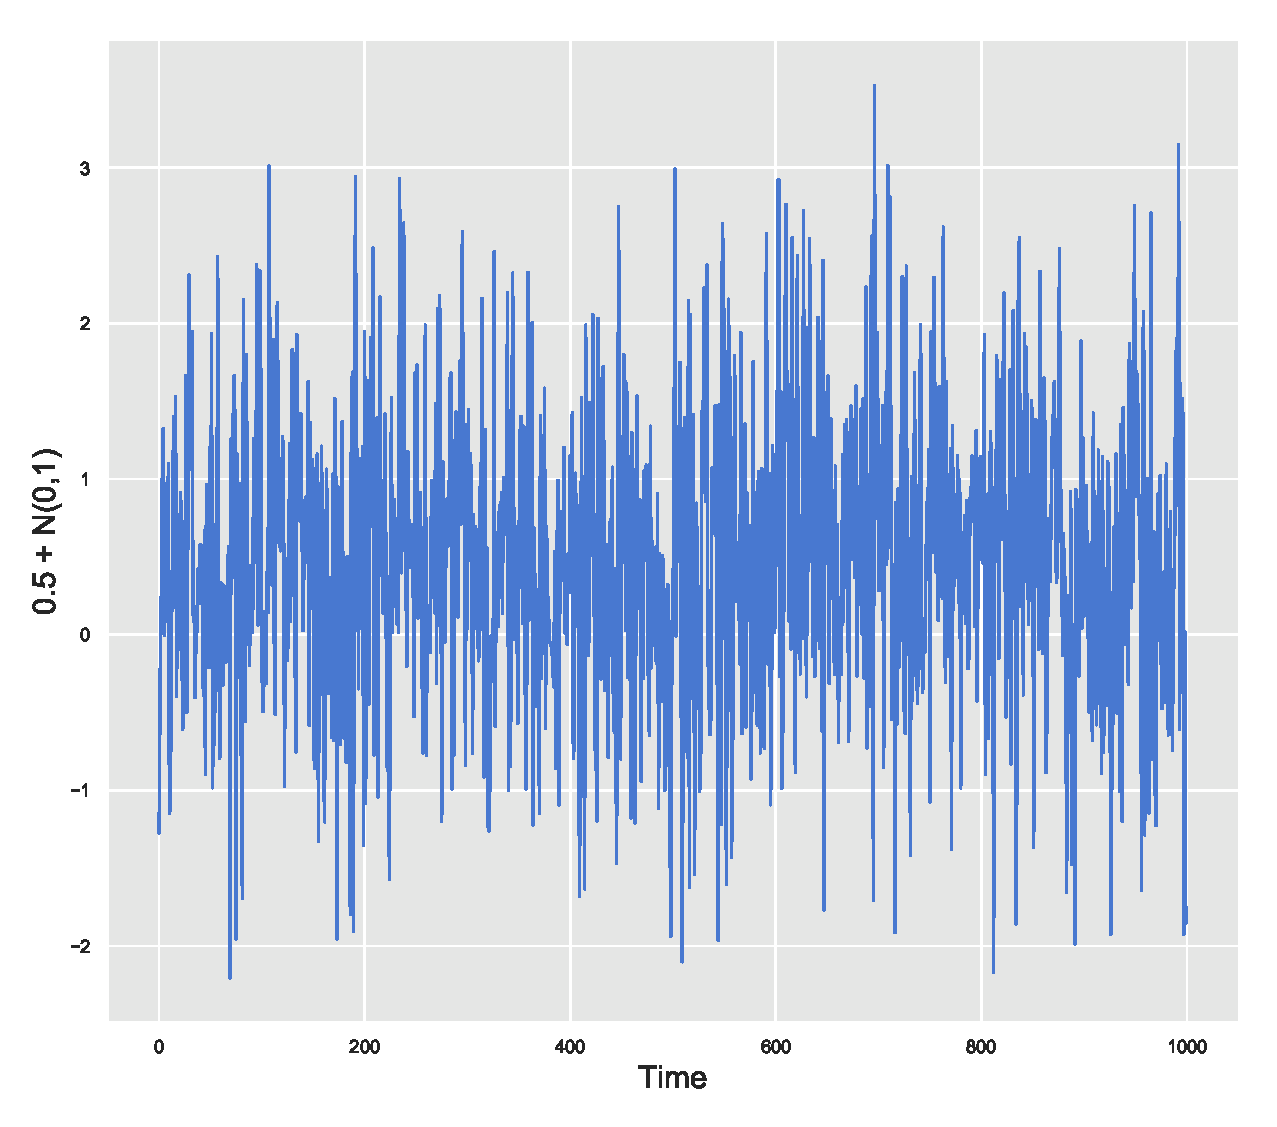
\includegraphics[scale=0.2]{chapters/chapter_uvts/figures/ch1fig1y1ts.eps}
                        }
                        \hfill
                \subfloat[Figure 1b]
                        [ACF]
                        {
                        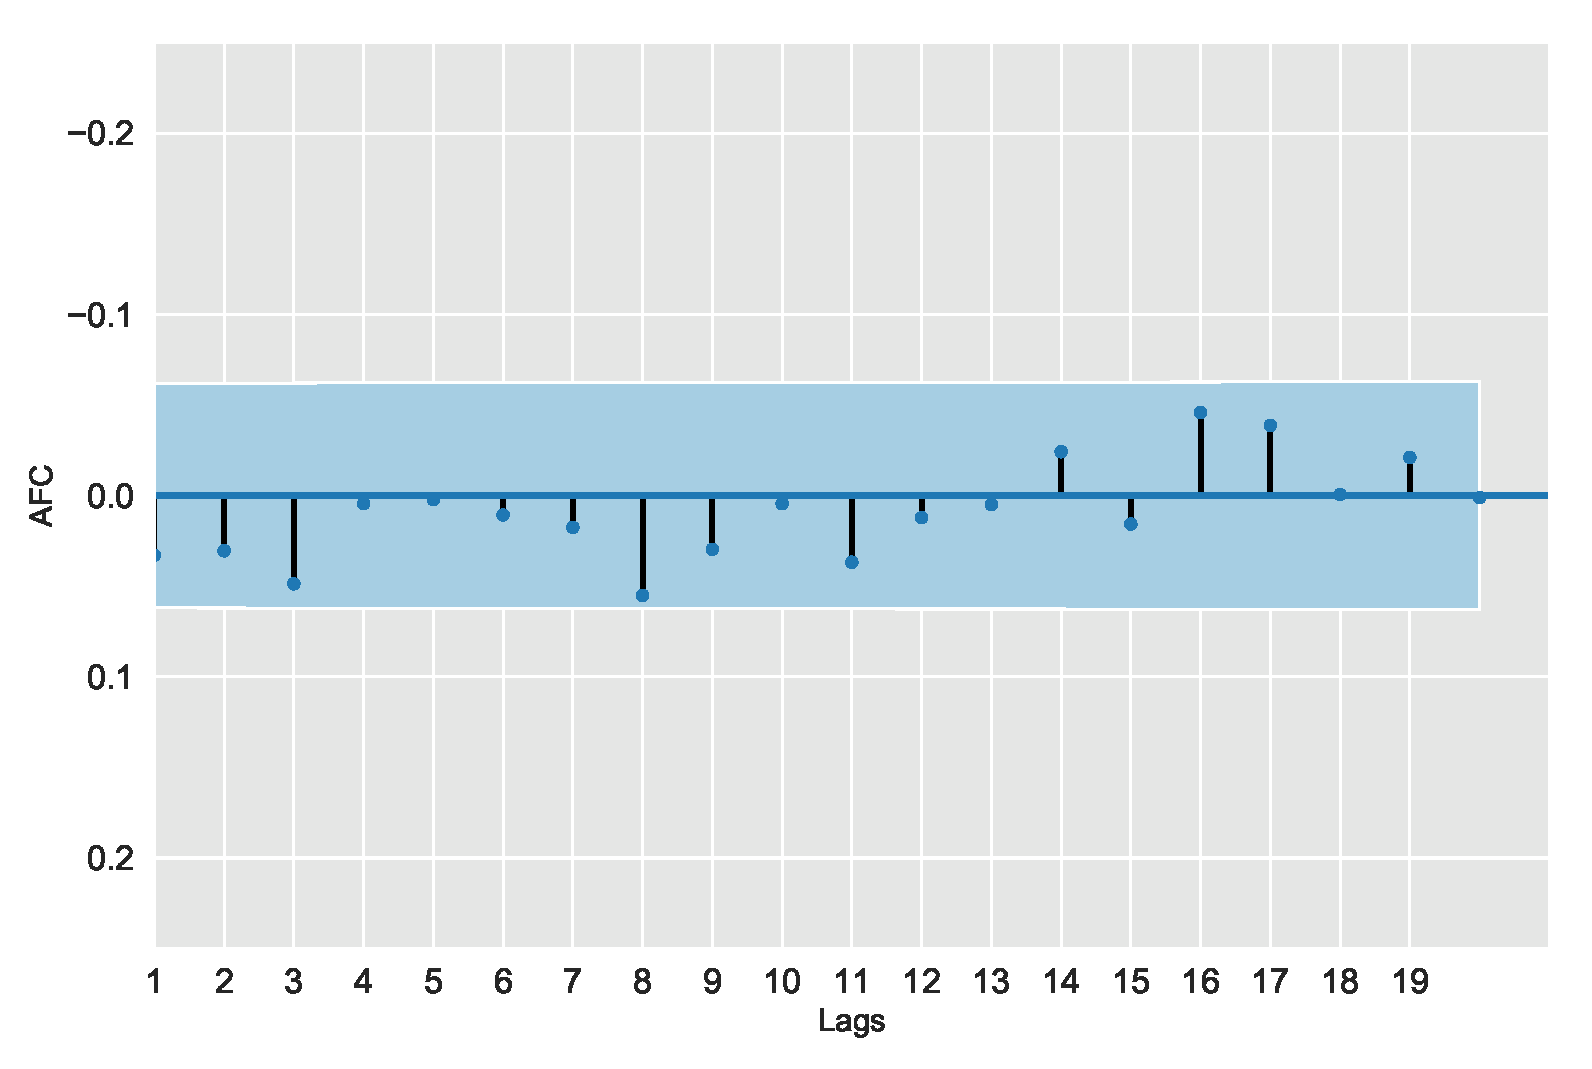
\includegraphics[scale=0.2]{chapters/chapter_uvts/figures/ch1fig1y1acf.eps}
                        } 
                        
                \subfloat[Figure 1c]
                        [$Y_t$ vs. $Y_{t-1}$]
                        {
                        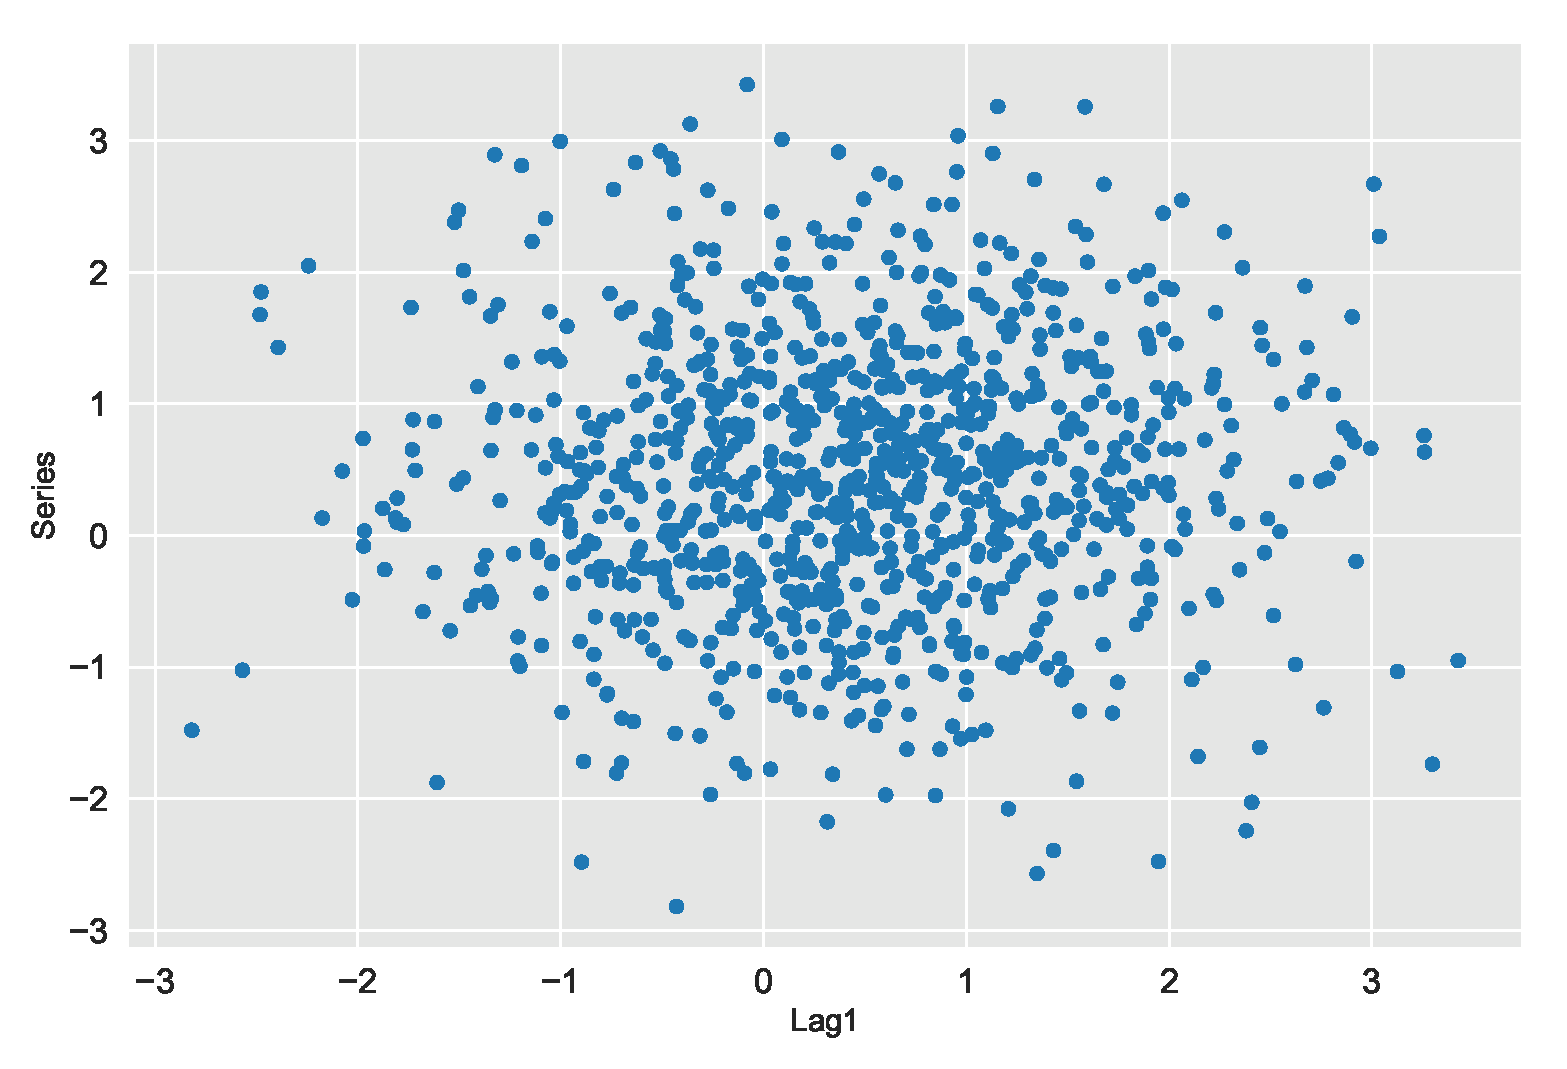
\includegraphics[scale=0.2]{chapters/chapter_uvts/figures/ch1fig1y1lagplot.eps}
                        }
                        \hfill
                \subfloat[Figure 1d]
                        [Time series plot of $1.0 + \epsilon_t + \epsilon_{t-1}$]
                        {
                        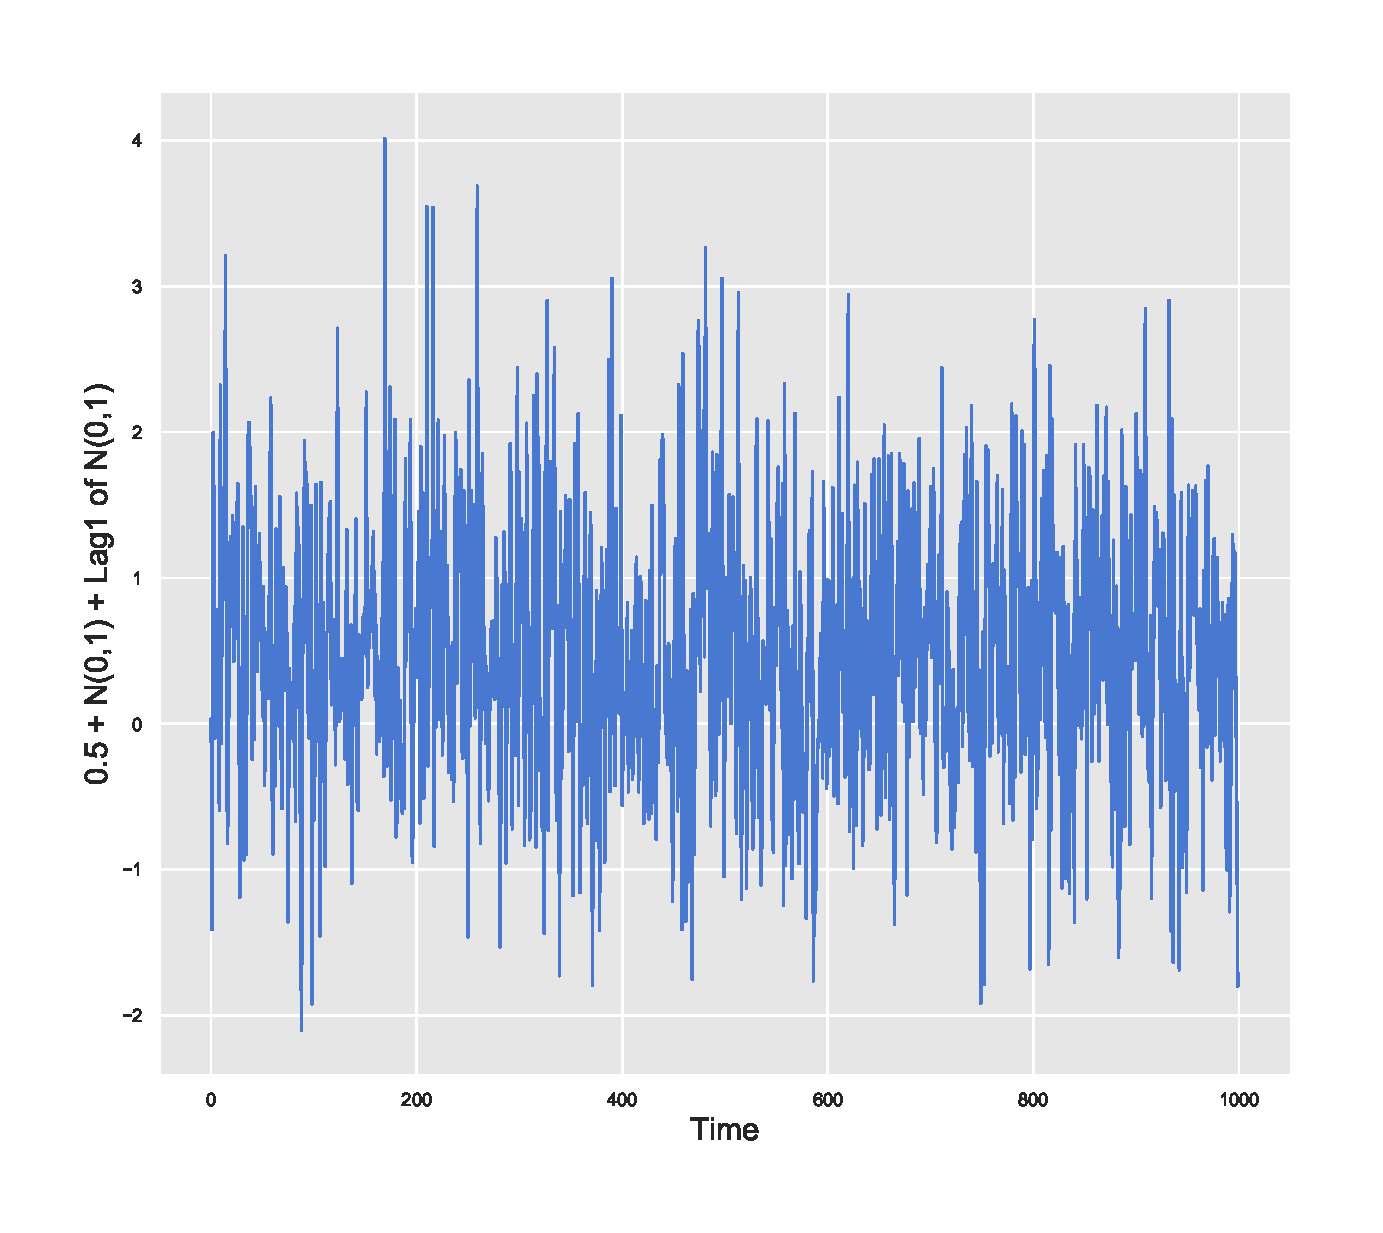
\includegraphics[scale=0.2]{chapters/chapter_uvts/figures/ch1fig1y2ts.eps}
                        }
                        
                \subfloat[Figure 1e]
                        [ACF]
                        {
                        \includegraphics[scale=0.2]{chapters/chapter_uvts/figures/ch1fig1y2acf.eps}
                        }
                        \hfill
                \subfloat[Figure 1f]
                        [$Y_t$ vs. $Y_{t-1}$]
                        {
                        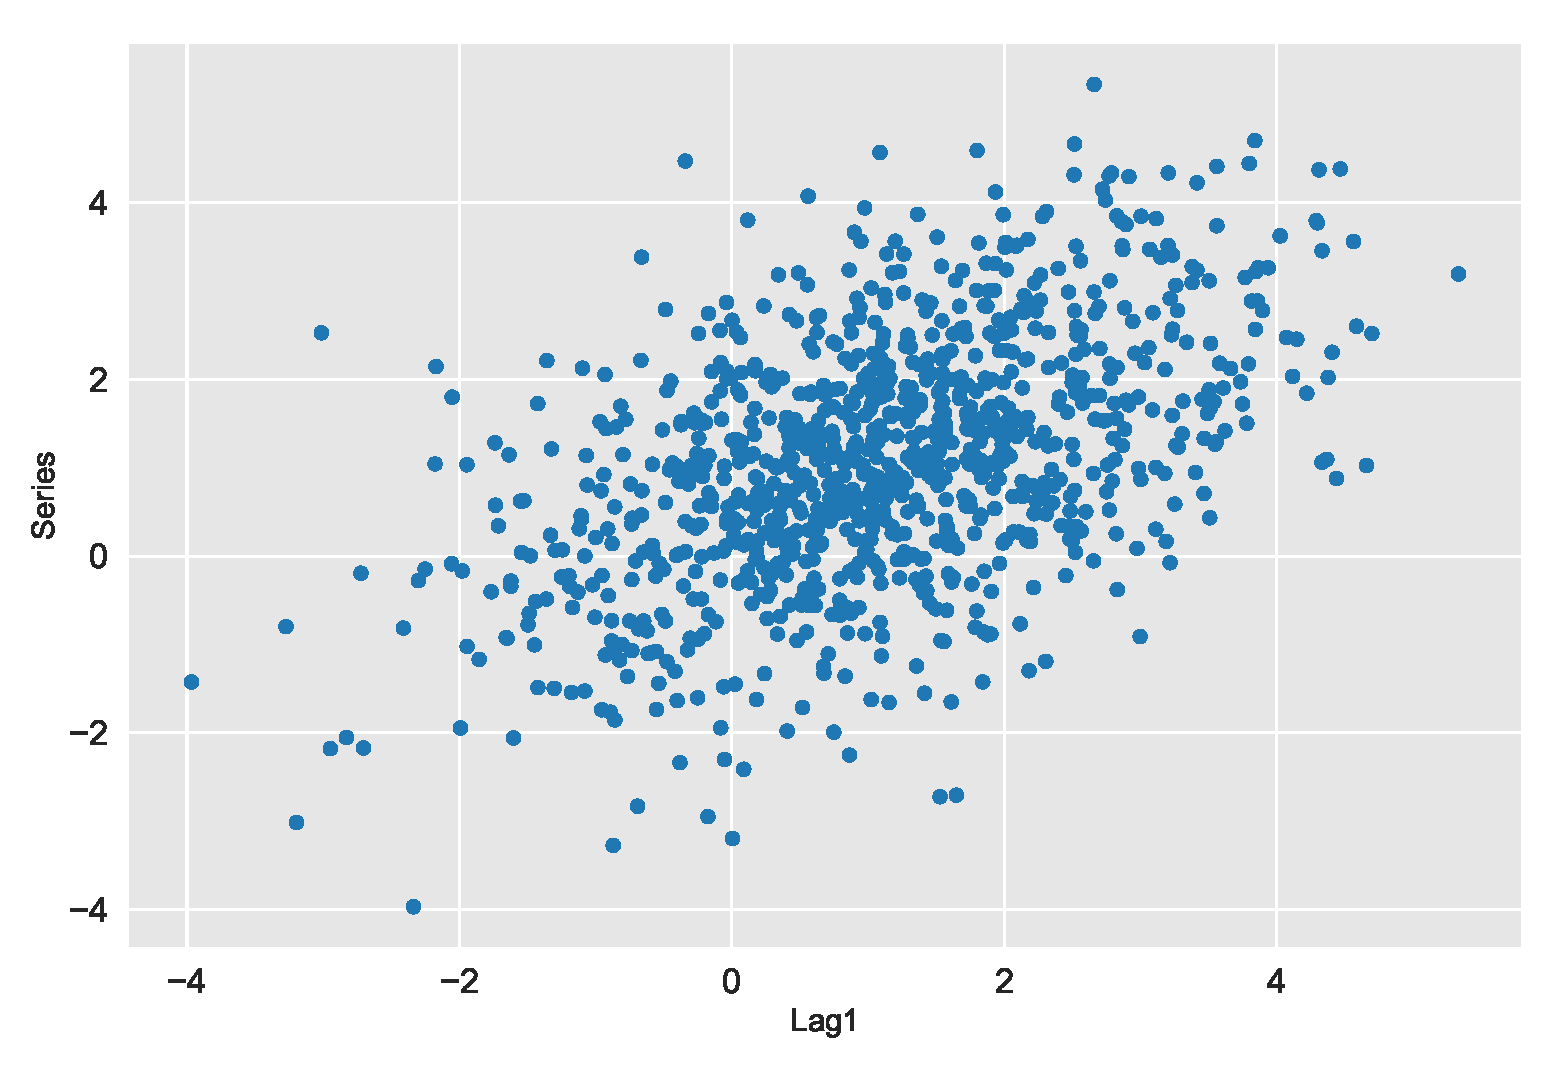
\includegraphics[scale=0.2]{chapters/chapter_uvts/figures/ch1fig1y2lagplot.eps}
                        }
               \caption{Processes \& Diagnostics from $Y_t = 0.5 + \epsilon_t$ and from $Y_t = 1.0 + \epsilon_t + \epsilon_{t-1}$. \label{fig:sideways}}
            \end{sidewaysfigure}


Figure~\ref{fig:sideways}~(a) shows a time series plot of a computer simulated series of 100 values from a Gaussian white noise process $\{ \epsilon_t \}$ with $\sigma^2= 1$, while Figure~\ref{fig:sideways}~(b) shows a plot of the corresponding values of the series $Y_t = 1.0 + \epsilon_{t} + \epsilon_{t-1}$ using these same $\{\epsilon_t\}$.  Note the relatively much smoother behavior over time of the data in (b) than in (a), due to the positive autocorrelation at lag one of the process in (b) which tends to make successive values of the series behave more similarly to each other.  Similar to Example~\ref{ex:movingaverage}, it is easy to show that the process $\{Y_t\}$ defined by the relation $Y_t = \mu + \epsilon_{t} - \epsilon_{t-1}$ is stationary with autocorrelation function $\rho(0)= 1$, $\rho(1)= -1/2$, and $\rho(s)= 0$ for $\lvert s\rvert >1$. A plot of a simulated series from this process is given in Figure~\ref{fig:sideways}~(d) which shows less smooth behavior over time relative to the behavior  in (a) and (b) due to the addition of extra noise to the model. These figures form the basis of model building and the subsequent diagnostic checks on the fitness of models.
\end{ex} 


\noindent \textbf{Examples of Nonstationary Stochastic Processes} \label{in:nonstat1} \twomedskip


Many time series that occur in finance do not exhibit stationary behavior.  For example, stock price series show a trend or shifting mean level over time, reflecting information flow about the stock or investors' behavior. Series also exhibit seasonal behavior, either in the form of nonstationary or deterministic seasonal patterns, both of which need to be distinguished from purely nondeterministic stationary stochastic behavior. Other departures from stationarity include changes in variability of the process over time (nonconstant variance or volatility regimes), abrupt shifts in the mean level, and changes in the autocorrelation structure of the process over time which is a feature of the series which would typically be more difficult to detect.  An important practical matter in the analysis of time series data involves methods of transforming a nonstationary time series into a stationary series, and accounting for and modeling of the nonstationary aspects of the original series. Many of the methods that are found useful in practice involve considering successive changes or differences over time in the original series to remove the nonstationary features of the series, especially changes in the mean level, or using linear regression techniques to help account for the nonstationary mean behavior.  We will illustrate this with a few simple but commonly occurring examples. 


\begin{ex}[Random Walk with a Drift] \label{ex:driftwalk} 
Let $\{ \epsilon_t, \, t=0,1,2, \ldots \}$ be a sequence of independent random variables with mean 0 and variance $\sigma^2$, and define a new process $\{ Y_t \}$ recursively by
	\[
	Y_t = Y_{t-1} + \delta + \epsilon_t, \qquad t=0,1,2, \ldots, \quad Y_0 = 0,
	\]
where $\delta$ is a constant.  By successive substitutions in the above relations for $Y_t$, we find that $\{Y_t\}$ can also be expressed as
	\[
	Y_t = \delta \, t + \sum_{j=1}^t \epsilon_j = \delta \, t + \epsilon_{t} + \epsilon_{t-1} + \cdots + \epsilon_{1}, \qquad t= 1, 2, \ldots .
	\]
Hence we see that $\Ex(Y_t)= \delta t$ and $\var(Y_t)= \var(\sum_{j=1}^t \epsilon_j)= \sum_{j=1}^t \var(\epsilon_j)= t \, \sigma^2$, so that the process $\{ Y_t \}$ is not stationary and exhibits change in both mean and variance.  Moreover, for any $s > 0$, we find that
	\[
	\cov(Y_t,Y_{t+s})= \cov \left( \sum_{j=1}^t \epsilon_j, \sum_{i=1}^{t+s} \epsilon_i \right)= \sum_{j=1}^t \var(\epsilon_j) = t \, \sigma^2 ,
	\]
so that $\corr(Y_t,Y_{t + s}) = t / \sqrt{t(t + s)} = 1/ \sqrt{1 + s/t}$. Note that this correlation is close to one for large $t$ and relatively small $s$, so that nearby values $Y_t$ and $Y_{t+s}$ of the process $\{Y_t\}$ are highly positively correlated.  However, note that the time series of \emph{first differences} of the process $\{ Y_t \}$, defined by $Z_{t}=Y_{t}-Y_{t-1}$, forms a stationary process, because $Z_{t}= Y_{t} - Y_{t-1} = \delta + \epsilon_t$, a white noise series as in Example~\ref{ex:whitenoise}. Such a process $\{ Y_t \}$ whose first differences form a white noise series, is called a random walk process with a drift. Time series plots of simulated data from random walk exhibit behavior with little tendency to vary around a fixed constant mean level. The parameter $\delta$ in the random walk model is referred to as the drift in the random walk process. Note the trend behavior in the process with $\delta > 0$. \xqed
\end{ex}


Of course, a more general class of models is obtained by supposing that a nonstationary process $\{ Y_t \}$ is such that its first differences form a stationary process, but not necessarily white noise.  It has been found from practical experience that this type of model is quite useful in producing adequate representations for actual observed financial series with short term drifts in many cases.



% Some Descriptive Tools and their Properties
\section{Some Descriptive Tools and their Properties} 


Suppose we have a sample realization of $T$ observations $Y_1, Y_2, \ldots, Y_T$ from a stationary process $\{Y_t\}$. We are naturally interested in obtaining estimates of $\mu$, $\gamma(s)$, and $\rho(s)$ from the sample data. First, a natural estimator of $\mu$ is the sample mean $\overline{Y}= (1/T) \sum_{t=1}^T Y_t$. The most common estimator used for $\gamma(s)$ is the sample autocovariance function defined by
	\[
	\hat{\gamma}(s)= \frac{1}{T} \sum_{t=1}^{T-s} \, \left(Y_{t}-\overline{Y}\right) \left(Y_{t+s}-\overline{Y}\right), \quad s=0, 1, \ldots.
	\]
Usually one only computes $\hat{\gamma}(s)$ for lags $s$ much smaller than $T$, say, $0 \leq s \leq T/4$, since $\hat{\gamma}(s)$ for large lags are typically not very informative or of much interest. Note that $\hat{\gamma}(s)$ has the form of an ordinary sample covariance between the pairs of variables $(Y_t, Y_{t+s})$, except for the use of the common sample mean $\overline{Y}$ for both variables and the divisor $T$ in place of $T-s$.  Note also that $\hat{\gamma}(0) = T^{-1}\sum_{t=1}^T (Y_t-\overline{Y})^2$ represents the sample variance of the data.  The estimator of $\rho(s)$ follows directly from $\hat{\gamma}(s)$ and is given by
	\begin{equation} \label{eqn:hatrho}
         \hat{\rho}(s)= \frac{\hat{\gamma}(s)}{\hat{\gamma}(0)}= r(s)= \frac{\sum_{t=1}^{T-s} \left(Y_{t}-\overline{Y}\right) \left(Y_{t+s}-\overline{Y}\right)}{\sum_{t=1}^T(Y_t-\overline{Y})^2} , \quad s= 0, 1, \ldots,
	\end{equation}
which is called the sample ACF.  


We now briefly discuss a few properties of the sampling distributions of the above estimators, with particular emphasis on the sample ACF $r(s)$.  The mean of $\overline{Y}$ is easily seen to be $\Ex(\overline{Y})= (1/T) \sum_{t=1}^T \Ex(Y_t) = \mu$, so that $\overline{Y}$ is an unbiased estimator of $\mu$.  The variance of $\overline{Y}$ is
	\begin{equation} \label{eqn:var}
        \var(\overline{Y})= \frac{\gamma(0)}{T} \left[ 1 + 2 \sum_{u=1}^{T-1} \left(\dfrac{T - u}{T}\right)\, \rho(u) \right].
        \end{equation}
Note that the variance of $\overline{Y}$ needs to account for the autocorrelations. 


The sampling properties of the sample ACF $r(s)$ are quite complicated and exact results are not available except in a few special cases. [See Anderson and Walker (1964)~\cite{anderwalk}.] In the white noise case where the $Y_t$ are independent r.v.'s, we then have $\rho(s)= 0$ for all $s \neq 0$ it can be shown that $\Ex(r(s)) \approx 0$, $\var(r(s)) \approx (T-s)/T^2$, and $\cov(r(s), r(u)) \approx 0$. Hence we can use these results to check for ``non-randomness'' of a series of comparing the sample values $r(s)$ at various lags $s=1, \ldots, k$ with the approximate 95\% limits $\pm \, 2 \sqrt{(T-s)/T^2} \approx 2 / \sqrt{T}$ for the normal distribution to see whether the $r(s)$ generally fall within these limits. We will use this test repeatedly on the residuals as a diagnostic tool for model adequacy. 


In the second case, suppose it is assumed that the theoretical ACF satisfies $\rho(s) = 0$ for all $|s| > q$.  Then for any $s > q$,
	\begin{equation} \label{eqn:varrs}
	\var(r(s)) \approx \dfrac{1}{T} \sum_{\nu=-q}^q \rho(\nu)^2= \dfrac{1}{T} \left[ 1 + 2 \sum_{\nu=1}^q \rho(\nu)^2 \right], \quad s > q 
	\end{equation}        
and
	\[
	\cov(r(s), r(u)) \approx \frac{1}{T} \sum_{\nu = -q}^{q} \rho(\nu)\, \rho(\nu - s + u), \quad s,u > q.
	 \]
As one final special case, suppose the process  has ACF of the simple form (which results from an autoregressive model of order one (AR(1)), with coefficient $\phi$) $\rho(s) = \phi^{|s|}$, $s= 0, \pm 1, \ldots$, with $\lvert \phi \rvert < 1$. Then
	\[
	\var(r(s)) \approx \frac{1}{T} \left[ \frac{(1 + \phi^2) (1 - \phi^{2s})}{1 - \phi^2} - 2s \phi^{2s} \right],
	\]
and in particular $\var(r(1)) \approx \frac{1}{T} (1 - \phi^2)$.


The plot of ACF for a white noise sequence for a large number of lags may have a few isolated lags lie outside the limits, $\pm \frac{2}{\sqrt{T}}$. But characteristic behavior of nonstationary series is that the sample ACF values $r(s)$ are slow to ``dampen out'' as the lag $s$ increases. We will use these facts repeatedly in our analysis. 



% Time Series Models for Aggregated Data:  Modeling the Mean
\section{Time Series Models for Aggregated Data:  Modeling the Mean \label{sec:model_mean}} \label{in:modelmean}

In this section, we present a broad overview of the time series models for data aggregated over discrete time intervals. This data as mentioned in Section~\ref{sec:tradesandquotes} is called price bars and the methodologies discussed in this chapter apply to any aggregated data for fixed time unit of aggregation that is of equal length. As a close substitute for the high frequency data, data aggregated over short time intervals such as two or five minutes can be used. \twomedskip


\noindent\textbf{Linear Models for Stationary Time Series} \twomedskip


A stochastic process $\{ Y_t \}$ will be called a \emph{linear process} if it can be represented as
	\begin{equation} \label{eqn:yt}
          Y_t = \mu + \sum_{j=0}^{\infty}  \psi_j \epsilon_{t-j},
	\end{equation}
where the $\epsilon_t$ are independent with 0 mean and variance $\sigma^2_{\epsilon}$, and $\sum_{j=0}^{-\infty} \lvert \psi_j \rvert < \infty$. This process may also be referred to as an infinite moving average process. With the backward shift operator $B$, defined by the property that $B^j Y_t = Y_{t-j}$, model~\eqref{eqn:yt} may be expressed as
	\[
	Y_t = \mu + \sum_{j=0}^{\infty} \psi_j B^j \epsilon_t = \mu + \psi(B) \epsilon_t,
	\]
where $\psi(B) = \psi_0 + \psi_1 \, B + \psi_2 \, B^2 + \cdots$. Since the input $\{\epsilon_t\}$ is a stationary process, it follows that $\{ Y_t \}$ in \eqref{eqn:yt} forms a stationary process, with mean $\Ex(Y_t)=\mu$ and autocovariance function
	\begin{equation} \label{eqn:covyt}
	\gamma(s)= \cov(Y_t, Y_{t+s})= \sigma^2_{\epsilon} \sum_{j=0}^{\infty} \psi_j \psi_{j+s},
	\end{equation}      
because $\gamma_\epsilon(s) = \sigma^2_\epsilon$ if $s=0$ and $\gamma_\epsilon(s) = 0$ if $s \neq 0$, so that $\gamma_\epsilon(j - k + s) = 0$ when $k \neq j + s$.
	

An important result called Wold's Theorem indicates the generality of the class of linear processes in stationary theory, that every purely non-deterministic stationary process may be expressed in an infinite moving average representation as in \eqref{eqn:yt}, although the $\epsilon_t$ need not be independent but merely uncorrelated.	


The general linear representation model given by \eqref{eqn:yt} although useful for studying the properties of time series models but is not directly useful in practice to represent a stationary process, since it requires the determination of an infinite number of unknown parameters $\psi_1, \psi_2, \ldots$, from a finite set of data. Hence we now consider finite parameter models of the same type which will be useful representations and are sufficiently general to well approximate the model for any process of the form \eqref{eqn:yt}. \twomedskip


\noindent \textbf{Finite Moving Average Processes} \twomedskip


A direct way to obtain finite parameter models from the general form \eqref{eqn:yt} is simply to restrict the $\psi_j$ to be zero beyond some lag $q$. Thus (with a change of notation), a stationary process $\{ Y_t \}$ is said to be a \emph{moving average process} of order $q$, which is denoted as MA($q$), if it satisfies
	\begin{equation} \label{eqn:yt2}
	Y_t = \mu + \epsilon_t - \sum_{j=1}^{q} \theta_j \epsilon_{t-j},
	\end{equation}
where the $\epsilon_t$ are independent with mean 0 and variance $\sigma^2$. Using the backward shift operator notation $B$, the MA($q$) model can be expressed as
	\begin{equation*}
         Y_t= \mu + \theta(B) \, \epsilon_t,	
	\end{equation*}
where $\theta(B) = 1 - \sum_{j=1}^q \theta_j B^j$.  An MA($q$)  process is always stationary, by Wold's Theorem, because $\sum_{j=0}^{\infty} \lvert \psi_j \rvert= 1 + \sum_{j=1}^q \lvert \theta_j \rvert$ is always finite. The mean of the process is $\mu = \Ex(Y_t)$, and the autocovariance function is (from \eqref{eqn:covyt})
	\begin{equation*}
            \gamma(s)= \cov (Y_t, Y_{t+s})= \sigma^2 \sum_{j=0}^{q-s} \theta_j \theta_{j+s}, \quad s = 0, 1, 2, \ldots, q,	
	\end{equation*}
and $\gamma(s)= 0$ for $s > q$, where $\theta_0$ is defined to be $-1$. So in particular, $\gamma(0)=  \var(Y_t) = \sigma^2 (1 + \sum_{j=1}^q \theta_j^2)$. Hence the autocorrelation function of an MA($q$) process \eqref{eqn:yt2} is
       \begin{equation} \label{eqn:rhos}
	\rho(s) = \dfrac{-\theta_s + \sum_{j=1}^{q-s} \theta_j \theta_{j+s}}{1 + \sum_{j=1}^q \theta_j^2}, \quad s = 0,1,\ldots, q
       \end{equation}
and $\rho(s)= 0$ for $s > q$. The prominent feature of the ACF of an MA($q$) process is that it equals zero or ``cuts off'' after a finite number of lags, $q$. Thus in one sense the ``memory'' of an MA($q$) process is $q$ periods long. In practice, useful MA($q$) models are those for which the value of $q$ is typically quite small, such as $q= 1, 2,$ or $3$.  For financial time series, usually $q= 1$ will suffice for modeling, which we will discuss below. 


\begin{ex}[Moving Average Model of Order 1 (MA(1))] \label{ex:movingorder1}
The simplest example of a moving average process is that of order one, MA(1), given by
	\[
	Y_t = \mu + \epsilon_t - \theta \epsilon_{t-1}= \mu + (1 - \theta B)\, \epsilon_t.
	 \]
Its autocovariances are $\gamma(0)= \sigma^2 (1 + \theta^2), \gamma(1)= -\theta\, \sigma^2$, and $\gamma(s)= 0$ for $s > 1$, and hence the ACF is $\rho(1)= -\theta / (1+\theta^2), \rho(s)= 0, s > 1$. It is easy to show that the largest possible value of $\left| \rho(1) \right|= \left| \theta \right| / (1+\theta^2)$ for an  MA(1) process is $\rho(1)= \pm 0.5$ which occurs when $\theta = \pm 1$. This illustrates that in general there are further restrictions on the autocorrelation function $\rho(s)$ of an MA($q$)  process in addition to $\rho(s)= 0, s > q$~.~\xqed
\end{ex}
    

\begin{ex}[Seasonal Moving Average] \label{ex:seasonal} 
For time series which may exhibit seasonal correlation, such as certain financial time series with week-day effect, the following type of special seasonal moving average (SMA) model is useful. Let $S$ denote the number of discrete time periods per seasonal period (for example, $S= 4$ for quarterly data of an annual seasonal nature), and define the process $\{ W_t \}$ by
	\[	
	W_t = \mu + \epsilon_t - \tau_S \, \epsilon_{t-S}.
	\]
Then we find that $\gamma(0)= \sigma^2 (1+\tau_S^2)$, $\gamma(S) = - \tau_S / (1+\tau_S^2)$,  and $\rho(j)= 0$ for all $j \neq 0, \pm S$. Hence this process exhibits nonzero autocorrelation only at the seasonal lag $S$. This model is known as a SMA model of seasonal order 1 (and period $S$), and its generalizations are useful when modeling seasonal differences $W_t = Y_t - Y_{t-S}$ of an original seasonal time series $\{ Y_t \}$.  In the context of financial data, this could be used to model the so-called Monday and Friday effects on price and volatility. \xqed
\end{ex}      


We want to introduce another useful class of models, autoregressive models with the example below.


\begin{ex}[Autoregressive Model of Order 1 (AR(1))] \label{ex:autoregor1}
Consider the process \eqref{eqn:yt} with coefficients given by $\psi_j = \phi^j$, $j= 0,1,\ldots$,  for some $\phi$ with $\lvert \phi \rvert < 1$. Then the process $Y_t = \mu + \sum_{j=0}^{\infty} \phi^j \epsilon_{t-j}$ is stationary, because $\sum_{j=0}^{\infty} \lvert \psi_j \rvert= \sum_{j=0}^{\infty} \lvert \phi \rvert^j = 1/(1 - \lvert \phi \rvert)$ is absolutely convergent for $\lvert \phi \rvert < 1$. From \eqref{eqn:covyt}, the autocovariance function of $\{ Y_t \}$ is
	\[
	\gamma(s)= \sigma^2_{\epsilon} \sum_{j=0}^{\infty} \phi^j \phi^{j+s}= \sigma^2_{\epsilon}\ \phi^s \sum_{j=0}^{\infty} \phi^{2j}= \frac{\sigma^2_{\epsilon} \phi^s}{1 - \phi^2}, \quad s \geq 0.
	\]
In particular, $\gamma(0) = \var(Y_t) = \sigma^2_{\epsilon}/(1-\phi^2)$. Hence the autocorrelation function of $\{ Y_t \}$ is $\rho(s)= \gamma(s) / \gamma(0)= \phi^s$, $ s \geq 0$ which declines exponentially (geometrically) as the lag $s$ increases.


Note that the process $\{Y_t\}$ defined above actually satisfies the relation 
	\[
	Y_t= \phi \, Y_{t-1} + \delta+\epsilon_t,
	\]
$t= \ldots ,-1, 0, 1, \ldots$, with $\delta = \mu(1 - \phi)$. This process is called a first-order autoregressive process, and is a special case of the general class of autoregressive processes which is discussed below. Also note that if the value of $\phi$ in the above is taken as  $\phi = 1$, then the arguments for stationarity of $\{Y_t\}$ no longer hold, because $\sum_{j=0}^{\infty} \lvert \psi_j \rvert = 1 + 1 + \cdots$ does not converge. We see that in this case the process is actually a (nonstationary) random walk satisfying the relation  $Y_t = Y_{t-1} + \epsilon_t$, a common representation of the behavior of the stock prices under the efficient market hypothesis. \xqed
\end{ex}


\noindent\textbf{General Order Autoregressive Processes} \twomedskip


While stock price data exhibit simpler structures such as AR(1) in daily aggregation and returns exhibit MA(1) in smaller time unit aggregation such as five minutes, the volume of trading is shown to have more complex dependencies. The behavior of volume and other trade related data are best captured by higher order (Autoregressive moving average) ARMA models. 


Consider the AR($p$) process $\{ Y_t \}$ defined by
	\begin{equation} \label{eqn:ytsum}
	Y_t = \phi_1 Y_{t-1} + \phi_2 Y_{t-2} + \cdots + \phi_p Y_{t-p} + \delta + \varepsilon_t
	\end{equation}
or $(1 - \phi_1 B - \phi_2 B^2 - \cdots - \phi_p B^p) Y_t = \delta + \varepsilon_t$. When $p= 1$ (Example~\ref{ex:autoregor1}), $Y_t = \phi Y_{t-1} + \delta + \varepsilon_t$, the ACF, $\rho(v)= \phi^{\lvert \nu \rvert}$ takes the simple form, as observed earlier.


\begin{result}
If the roots of $\phi(z) = 1- \phi_1 z - \cdots - \phi_p z^p = 0$ are greater than one in absolute value, then $\{ Y_t \}$ defined by \eqref{eqn:ytsum} is a stationary AR($p$) process and has a one-sided infinite moving average representation as
	\begin{equation} \label{eqn:ytthm}
	Y_t= \mu + \sum_{j=0}^\infty \Psi_j\varepsilon_{t-j},
	\end{equation}
where $\mu = \Ex(Y_t) = \delta / (1 - \phi_1 - \cdots - \phi_p)$, $\Psi(B) = \sum_{j=0}^\infty \Psi_j B^j$. 
\end{result}


The result indicates that if a finite order AR process is modeled as a MA process, it may require a large number of lags. Now we introduce a property based on moments that is useful for estimation of AR models.


The autocovariance $\gamma(s)$ for the AR($p$) process satisfy the \emph{Yule-Walker equations} given by
	\begin{equation*}
	\gamma(s)= \cov(Y_t,Y_{t-s}) = \phi_1 \gamma(s-1) + \phi_2 \gamma(s-2) + \cdots + \phi_p \gamma(s-p), \quad s= 1,2,\ldots,
	\end{equation*}
noting again that $\cov(\varepsilon_t,Y_{t-s})= 0$, for $s > 0$. Dividing by $\gamma(0)$, the ACF $\rho(s)$ also satisfies the relations
	\begin{equation} \label{eqn:rhos2}
	\rho(s) = \phi_1 \rho(s-1) + \phi_2 \rho(s-2) + \cdots + \phi_p \rho(s-p), \quad s= 1,2,\ldots.
	\end{equation}
The Yule-Walker equations \eqref{eqn:rhos2} for $s= 1, 2, \ldots, p$ are particularly useful for determining the autoregressive parameters $\phi_1, \ldots, \phi_p$ in terms of the autocorrelations. Note that these equations can be expressed in matrix form as $P_p \phi = \rho$, where
	\begin{equation} \label{eqn:matrix}
	P_p = 
	\begin{bmatrix}
	1 & \rho(1) & \rho(2) & \cdots & \rho(p-1) \\
	\rho(1) & 1 & \rho(1) & \cdots & \rho(p-2)\\
	\vdots & & \ddots & & \vdots \\
	\rho(p-1) & \cdots & & \rho(1) & 1
	\end{bmatrix}, \quad
	\phi= \begin{bmatrix} \phi_1 \\ \phi_2 \\ \vdots \\ \phi_p \end{bmatrix}, \quad
	\rho= \begin{bmatrix} \rho(1) \\ \rho(2) \\ \vdots \\ \rho(p) \end{bmatrix}.
	\end{equation}
These equations can be used to solve for $\phi_1, \ldots, \phi_p$ in terms of $\rho(1), \ldots, \rho(p)$, with solution $\phi = P_p^{-1} \rho$. Note also, that the variance of the process, $\gamma(0) = \var(Y_t)$, and $\sigma^2= \var(\varepsilon)$, are related by
	\begin{equation} \label{eqn:gamma0cov}
	\gamma(0)= \cov(Y_t, \phi_1 Y_{t-1} + \cdots + \phi_p Y_{t-p} + \delta + \varepsilon_t)= \phi_1 \gamma(1) + \cdots + \phi_p \gamma(p) + \sigma^2,
	\end{equation}
because $\cov(Y_t, \varepsilon_t)= \sigma^2$. Hence $\sigma^2$ can be determined in terms of $\gamma(0)$ and the autocorrelations $\rho(s)$ from \eqref{eqn:gamma0cov}.


Also note that a measure of the strength of association or ``predictability'' of $Y_t$ based on its past values $Y_{t-1}, \ldots, Y_{t-p}$ can be given by the (squared) multiple correlation coefficients of $Y_t$ with $(Y_{t-1}, \ldots, Y_{t-p})$, which is $R^2= (\gamma(0) - \sigma^2)/\gamma(0) = 1 - ( \sigma^2 / \gamma(0) ) = \phi_1 \rho(1) + \cdots + \phi_p \rho(p)$. Since $\gamma(0)$ represents the ``total'' variance of $Y_t$, and $\sigma^2$ may be interpreted as the ``unexplained'' or error variance (i.e., that portion of the variance not explained by the past values), the quantity $R^2$ has the usual interpretation as in linear regression of representing the proportion of the total variance of the variable $Y_t$ that is explained by (auto)regression on the past values $Y_{t-1}, \ldots, Y_{t-p}$. \twomedskip


\noindent\textbf{Partial Autocorrelation Function} \label{in:partac1} \twomedskip


When an AR model is being fit to observed time series data, the sample version of the Yule-Walker equations \eqref{eqn:rhos2}, \eqref{eqn:matrix}, in which the values $\rho(j)$ are replaced by the sample ACF values r(j), can be solved to obtain estimates $\hat{\phi}_j$ of the autoregressive parameters. However, initially it is not known which order $p$ is appropriate to fit to the data. The sample partial autocorrelation function (PACF) will be seen to be useful for determination of the appropriate order of an AR process as how the autocorrelation function (ACF) is useful for the determination of the appropriate order of an MA process. First, we discuss the concept of PACF in general.


Suppose $\{ Y_t \}$ is a stationary process, not necessarily an AR process, with ACF $\rho(j)$. For general $k \geq 1$, consider the first $k$ Yule-Walker equations for the ACF associated with an AR($k$) process.
	\begin{equation} \label{eqn:rhoj}
	\rho(j) = \phi_1 \rho(j-1) + \phi_2 \rho(j-2) + \cdots + \phi_k \rho(j-k), \quad j = 1, 2,\ldots, k
	\end{equation}
and let $\phi_{1k}, \phi_{2k}, \ldots, \phi_{kk}$ denote the solution for $\phi_1, \phi_2, \ldots, \phi_k$ to these equations. Given the ACF $\rho(j)$, \eqref{eqn:rhoj} can be solved for each value $k= 1,2, \ldots$, and the quantity $\phi_{kk}$, regarded as a function of the lag $k$, is called the (theoretical) \emph{partial autocorrelation function} (PACF) of the process $\{ Y_t \}$. The values $\phi_{1k},  \phi_{2k}, \ldots, \phi_{kk}$ which are the solution to \eqref{eqn:rhoj} are the regression coefficients in the regression of $Y_t$ on $Y_{t-1}, \ldots, Y_{t-k}$; that is, values of coefficients $b_1, \ldots, b_k$ which minimize $\Ex[(Y_t - b_0 - \sum_{i=1}^k b_iY_{t-i})^2]$.


If $\{ Y_t \}$ is truly an AR process of order $p$, the $\phi_{kk}$ will generally be nonzero for $k \leq p$, but $\phi_{kk}$ will always be zero for $k > p$. This is so since the ACF $\rho(j)$ actually satisfies the Yule-Walker equations \eqref{eqn:rhoj} for $k= p$, and hence for any $k > p$ the solution to \eqref{eqn:rhoj} must be $\phi_{kk}= \phi_1, \ldots, \phi_{pk}= \phi_p$, $\phi_{p+1,k} = 0, \ldots,\phi_{kk} = 0$, where $\phi_1, \ldots, \phi_p$ are the true AR coefficients. Thus, the PACF $\phi_{kk}$ of an AR($p$) process ``cuts off'' (is zero) after lag $p$, and this property serves to distinguish (identify) an AR($p$) process.


The quantity $\phi_{kk}$ defined above is called the \emph{partial autocorrelation} at lag $k$, since it is actually equal to the partial correlation between the r.v.'s $Y_t$ and $Y_{t-k}$ adjusted for the intermediate variables $Y_{t-1}, Y_{t-2}, \ldots, Y_{t-k+1}$, and $\phi_{kk}$ measures the correlation between $Y_t$ and $Y_{t-k}$ after adjusting for the effects of $Y_{t-1}, Y_{t-2}, \ldots, Y_{t-k+1}$.


Based on a sample $Y_1, \ldots, Y_T$ from a process $\{ Y_t \}$, the sample PACF value at lag $k$, $\hat{\phi}_{kk}$, is obtained as the solution to the sample Yule-Walker equations of order $k$,
	\begin{equation} \label{eqn:rjequation}
	r(j) = \hat{\phi}_{tk} r(j-1) + \cdots + \hat{\phi}_{kk} r(j-k), \quad j = 1, \ldots ,k,
	\end{equation}
for each $k= 1, 2, \ldots$. These are the same form as the equations \eqref{eqn:rhoj} but with sample ACF values $r(j)$ used in place of the theoretical ACF values $\rho(j)$. In matrix notation similar to that used in \eqref{eqn:matrix}, the solution is $\hat{\phi} = R_k^{-1} r$. Now under the assumption that the process $\{ Y_t \}$ is an AR of order $p$, the estimated PACF values $\hat{\phi}_{kk}$ for lags $k > p$ are approximately independently and normally distributed for large $T$, with mean $\Ex(\hat{\phi}_{kk})= 0$ and St.Dev. $\hat{\phi}_{kk} = 1 / \sqrt{T}$ for $k > p$. These facts concerning the sampling properties of the sample PACF $\hat{\phi}_{kk}$ can be used to assess whether the coefficients in estimated AR models may be treated as close to zero after some lag $p$ (e.g. if $\lvert \hat{\phi}_{kk} \rvert < 2 / \sqrt{T}$ for $k > p$), and hence can be useful in the selection of an appropriate order $p$ for fitting an AR model to sample data. \label{in:partac2} \twomedskip


\noindent\textbf{Linear Models for Nonstationary Time Series} \label{in:nonstat2} \twomedskip


Often, in practice, series $\{ Y_t \}$ will be encountered which are nonstationary. One type of nonstationary series that occurs commonly, are series that exhibit some homogeneous behavior over time in the sense that, except for local level and or local trend, one segment of the series may behave much like other parts of the series. In those cases, it may be found that the first difference of the series, $(1 - B)\, Y_t = Y_t - Y_{t-1}$, is a stationary series. For seasonal nonstationary time series that exhibit homogeneous behavior apart from a seasonal mean level or trend, with seasonal period $S$, the seasonal difference of the series, $(1 - B^s)\, Y_t = Y_t - Y_{t-s}$, may be stationary. More generally, a useful class of models for this type of homogeneous nonstationary time series $\{Y_t\}$ is obtained by assuming that the $d$th difference, $W_t = (1 - B)^d\,Y_t$, is a stationary series, and $W_t$ can be represented by an ARMA($p,q$) model. The most common case is $d=1$, for financial time series. \twomedskip


\noindent\textbf{Autoregressive Integrated Moving Average Processes (ARIMA)} \twomedskip


We consider models for $\{ Y_t \}$ such that $W_t = (1 - B)^d\, Y_t$ is a stationary ARMA$(p,q)$ process. The process $\{ Y_t \}$ is then said to be an \emph{autoregressive integrated moving average process} of order $(p,d,q)$, denoted as ARIMA$(p,d,q)$. Since the $d$th differences $W_t$ form an ARMA$(p,q)$ process, they satisfy $\phi(B)\, W_t = \delta + \theta(B)\, \varepsilon_t$. So the ARIMA process $Y_t$ is generated by 
	\begin{equation} \label{eqn:phiBdy}
	\phi(B)(1 - B)^d\, Y_t = \delta + \theta(B)\varepsilon_t,
	\end{equation}
where $\phi(B) = 1 - \phi_1 B - \cdots - \phi_p B^p$ and $\theta(B) = 1 - \theta_1 B - \cdots - \theta_q B^q$.


The use of the term ``integrated'' came as follows. When $d=1$ so that the process $W_t = Y_t - Y_{t-1}= (1-B)Y_t$ is a stationary ARMA$(p,q)$ process. Then the stationary series $W_t$ must be summed or ``integrated'' to obtain the process $\{Y_t\}$; that is,
	\[
	Y_t = (1 - B)^{-1}W_t = (1 + B + B^2 + \cdots)\, W_t = \sum_{j=0}^\infty W_{t-j}. 
	\]
More generally, with $d > 1$, the stationary process $W_t = (1 - B)^d\, Y_t$ must be summed $d$ times to obtain the process $Y_t$. Note that the random walk process \label{in:random1} $Y_t = Y_{t-1} + \delta + \varepsilon_t$ is the simplest example of an integrated process, and is also the most commonly observed in the context of financial time series. Since then the first differences $W_t = Y_t - Y_{t-1} = \delta + \varepsilon_t$ form a (stationary) white noise process, i.e., the process $\{ Y_t \}$ is ARIMA(0,1,0). As noted earlier, this is called a random walk model with a drift.


Differencing is appropriate to apply to processes which contain a stochastic trend component (not a deterministic trend component), and stochastic trend behavior is often more likely to be present in financial time series than deterministic trend behavior. Some observations are in order. First, if a series does not require differencing, over differencing will lead to unnecessarily more complicated models. Second, the differencing can sometimes wipe out all the information leaving series with white noise behavior. Some authors have suggested fractional differencing; that is, $0<d<1$, but there is no theoretic motivation for an appropriate choice of the value of `$d$'. Third, there are identifiability issues in ARMA models; it is possible to model the same data with various ARMA structures, but we will follow the principle of parsimony in modeling. 


Two useful results that we present below to illustrate how the general class of (ARIMA) models \eqref{eqn:phiBdy} can arise in practice.


\begin{result}[Aggregation]
Consider a process $Y_t$, composed of a trend component $U_t$ and a noise component $N_t$, $Y_t = U_t + N_t$. We assume that the (random) trend component follows a random walk model (possibly with a drift), $(1 - B)\, U_t = \delta + a_t$, and we assume that $N_t$ is a stationary AR(1) process $(1 - \phi B)\, N_t = b_t$, where $\{ a_t \}$ and $\{ b_t \}$ are independent white noise processes with zero means and variances $\sigma_a^2$ and $\sigma_b^2$, respectively. Then, applying the first differencing operator, we have $(1 - B)\, Y_t = (1 - B)\, U_t + (1 - B)\, N_t = \delta + a_t + (1 - B)\, N_t$, and hence
	\begin{equation} \label{eqn:bphi}
	\begin{split}
	(1 - \phi B)(1 - B)\,Y_t&= (1 - \phi B)\, \delta + (1 - \phi B)\, a_t + (1 - \phi B)(1 - B)\, N_t \\
	&= (1 - \phi)\, \delta + (1 - \phi B)\, a_t + (1 - B)\, b_t.
	\end{split}
	\end{equation}
It can be shown that $Z_t = (1 - \phi B)\, a_t + (1 - B)\, b_t$ is the sum of two independent MA(1) processes and thus an MA(1) process, so that $Y_t$ is an ARIMA(1,1,1) process. Thus ARIMA $(p, d, q)$ can arise naturally when several stochastic elements with different behaviors are added together. These stochastic elements may come from sources that can be justified by a priori theories. \xqed
\end{result}


This general observation concerning the sum of two ARMA processes gives rise to the following result. 


\begin{result}[Aggregation] \label{thm:agg}
If $X_t$ is an ARMA$(p_1,q_1)$ process and $Y_t$ is an ARMA$(p_2, q_2)$ process, with $X_t$ and $Y_t$ independent process, then $Z_t = X_t + Y_t$ follows an ARMA$(p,q)$ model, where $p \leq p_1 + p_2$ and $q \leq \max(p_1 + q_2, p_2 + q_1)$.
\end{result}


These types of models have potential applications in studying aggregate market behavior of several series. For example in addition to modeling the individual stock behavior in an industry, we can study a model for the entire industry as well. Also where the observed series may be viewed as the sum of the true process of interest plus observational error or noise (as in the classical ``signal-plus-noise'' model), and in the use of structural component models where an observed time series is represented as the sum of unobservable components that correspond to factors such as trend, seasonality, stationary variations, and so on. These are modeled more compactly via Kalman filter which is presented in Chapter~\ref{ch:ch_advanced}. 



% Key Steps for Model Building
\section{Key Steps for Model Building \label{sec:key_step}} \label{in:validation1}

In previous sections, theoretical linear models for stochastic processes and properties implied by these models were discussed. We now consider the problem of identifying appropriate models and fitting them to time series data. The following four steps advocated by George Box highlight the basic stages in the proposed model building and testing procedure:

\begin{enumerate}
\item Model Specification or Identification---specify or identify specific models to be entertained as appropriate, based on preliminary data exploration and examination of certain statistical features, such as features of the sample ACF and PACF for time series data.

\item Parameter Estimation---for the specified model or models, estimate parameters in the tentatively entertained models efficiently.

\item Model Checking---perform diagnostic checks on the adequacy of the estimated model, usually by examination of various features of the residuals from the fitted model.

\item Model Validation---confirm that the model is appropriate for out-of-sample prediction. When multiple models are tried out on a single set of data, it may result in data snooping bias. By keeping the data for building the model and the data for validating the model separate, we avoid the snooping bias. It should be kept in mind that overfit (estimated) models do not perform well in validation.
\end{enumerate}


If the estimated model is assessed as being adequate, it can then be used for forecasting or other purposes of interest. Otherwise, one would return to step one and specify an alternate model or models for further consideration. We now discuss briefly some aspects of the model specification procedures in some detail, and point out the key features. \twomedskip


{\noindent\bfseries\large Model Specification} \twomedskip


Given the time series data $Y_1, \ldots, Y_T$, basic time series  plotting of the series is a fundamental step in the initial model building, along with other data plots that might seem informative. We will then consider the sample ACF and PACF of the original series $Y_t$, and of certain transformed series, such as first and possibly second differences, seasonal differences, logarithms or other instantaneous transformation of the original series, residuals from regression to remove deterministic seasonal component or linear trend, and so on. That is, if the original time series appears to be nonstationary we consider differencing or using residuals from regression methods, of the original series which will yield a \emph{stationary} series. More formal procedures to `test' for certain (unit-root) type nonstationarity can also be considered, and will be discussed later in the context of estimation for AR models.  While dealing with financial time series the following considerations are usually made: for example, $r_t= \text{return} = \ln(P_t) - \ln(P_{t-1})$, where $P_t$ is the price of the stock, the differencing of the log price is naturally considered and for volume $V_t$, because of its size is usually logged $\text{v}_t= \ln(V_t)$ to avoid heteroscedasticity.


The sample ACF and PACF of the stationary series are then compared against features of the theoretical ACFs and PACFs of various types of ARMA models to find an appropriate model for the observed series on the basis of close correspondence in features between sample and theoretical correlation functions. Of course, the sample ACF values that are defined in \eqref{eqn:hatrho} are only \emph{estimates}, and hence are subject to sampling errors. Thus, we must recognize that the sample ACF of an observed series will never correspond in all exact details to an underlying theoretical ACF, and we need to look for correspondence in broad features. To properly interpret the sample ACF $[\hat{\rho}(j)]$, we will use the sampling properties of the estimates $\hat{\rho}(j)$. In particular, under the assumption that $\rho(j) = 0$ for all $j  > q$, we have $\Ex[\hat{\rho}(j)]= 0$ and $\text{St.Dev.}[\hat{\rho}(j)]= \frac{1}{\sqrt{T}}[1 + 2 \sum_{i=1}^q \hat{\rho}(i)^2]^{1/2}$ for $j > q$ and the $\hat{\rho}(j)$ are approximately normally distributed, for moderate and large $T$, a result given in \eqref{eqn:varrs}. Similarly, it is known that if the process $\{Y_t\}$ is an AR of order $p$, then the estimated PACFs for lags $p + 1$ and higher are approximately independently and normally distributed, with $\Ex[\hat{\phi}_{kk}] = 0$ and $\text{St.Dev.}[\hat{\phi}_{kk}] = 1/\sqrt{T}$ for $k > p$. These facts may be used to assess whether the last coefficient in an estimated AR model is essentially zero. We summarize some general patterns of the sample ACF and PACF, which might be useful in the initial model identification step. 


\begin{enumerate}
\item[\textbf{1.}] The sample ACF of a unit-root nonstationary process will not generally dampen out sufficiently fast as the lag increases.

\item[\textbf{2.}] The sample ACF $[\hat{\rho}(j)]$ of a typical stationary process should dampen out sufficiently fast. The general behavior of the (stationary) MA$(q)$, AR$(p)$, and ARMA$(p,q)$ processes is: 

\begin{itemize}
\item MA$(q)$ process has ACF $[\rho(j)]$ that will `cut off' after $q$ lags; that is, $\rho(j) = 0$ for $j > q$. For example, the MA(1) process has $\rho(j)= 0$ for $j > 1$.

\item AR$(p)$ process has ACF$[\rho(j)]$ which can have exponential decay or dampened sinusoidal behavior, or a mixture of both, so this will tend to be the behavior of the sample ACF. For example, the AR(1) process has $\rho(j)=\phi \rho(j-1)$,  or $\rho(j) = \phi^j$, for all $j \geq 1$.

\item ARMA$(p,q)$ process has ACF $[\rho(j)]$ which can have an irregular pattern for the first $q$ lags and then similar behavior to a corresponding AR$(p)$ process for lags greater than $q$. For example, the ARMA(1,1) has $\rho(j) = \phi \rho(j-1)$, or $\rho(j)= \phi^{j-1} \rho(1)$, for $j \geq 2$, which is similar behavior to the AR(1) after lag 1.
\end{itemize}

\item[\textbf{3.}] The sample PACF $\hat{\phi}_{kk}$ is useful to identify the order $p$ of a finite order AR$(p)$ process, because for an AR$(p)$ process the theoretical PACF $\phi_{kk}$ `cuts off' after lag $p$; that is, $\phi_{kk}= 0$ for all $k>p$. For the sample PACF $\hat{\phi}_{kk}$ of an AR$(p)$, we have $\Ex[\hat{\phi}_{kk}]= 0$ and $\text{St.Dev.}[\hat{\phi}_{kk}]=1 / \sqrt{T}$, for $k > p$. 
\end{enumerate} \twomedskip


Although the sample autocorrelation and partial autocorrelation functions are very useful in model identification, in some cases involving mixed ARMA models where they will not provide unambiguous results. There has been considerable interest in developing additional tools for use at the model identification stage. Interested readers can refer to standard texts in time series for more in-depth discussion such as Shumway and Stoffer (2011)~\cite{shumway2011arima}. \twomedskip

                                      
{\noindent\bfseries\large Estimation of Model Parameters} \twomedskip


As there are excellent sources available on this topic, our discussion will be quite brief. \twomedskip


\noindent \textbf{Method of Moments} \twomedskip


Preliminary (initial) estimates of the parameters \eqref{eqn:phiBdy} in the model may be obtained by the \textit{method of moments} procedure, which is based on the sample ACF $\hat{\rho}(j), j= 1, \ldots,  p+q$. The method of moments estimates have the appeal of being relatively easy to compute, but are not statistically efficient (except for a pure AR); they can usefully serve as initial values to obtain more efficient estimates.


Assuming that $W_t= (1 - B)^d\, Y_t$ follows an ARMA$(p,q)$ model, we know that the ACF $\rho(j)$ of $W_t$ satisfies the ``generalized'' Yule-Walker equations in \eqref{eqn:rjequation}. Hence we can obtain initial estimates for the AR parameters $\phi_1, \ldots, \phi_p$ by solving the sample version of these equations for $j= q+1,\ldots, q+p$,
	\begin{equation} \label{eqn:rhohatsum}
	\hat{\rho}(j) - \sum_{i=1}^p \hat{\phi}_i \hat{\rho}(j-i) = 0, \quad j= q+1, \ldots, q+p.
	\end{equation}
Note that these equations could also be useful in identifying the orders $(p,q)$ of an ARMA model. Since the mean $\mu_w = \Ex(W_t)$ of the stationary process $W_t$ in \eqref{eqn:phiBdy} is $\mu_w = \delta/(1 - \phi_1 - \cdots - \phi_p)$, we estimate $\mu_w$ by sample mean $\hat{\mu}_w = \overline{W}$ and hence the constant term $\delta$ by $\hat{\delta}_0 = (1 - \hat{\phi}_1 - \cdots - \hat{\phi}_p)\, \hat{\mu}_w$.


Initial estimates of the MA parameters could then be based on the autocovariances of the `derived' MA(q) process, $W_t^* = \phi(B) W_t = \theta_0 + \theta(B) \varepsilon_t$. The autocovariances of $W_t^*$ are related to those of $W_t$ by
	\begin{equation} \label{eqn:gamseq}
	\gamma(s) = \cov(W_t^*, W_{t+s}^*) = \sum_{i=0}^p \sum_{j=0}^p \phi_i \phi_j \gamma(s+i-j), \quad s = 0,1,\ldots
	\end{equation}
with $\phi_0 = -1$, where $\gamma(j) = \cov(W_t, W_{t+j})$. But since $W_t^* = \theta_0 + \theta(B)\varepsilon_t$ also satisfies the MA($q$) model
	\begin{equation} \label{eqn:gamstareq}
	\gamma_*(s) = \sigma_{\varepsilon}^2 (-\theta_s + \theta_1 \theta_{s+1} + \cdots + \theta_{q-s}\theta_q), \quad s = 1,2,\ldots,q,
	\end{equation}
with $\gamma_*(0) = \sigma_{\varepsilon}^2 (1 + \theta_1^2 + \cdots + \theta_q^2)$. Hence, to obtain initial estimates of $\theta_1, \ldots, \theta_q$ and $\sigma_{\varepsilon}^2$ we first form the estimated autocovariances $\hat{\gamma}_*(s)$ of $W_t^*$ based on \eqref{eqn:gamseq} using the initial $\hat{\phi}_{i}$ and the sample autocovariance $\hat{\gamma}(j)$ of $W_t$. We then substitute the $\hat{\gamma}_*(s)$ for $\gamma_*(s)$ in the equations \eqref{eqn:gamstareq}, and solve for parameters $\theta_1, \ldots, \theta_q$ and $\sigma_{\varepsilon}^2$. The resulting equations are nonlinear in the $\theta_i$ and hence must be solved by an iterative numerical procedure (except for the MA(1) case where an explicit solution is available). We now illustrate this procedure with examples of a few simple models. 


\begin{ex}[AR(1) Model]
 In this case, the only equation needed for the AR parameter $\phi_1$ is the first-order Yule-Walker equation, which gives the estimate $\hat{\phi}_1 = \hat{\rho}(1)$, and then $\gamma(0) = (1- \phi_1^2)\,\gamma(0) \equiv \sigma_{\varepsilon}^2$, so that $\hat{\sigma}_{\varepsilon}^2 = (1 - \hat{\phi}_1^2)\,\hat{\gamma}(0)$. \xqed
 \end{ex}


\begin{ex}[ARMA(1,1) Model]
 The equation for $\phi_1$ comes from $\rho(2) = \phi_1 \rho(1)$, so that the moment estimate is $\hat{\phi}_1 = \hat{\rho}(2) / \hat{\rho}(1)$. Then we can form $\hat{\gamma}(0) = (1+\hat{\phi}_1^2)\,\hat{\gamma}(0) - 2\hat{\phi}_1\,\hat{\gamma}(1)$, $\hat{\gamma}(1) = (1+\hat{\phi}_1^2)\,\hat{\gamma}(1) - \hat{\phi}_1\,\hat{\gamma}(0) - (- \hat{\phi}_1\,\hat{\gamma}(2))$, and solve the equations, $\hat{\gamma}(0) = \sigma_{\varepsilon}^2(1 + \theta_1^2), \hat{\gamma}(1) = -\sigma_{\varepsilon}^2\theta_1$. We have $\hat{\rho}(1) \equiv \hat{\gamma}(1)/\hat{\gamma}(0) = -\hat{\theta}_1/(1 + \hat{\theta}_1^2)$, which leads to the solution to a quadratic equation as $\hat{\theta}_1 = \left(-1 + \sqrt{1-4\hat{\rho}(1)^2} \right) / (2\hat{\rho}(1))$ (provided $\lvert \hat{\rho}(1) \rvert < 0.5$, in which case we get an invertible value with $\lvert \hat{\theta}_1 \rvert < 1$, and then $\hat{\sigma}_{\varepsilon}^2 = \hat{\gamma}(0)/(1+\hat{\theta}_1^2)$. Alternatively, consider directly the sample versions of the first two autocovariance equations for the ARMA(1,1) process, $\hat{\gamma}(0) - \hat{\phi}_1\hat{\gamma}(1) = \sigma_{\varepsilon}^2[1 - \theta_1(\hat{\phi}_1 - \theta_1)]$ and $\hat{\gamma}(1) - \hat{\phi}_1\hat{\gamma}(0) = -\sigma_{\varepsilon}^2\theta_1$

We can eliminate $\sigma_{\varepsilon}^2$ from the above two equations and obtain the initial estimate $\hat{\theta}_1$ by solving a quadratic equation. Then the initial estimate of $\sigma_{\varepsilon}^2$ is $\hat{\sigma}_{\varepsilon}^2 = [\hat{\gamma}(0) - \hat{\phi}_1\hat{\gamma}(1)]/[1 - \hat{\theta}_1(\hat{\phi}_1 - \hat{\theta}_1)]$. This same procedure would specialize to the MA(1) model, with the simplification that the first step of estimation of $\phi_1$ is eliminated and we use simply $\hat{\gamma}(0) = \sigma_{\varepsilon}^2(1 + \theta_1^2)$ and $\hat{\gamma}(1) = -\sigma_{\varepsilon}^2\theta_1$. \xqed
 \end{ex}


\begin{ex}[AR($p$) Model]
 For the AR($p$) model, the method of moments estimates of the $\phi_1$ parameters come directly from solving the system of the first $p$ sample Yule-Walker equations in \eqref{eqn:rhos2} for the series $W_t$. \xqed
\end{ex}


The method of moments can be used for preliminary parameter estimation and also for model specification. Now we will focus on more efficient estimation methods, and the general approach will be the use of Gaussian maximum likelihood (ML) methods, and the closely related method of least squares estimation. This discussion is made brief as there are excellent books such as Shumway and Stoffer (2011)~\cite{shumway2011arima} on these topics. For ease of presentation, we will first examine ML estimation for pure autoregressive models, and extend to the general ARMA model in later sections because certain estimation features are relatively simple for the AR model compared to the general ARMA model. It must be noted that the least-squares estimator does not guarantee that the roots of the characteristic function lie outside the unit circle, but the Yule-Walker estimator does. \twomedskip


\noindent\textbf{Conditional Likelihood Estimation} \twomedskip


We consider parameter estimation for the AR($p$) process with mean $\mu$, or constant term $\delta$.
	\begin{equation} \label{eqn:ytseqagain}
	Y_t = \delta + \sum_{i=1}^p \phi_i Y_{t-i} + \varepsilon_t= \mu + \sum_{i=1}^p \phi_i (Y_{t-i} - \mu) + \varepsilon_t,
	\end{equation}
where $\delta = \mu(1 - \phi_1 - \cdots - \phi_p)$, and we assume the $\varepsilon_t$ are i.i.d. normal N$(0, \sigma^2)$. Given a sample realization of $T$ observations $Y_1, Y_2, \ldots, Y_T$, we consider the conditional likelihood function (i.e., the conditional p.d.f of $Y_{p+1}, \ldots, Y_T$, given the first $p$ observations $Y_1, \ldots, Y_p$. The \emph{conditional maximum likelihood estimates} (CMLE) of $\mu$, $\phi$ and $\sigma^2$ are values of the parameters that maximize the conditional likelihood function, where $\phi$ denotes $(\phi_1,\ldots,\phi_p)$.


First, consider the AR(1) case. Then the conditional (on knowing $y_1$) sum of squares function to be minimized is
	\[
	S_*(\mu,\phi) = \sum_{t=2}^T \big(Y_t - \mu - \phi(Y_{t-1} - \mu) \big)^2 = \sum_{t=2}^T (Y_t - \delta - \phi Y_{t-1})^2.
	\]
Taking $\overline{Y}_{(0)} = \frac{1}{T-1} \sum_{t=2}^T Y_t$ and $\overline{Y}_{(1)} = \frac{1}{T-1} \sum_{t=2}^T Y_{t-1}$, the least squares estimates (LSE) of $\phi$ and $\delta = \mu(1 - \phi)$ are given by
	\[
	\hat{\phi} = \dfrac{\sum_{t=2}^T ( Y_t - \overline{Y}_{(0)} ) (Y_{t-1} - \overline{Y}_{(1)} )}{\sum_{t=2}^T ( Y_{t-1} - \overline{Y}_{(1)}^2 )} ,  \quad \hat{\delta} = \overline{Y}_{(0)} - \hat{\phi}\overline{Y}_{(1)}.
	\]
Now since $\overline{Y}_{(1)} \approx \overline{Y}_{(0)} \approx \overline{Y}$, where $\overline{Y} = (1/T) \sum_{t=1}^T Y_t$ is the overall sample mean, we have approximately that $\hat{\mu} \approx \overline{Y}$, which is an intuitively appealing estimator. Then using $\hat{\mu} \approx \overline{Y}$, we obtain
	\begin{equation} \label{eqn:anotherhatphi}
	\hat{\phi} = \frac{\sum_{t=2}^T(Y_t - \overline{Y}) (Y_{t-1} - \overline{Y} )}{\sum_{t=2}^T (Y_{t-1} - \overline{Y})^2}, \quad \hat{\delta}= (1-\hat{\phi}) \, \overline{Y}.
	\end{equation}
This estimator $\hat{\phi}$ is exactly the estimator one would obtain if the AR equation (adjusted for the overall sample mean $\overline{Y}$) $Y_t - \overline{Y} = \phi(Y_{t-1} - \overline{Y}) + \varepsilon_t, t = 2, \ldots, T$, is treated as an ordinary regression with $Y_{t-1} - \overline{Y}$ as the ``independent'' variable. A further approximation that can be noted from the Yule-Walker equations is $\hat{\phi}= \hat{\rho}(1)$, which is also an appealing estimator since $\rho(1) = \phi$ for the AR(1) process. 


Higher order AR($p$) processes may also be estimated by conditional least squares in a straight forward manner. The estimates are simply obtained by ordinary least squares regression of the ``dependent'' variable $Y_t$ on the ``independent'' variables $Y_{t-1}, \ldots, Y_{t-p}$ and a constant term. Except for the approximation $\hat{\mu} = \overline{Y}$, this approach will produce the conditional least squares estimates. A second approximate method consists of solving the first $p$ sample Yule-Walker equations for $\hat{\phi}_1, \ldots, \hat{\phi}_p$. In matrix notation these sample Yule-Walker equations are $R_p\hat{\phi} = r$ with solution $\hat{\phi} = R_p^{-1} r$, which is the Yule-Walker estimator of $\phi$.


For moderately large sample size $T$, both conditional least squares estimation (``regression'' methods) and Yule-Walker estimation will give approximately the same estimated values of $\phi_1, \ldots, \phi_p$. This is because the sample sums of squares and cross-products that are involved in both estimation methods differ only by ``end-effects'' involving the treatment of the first and/or last few observations in the series. Generally, LS estimators are preferred over YW estimators since they tend to have better ``finite-sample'' properties, especially for AR models that are nearly nonstationary (i.e., have roots of $\phi(B)$ close to the unit circle). For inferences on the AR coefficients, it is observed that $\sqrt{T}\,(\hat{\phi} - \phi)$ converges as $T \to \infty$ to the multivariate normal distribution $N(0,\sigma^2\,\Gamma_p^{-1})$, a multivariate normal with mean 0 and covariance matrix $\sigma^2\,\Gamma_p^{-1}$, where $\Gamma_p \equiv \gamma(0)P_p$, where $P_p$ is defined in \eqref{eqn:matrix}. Thus, for large $T$, we can use the approximation that $\hat{\phi}$ is distributed as $N(\phi,(\sigma^2/T)\,\Gamma_p^{-1})$. For a simple example, in the AR(1) case, the LS or Yule-Walker estimator $\hat{\phi} = r(1) = \hat{\rho}(1)$ has an approximate normal distribution with mean $\phi = \rho(1)$ and variance $\var(\hat{\phi}) = (\sigma^2/T)[\gamma(0)]^{-1} = (1/T)(\sigma^2/\gamma(0)) = (1/T)(1 - \phi^2)$, since $\gamma(0) = \sigma^2/(1 - \phi^2)$ for an AR(1) process, and $\var(\hat{\phi})$ is estimated by $(1 - \hat{\phi}^2)/T$.


The maximum likelihood estimation is based on the augmented conditional likelihood function, augmented with the distribution of the initial values $Y_1, \ldots, Y_p$. The procedure is quite cumbersome, but with large sample, $T$, the distribution of initial values does not make much of a difference in the estimation of the unknown parameters. Maximum likelihood and least squares estimation are much more computationally difficult for a mixed ARMA($p,q$) model than for a pure AR($p$) model because the log-likelihood and the sum of squares are more complicated (non-quadratic) functions of the unknown parameters. Interested readers can refer to standard textbooks in this area, but with financial data which tend to be fairly long, the discussion presented here will suffice. \twomedskip


{\noindent\bfseries\large Model Selection Criteria} \twomedskip


One approach to selecting among competing models is the use of information criteria such as AIC proposed by Akaike (1974)~\cite{akaike74} or the BIC of Schwarz (1978)~\cite{sch78}. They are
	\begin{equation} \label{eqn:aicbic}
	\begin{split}
	\text{AIC}_{p,q}&= \log \hat{\sigma}_\varepsilon^2 + n^* \left( \dfrac{2}{T} \right) \\
	\text{BIC}_{p,q}&=\log\hat{\sigma}_\varepsilon^2 + n^* \left( \dfrac{\log T}{T} \right),
	\end{split}
	\end{equation}
where $\hat{\sigma}_\varepsilon^2$ is the estimated model error variance, and $n^*= p + q + 1$ denote the number of parameters estimated in the model, including the constant term. The first term in the above equations results from the maximized likelihood and can be made smaller with more parameters, while the second term acts as a ``penalty factor'' for the parameters used in the model. In this approach, models which yield a minimum value for the criterion are to be preferred, as these criteria penalize for overfitting. \twomedskip


{\noindent\bfseries\large Model Diagnostics} \label{in:validation2} \twomedskip


As several models can be entertained from specification tools such as ACF and PACF, one quick way to check if all the informative dependencies are captured is to use the model residuals and examine if these residuals reflect the features that are assumed. One key feature is the assumption of independence that can be tested through ACF. Another feature is the constancy in the variance which again can be examined by the plot of squared residuals versus time scale and the time dependence by the ACF of the squared residuals. Thus residuals or functions of the residuals play an important role in model diagnostics. We recommend that descriptive tools should be complemented with visualization tools. \\


{\noindent\bfseries\large Model Validation} \twomedskip


The debate on the evaluation of a model for its consistency with the data at hand or its forecasting power is a long-standing one. The risk of overfitting a model purely by data exploration will be exposed through poor performance in forecasting. There is a chance to develop models that fit the features of the data that may be unique but these features may not be present in the future. We will follow in general the principle of parsimony; that is to develop models with fewer parameters that can adequately represent the data. These models should be robust to extreme values and should be stable over time.


Ideally, model validation requires two random samples from the same population; a training set and a test set. Because of the chronological nature of the time series, usually the training set precedes in time the test set. Thus if $y_t, t= 1,2, \ldots,n_1, n_1+1, \ldots, n_1+n_2$ and if the model is built on `$n_1$' observations and the last `$n_2$' observations are used for model validation, it is usual to compare the prediction mean square error (PMSE),
	\begin{equation} \label{eqn:pmse}
	\text{PMSE} = \sum_{t=1}^{n_2} \frac{(y_{n_1+t} - \,\hat{y}_{n_1+t})^2}{n_2}
	\end{equation}
with the MSE ($\hat{\sigma}_\epsilon^2$) of the fitted model. While other forms of cross-validation methods are applicable to non-dependent data, the method suggested here is usually applied for chronological data.



% Testing for Nonstationary (Unit Root) in ARIMA Models
\section{Testing for Nonstationary (Unit Root) in ARIMA Models: To Difference or Not To \label{sec:diffornot}} 


The decision concerning the need for differencing is based, informally, on features of the time series plot of $Y_t$ and of its sample autocorrelation function (eg. failure of the $\hat{\rho}(k)$ to dampen out quickly). This can be formally evaluated further based on the estimates of model parameters. However, it must be kept in mind that distribution theory for estimates of parameters is quite different between stationary and nonstationary models. Much of the notes below follow from Box, Jenkins, Reinsel, Ljung (2015)~\cite{ljung15}


Consider for the simple AR(1) model $Y_t = \phi Y_{t-1} + \varepsilon_t$, $t = 1,2, \ldots, T$, $Y_0 = 0$, testing that $|\phi| = 1$. The least squares (LS) estimator of $\phi$ can be written as,
	\begin{equation} \label{eqn:futurereffirst}
	\hat{\phi} = \dfrac{\sum_{t=2}^T Y_{t-1}Y_t}{\sum_{t=2}^T Y_{t-1}^2} = \phi + \dfrac{\sum_{t=2}^T Y_{t-1}\varepsilon_t}{\sum_{t=2}^T Y_{t-1}^2}.
	\end{equation}
If the process is stationary, $\lvert \phi \rvert< 1$ as it has been noted earlier, $T^{1/2}(\hat{\phi} - \phi)$ has an approximate normal distribution with zero mean and variance $(1 - \phi^2)$. However, when $\phi = 1$, so $Y_t = \sum_{j=0}^{t-1}\varepsilon_{t-j} + Y_0$, with $\var(Y_t) = \Ex(Y_t^2) = t \sigma^2$, it can be shown that $T(\hat{\phi} - 1) = T^{-1} \sum_{t=2}^T Y_{t-1} \varepsilon_t/T^{-2} \sum_{t=2}^T Y_{t-1}^2$, the estimator $\hat{\phi}$ approaches its true value $\phi = 1$ with increasing sample size $T$ at a faster rate than in the stationary case. Both the numerator and the denominator of the above expression have non-normal limiting distributions. 


We present the commonly used ``Studentized'' statistic, for testing $H_0: \, \lvert \phi \rvert=1$ vs $H_a: \, \lvert \phi \rvert < 1$,
	\begin{equation} \label{eqn:hattaunew}
	\hat{\tau} = \dfrac{\hat{\phi} - 1}{s_{\varepsilon} \left( \sum_{t=2}^T Y_{t-1}^2 \right)^{-1/2}},
	\end{equation}
where $s_\varepsilon^2 = (T - 2)^{-1} (\sum_{t=2}^T Y_t^2 - \hat{\phi} \sum_{t=2}^T Y_{t-1} Y_t)$ is the residual mean square, has been considered. The limiting distribution of the statistic $\hat{\tau}$ has been derived, and tables of the percentiles of this distribution under $\phi = 1$ are given in Fuller (1996)~\cite{fuller1996}. The test rejects $\phi = 1$ when $\hat{\tau}$ is ``too negative.''


For higher order AR($p+1$) model $Y_t = \sum_{j=1}^{p+1}\varphi_j Y_{t-j} + \varepsilon_t$, it is seen that the model can be expressed in an equivalent form as $W_t = (\rho - 1)\, Y_{t-1} + \sum_{j=1}^p \phi_jW_{t-j} + \varepsilon_t$, where $W_t = Y_t - Y_{t-1}$, $\rho - 1 = -\varphi(1) = \sum_{j=1}^{p+1} \varphi_j - 1$, and $\phi_j = -\sum_{i=j+1}^{p+1} \varphi_i$. Hence, the existence of a unit root in $\varphi(B)$ is equivalent to $\rho = \sum_{j=1}^{p+1} \varphi_j = 1$. Thus from the regression estimates of the model, 
	\begin{equation} \label{eqn:wtnew}
	W_t  = (\rho - 1)\, Y_{t-1} + \sum_{j=1}^p \phi_j W_{t-j} + \varepsilon_t ,
	\end{equation}
it has been shown by Fuller (1996)~\cite[Chapter 10]{fuller1996} that $(\hat{\rho} - 1)/[s_\varepsilon(\sum_{t=p+2}^T Y_{t-1}^2)^{-1/2}]$ has the same limiting distribution as the statistic $\hat{\tau}$ in \eqref{eqn:hattaunew} for the AR(1) case.


The above methods extend to the case where a constant term is included in the least squares regression estimation, with the statistic analogous to $\hat{\tau}$ denoted as $\hat{\tau}_\mu$. Thus, for example, in the AR(1) model $Y_t = \phi Y_{t-1} + \theta_0 + \varepsilon_t$, one obtains the least squares estimate,
	\begin{equation} \label{eqn:hatphinewest}
	\widehat{\phi}_{\mu} = \dfrac{\sum_{t=2}^T(Y_{t-1} - \overline{Y}_{(1)})(Y_t - \overline{Y}_{(0)})}{\sum_{t=2}^T(Y_{t-1} - \overline{Y}_{(1)})^2},
	\end{equation}
where $\overline{Y}_{(i)} = (T - 1)^{-1}\sum_{t=2}^TY_{t-i}$, $i = 0,1$. The corresponding test statistic for $\phi = 1$ in the AR(1) case is
	\begin{equation} \label{eqn:anotherhattau}
	\hat{\tau}_\mu = \dfrac{\widehat{\phi}_\mu - 1}{s_{\varepsilon} \left( \sum_{t=2}^T(Y_{t-1} - \overline{Y}_{(1)})^2 \right)^{-1/2}}
	\end{equation}
and percentiles of the distribution of $\hat{\tau}_\mu$ and when $\phi = 1$ are given in Table~\ref{tab:percentiles}.

	\begin{table}[!ht]
	\centering
	\caption{Approximate percentiles \label{tab:percentiles}}
	\begin{tabular}{crrrrrrrr}
	& \multicolumn{7}{c}{Probability of a Smaller Value} \\
	& 0.01 & 0.025 & 0.05 & 0.10 & 0.90 & 0.95 & 0.975 & 0.99 \\ \hline
	$\hat{\tau}$ & $-2.58$ & $-2.23$ & $-1.95$ & $-1.62$  &0.89 & 1.28 & 1.62 & 2.00 \\
	$\hat{\tau}_\mu$ & $-3.43$ & $-3.12$ & $-2.86$ & $-2.57$ & $-0.44$ & $-0.07$ & 0.23 & 0.60
	\end{tabular}
	\end{table}


\begin{ex}[To difference or not] 
To illustrate here, we consider briefly the quarterly series of U.S. Commercial Paper interest rates for 1953--1970 in Figure~\ref{fig:exchratefirst}. The series is identified as ARIMA(1,1,0), and unconditional least squares estimation gave 
	\[
	W_t = (1 - B)\, Y_t = 0.4326\, W_{t-1}.
	\]
When conditional LS estimation of an AR(2) model for $Y_t$, as represented in \eqref{eqn:wtnew}, was performed, the results were $W_t = -0.0647Y_{t-1} + 0.478 W_{t-1} + 0.277$, and the estimate $\hat{\rho} - 1 = -0.0147$ had estimated standard error of $0.0317$. Clearly, the test statistic $\hat{\tau} = -2.04$ is not significant, and there is no cause to doubt the need for first differencing of the series $Y_t$ (i.e., that there is a unit root for $Y_t$).
	\begin{figure}[!ht]
	\centering
	\includegraphics[width=\textwidth]{chapters/chapter_uvts/figures/uscompaper.eps}
	\caption{U.S. Commercial Paper Interest Rate.\label{fig:exchratefirst}}
	\end{figure}
The use of the unit root test statistics will become apparent when we discuss pairs trading based on co-integration (see Chapter~\ref{ch:stat_ts}). A precondition for forming co-integrated pairs is that each series must be non-stationary on its own. \xqed
\end{ex}



% Forecasting for ARIMA Processes
\section{Forecasting for ARIMA Processes} \label{in:forecast1}

Given a realization of ARIMA($p,d,q$) process through time t, $\{ Y_s, s \leq t \}$, we consider the problem of forecasting of future values $Y_{t+l}, l = 1,2, \ldots$. For this purpose, it is assumed that the model for $\{ Y_t \}$ is known exactly including the values of the model parameters. Although, in practice, the model parameters are estimated from available sample data, errors due to estimation of parameters will not have too much effect on forecast properties for sufficiently large sample sizes. Also, the practical problem of future values based on the finite past sample data $Y_1, \ldots, Y_T$ will be considered briefly, but results based on the infinite past data assumption usually provide an adequate approximation to the finite past data prediction problem. \twomedskip


\noindent \textbf{Minimum Mean Squared Error Prediction} \twomedskip


Before presenting details of forecasting for ARIMA processes, we review some basic principles concerning prediction in the regression setting. Let $Y$ be a r.v. and let $X = (X_1, \ldots, X_p)'$ be an $p$-dimensional random vector related to $Y$, and consider the problem of predicting (estimating) the unknown value of $Y$ by some function of $X$, say $\hat{Y} = g(x)$. The mean squared error (MSE) of a predictor $\hat{Y}$ is $\Ex[(Y - \hat{Y})^2]$. We refer to the minimum mean squared error (minimum MSE) predictor of $Y$ as that function $\hat{Y} = g^*(X)$ such that, among all possible functions of $X$, $\hat{Y}$ minimizes the MSE $\Ex[(Y - \hat{Y})^2]$. Then it is well-known that the \emph{minimum mean squared error} predictor is given by $\hat{Y} = \Ex(Y\;|\;X)$, the conditional expectation of $Y$ given $X$, with prediction error $e = Y - \hat{Y} = Y - \Ex(Y\;|\;X)$. One can also restrict prediction to consider only linear functions of $X$, and hence consider the minimum MSE \emph{linear} predictor as the linear function $\hat{Y}^* = a + b' X$ which minimizes the prediction MSE among all linear functions of $X$. It is well-known that the minimum MSE linear predictor is
	\begin{equation} \label{eqn:2yhatstar}
	\hat{Y}^* = \mu_y + \Sigma_{yx}\,\Sigma_{xx}^{-1}(X - \mu_x)
	\end{equation}
with the prediction error $e^* = Y - \hat{Y}^*$ having mean zero and prediction MSE (variance)
	\begin{equation} \label{eqn:2varestar}
	\var(e^*) = \var(Y - \hat{Y}^*) = \sigma_y^2 - \Sigma_{yx}\,\Sigma_{xx}^{-1}\,\Sigma_{xy},
	\end{equation}
where $\mu_y = \Ex(Y), \mu_x = \Ex(X)$, $\sigma_y^2 = \var(Y)$, $\Sigma_{yx} = \cov(Y,X)$, and $\Sigma_{xx} = \cov(X)$. Note $\Sigma_{yx}$ is a $1 \times p$ row vector and $\Sigma_{xx}$ is a $p \times p$ variance-covariance matrix. Moreover, if the prediction error $e^* = Y - \hat{Y}^*$ of the best linear predictor is such that $\Ex(e^*\;|\;X) = 0$ (e.g., if $e^*$ is independent of $X$), then $\hat{Y}^*$ is also the minimum MSE predictor, i.e. $\hat{Y}^* = \hat{Y} = \Ex(Y\;|\;X)$ is a linear function of $X$ and the prediction error $e = e^* = Y - \hat{Y}$ has variance $\var(e^*)$ as given above in \eqref{eqn:2varestar}. \twomedskip


\noindent\textbf{Forecasting for ARIMA Processes and Properties of Forecast Errors} \twomedskip


For forecasting in the time series setting, we assume that the process $\{ Y_t \}$ follows an ARIMA$(p,d,q)$ model, $\phi(B)(1 - B)^d\,  Y_t = \theta(B) \varepsilon_t$, and we assume the white noise series $\varepsilon_t$ are mutually independent random variables. We are interested in forecasting the future value $Y_{t+l}$ based on observations $Y_t,Y_{t-1},\cdots$. From the result in previous section, the minimum MSE forecast of $Y_{t+l}$ based on $Y_t, Y_{t-1}, \ldots$, which we will denote as $\hat{Y}_t(l)$, is such that $\hat{Y}_t(l) = \Ex(Y_{t+l} \;|\; Y_t,Y_{t-1},\ldots)$. The prediction $\hat{Y}_t(l)$ is called the lead $l$ or $l$-step ahead forecast of $Y_{t+l}$, $l$ is the lead time, and $t$ is the forecast origin.


To obtain a representation for $\hat{Y}_t(l)$, recall the ARIMA process has the ``infinite'' MA form $Y_t = \psi(B) \varepsilon_t = \sum_{i=0}^{\infty}\psi_i \varepsilon_{t-i},$ and hence a future value $Y_{t+l}$ at time $t+l$, relative to the current time or ``forecast origin'' t, can be expressed as
	\begin{equation} \label{eqn:2ytl}
	Y_{t+l} = \sum_{i=0}^\infty \psi_i \varepsilon_{t+l-i} = \sum_{i=0}^{l-1} \psi_i \varepsilon_{t+l-i} + \sum_{i=l}^\infty \psi_i \varepsilon_{t+l-i}.
	\end{equation}
The information contained in the past history of the $Y_t's, \{ Y_s, s \leq t \}$, is the same as that contained in the past random shocks $\varepsilon_t$'s (because the $Y_t$'s are generated by the $\varepsilon_t$'s). Also, $\varepsilon_{t+h}$, for $h > 0$ is independent of present and past values $Y_{t}, Y_{t-1}, \ldots$, so that $\Ex(\varepsilon_{t+h} \;|\; Y_t,Y_{t-1},\ldots) = 0, h>0$. Thus
	\begin{equation} \label{eqn:2yhatt}
	\hat{Y}_t(l) = \Ex(Y_{t+l} \;|\; Y_t,Y_{t-1},\ldots) = \Ex(Y_{t+l} \;|\; \varepsilon_t, \varepsilon_{t-1}, \ldots) = \sum_{i=l}^\infty \psi_i \varepsilon_{t+l-i},
	\end{equation}
using the additional property that $\Ex(\varepsilon_{t+l-i} \;|\; \varepsilon_t,  \varepsilon_{t-1}, \ldots) = \varepsilon_{t+l-i}$ if $i \geq l$. The $l$-step ahead prediction error is given by $e_t(l) = Y_{t+l} - \hat{Y}_t(l) = \sum_{i=0}^{l-1} \psi_i \varepsilon_{t+l-i}$. So we have $\Ex[e_t(l)]=0$ and the mean squared error or variance of the $l$-step prediction error is
	\begin{equation} \label{eqn:2sigmasq}
	\sigma^2(l) = \var(e_t(l)) = \Ex[e_t^2(l)] = \var \left(\sum_{i=0}^{l-1} \psi_i \varepsilon_{t+l-i} \right) = \sigma^2 \sum_{i=0}^{l-1} \psi_i^2,
	\end{equation}
with St.Dev. $(e_t(l)) = \sigma(l) = \sigma(1 + \psi_1^2 + \cdots + \psi_{l-1}^2)^{1/2}$. Note, in particular, that for $l = 1$ step we have $e_t(1) = Y_{t+1} - \hat{Y}(1) = \varepsilon_{t+1}$ with error variance $\sigma^2 = \var(\varepsilon_{t+1})$, so that the white noise series $\varepsilon_t$ can also be interpreted as the one-step ahead forecast errors for the process. Under the normality assumption that the $\varepsilon_t$ are normally distributed as i.i.d. $N(0, \sigma^2)$, the $l$-step ahead forecast errors $e_t(l) = Y_{t+l} - \hat{Y}_t(l) = \sum_{i=0}^{l-1} \psi_i \varepsilon_{t+l-i}$ will also be normally distributed with mean 0 and variance $\sigma^2(l) = \sigma^2 \sum_{i=0}^{l-1} \psi_i^2$. Hence, the conditional distribution of $Y_{t+l}$, given $Y_t,Y_{t-1}, \ldots$, is normal with mean $\hat{Y}_t(l)$ and variance $\sigma^2(l)$.


For forecasting purposes, the variance $\sigma^2(l)$ of the $l$-step forecast error provides a measure of the degree of accuracy of the point forecast $\hat{Y}_t(l)$. Along with the point forecast $\hat{Y}_t(l)$, we need to provide prediction intervals for the future observations $Y_{t+l}$ so that the degree of uncertainty of the point forecasts is properly reflected. From the preceding paragraph, it follows that the standardized variable $Z_t(l) = e_t(l) / \sigma(l)= ( Y_{t+l} - \hat{Y}_t(l) ) / \sigma(l)$ is distributed as standard normal $N(0,1)$, which is also the conditional distribution of this variable, given $Y_t, Y_{t-1}, \ldots$. Then, for example, from $0.90 = R[-1.65 < Z_t(l) < 1.65] = P[\hat{Y}_t(l) - 1.65\,\sigma(l) < Y_{t+l} < \hat{Y}_t(l) + 1.65\,\sigma(l)]$, it follows that a $90\%$ prediction interval (interval forecast) for $Y_{t+l}$ is given by $\hat{Y}_t(l) \pm 1.65 \sigma(l)$, where $\sigma(l) = \sigma( \sum_{i=0}^{l-1} \Psi_i^2 )^{1/2}$. Prediction intervals for other desired levels of confidence, $100(1 - \alpha)\%$, can be constructed similarly. Of course, in practice, estimates of $\sigma^2$ and of the weights $\psi_i$ based on the estimates $\hat{\phi}_i$ and $\hat{\theta}_i$ of parameters in the ARIMA model obtained from the sample data will actually be used in estimating the standard deviation $\sigma(l)$ of the forecast errors and in forming the prediction intervals. 


\begin{ex}[IMA(1,1) Model]
 Let $Y_t - Y_{t-1} = \delta + \varepsilon_t - \theta\varepsilon_{t-1}$. Then, from \eqref{eqn:2ytl}--\eqref{eqn:2yhatt}, the forecasts are $\hat{Y}_t(1) = Y_t + \delta -\theta\varepsilon_t$, $\hat{Y}_t(2) = Y_t(1) + \delta = Y_t -\theta\varepsilon_t + 2\delta$, and in general,
	\[
	\hat{Y}_t(l) = \hat{Y}_t(l-1) + \delta = Y_t - \theta\varepsilon_t + \delta(l) = \hat{Y}_t(1) + \delta(l-1),\quad l= 1, 2, \ldots
	\]
So the ``eventual'' forecast function $\hat{Y}_t(l)$ is a straight line with a deterministic (fixed) slope $\delta$, and an ``adaptive'' intercept $\hat{Y}_t(1) - \delta = Y_t - \theta \varepsilon_t$ which is random and is adaptive to the process values which occur through time t. The variance of the $l$-step ahead forecast error $e_t(l)$ is $\sigma^2(l) = \sigma^2 (1 + (l-1)(1-\theta)^2), l \geq1$. Hence, we see that the values $\sigma^2(l)$ increase without bound as the lead time $l$ increases, which is a general feature for (nonstationary) ARIMA processes with $d > 0$. Also notice from the infinite AR form of the model (with $\delta = 0$) with AR coefficients $\pi_i = (1-\theta\,)\theta^{i-1}$, $i \geq 1$, $Y_{t+1} = (1-\theta)\sum_{i=1}^\infty \theta^{i-1}Y_{t+1-i} + \varepsilon_{t+1}$, we have the representation $\hat{Y}_t(1) = (1-\theta)\sum_{i=1}^\infty \theta^{i-1} Y_{t+1-i}$. This provides the exponential smoothing, or exponentially weighted moving average (EWMA), form of the one-step forecast $\hat{Y}_t(1)$ in the IMA(1,1). This model with a short term drift `$\delta$' is of immense interest in modeling the stock prices. \xqed
\end{ex}



% Stylized Models for Asset Returns
\section{Stylized Models for Asset Returns} \label{in:assetret1} \label{in:style1}

It is generally known that the equity market is extremely efficient in quickly absorbing information about stocks: When new information arrives, it gets incorporated in the price without delay. Thus the efficient market hypothesis, is widely accepted by financial economists. It would imply that neither technical analysts that study the past prices in an attempt to predict future prices nor fundamental analysts of financial information related to company earnings and asset values would carry any advantage over the returns obtained from a randomly selected portfolio of individual stocks.


The efficient market hypothesis is usually associated with the idea of the ``random walk'',\label{in:random2} which implies that all future price changes represent random departures from past prices. As stated in Malkiel (2012)~\cite{malkiel}: ``The logic of the random walk is that if the flow of information is unimpeded and information is immediately reflected in stock prices, then tomorrow's price change will reflect only tomorrow's news and will be independent of the price changes today. But news by definition is unpredictable, and, thus resulting price changes must be unpredictable and random.''


The random walk (RW) model (Example~\ref{ex:driftwalk}) without the drift term can be stated as:
	\begin{equation} \label{eqn:2pteq}
	p_t = p_{t-1} + \varepsilon_t,
	\end{equation}
where $\varepsilon_t \sim N(0,\sigma^2)$ i.i.d and $p_t = \ln{(P_t)}$. Note as observed earlier, this model is a particular case of AR(1) model if the constant term is assumed to be zero and the slope, $\phi$, is assumed to be one. Thus, the RW model is a non-stationary model and considering $\varepsilon_t = p_t - p_{t-1}=r_t$ is the differencing of the series, $p_t$, makes the series $\varepsilon_t$ stationary. Note $r_t \approx \frac{P_t - P_{t-1}}{P_{t-1}}$,  the returns are purely random and are unpredictable. For any chronological data the decision concerning the need for differencing is based, informally, on the features of time series plot of $p_t$, its sample autocorrelation function; that is, its failure to dampen out sufficiently quickly. \twomedskip


\noindent\textbf{Testing for a RW model:} \label{in:nonstat3} Consider the AR(1) model $p_t = \phi p_{t-1} + \varepsilon_t$, $t = 1,\ldots,T$ and $p_0$ is fixed; we want to test $\phi = 1$. The details of this test are given in Section~\ref{sec:diffornot}, along with the table of the percentiles of the distribution of the test statistics. While the results for testing for non-stationarity for higher order autoregressive models were discussed earlier, the price series once differenced does not generally exhibit autocorrelation structure that requires modeling beyond AR(1).


It will become obvious in subsequent discussions, that in order to exploit any pattern in the returns, one has to look beyond linear time dependencies. We observe a series of established stylized facts regarding stock prices (returns). \twomedskip


\noindent\textbf{Stylized fact 1: Absence of Autocorrelation in returns:} Linear autocorrelations are often insignificant for a lower frequency data. 


To illustrate the main ideas, we consider the exchange rate between USD and GBP; these are daily closing rates from January 4, 1999 to September 16, 2013. The time series plot of the data in (Figure~\ref{fig:exchrate}) clearly indicates that the price is non-stationary and it is confirmed by the never dying autocorrelation function in (Figure~\ref{fig:exchrate}). The LS estimates $\hat{\phi}= 0.9996$, $s_e= 0.00958$ and $\sum_{t=2}^T p_{t-1}^2 = 10431$, provides a value of $\hat{\tau} = -0.001$ from \eqref{eqn:hattaunew} which confirms that the series is a random walk. The differenced series, $r_t = \ln{(p_t)} - \ln{(p_{t-1})}$ is plotted in (Figure~\ref{fig:exchrate}) and its autocorrelation function is given in (Figure~\ref{fig:exchrate}). Thus it would appear that return series is a white noise process.


Many industry analysts tend to look at not just the closing price but also the price bars that consist of open, high, low and close prices in discrete time intervals. Select averages over these four quantities are monitored to study the stock momentum. Two such quantities discussed in the literature are pivot, the average of high, low and close prices; and mid-range, the average of high and low prices. The plot of the pivot for the exchange rate is overlaid on the closing price in Figure~\ref{fig:timegbp}. It is not easy to distinguish between the two series from this plot, but an important property of the (aggregated) pivot series is worth noting here. The autocorrelation of the returns dated on pivot series at lag 1 is quite significant (Figure~\ref{fig:timegbp}). This happens mainly due to `aggregation' of data as observed by Working (1960)~\cite{working1960note} and by Daniels (1966)~\cite{daniels1966autocorrelation}. Working (1960)~\cite{working1960note} shows that if the average is computed over `$m$' terms in each time segment (in this illustration, a day) the first order correlation is $\frac{(m^2-1)}{2(2m^2+1)}$. When $m= 3$, we can expect the lag 1 autocorrelation to be about 0.21. Daniels (1966)~\cite{daniels1966autocorrelation} observes that we could expect lag 1 autocorrelation in the order of 0.4 for the mid-range series. Thus, the main point of this discussion is that the aggregation of prices (which is the basis of several low-frequency analysis) induces the autocorrelation by construction, but it does not mean that there is market inefficiency.
	\begin{figure}[!ht]
	\centering
	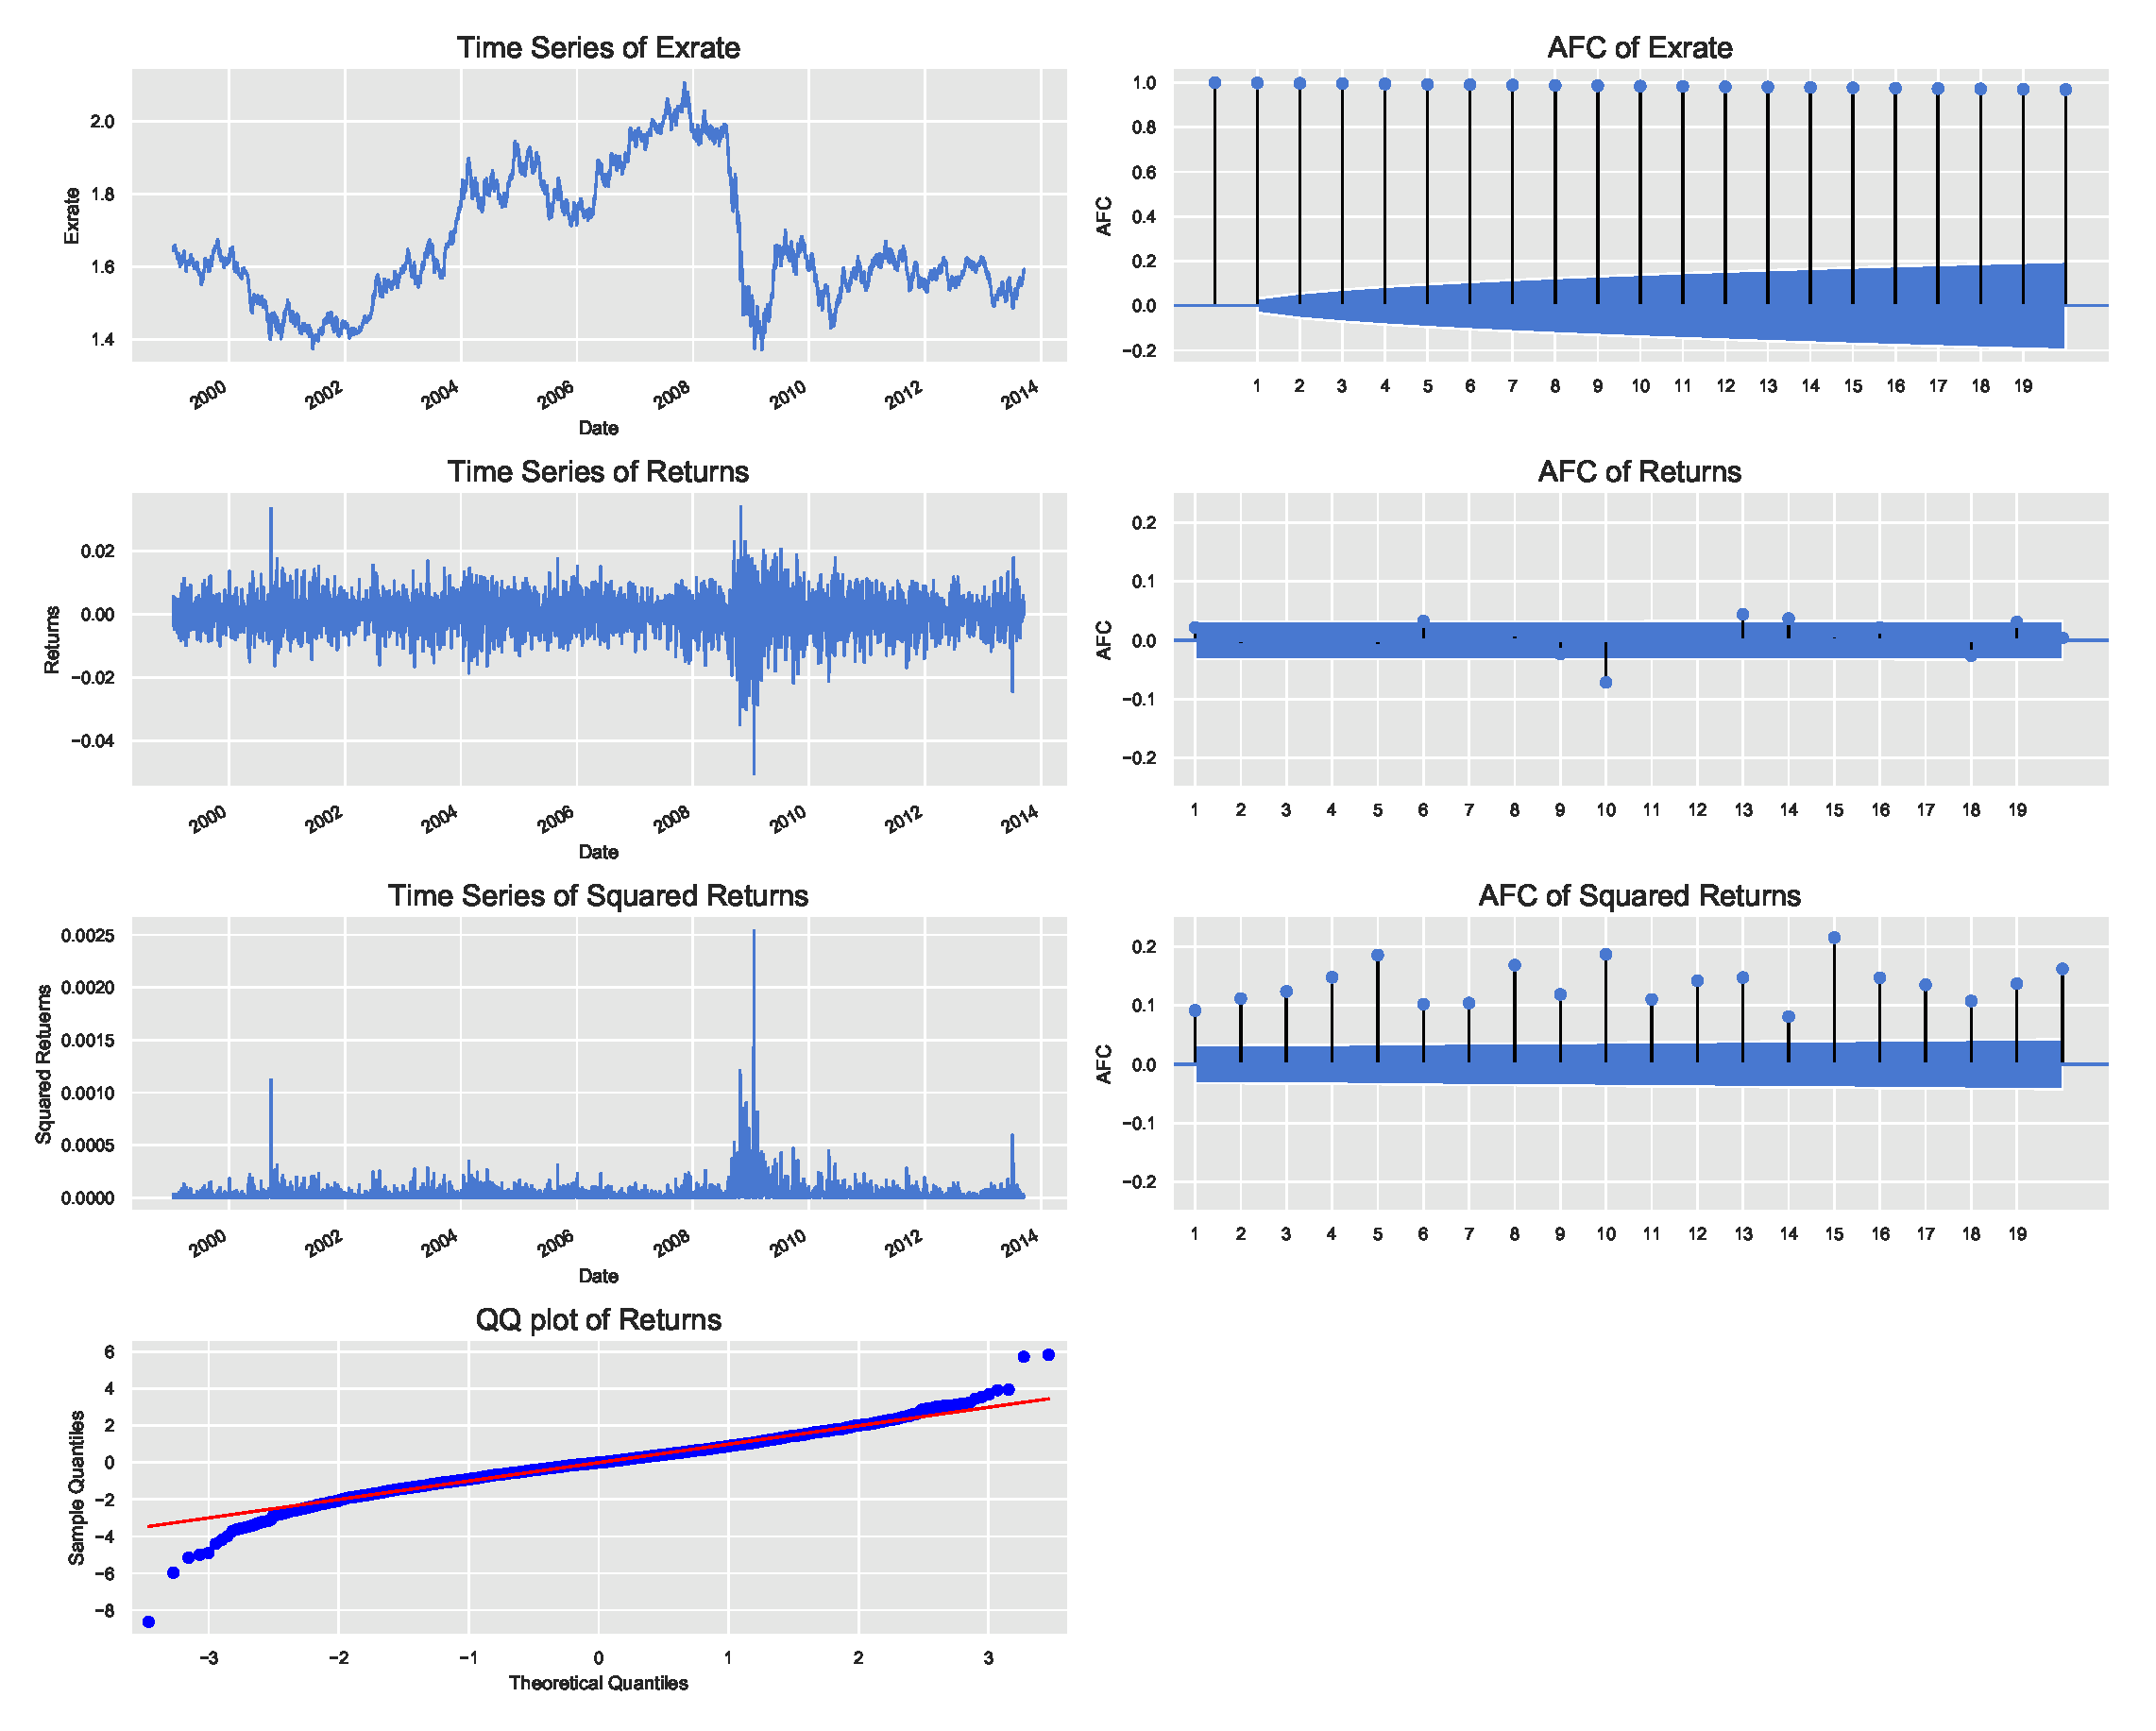
\includegraphics[width=\textwidth]{chapters/chapter_uvts/figures/31graphs.eps}
	\caption{Exchange rate related plots. \label{fig:exchrate}}
	\end{figure}

	\begin{figure}[!ht]
	\centering
	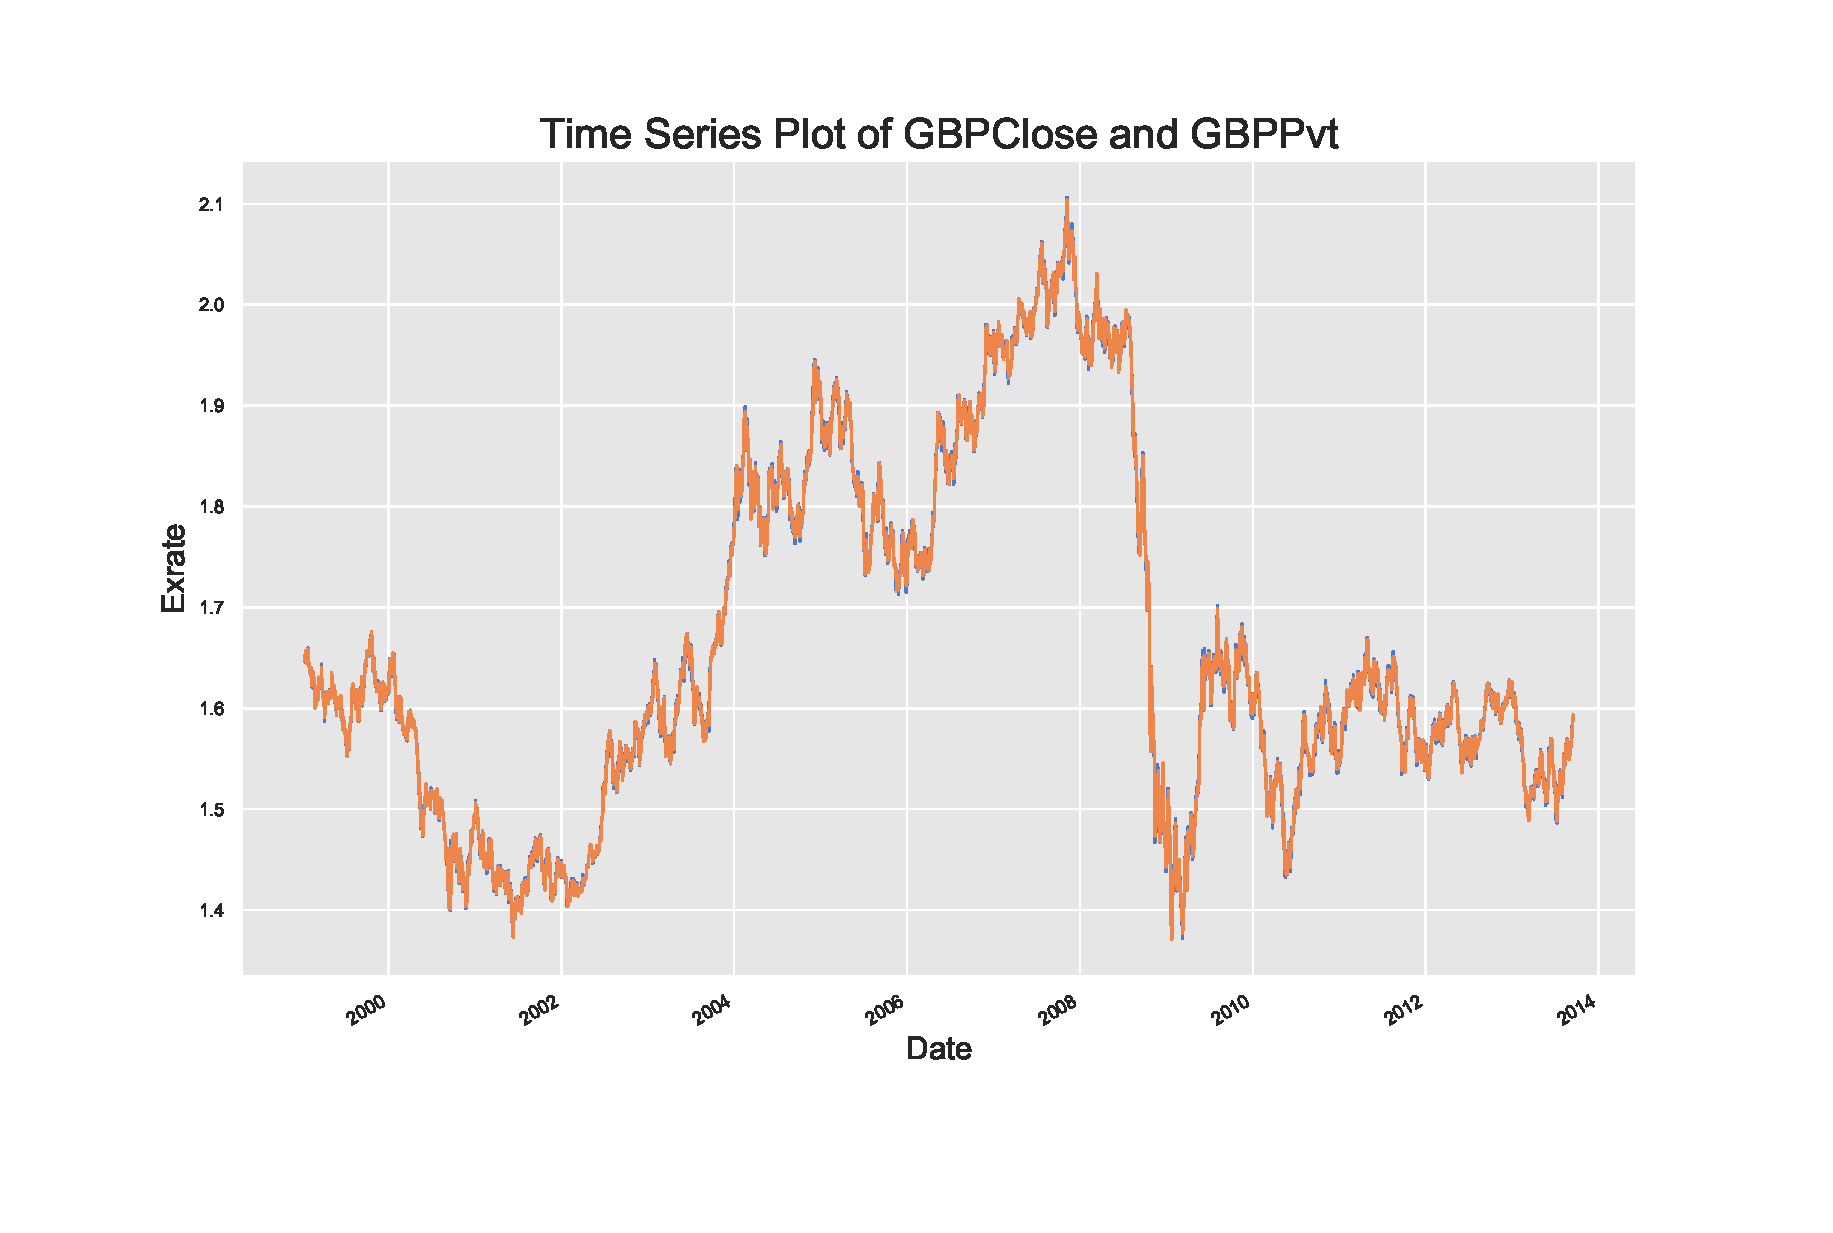
\includegraphics[width=\textwidth]{chapters/chapter_uvts/figures/Sec2-4Fig4.eps}
	\caption{Times series plot of GBPClose, GBPPvt. \label{fig:timegbp}}
	\end{figure}
	
	\begin{figure}[!ht]
	\centering
	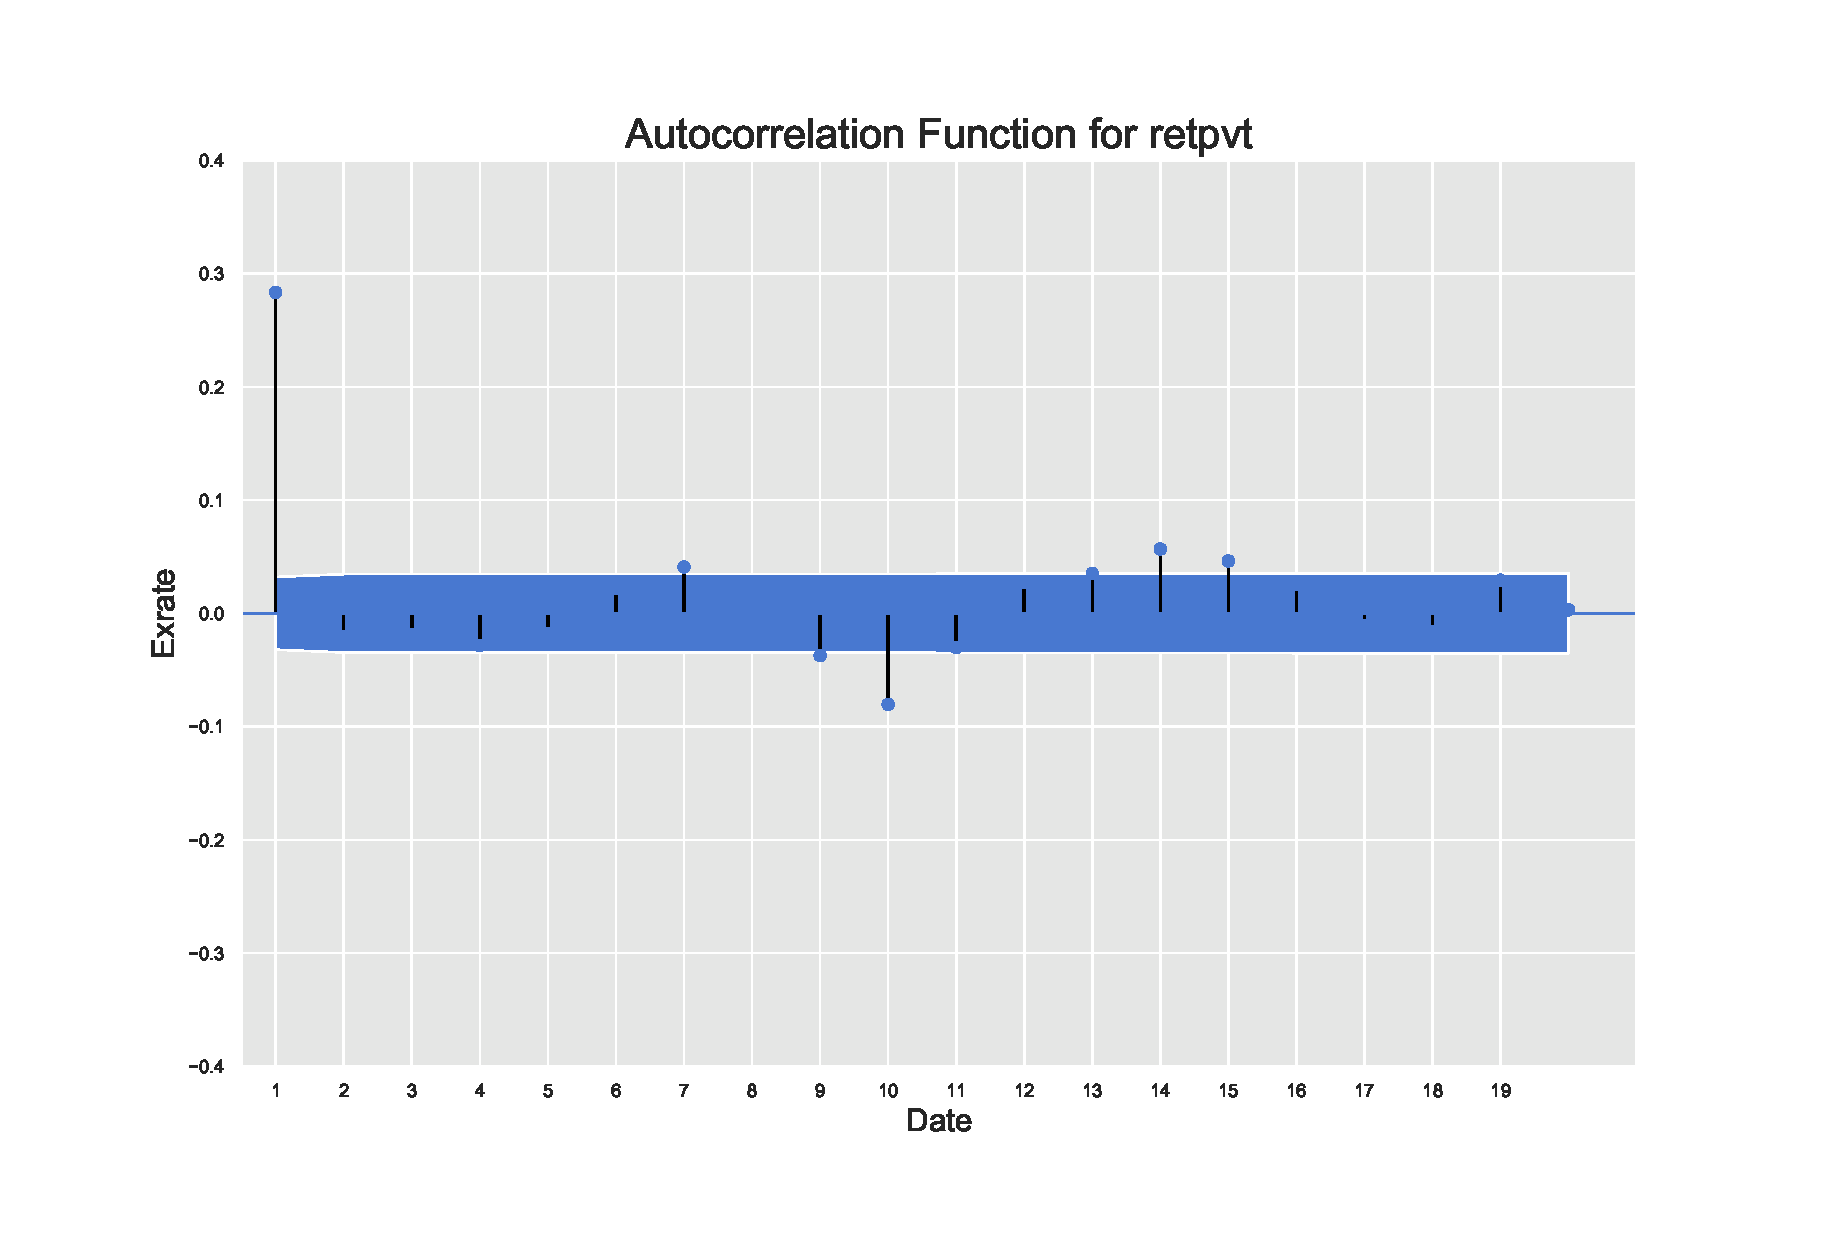
\includegraphics[width=\textwidth]{chapters/chapter_uvts/figures/Sec2-4Fig5.eps}
	\caption{Autocorrelation function for rtpvt. \label{fig:autocorrtpvt}}
	\end{figure}
An assumption of the random walk model that is often made is that the errors (returns)
follow a normal distribution. But in practice, the errors (or returns) tend to have heavier tails than the normal. We suggest using the quantile-quantile plot which is quite sensitive to even modest deviations from normality and also a test based on the properties of normal distribution. An omnibus test based on the skewness ($=0$ for normal) and the kurtosis ($=3$ for normal) is Jarque-Bera test:
	\begin{equation} \label{eqn:2JB}
	\text{JB }= n \left( \frac{\widehat{\text{SK}}^2}{6} + \frac{(\hat{K} - 3)^2}{24} \right) \sim \chi_2^2,
	\end{equation}
where $\text{SK} \text{(ewness)}= \Ex( \frac{X-\mu}{\sigma} )^3, \text{K} \text{(urtosis)} = \Ex( \frac{X-\mu}{\sigma} )^4$. The corresponding sample numbers are substituted in JB (see Jarque and Bera (1980)~\cite{jarque80}). Alternatively, the probability (Q--Q) plot of $r_t = \ln{(p_t)} - \ln{(p_{t-1})}$ as given in Figure~\ref{fig:exchrate} clearly indicates that the distribution has somewhat heavy tails. (For this data $\widehat{SK} = -0.31$ and $\hat{K} = 3.67$ resulting in $\text{JB}= 129.7$ with $n= 3236$, thus rejecting the normal distribution.) \twomedskip


\noindent\textbf{Stylized fact 2:} Heavy Tails: The returns are likely to display a heavy
tailed distribution such as a power-law or Pareto. \twomedskip


\noindent\textbf{Stylized fact 3:} Asymmetry: When prices fall, they tend to fall faster
than when they tend to rise, thus drawdowns tend to be larger than upward rises. \twomedskip

\noindent\textbf{Stylized fact 4:} Positive Excess Kurtosis: Returns generally exhibit high values for the fourth moment due to different phases of high and low trading activity. \twomedskip


These stylized facts are particularly important for risk management of strategies, and how they should be optimally incorporated in trading decisions is still a subject of much research which will be discussed later. The thicker tail distribution warrants that the chance of extreme values are more likely to occur than what is predicted by a normal distribution and the asymmetry indicates that there is a difference between positive and negative sides of variance (volatility). \label{in:assetret2} \label{in:style2}



% Time Series Models for Aggregated Data
\section{Time Series Models for Aggregated Data: Modeling the Variance} \label{in:modelvar1}

In the ARMA$(p,q)$ model $\phi(B)Y_t= \delta + \theta(B) \,\varepsilon_t$ for series $\{ Y_t \}$, when the errors $\varepsilon_t$ are \emph{independent} r.v.'s (with the usual assumptions of zero mean and constant variance $\sigma^2$), an implication is that the \textit{conditional} variance of $\varepsilon_t$ given the past information is a constant not depending on the past. This, in turn, implies the same feature for $l$-step ahead forecast errors $e_t(l) = \sum_{i=0}^{l-1} \psi_i \varepsilon_{t+l-i}$. However, in some settings, particularly for financial data, the variability of errors may exhibit dependence on the past variability. Modeling the variance, which is essential for studying the risk-return relationship is an important topic in finance. \twomedskip


\noindent \textbf{Autoregressive Conditional Heteroscedastic (ARCH) Models} \label{in:arch} \twomedskip


The autoregressive conditional heteroscedastic (ARCH) models were originally proposed by Engle (1982)~\cite{engle1982}, Engle and Kraft (1983)~\cite{engle1983}, to allow for the conditional error variance in an ARMA process to depend on the past squared innovations, rather than be a constant as in ARMA models with independent errors. For example, an AR$(p)$ process with ARCH$(q)$ model errors is given as $Y_t = \sum_{i=1}^p\phi_iY_{t-i} + \delta + \varepsilon_t$, where, $\Ex(\varepsilon_t \;|\; \varepsilon_{t-1},\varepsilon_{t-2},\ldots)= 0$ and \label{in:modelvar2}
	\begin{equation} \label{eqn:2ht}
	h_t= \var(\varepsilon_t \;|\; \varepsilon_{t-1}, \varepsilon_{t-2}, \ldots) = \omega_0 + \sum_{i=1}^q \omega_i \varepsilon_{t-i}^2
	\end{equation}
with $\omega_0 > 0$ and $\omega_i \geq 0$ for $i= 1, \ldots, q$. In the generalized ARCH (GARCH) model, introduced by Bollerslev (1986)~\cite{bollerslev1986}, it is assumed that
	\begin{equation} \label{eqn:2secondht}
	h_t = \omega_0 + \sum_{i=1}^q \omega_i \varepsilon_{t-i}^2 + \sum_{i=1}^k \beta_i h_{t-i},
	\end{equation}
where $\beta_i \geq 0$ for all $i = 1,\ldots,k$. Much subsequent research on and applications of the ARCH and GARCH models have occurred since the publication of their research papers. It is not possible to cover the range of applications resulted from this research here, but these results are widely available to the curious reader.


Let us briefly discuss some basic results and implications of the ARCH and GARCH models.\label{in:garch_model} The errors $\varepsilon_t$ in the model have zero mean, since $\Ex(\varepsilon_t) = \Ex[\Ex(\varepsilon_t \;|\; \varepsilon_{t-1} \ldots)] = 0$, and they are serially uncorrelated; that is, $\Ex(\varepsilon_t \varepsilon_{t-j}) = 0$ for $j \not= 0$ (since for $j > 0$, for example, $\Ex(\varepsilon_t \varepsilon_{t-j}) = \Ex[\Ex(\varepsilon_t \varepsilon_{t-j} \;|\; \varepsilon_{t-1} \ldots)] = \Ex[\varepsilon_{t-j} \Ex(\varepsilon_t \;|\; \varepsilon_{t-1} \ldots)] = 0$). But the $\varepsilon_t$ are not mutually independent r.v.'s since they are inter-related through their conditional variances (i.e., their second moment). We will also assume that the $\varepsilon_t$ have equal unconditional variances, $\var(\varepsilon_t) = \sigma^2$, for all $t$, so they are weakly stationary. Consider then, the simple case of the first-order ARCH or ARCH(1) model,
	\begin{equation} \label{eqn:2htE}
	h_t = \omega_0 + \omega_1 \varepsilon_{t-1}^2,
	\end{equation}
Assuming that $\omega_1 < 1$ ($\omega_0$ and $\omega_1 \geq 0$ is always assumed), the \emph{unconditional} variance of $\varepsilon_t$ is $\sigma^2= \var(\varepsilon_t) = \frac{\omega_0}{1 - \omega_1}$, since $\sigma^2 = \Ex(\varepsilon_t^2) = \Ex[\Ex(\varepsilon_t^2 \,|\, \varepsilon_{t-1}, \ldots)] = \Ex[\omega_0 + \omega_1\varepsilon_{t-1}^2] = \omega_0 + \omega_1\sigma^2$. Therefore, the conditional variance of $\varepsilon_t$ can be written as
	\begin{equation} \label{eqn:2htw}
	h_t = \omega_0 + \omega_1 \varepsilon_{t-1}^2 = \sigma^2 + \omega_1 (\varepsilon_{t-1}^2 - \sigma^2),
	\end{equation}
or in the form of deviation from the unconditional variance as $h_t - \sigma^2= \omega_1 (\varepsilon_{t-1}^2 - \sigma^2)$. So the conditional variance will be above the unconditional variance whenever $\varepsilon_{t-1}^2$ exceeds its unconditional variance $\sigma^2$. If $\varepsilon_t$ were conditionally normally distributed, given the past, the fourth unconditional moment $\Ex(\varepsilon_t^4)$ will exceed $3 \sigma^4$ (the value in the normal distribution), so that the marginal distribution of $\varepsilon_t$ will exhibit fatter tails that the normal distribution. Conditional variances of multi-step ahead forecast errors can also be established to depend on the past squared errors. 


These basic results indicate that the properties of the ARCH(1) model also tend to hold for the higher order ARCH$(q)$ models. A basic impact of the ARCH errors in a process is an assessment of the accuracy of forecast, since the forecast errors will have conditional variances that depend on the past. This allows for formation of correct and more informative (conditional) prediction intervals than that would be obtained under the usual assumption that conditional error variances were constant independent of the past.


Now consider briefly the popular GARCH(1,1) model, $h_t = \Ex(\varepsilon_t^2 \;|\; \varepsilon_{t-1}, \ldots) = \omega_0 + \omega_1\varepsilon_{t-1}^2 + \beta_1h_{t-1}$. Similar to the result for the ARCH(1) model, assuming that $\omega_1 + \beta_1 < 1$, it is readily shown that the unconditional variance of $\varepsilon_t$ is equal to $\sigma^2 = \var(\varepsilon_t) = \omega_0/[1 - (\omega_1 + \beta_1)]$. Let $v_t = \varepsilon_t^2 - h_t$, so that the random variables $v_t$ have zero mean, and they are serially uncorrelated since
	\[
	E\big( (\varepsilon_t^2 - h_t) (\varepsilon_{t-j}^2 - h_{t-j}) \big)= \Ex[(\varepsilon_{t-j}^2 - h_{t-j}) E\{(\varepsilon_t^2 - h_t) \,|\, \varepsilon_{t-1},\ldots\}] = 0.
	\]
Then, since $h_t = \varepsilon_t^2 - v_t$, note that the GARCH(1,1) model can be rearranged as $\varepsilon_t^2 - v_t = \omega_0 + \omega_1\varepsilon_{t-1}^2 + \beta_1(\varepsilon_{t-1}^2 - v_{t-1})$, or
	\begin{equation} \label{eqn:2ept}
	\varepsilon_t^2 = \omega_0 + (\omega_1 + \beta_1)\ \varepsilon_{t-1}^2 + v_t - \beta_1v_{t-1}.
	\end{equation}
This form reveals that the process of squared errors, $\{\varepsilon_t^2\}$, follows an ARMA(1,1) model with uncorrelated innovations $v_t$; however, the $v_t$ are conditionally heteroscedastic. Although this process looks like a linear process, it is not, since $ \{ v_t \}$ are uncorrelated but dependent. This fact motivates the use of the ACF and PACF of the squares $\varepsilon_t^2$ for model specification and for basic preliminary checking for the presence of ARCH/GARCH effects in the errors $\varepsilon_t$. In practice, a starting point would be examination of the sample ACF and PACF of the squared residuals $\hat{\varepsilon}_t^2$, where $\hat{\varepsilon}_t$ are residuals obtained from fitting of a usual ARMA$(p,q)$ model. The correspondence between ARCH and ARMA is further noted via the condition, $0 < \sum_{i=1}^q \omega_i < 1$, that implies the roots of its characteristic equation lie outside the unit circle (like a causal ARMA).


As there are other excellent sources to learn about ARCH and GARCH models (see Tsay (2010)~\cite{tsay}, Chapter~\ref{ch:ch_uvts}), we have limited our discussion to some basic details. For maximum likelihood (ML) estimation of models with ARCH or GARCH errors, refer to Engle (1982)~\cite{engle1982} and Weiss (1984)~\cite{weiss1984}, among others. \twomedskip


\noindent\textbf{Preliminary Testing for ARCH Effect:} This is an omnibus test that examines the presence of autocorrelation up to certain number of lags, which is equivalent to testing, $H_0: \alpha_1 = \alpha_2= \cdots = \alpha_q = 0$ in the model
	\begin{equation} \label{eqn:2eptsq}
	\varepsilon_t^2 = \alpha_0 + \alpha_1 \varepsilon_{t-1}^2 + \cdots + \alpha_q \varepsilon_{t-q}^2 + a_t,
	\end{equation}
where $a_t$ is white noise series; note that $\{ a_t \}$ does not need to follow a normal distribution. The usual $F$-test used in regression can be applied here; Let $R^2$ be the coefficient of determination that results from \eqref{eqn:2eptsq} when $\hat{\varepsilon}_t$'s are used; then
	\begin{equation} \label{eqn:2F}
	F = \frac{R^2/q}{(1 - R^2)/(T - 2q - 1)} \sim \chi^2/q.
	\end{equation}
We use $\chi^2$ instead of $F$ due to the fact that $\varepsilon_t$'s are estimated quantities. More informally, one could use the ACF of $\hat{\varepsilon}_t^2$ and if any of the autocorrelations are out of the normal bounds, $\pm 2/\sqrt{T}$, we may examine further for ARCH effects. \twomedskip


\noindent\textbf{GARCH vs ARCH:} While ARCH models care for the time dependence in volatilities and have elegant properties such as having excessive kurtosis (matching the empirical finding related to asset returns), they tend to overpredict the volatility and treat both negative and positive, $\varepsilon_t$'s symmetrically. To overcome some of these issues and as well as to come up with a more parsimonious representation (as in AR vs ARMA considerations) GARCH models stated in \eqref{eqn:2ept} are proposed. \twomedskip


\noindent\textbf{IGARCH:} The variance can persist for extended periods and can change at different time spans, thus leading to non-stationary behavior. In the GARCH(1,1) model, it is possible that $w_1 + \beta_1 = 1$, so that IGARCH(1,1) (Integrated GARCH) can be written as
	\begin{equation} \label{eqn:2eptsqrt}
	\varepsilon_t = \sqrt{h_t} \cdot a_t, \quad h_t = w_0 + w_1h_{t-1} + (1 - w_1)\ \varepsilon_{t-1}^2.
	\end{equation}
If $h_t$ is proxied by $\varepsilon_t^2$, the above model leads to $\varepsilon_t^2 - \varepsilon_{t-1}^2 = w_0 + w_1(\varepsilon_{t-1}^2 - \varepsilon_{t-2}^2)$, which is similar in form to non-stationary autoregressive model. In practice because of frequent level shifts in volatility, IGARCH appears to be a natural model to fit. Because the IGARCH(1,1) is similar to ARIMA(0,1,1), the model can be taken as an exponential smoothing model for the $\varepsilon_t^2$ series; By iterative substitutions, we can show that
	\begin{equation} \label{eqn:2ht1w}
	h_t = (1 - w_1) \big( \varepsilon_{t-1}^2 + w_1 \varepsilon_{t-2}^2 + w_1^2 \varepsilon_{t-3}^2 \cdots \big),
	\end{equation}
where $w_1$ can be taken as a discount factor. \twomedskip


\noindent\textbf{Prediction Performance of GARCH:} \label{in:forecast2} The predictive power of GARCH based on ex-post forecast evaluation criteria tend to suggest that the model provides poor forecasts, although the in-sample parameter estimates turn out to be highly significant. As Andersen and Bollerslev (1998)~\cite{andersen1998} note, in the model \eqref{eqn:2ept}, the latent volatility, $h_t$, evolves over time. The approach to evaluate the performance of the model for $h_t$ via $\hat{\varepsilon}_t^2$ is not appropriate. While $\hat{\varepsilon}_t^2$ provides an unbiased estimate of $h_t$, it is a noisy measurement due to idiosyncratic error terms associated with it; these error terms may be due to the result of compounding frictions in the trading process. This will be further clarified when we discuss the analysis of high frequency data. \twomedskip


\noindent \textbf{Time--Varying ARCH Processes (tvARCH)} \label{in:tvarch} \twomedskip


The underlying assumptions of ARCH models is stationarity and with changing pace of economic conditions, the assumption of stationarity is not appropriate for modeling financial returns over long intervals. We may obtain a better fit by relaxing the assumption of stationarity in all the time series models. It is also appropriate for building models with local variations. Dahlhaus and Subba Rao (2006)~\cite{dahlhaus2006} generalize the ARCH model with time-varying parameters:
	\begin{equation} \label{eqn:2eptsqrtht}
	\varepsilon_t = \sqrt{h_t}\cdot a_t, \quad h_t = w_0(t) + \sum_{j=1}^{\infty} w_j(t) \varepsilon_{t-j}^2,
	\end{equation}
which $a_t$'s are i.i.d. with mean zero and variance, one. By rescaling the parameters to unit intervals, the tvARCH process can be approximated by a stationary ARCH process. A broad class of models resulting from \eqref{eqn:2eptsqrtht} can be stated as:
	\begin{equation} \label{eqn:2eptN}
	\varepsilon_{t,N} = \sqrt{h_{t,N}} \cdot a_t, \quad h_{t,N} = w_0 \left( \frac{t}{N} \right) + \sum_{j=1}^pw_j \left (\frac{t}{N} \right) \varepsilon_{t-j,N}^2
	\end{equation}
for $t= 1, 2, \ldots, N$. This model captures the slow decay of the sample autocorrelations in squared returns that is commonly observed in financial data which is attributed to the long memory of the underlying process. But tvARCH$(p)$ is a non-stationary process that captures the property of long memory.


Fryzlewicz, Sapatinas and Subba Rao (2008)~\cite{fryzlewicz2008} propose a kernel normalized-least squares estimator which is easy to compute and is shown to have good performance properties. Rewriting \eqref{eqn:2eptN} as
	\begin{equation} \label{eqn:2eptNsq}
	\varepsilon_{t,N}^2 = w_0 \left(\frac{t}{N}\right) + \sum_{j=1}^p w_j \left(\frac{t}{N}\right)\varepsilon_{t-j,N}^2 + (a_t^2 - 1)h_{t,N}^2
	\end{equation}
in the autoregressive form, the least squares criterion with the weight function, $k(u_0,\chi_{k-1,N})$, where $\chi_{k-1,N}' = (1,\varepsilon_{k-1,N}^2, \ldots, \varepsilon_{k-p,N}^2)$ is
	\begin{equation} \label{eqn:2Lt0}
	L_{t_0,N}(\alpha) = \sum_{k=p+1}^N \frac{1}{b_N} \;w \left(\frac{t_0-k}{b_N} \right) \frac{\left(\varepsilon_{k\cdot N}^2 - \alpha_0 - \sum_{j=1}^p \alpha_j \varepsilon_{k-j \cdot N}^2 \right)^2}{k(u_0, \chi_{k-1\cdot N})^2}.
	\end{equation}
Minimizing \eqref{eqn:2Lt0} yields, $\hat{a}_{t_0,N} = R_{t_0,N}^{-1} r_{t_0,N}$, where
	\begin{flalign} \label{eqn:2Rt0}
	&& R_{t_0,N}&= \sum_{k=p+1}^N \frac{1}{b_N}\ ; w \left(\frac{t_0-k}{b_N} \right) \frac{\chi_{k-1\cdot N} \chi_{k-1\cdot N}'}{k(u_0, \chi_{k-1\cdot N})^2} && \notag \\
	\text{and} && \phantom{x} & \phantom{x} && \\
	&& r_{t_0,N} &= \sum_{k=p+1}^N \frac{1}{b_N}\; w \left(\frac{t_0-k}{b_N}\right)\frac{\varepsilon_{k\cdot N}^2  \chi_{k-1\cdot N}}{k(u_0,\chi_{k-1\cdot N})^2}. && \notag
	\end{flalign}
The kernel $w$ is a function defined on $[-\frac{1}{2},\frac{1}{2}]$ which is of bounded variation. The choice of weight function suggested is as follows: it is motivated by the differing variances at various values of $k$. Estimate,
	\begin{flalign} \label{eqn:2skN}
	&& \hat{\mu}_{t_0,N}&= \sum_{k=1}^N\frac{1}{b_N} \; w\left(\frac{t_0 - k}{b_N}\right)\varepsilon_{k\cdot N}^2 && \notag \\
	\text{and} && \phantom{x} & \phantom{x} && \\
	&& s_{k-1\cdot N} &= \sum_{j=1}^p\varepsilon_{k-j\cdot N}^2 && \notag
	\end{flalign}
and use $k_{t_0,N}(s_{k-1},N) = \hat{\mu}_{t_0,N} + s_{k-1\cdot N}$ as the weight function. Thus the estimation is a two-stage scheme. For the bandwidth selection, the cross-validation method based on a subsample of the observations is suggested.


The methodology presented here is useful because of the changing nature of financial volatility. Real data applications will be discussed in Chapter~\ref{ch:stat_ts}. Here the volatility at the low frequency level is estimated by $r_t^2$, where $r_t$, the returns is based on closing prices of successive days. Alternative approaches to estimating volatility using aggregate prices bars or high frequency data will be discussed in Chapter~\ref{ch:ch_advanced}. 



% Stylized Models for Variance of Asset Returns
\section{Stylized Models for Variance of Asset Returns \label{sec:sty_mod_var}} \label{in:assetvol1} \label{in:style3}

Volatility has many important implications in finance. It is one of the most commonly used risk measure and plays a vital role in asset allocation. The estimate of volatility of an asset is obtained using the prices of stock or options or both. Three different measures that are normally studied are stated below:


\begin{itemize}
\item Volatility is the conditional standard deviation of daily or low frequency returns.
\item Implied volatility is derived from options price under some assumed relationship between the options and the underlying stock prices.
\item Realized volatility is an estimate of daily volatility using high frequency intraday returns.
\end{itemize}


In this section, we will mainly focus on the first item and the others will be discussed in a later section on high frequency data.


Consider $r_t = \ln{(p_t) - \ln{(p_{t-1})}}$, return of an asset. We observed that `$r_t$' exhibits no serial correlation. This does not imply that the series `$r_t$' consists of independent observations. The plot of $r_t^2$ given in Figure~\ref{fig:exchrate} clearly indicates that volatility tends to cluster over certain time spans. The autocorrelations in Figure~\ref{fig:exchrate} confirms that there is some time dependence for the volatility. In fact in some cases, there is some long range dependence that spans up to sixty days. \twomedskip


\noindent\textbf{Stylized fact 5:} Volatility clustering: \label{in:volclust1} High volatility events tend to cluster in time and this can be measured through positive correlations that exist over several lags.


To formally model the volatility, recall the conditional mean and the conditional variance of the return, $r_t$, are: $\mu_t = \Ex(r_t \;|\; F_{t-1})$, $\sigma_t^2 = \var(r_t \;|\; F_{t-1}) = \Ex( (r_t - \mu_t)^2 \;|\; F_{t-1})$. We have observed for the exchange rate series that $\mu_t \approx$ constant and is generally close to zero. But $\sigma_t^2$ clusters around certain time spans and modeling variation in $\sigma_t^2$ is typically done through ARCH/GARCH models and also through stochastic volatility models. The stochastic volatility models have the advantage of modeling jumps in prices that are also often used in derivative pricing. To begin with, we can test for the heteroscedasticity using the test in \eqref{eqn:2F} or one of the following which are all equivalent asymptotically: \label{in:assetvol2} \label{in:style4}


\begin{itemize}
\item \textbf{Ljung-Box Omnibus Test:}
	\begin{equation} \label{eqn:2Qk}
	Q_k = T(T+2) \cdot \sum_{j=1}^k\frac{(\hat{e}^{j})^2}{T - j} \sim \chi_{k-m}^2,
	\end{equation}
where $\hat{e}^{(j)}$ is the $j$th lag autocorrelation of $r_t^2$; $m$ is the number of independent parameters. Here we test the null hypothesis, $H_0: \rho_1 = \rho_2 = \cdots \rho_k = 0$.

\item \textbf{Lagrange Multiplier Test:} Regress $r_t^2$ on $r_{t-1}^2, \ldots, r_{t-q}^2$ and obtain $R^2$ the coefficient of determination; Test the $H_0$: Slope coefficients are all zero, by
	\begin{equation} \label{eqn:2TstarR}
	T \cdot R^2 \sim \chi_q^2.
	\end{equation}
\end{itemize}


These tests were carried out on the exchange rate data; Table~\ref{tab:box} has the result of Ljung-Box Test: 
        \begin{table}[!ht]
        \centering
        \caption{Ljung-Box Chi-Square Statistics for Exchange rate data \label{tab:box}}
        	\begin{tabular}{ccccc}
        	 h & 12 & 24 & 36 & 48 \\ \hline
        	$Q_h$ & 73.2 & 225.7 & 463.4 & 575.7 \\ \hline
        	df & 6 & 18 & 30 & 42 \\ \hline
        	$p$-value & 0.000 & 0.000 & 0.000 & 0.000 \\
        \end{tabular}
        \end{table}


The Lagrange Multiplier test with $q=5$ also gives $R^2= 0.065$, that $T \cdot R^2 = 243.6$ and compared with $\chi_5^2$ table values has $p$-value $\approx$ 0. These results clearly confirm that there is some time dependence in the volatility.


Among the conditional heteroscedasticity models ARCH/GARCH that were discussed in the last section, GARCH is simple to use and also results in more parsimonious modeling. Therefore, we present only the estimated GARCH model here. For exchange rate data, the estimated GARCH model is $\hat{\sigma}_t^2 = 2.61 \times 10^{-7} + 0.037r_{t-1}^2 + 0.95\hat{\sigma}_{t-1}^2$. Observe that the coefficients $r_{t-1}^2$ and $\hat{\sigma}_{t-1}^2$ add up to unity approximately and thus indicating the volatility is best modeled through IGARCH, which seems to hold generally for many asset volatilities.



% Exercises
\section{Exercises\label{sec:three_exercise}}


% Problem
\prob Consider the exchange rate daily data from December 4, 2006 to November 5, 2010 (Rupee versus Dollar, Pound and Euro), Rates.csv.

\begin{enumerate}[(a)]
\item Compute the sample average, standard deviation and the first order autocorrelation of daily returns over the entire sample period.  Test if the mean and the first order autocorrelation are significantly different from zero using the tests proposed in Section~\ref{sec:key_step}. 
\item Plot histograms of the returns over the entire sample period; Does the distribution look normal?  Test it through Jarque-Bera test in \eqref{eqn:2JB}.
\item Aggregate the data at the weekly level; do (a) and (b) on the aggregated data. Compare the result with the result for the daily level. \twomedskip
\end{enumerate}


% Problem
\prob For the returns of all three time series in Problem~1,  construct\dots

\begin{enumerate}[(a)]
\item ARMA models for the returns; identify the model structure via ACF and PACF.
\item  GARCH models for the squared returns; compare the model coefficients for the three series.  Comment on the difference, if any.
\item Is there a co-movement among the three exchange-rate series? To make the plots on a comparable scale, convert the starting points of the series unity. Does the co-movement vary over different time regimes? (Back up your claim with solid analysis.) Identify the transition states and speculate how you can exploit this for trading decisions. \twomedskip
\end{enumerate}


% Problem
\prob Exchange Rates: The file \texttt{Exchange Rates.csv} contains exchange rates between US dollar and twenty-five major currencies. The daily data spans from Jan 3, 2000 to April 10, 2012. Use this data to perform the following tasks: after computing the returns, $r_t=\log(p_t)-\log(p_{t-1})$ for each series.

\begin{enumerate}[(a)]
\item Plot histograms of the returns and test if the distributions are normal, via Q--Q plots.
\item Compute the auto-correlation function and identify which lags are significant. What is the tentative ARMA model?
\item Is there any ARCH effect? Why?
\item Fit GARCH(1,1) and IGARCH(1,1) models using both normal and $t$-distributions for the innovations. Which volatility model appears to be the best? \twomedskip
\end{enumerate}


% Problem
\prob Exchange rates: Consider the original series, $p_t$, for the duration starting June 11, 2003.
 Answer the following after dividing each series by $p_1$, so that the starting points are the same.
 
\begin{enumerate}[(a)]
\item Identify for each series, if there are any regime changes. Test if these changes are statistically significant.
\item Identify how many clusters are there and if the membership changes under different regimes.
\item Do the series move together? Provide some intuitive tests (more formal tests will be covered in Chapter~\ref{ch:ch_mvts}). 
\item Compare the results in (c) with (b). What is the connection between clustering and co-movement? Briefly discuss. \twomedskip
\end{enumerate}


% Problem
\prob Consider daily price of Apple stock from January 2, 2015 to January 2, 2018. The data can be obtained from Yahoo Finance and have 7 columns (namely, Date, Open, High, Low, Close, Volume, Adj Close). We focus on the adjusted closing price in the last column.

\begin{enumerate}[(a)]
\item Compute the daily log returns. Is there any serial correlation in the daily log returns? Use the test for white noise as outlined in the text. 
\item Consider the pivot based on the pivot based on the average of high and low price and the pivot based on the average of high, low and close prices. Compute the returns based on the pivot log prices and test for serial correlation. Compare this result with the finding in (a). 
\item Consider the log price series of AAPL stock. Is the log price series unit-root non-stationary? Perform a unit-root (Dickey-Fuller) test to answer the question and present your conclusion. \twomedskip
\end{enumerate}


% Problem
\prob Consider daily price of Apple stock again.
\begin{enumerate}[(a)]
\item Compute various measures of variance computed from the entries of the price bars. Comment on their correlation with log volume. 
\item Use the ARIMA modeling to come up with a parsimonious model for log volume. Comment on the model accuracy by setting aside a validation data set. \twomedskip
\end{enumerate}


% Problem
\prob The \textit{Roll} model for trade prices discussed in the text can be more specifically stated as,
	\[
	\begin{aligned}
	p_t^*&= p_{t-1} + \epsilon_t, \;\;\;\;\; \epsilon_t \sim N(0,\sigma^2) \;\;\text{and} \\
	p_t&= p_t^* + c s_t, \;\;\;\;\; \text{where }s_t \in \{+1,-1\}
	\end{aligned}
	\]
Here $p_t^*$ is the ``true'' value of a security and $p_t$ is the observed trade price, which differ because of the bid-offer spread: $c$ is the half-spread and $s_t$ is the direction of the $t$th trade. $s_t$ and $\epsilon$ are serially independent and independent of each other.
\begin{enumerate}[(a)]
\item Calculate the serial correlation of the observed prices $p_t$. Construct an MA(1) model with the same autocorrelation structure. Of the two such models, take the invertible one. 
\item For the invertible model, construct the associated AR model. 
\item Use the model to show how to estimate the bid-ask spread and apply the results on the Apple data used in Problems 5 and 6. \twomedskip
\end{enumerate}


% Problem
\prob Consider the Level~III data for the ticker, ``BIOF'' for a single day. The data description follows the similar details as given in Table~\ref{tab:CISCO}. This exercises consists of two parts; in the first part, we want to construct the limit order book and the second part we want to study the effect of time aggregation. 

\begin{enumerate}[(a)]
\item At any point in time, a limit-order book contains a number of buy and sell orders.
	\begin{enumerate}[(i)]
	\item Develop a program that can visually present a limit order book. Present the order book diagram as of 11:00~a.m. for the first tern positions on both sides.
	\item Aggregate demand and supply are represented as step functions of shares accumulated at each price level. The height of step `$i$' on the demand side is the price side is the price difference between $(i-1)$th and $i$th best price. The height of the first step is the mid price; the length of a step, `$i$', on the demand side is the total number of shares across all orders until $i$th price. Similarly, the supply side can be constructed. Normalize a step height by the cumulative length from the first step to tenth step. Present the aggregate curve as of 11:00~a.m.
	\item Using the aggregate graph give in (ii), suggest measures for the order book imbalance---which is a key determinant in some entry/exit algorithms in the high-frequency setting.
	\end{enumerate}

\item Aggregate the data to a 2-minute interval, summarizing the number of transactions, volume weighted average price and average duration between transactions. Also, produce the price bars (open, close, low and high and volume) for each interval.
	\begin{enumerate}[(i)]
	\item Briefly discuss how you would quantify the loss of information due to aggregation.
	\item Calculate the variance of the returns based on the aggregated VWAP and compare it with the variance based on all observations.
	\item From Exercise~7, it follows that the true price is measured with error, which is due to market friction. The aggregation done above may cancel out the friction and may reflect the true price. Alternatively, one can sample the price every two minutes and compute the variance in the returns. How does this compare to VWAP based descriptives?
	\end{enumerate}
\end{enumerate}
% !TEX root = ../../exercises.tex
\chapter{Multivariate Time Series Models \label{ch:ch_mvts}}
% !TEX root = ../../book.tex
\chapter{Advanced Topics\label{ch:ch_advanced}}

In this chapter,\label{in:adv_model} we want to discuss some advanced methods that are applicable in the context of trading. The mechanics of actual trading (entry/exit) decisions call for trading the market movements in real time and the tools provided in this chapter would be quite useful to better track and understand the market changes. This chapter is broadly divided into two main areas; the first area covers topics which are extensions of models discussed in Chapter~\ref{ch:ch_uvts} in the low frequency context. Although the state-space modeling is discussed in the context of ARIMA, its scope is much wider. We also outline the established methodology for studying regime switching, but indicate the topics of further research where predicting ahead when the regime shift is likely to occur using signals from the past is of great interest. This is followed by a discussion on using volume information to study the price volatility. With the increased exploitation of price behavior data, it has become necessary to look for additional trading signals. We present a theoretical model that shows that there is correlation between volume traded and volatility when there is information flow. The second area of this chapter focuses on the models from point processes to study the higher frequency data. Here our approach has been to provide an intuitive discussion of main tools; as readers will realize, the trade data is quite noisy due to market friction, The formal parametric models do not perform well. Thus there is a great deal of scope to do research in non-parametric empirical modeling of arrivals and cancellations in the limit order market. 



% State-Space Modeling
\section{State-Space Modeling\label{sec:state_space}}

The state-space models were initially developed by control systems engineers to measure a signal contaminated by noise.\label{in:state_space} The signal at time ``$t$'' is taken to be a linear combination of variables, called state variables that form the so-called state vector at time, $t$. The key property of the state vector is that it contains information from past and present data but the future behavior of the system is independent of the past value and depends only on the present values. Thus the latent state vector evolves according to the Markov property. The state equation is stated as,
	\begin{equation} \label{eqn:2zt}
	Z_t = \Phi_tZ_{t-1} + a_t
	\end{equation}
and observation equation as,
	\begin{equation} \label{eqn:2yt}
	Y_t = H_tZ_t + N_t,
	\end{equation}
where it is assumed that $a_t$ and $N_t$ are independent white-noise processes; $a_t$ is a vector white noise with covariance matrix $\Sigma_a$ and $N_t$ has variance $\sigma_N^2$. The matrix $\Phi_t$ in \eqref{eqn:2zt} is an $r \times r$ transition matrix and $H_t$ in \eqref{eqn:2yt} is a $1 \times r$ vector; both are allowed to vary in time. In engineering applications, the structure of these matrices are governed by some physical phenomena. 


The state space form of an ARIMA$(p,d,q)$ process $\Phi(B)Y_t= \theta(B)\epsilon_t$ has been extensively studied (see Reinsel (2002)~\cite[Section~2.6]{2002reinsel}). Observe if $\Phi_t \equiv \Phi$ and $H_t \equiv H$ for all $t$ then the system \eqref{eqn:2zt}--\eqref{eqn:2yt} is said to be time-invariant. A nice feature of expressing a model in state-space form is that an updating procedure can be readily used when a new observation becomes available to revise the current state vector and to produce forecasts. These forecasts in general tend to fare better. 


For the state-space model, define the finite sample estimates of the state vector $Z_{t+1}$ based on observations $Y_t, \ldots, Y_l$, as $\hat{Z}_{t+l|t} = \Ex[Z_{t+l} \;|\; Y_t,\cdots,Y_l],\text{ with } V_{t+l \;|\; t} = \Ex[(Z_{t+l} - \hat{Z}_{t+l \;|\; t})(Z_{t+l} - \hat{Z}_{t+l \;|\; t})']$. A convenient computational procedure, known as the \emph{Kalman filter equations},\label{in:kalman} is used to obtain the current estimate $\hat{Z}_{t\;|\;t}$, in particular. It is known that (see Reinsel (2002)~\cite{2002reinsel}), starting from some reasonable initial values $Z_0 \equiv \hat{Z}_{0 \;|\; 0}$ and $V_0 \equiv V_{0\;|\;0}$, the estimate, $\hat{Z}_{t \;|\; t}$, can be obtained through the following recursive relations:
	\begin{equation}\label{eqn:2hatz}
	\hat{Z}_{t \;|\; t} = \hat{Z}_{t \;|\; t-1} + K_t(Y_t - H_t \hat{Z}_{t \;|\; t-1}),
	\end{equation}
where $K_t= V_{t \;|\; t-1} H_t'[H_t V_{t \;|\; t-1} H_t' + \sigma_N^2]^{-1}$ with $\hat{Z}_{t \;|\; t-1} = \Phi_t \hat{Z}_{t-1\;|\; t-1},V_{t \;|\; t-1} = \Phi_t V_{t-1\;|\; t-1} \Phi_t' + \Sigma_{a}$ and $V_{t \;|\; t} = [I - K_t H_t] V_{t \;|\; t-1} = V_{t\;|\; t-1} - V_{t\;|\; t-1} H_t' [H_t V_{t \;|\; t-1} H_t' + \sigma_N^2]^{-1} H_t V_{t \;|\; t-1}$ for $t= 1,2, \ldots$.


In \eqref{eqn:2hatz}, the quantity $\varepsilon_{t \;|\; t-1}= Y_t - H_t \hat{Z}_{t \;|\; t-1} \equiv Y_t - \hat{Y}_{t \;|\; t-1}$ at time $t$ is the new information provided by the measurement $Y_t$, which was not available from the previous observed (finite) history of the system. The factor $K_t$ is termed the ``Kalman gain'' matrix. The filtering procedure in \eqref{eqn:2hatz} has the recursive ``updating'' form, and these equations represent the minimum mean square error predictor property. For example, note that $\Ex[Z_t \,|\,Y_t,\ldots,Y_1]= \Ex[Z_t \,|\,Y_{t-1},\cdots,Y_1] + \Ex[Z_t \,|\, Y_t - \hat{Y}_{t \;|\; t-1}]$, since $\varepsilon_{t \;|\; t-1} = Y_t - \hat{Y}_{t \;|\; t-1}$ is independent of $Y_{t-1}, \ldots, Y_1$. Note from \eqref{eqn:2hatz}, the estimate of $Z_t$ equals the prediction of $Z_t$ from observations through time $t-1$ updated by the factor $K_t$ times the innovation $\varepsilon_{t|t-1}$. The quantity $K_t$ can be taken as the regression coefficients of $Z_t$ on the innovation $\varepsilon_{t|t-1}$, with $\var(\varepsilon_{t\;|\; t-1}) = H_t V_{t\;|\; t-1} H_t' + \sigma_N^2$ and $\cov(Z_t,\varepsilon_{t\;|\; t-1})= V_{t \;|\; t-1} H_t'$. Thus, the general \emph{updating relation} is $\hat{Z}_{t\;|\;t} = \hat{Z}_{t\;|\; t-1} + \cov(Z_t,\varepsilon_{t\;|\; t-1}) \{ \var(\varepsilon_{t\;|\; t-1}) \}^{-1} \varepsilon_{t\;|\; t-1}$, where $\varepsilon_{t \;|\; t-1} = Y_t - \hat{Y}_{t\;|\; t-1}$, and the relation in $V_t$ is the usual updating of the error covariance matrix to account for the new information available from the innovation $\varepsilon_{t\;|\; t-1}$. Forecasts of future state values are available as $\hat{Z}_{t+l\;|\;t} = \Phi_{t+l} \hat{Z}_{t+l-1\;|\;t}$ for $l = 1,2,\ldots$. 


Note for ARIMA models with $Y_t = HZ_t$ and $H = [1,0,\ldots,0]$, this Kalman filtering procedure provides an alternate way to obtain finite sample forecasts, based on data $Y_t,Y_{t-1}, \cdots, Y_1$, for future values in the ARIMA process, subject to specification of appropriate initial conditions to use in the terms in \eqref{eqn:2hatz}. For stationary $Y_t$ with $\Ex(Y_t)= 0$, the appropriate initial values are $\hat{Z}_{0 \;|\;0} = 0$, a vector of zeros, and $V_{0 \;|\;0} = \cov(Z_0) \equiv V_*$, the covariance matrix of $Z_0$. Specifically, because the state vector $Z_t$ follows the stationary vector AR(1) model $Z_t = \Phi Z_{t-1} + \psi \varepsilon_t$, its covariance matrix $V_*= \cov(Z_t)$ satisfies $V_*= \Phi V_* \Phi' + \sigma_{\varepsilon}^2 \Psi \Psi'$, which can be readily solved for $V_*$. For nonstationary ARIMA processes, additional assumptions need to be specified. The ``steady-state'' values of the Kalman filtering procedure $l$-step ahead forecasts $\hat{Y}_{t+l\;|\;t}$ and their forecast error variances $v_{t+l\;|\;t}$ will be identical to the expressions given in Chapter~\ref{ch:ch_uvts}, $\hat{Y}_t(l)$ and $\sigma^2(l) = \sigma^2 (1 + \sum_{i=1}^{i-1}\psi_{i}^2 )$. 


An alternative set-up, alternative to is to assume that the deviations in the observation and transition equations are related. With the observation equation stated in \eqref{eqn:2yt}, the transition equation is modified as 
	\begin{equation} \label{eqn:223zt}
	Z_t = \Phi Z_{t-1} + \alpha N_t.
	\end{equation}
This model studied in Ord, Koehler, and Snyder (1997)~\cite{ord1997estimation} with a single source of error $(N_t)$ is shown to be closely related to various exponential smoothing procedures. There are other formulations of state-space models, such as structural models by Harvey (1989)~\cite{harvey1989kalman} and dynamic linear models of West and Harrison (1997)~\cite{west1997} that are found to be useful for model building.


We provide two examples to illustrate the application of the models \eqref{eqn:2zt} and \eqref{eqn:2yt} in the broader context of this book. 


\begin{ex}[Generalized Local Trend]
The slope in a local linear trend is a random walk. Specifically,
	\begin{equation} \label{eqn:randomwalk}
	\begin{aligned}
	p_t&= \mu_t + e_t \\
	\mu_t&= \mu_{t-1} + \delta_{t-1} + \eta_{0t} \\
	\delta_t&= \delta_{t-1} + \eta_{1t}
	\end{aligned}
	\end{equation}
Here the trend is composed of level `$\mu_t$' and slope `$\delta_t$'. The slope `$\delta_t$' when written as 
	\begin{equation} \label{eqn:slopewritten}
	\delta_t= D+ e(\delta_{t-1} - D)+ \eta_{1t}
	\end{equation}
in AR(1) form is sometimes known as generalized local linear trend. These models can be written in the form of \eqref{eqn:2zt} and \eqref{eqn:2yt}; the updating process given in \eqref{eqn:2hatz} can be used to accommodate a wide range of models. \xqed
\end{ex}


\begin{ex}[Price Discovery in Multiple Markets]
Menkveld, Koopman and Lucas (2007)~\cite{menkkoop} study the price discovery process for stocks that are cross-listed in two different markets via state-space models. The question if the trading location matters more than business location is of interest to finance researchers. Consider a stock traded in Amsterdam and in NY exchanges. Because of the time difference, there is only an hour of overlap in trading. Ignoring this aspect, write the two-dimensional price vector as
	\begin{equation}
	\begin{aligned}
	p_t&= \mu_t + e_T \\
	&=\mu_t + \theta(\mu_t - \mu_{t-1}) + e_t
	\end{aligned}
	\end{equation}
as the observational equation with delayed price reaction and the state equation is
	\begin{equation}
	\mu_t= \mu_{t-1} + \xi_t.
	\end{equation}
Here $\epsilon_t$ can represent a more general covariance structure such as the factor model where a common factor that can influence both prices could be easily accommodated. The above can be written in the form of \eqref{eqn:2zt} and \eqref{eqn:2yt} with appropriate choice of `$\Phi$' and `$H$' matrices. For details see Section~2.4 of Menkveld et al. (2007)\cite{menkkoop}. The main advantage of state-space models is that they accommodate the possibility of slowly varying parameters over time, which is more realistic in modeling the real world data. \xqed
\end{ex}


The estimation of model parameters can be done via likelihood function. For this and how VAR models discussed in Chapter~4 can be written in the state-space form, see Reinsel (2002)~\cite{2002reinsel}.



% Regime Switching and Change-Point Models
\section{Regime Switching and Change-Point Models}


It has been long noted in finance that there are two kinds of recurrences in stock prices: underreaction and overreaction to a series of good or bad news.\label{in:regime} The securities that have a good record for an extended period tend to become overpriced and have low returns subsequently. Barberis, Shleifer and Vishny (1998)~\cite{vishny} present a model where investor believes that the returns can arise from one of two regimes although returns follow random walk: mean-reverting or trending. The transition probabilities are taken to be fixed and the regime is more likely to stay the same rather than to switch. But the investor's beliefs are updated as and when the returns data are observed. It is presumed that in many instances, we may not discern these shifts directly whether or when they occur but instead can draw probabilistic inference based on the observed behavior posthumously. Hamilton (2016)~\cite{jdham} reviews the area of regime-switching applied in several contexts in macroeconomics, building upon the elegant model introduced in Hamilton (1989)~\cite{89ham}. Here in this section, we will cover only studies that are relevant to finance applications, particularly relevant to trading that exploit anomalies. 


Consider the model,
	\begin{equation} \label{eqn:modelham}
	y_t = \mu_{s_t} + \epsilon_t, \quad s_t= 1, 2,
	\end{equation} 
where $y_t$ is the observed variable, such as asset return and $s_t$ represents two distinct regimes and $\epsilon_t$'s are i.i.d. $\sim N(0,\sigma^2)$. Let $\{ F_{t-1} \}$ be the information set available as of `$t-1$'. The transition between the regimes is taken to be Markovian,
	\begin{equation} \label{eqn:markprob}
	\text{Prob}(s_t= j \;|\; s_{t-1}= i, F_{t-1}) = p_{ij}, \quad i,j= 1, 2;
	\end{equation}
thus, leading to an AR(1) model for $\mu_{s_t}$ as
	\begin{equation} \label{eqn:must}
	\mu_{s_t} = \phi_0 + \phi_1 \mu_{s_{t-1}} + a_t,
	\end{equation}
where $a_t$ by definition can take four possible values depending upon $s_t$ and $s_{t-1}$. Note $\phi_0= p_{21} \mu_1 + p_{12} \mu_2$ and $\phi_1= p_{11} - p_{21}$. Also, note the model for $y_t$ in \eqref{eqn:modelham} is the sum of an AR(1) process and white noise, then from the aggregation Result~2 in Chapter~3, $y_t \sim$ ARMA(1,1); but because of discrete nature of `$a_t$', \eqref{eqn:modelham} is a non-linear process. Observe that the unknown parameters are $(\mu_1, \mu_2, \sigma,p_{11}, p_{22})'= \lambda$ and they can be estimated via maximum likelihood as follows: note $y_t \;|\; (s_t= j, F_{t-1}) \sim N(\mu_j,\sigma^2)$. The predictive density of $y_t$ is given as a finite mixture model,
	\begin{equation}\label{eqn:predden}
	f(y_t \;|\; F_{t-1})= \sum_{i=1}^2 \text{Prob}(s_t= i \;|\; F_{t-1}) \, f(y_t \;|\; s_t= i, F_{t-1})
	\end{equation}
and estimate of $\lambda$ is obtained by maximizing the likelihood function $L(\lambda)= \sum_{t=1}^T \log f(y_t \;|\; F_{t-1}, \lambda)$. Some useful results are: \twomedskip


\noindent Predicted regime: 
	\begin{equation} \label{eqn:predreg}
	\text{Prob}(s_t= j \;|\; F_{t-1})= p_{1j}\, \text{Prob}(s_{t-1}=1 \;|\; F_{t-1}) + p_{2j} \,\text{Prob}(s_{t-1}=2 \;|\; F_{t-1}).
	\end{equation}
\noindent Optimal forecast:
	\begin{equation} \label{eqn:optfore}
	\Ex(y_t \;|\; F_{t-1})= \sum_{i=1}^2 (\phi_0+\phi_1 \mu_i)\, \text{Prob}(s_{t-1}=i \;|\; F_{t-1}).
	\end{equation}
The forecast for `$k$' period ahead can be stated as:
	\begin{equation} \label{eqn:period}
	\Ex(y_{t+k} \;|\; F_{t-1}) = \mu+\phi_1^k \sum_{i=1}^2 (\mu_i-\mu)\, \text{Prob}(s_t=i \;|\; F_{t-1}),
	\end{equation}
where $\mu=\phi_0/(1-\phi_1)$.


The basic model has been extended in the literature to cover multiple regimes and to vector processes. Interested readers should refer to Hamilton (2016)~\cite{jdham} and references therein. Ang and Timmermann (2012)~\cite{timmerman} discuss a model that accounts for changes not only in the mean but also in variances and autocorrelations:
	\begin{equation} \label{eqn:varautoy}
	y_t= \mu_{s_t} + \phi_{s_t} y_{t-1} + \epsilon_t
	\end{equation}
where $\epsilon_t$'s are independent $\sim N(0,\sigma_{s_t}^2)$. Using the data on excess S\&P 500 returns, FX returns, etc., it is identified that there are volatility regimes, but no level shifts.


Hamilton (1990)~\cite{90ham} proposes using the popular EM (Expectation-Maximization) algorithm (Dempster, Laird and Rubin (1977)~\cite{dempster}) to obtain the maximum likelihood estimate, instead of recursive filter approach (see Hamilton (1989)~\cite{89ham}) to optimize the log-likelihood of \eqref{eqn:predden}, updated with $y_t$. Note by Bayes' Theorem
	\begin{equation} \label{eqn:bayes}
	\Prob(s_t= j \;|\; F_t) = \dfrac{\Prob(s_t= j \;|\; F_{t-1}) \, f(y_t\;|\; s_t=j, F_{t-1})}{f(y_t \;|\; F_{t-1})}
	\end{equation}
To get an estimate of $p_{ij}$ in step `$l+1$', use 
	\begin{equation}\label{eqn:hatpijl}
	\hat{p}_{ij}^{(l+1)}= \dfrac{\sum_{t=1}^{T-1} \Prob(s_t= i, s_{t+1}= j \;|\; F_t, \hat{\lambda}^{(l)})}{\sum_{t=1}^{T-1} \Prob(s_t= i \;|\; F_t, \hat{\lambda}^{(l)})}
	\end{equation}
and with these estimates obtain the ML estimates of the rest of the parameters ($\mu_1$, $\mu_2$, and $\sigma$) by maximizing the likelihood function. More details can be found in Hamilton (1990)~\cite{90ham}.


There is a vast literature on Bayesian approach to this problem, see for example, Chib (1998)~\cite{chib} and subsequent related publications. An interesting application is given in Pastor and Stambaugh (2001)~\cite{pastor}. Lai and Xing (2013)~\cite{laixing} study a general model, somewhat similar to \eqref{eqn:varautoy}:
	\begin{equation} \label{eqn:arxgarch}
	\text{ARX-GARCH:} \quad y_t= \beta_t' x_t + v_t \sqrt{h_t} \, \epsilon_t,
	\end{equation}
where $h_t \sim \text{GARCH}(p,q)$ and $\beta_t$ and $v_t$ are piecewise linear. Using the weakly returns of S\&P 500 index, AR(1)-GARCH(1,1) (AR for the mean and GARCH for the variance) model is attempted and it is identified that 1998--2003 had higher volatility. This can be seen from Figure~\ref{fig:sp500} that provides the plot of closing price, returns, volatility and volume data. In most of the applications of the above regime-switching models, particularly in finance, the plots of relevant quantities clearly reveal the pattern and these models provide a way to confirm the level and size shifts. From the plots, it is easy to see how the volatility in returns increases during the regime changes. 


	\begin{figure}[!ht]
	\centering
	\includegraphics[width=\textwidth]{chapters/chapter_advanced/figures/sp500.png}
	\caption{Plot of S\&P 500 Index. \label{fig:sp500}}
	\end{figure}
	

We want to conclude this section with some simple ideas borrowed from the area of statistical process control. Recall that if the market is efficient, the return $r_t= \ln P_t - \ln P_{t-1} \sim \text{ IID}(\mu_t, \sigma^2)$, where $\mu_t=0$. But assume that $\mu_t=c\delta$ when $t\geq t_0$ and zero elsewhere. The cumulative sum chart (CUSUM) to detect the positive and negative mean shift are based on recursive calculations:
	\begin{equation} \label{eqn:cdouble}
	\begin{aligned}
	c_t^+&= \max\big(0, c_{t-1}^+ + (r_t-k)\big) \\
	c_t^-&= \min\big(0, c_{t-1}^- - (r_t-k)\big),
	\end{aligned}
	\end{equation}
where $k= \delta/2$. The chart signals as sown as $c_t^+$ reaches `$h$'---a decision point set by the user. Jiang, Shu and Apley (2008)~\cite{shuap} modify \eqref{eqn:cdouble} with exponentially weighted moving average (EWMA) type of estimates that is adaptive in nature. It can be stated as,
	\begin{equation}\label{eqn:elma}
	s_t^+= \max \left( 0, s_{t-1}^+ + w(\hat{\delta}_t) \left(r_t - \frac{\hat{\delta}_t}{2} \right) \right),
	\end{equation}
where $w(\hat{\delta}_t)$ is a weight function; a simple weight function $w(\hat{\delta}_t)=\hat{\delta}_t$ is suggested. The $\delta_t$ is updated as 
	\begin{equation}\label{eqn:updatedelt}
	\hat{\delta}_t= (1-\lambda)\, \hat{\delta}_{t-1} + \lambda r_t.
	\end{equation}
The adaptive CUSUM chart is effective at detecting a range of mean shift sizes. Similar results for the variance need to be worked out.


In practical applications of these regime-shifting models, it is not easy to discern between a single outlier and persistent level shift. Valid measures that can distinguish these two situations on a timely basis could be very valuable to a trader. We also want to remind the reader that the Markov switching models of changing regimes are indeed latent variable time series models. These models are known as hidden Markov models (HMMs) and represent a special class of dependent mixtures of several processes, these are closely related to state-space models in Section~5.1. An unobservable $m$-state Markov chain determines the state or regime and a state-dependent process of observations. The major difference is that HMMs have discrete states while the Kalman filter based approach refers to latent continuous states. 



% A Model for Volume-Volatility Relationship
\section{A Model for Volume-Volatility Relationship \label{s:model_volvol_rel}} \label{in:volvol1}

While the price information via returns and the volatility can be modeled through methods described earlier, it has become important to incorporate other relevant trading data to augment the trading strategies. To that effect, we want to seek some guidance from economic theory how that information is linked to price movements.


In the market microstructure theory, it is assumed that price movements occur primarily due to the arrival of new information and this information is incorporated efficiently into market price. Other variables such as trading volume, bid-ask spread and market liquidity are observed to be related to the volatility of the returns. Early empirical studies have documented a positive relationship between daily trading volume and volatility (See Clark (1973)~\cite{clark}). Epps and Epps (1976)~\cite{epps} and Tauchen and Pitts (1983)~\cite{tauchenpitts} assume that both the volume and price are driven by the underlying `latent' information ($I$) and provide a theoretical framework to incorporate this information. Assuming that there are fixed number of traders who trade in a day and the number of daily equilibria, $I$ is random because the number of new pieces of information is random, the return and the volume are written as a bivariate normal (continuous) mixture model with the same mixing variable $I$. Conditional on $I$:
	\begin{equation} \label{eqn:2rtVt}
	\begin{aligned}
	 r_t&= \sigma_1 \sqrt{I_t}Z_{1t} \\
	 V_t&= \mu_VI_t + \sigma_2 \sqrt{I_t}Z_{2t}
	 \end{aligned}
	 \end{equation}
where $Z_{1t}$ and $Z_{2t}$ are standard normal variables and $Z_{1t},  Z_{2t}$, and $I_t$ are mutually independent. Thus the volatility-volume relationship,
	\begin{equation} \label{eqn:2covVt}
	\begin{aligned}
	\cov(r_t^2,V_t)& = \Ex(r_{t}^2V_t) - \Ex(r_t^2) \,\Ex(V_t) \\ 
	&= \sigma_1^2 \mu_V \var(I_t) > 0
	\end{aligned}
	\end{equation}
is positive due to the variance in $I_t$. If there is no new information or if there is no variation in the mixing variable, $\var(I_t)= 0$ and thus the relationship vanishes. The theory of arrival rates suggest a
Poisson distribution\label{in:poisson} and based on empirical evidence, the lognormal distribution is taken to be a candidate for distribution of mixing variable, $I_t$. The parameters of the model in \eqref{eqn:2rtVt} are estimated through maximum likelihood. Gallant, Rossi and Tauchen (1992)~\cite{grt} using a semi-parametric estimate of the joint density of $r_t$ and $V_t$ conduct a comprehensive study of NYSE data from 1925 to 1987. The following summarizes their main findings: \twomedskip


\noindent\textbf{Stylized Fact 6 (Volume--Volatility Relationship):} \label{in:style5}

        \begin{itemize}
        \item  There is a positive correlation between conditional volatility and volume.
        \item Large price movements are followed by high volume.
        \item Conditioning on lagged volume substantially attenuates the leverage (which is an asymmetry in the conditional variance of current price change against past price change) effect.
        \item After conditioning on lagged value, there is a positive risk-return relation.
        \end{itemize}


These findings can be easily confirmed using the S\&P 500 data presented in Figure~\ref{fig:sp500}. During the period of regime changes (for example, October 1999--November 2000), we should expect higher volatility and therefore higher correlation with volume. 


Andersen (1996)~\cite{andersen} modifies the model \eqref{eqn:2rtVt} by integrating the microstructure
setting of Glosten and Milgrom (1985)~\cite{glostenmilgrom} with the stochastic volatility, that is built on weaker conditions on the information arrival process. While the first equation in \eqref{eqn:2rtVt} remains the same, the volume $V_t$ has informed and noise components, $V_t = IV_t + NV_t$. Noise trading component, $NV_t$ is taken as a time homogeneous Poisson process, $P_0(m_0)$. Therefore, the systematic variation in trading is mainly due to informed volume. Then $IV_t \;|\; I_t \sim \text{Poisson}(I_t \mu)$ and thus
	\begin{equation} \label{eqn:2VtIt}
	V_t \;|\; I_t \sim \text{Poisson}(m_0 + I_t m_1)
	\end{equation}
It is easy to see $\cov(r_t^2,V_t) = \sigma^2 m_1 \var(I_t) > 0$ under this setting as well. These models clearly indicate that the intraday return volatility and volume processes jointly contain some predictable elements.


There are other studies that focus on the trading volume and returns relationship and we mention only a select few here. Campbell, Grossman, and Wang (1993)~\cite{campbellgross} demonstrate for individual large stocks and stock indices the first-order daily auto-correlation in the returns tend to decline with volume. The authors develop a theoretical model where the economy has two assets, risk-free asset and a stock and there are two types of investors, one with constant risk aversion and the other with risk aversion changing over time. Under this set-up, it is implied that a decline in a stock price on a high-volume day is more likely than a decline on a low-volume day to be associated with an increase in the expected stock return.


Gervais, Kaniel, and Mingelgrin (2001)~\cite{gervais2001high} investigate the role of trading activity in providing information about future prices. It is shown that periods of extremely high (low) volume tend to be followed by positive (negative) excess returns. The formation period for identifying extreme trading volume is a day or a week, but the effect lasts at least twenty days and holds across all stock sizes. To test if this information can be used profitably, the authors construct a trading strategy, by sending buy (sell) limit orders at the existing bid (ask) price, at the end of the formation period. If the orders are not taken, they are converted into market orders at the closing. The strategy is shown to result in profits, in particular with the small-medium firm stocks, after adjusting for the transaction costs. The model used for the empirical framework is the vector autoregressive model discussed in Chapter~\ref{ch:ch_mvts}, with an addition of a set of exogenous control variables:

	\begin{equation} \label{eqn:2Ytphi}
	Y_t = \Phi_0 + \sum_{j=1}^p \Phi_j Y_{t-j} + \sum_{l=1}^L B_l X_{t-l} + \epsilon_t.
	\end{equation}


The components of $Y_t$ include stock or market related variables such as detrended log of stock turnover, the stock return and the value weighted market return. The control variables are market volatility based on the daily return standard deviation and the dispersion which is the cross-sectional standard deviation of the security returns. The impulse response functions are used to aggregate the overall relationship among the endogenous variables. Statman, Thorley, and Vorkink (2006)~\cite{statman2006investor} show that the trading volume is dependent on past returns over many months and it is argued that this may be due to the overconfidence of the investors.


These and other studies generally confirm the information content of the volume and turnover of stocks traded in the low frequency context; strategies to exploit these, especially in a high frequency context, will be mentioned in Chapter~\ref{ch:stat_ts}. We will discuss how intra-day flow of volume can be related to price changes. 


In algorithmic trading a key ingredient of many strategies is forecast of intra-day volume. Typically a parent order is split into several child orders and the timing of the submission of child orders could depend on the volume forecast for an interval of time that is considered for trading and when child orders are sent out. Brownlees, Cipollini and Gallo (2011)~\cite{brownless} provide prediction model for intra-day volume. This will be described in detail in the next chapter.


The model in \eqref{eqn:2rtVt} is extended to cover multiple stocks in He and Velu (2014)~\cite{hevelu}. The role of common cross-equity variation in trade related variables is of interest in financial economics. The factors that influence the prices, order flows and liquidity are most likely to be common among equities that are exposed to the same risk factors. Exploring commonality is useful for institutional trading such as portfolio rebalancing. The mixture distribution in \eqref{eqn:2rtVt} is developed by assuming that factor structures for returns and trading volume stem from the same valuation fundamentals and depend on a common latent information flow. \label{in:volvol2} \label{in:style6}



% Models for Point Processes
\section{Models for Point Processes} \label{in:point1}

In many fields of study, observations occur in a continuum, space or time in the form of point events. The continuum can be multi-dimensional, but our focus is on the one-dimensional time scale with points distributed irregularly along the time scale. The main interest lies in estimating the mean rate of occurrence of events or more broadly on the patterns of occurrences. There are excellent monographs on this topic: Cox and Lewis (1966)~\cite{cox1966}, Daley and Vere-Jones (2003)~\cite{daley2003}, etc. But the interest in financial applications was revived by the seminal paper by Engle and Russell (1998)~\cite{engle1998}. Financial market microstructure theories as discussed in Kyle (1985)~\cite{kyle1985}, Admati and Pfleiderer (1988)~\cite{admati1988theory} and Easley and O' Hara (1992)~\cite{easley1992} suggest that the frequency and the timing of trade-related activities, that include posting, canceling and executing an order, carry information about the state of the market. The transactions generally tend to cluster during certain times of the day and the change in the mean rate of occurrences may suggest a new information flow about a stock.


To illustrate, recall Figure~\ref{fig:tradeactline}, on trading activities in Section 3.1. If we denote the observed intervals between successive activities as durations by $d_1, d_2, \ldots,d_r$, the time of occurrences are obtained by forming the cumulative sums of the $d$'s, $t_1= d_1, t_2= t_1 + d_2, \ldots, t_r=t_{r-1} + d_r$. Cox and Lewis (1966)~\cite{cox1966} suggest two ways to present this type of data graphically. One method is based on cumulative numbers of events that have occurred at or before `$t$' against `$t$'. The slope of the line between any two points is the average number of events per unit for that period. One way to standardize the plot would be to approximate the graph by a line, `$a\,t$' when `$a$' is the slope of the graph indicating the average rate of occurrence for the entire duration. The second method calls for dividing the time scale into equally spaced time intervals and count the number of events in each interval; this also can be alternatively studied by fixing a certain number of events and count on the time it takes for this number to occur. In the context of stock data, this could mean simply recording not when the trade occurs but when the price changes. The advantage of the second plot is that the local fluctuations are readily observed and the advantage of the first plot is that it enables us to see systematic changes in the rate of occurrence.
 
 	\begin{figure}[!ht]
	\centering	
	\includegraphics[width=\textwidth]{chapters/chapter_advanced/figures/survivor.png}
	\caption{Empirical Survivor Function and Serial Correlation plots.\label{fig:survivor}}
	\end{figure}
	
	\begin{figure}[!ht]
	\centering
	 \includegraphics[width=\textwidth]{chapters/chapter_advanced/figures/afc_duration.png}
	\caption{Autocorrelation Function for duration (with 5\% significance limits for the autocorrelations). \label{fig:duration}}
	\end{figure}
 
 The baseline distribution for the durations is exponential resulting from Poisson arrivals for a specified interval that assume a constant rate. It is suggested to plot $\log(1 - \frac{i}{n_0+1})$ against $d_{(i)}$, where $d_{(i)}$ results from the ordered durations, $d_{(1)} \leq d_{(2)} \leq \cdots \leq d_{(n_0)}$ calculated between successive $n_0 + 1$ occurrences. Departures from linearity would indicate that the exponential distribution may not hold. In addition it is also suggested to plot $d_{i+1}$ against $d_i$ to check on the dependance of durations. Cox and Lewis (1966)~\cite[p.14]{cox1966} state that, ``It is not clear how correlation in such data should be measured and tested; in particular it is not obvious that the ordinary correlation coefficient will be the most suitable measure with such data.'' Engle and Russell (1998)~\cite{engle1998} show how the dependence in the duration data can be explicitly modeled in the context of high frequency transaction data. We illustrate this with the trading data for Microsoft (MSFT) for the month of January in the year 2013. The graph (Figure~\ref{fig:survivor}) clearly indicates that the durations do not follow an exponential distribution and do exhibit some dependence. This is confirmed by the autocorrelation function for durations (Figure~\ref{fig:duration}).


Cox and Lewis (1966)~\cite{cox1966} also observe a few issues that can arise with the point-process type data. It is possible that two or more events recorded are happening at the same time. This may be due to latency issues but if they occur due to genuine coincidences it is better to analyze the number of events attached to each occurrence time as a variate separately. Further complications arise from the fact there may be events, such as price and volume that may be interdependent and events that occur with related series that may be useful for modeling and predicting the future occurrence times.



% Stylized Models for High Frequency Financial Data
\subsection{Stylized Models for High Frequency Financial Data} \label{in:style7}

There has been a great deal of interest in studying market microstructure to better understand the trading mechanisms and the process of price formation. With the availability of Trades and Quotes (TAQ)\label{in:taq2} data that contains all equity transactions on major exchanges, it is possible to better model the key elements of market microstructure. The extensive details from the order books over multiple exchanges provide massive amount of data, the analysis of which will be taken up in later chapters as well. Here we want to present some unique characteristics of high frequency data and present most commonly used models in practice. To reiterate, the transactions (trades, quotes, bids, etc) may occur at any point in time (Figure~\ref{fig:exchhours}) during the exchange hours as given below.

	\begin{figure}[!ht]
	\centering
	\begin{tikzpicture}
	\draw[very thick] (0,0) -- (10,0);
	
	\draw[very thick] (0,-0.3) -- (0,0.3);
	\draw[very thick] (10,-0.3) -- (10,0.3);
	
	\draw[very thick] (1,-0.3) -- (1,0.3);
	\draw[very thick] (2,-0.3) -- (2,0.3);
	\draw[very thick] (5,-0.3) -- (5,0.3);
	
	\node at (1,-0.7) {$t_1$};
	\node at (2,-0.7) {$t_2$};
	\node at (5,-0.7) {$t_3$};
	
	\node at (1,-1.2) {$y_1$};
	\node at (2,-1.2) {$y_2$};
	\node at (5,-1.2) {$y_3$};
	
	\node at (0,-0.7) {9:30~a.m.};
	\node at (10,-0.7) {4:00~p.m.};
	
	\foreach \i in {1,...,5}
	{
	\draw[fill=black] (2.5+\i/3,-0.95) circle (0.2mm);
	};
		
	\end{tikzpicture}
	\caption{Exchange hours.\label{fig:exchhours}}
	\end{figure}

High frequency data refer to the `tick' `$t_i$' data which contains, in addition to the exact time of even occurrence, `$y_i$' called marks that may refer to all other elements of the limit order book such as traded price, quote, book imbalance, etc. that may be associated with `$t_i$.' The traditional time series methods that we discussed in the context of low frequency data analysis are not applicable here as the ticks can occur at any point in time when the exchange is open. Standard econometric techniques are for data in discrete time intervals, but aggregating\label{in:agg} high frequency data to some fixed time interval would not capture the advantages of having access to detailed time-stamped transaction data. Even for some heavily traded stocks, if the aggregation intervals are chosen to be short, there may be many intervals with no data and if the intervals are long, the microstructure features will be lost. Also certain key features such as the imbalance between bid side and ask side of the limit order book and when and how the market orders cross the spread are not easy to aggregate in a fixed time interval, however short or long it may be. Moreover, the timings of transactions provide valuable information for trading. Some noted features of high frequency data are:


\begin{itemize}
\item \textbf{Nonsynchronicity:} Different stocks have different trade intensities and even for a single stock, the intensity can vary during the course of a day. For the aggregated low frequency (daily) data, thus, we cannot assume that daily returns occur in equally-spaced time series.

\item \textbf{Multiple transactions with the same time stamp:} It is possible that in periods of heavy trading especially around the opening and closing times of the exchange, each tick may contain multiple transactions. For the analysis of this type of occurrence, simple aggregate summary measures to more elaborate measures such as the variation in prices in addition to average prices are suggested.

\item \textbf{Multiple Exchanges:} In the US market there are currently thirteen lit exchanges; due to latency issues there could be time delays in recording the submission times of orders that get dispatched at the same time. Also with Reg NMS (NBBO) on getting best price anywhere in the market, an aggregated view of the market given a fixed time interval can miss capturing the other dependencies over exchanges. 

\item \textbf{Intra-day Periodicity:} Generally, it is observed for stocks, transaction activities are higher near the open and the close than in the middle of the day. Thus volatility is higher, immediately after the opening and before the closing of the market resulting in U-shape pattern of activity and volume.

\item \textbf{Temporal Dependence:} High frequency data generally exhibit some dependence. The dependence is due to\dots
        \begin{itemize}
        \item price discovery
        \item bid-ask bounce
        \item execution clustering of orders
        \end{itemize}

\item Volatility, volume are higher near the open and close, spreads are larger near the open and narrower near the close.

\item Time between trades, shorter near open and close.
\end{itemize}


	\begin{figure}[!ht]
	\centering
	\pgfplotsset{every axis/.style={scale only axis}}
	\begin{tikzpicture}
	\begin{axis}[
	hide axis,
	height=6cm,
	width=12cm,
	xmin=-2,xmax=6,
	ymin=-2,ymax=10
	]
	\addplot[domain=0:10,very thick,->] ({0},{x});
	\addplot[domain=0:4,very thick,->] ({x},{0});
	\addplot[domain= 0.5:3.5,smooth,ultra thick] {-1.6*(x-2)^2+9.5};
	\addplot[domain= 0.5:3.5,dashed,smooth,ultra thick] {(x-2)^2+2};
	\node at (2,-1) {\bfseries Time of Day};
	\node at (-0.7,5.9) {\bfseries Cents/};
	\node at (-0.7,4.9) {\bfseries Seconds};
	\node at (3.6,9) {\bfseries Duration};
	\node at (4.1,2) {\bfseries Standard deviation of};
	\node at (4.2,0.9) {\bfseries mid-quote price change};
	\end{axis}
	\end{tikzpicture}
	\caption{Typical Diurnal patterns.\label{fig:diurnal}}
	\end{figure}


Under aggregation with low frequency data generally the dependence tends to decrease. \twomedskip


\noindent\textbf{Stylized Fact 7 (Continued from Chapter~\ref{ch:ch_uvts}): Negative autocorrelation in returns:} Non-synchronous trading and bid-ask bounce both can introduce negative lag-1 autocorrelation in the returns. See Roll (1984)~\cite{roll1984} and Lo and Mackinlay (1990)~\cite{lo1990}.\twomedskip


We want to briefly again discuss the Roll model that was mentioned in Chapter~\ref{chap:ch_trading_fund}; on a typical day of trading, stocks exhibit price changes numerous times. These changes merely represent market frictions between the demand and supply sides and are not necessarily due to arrival of new information about the stock. Assume that the true price (unobservable) follows a random walk model, Example~\ref{ex:driftwalk} Chapter 3, as
	\begin{equation} \label{eqn:2plowstar}
	p_t^*=p_{t-1}^* + \epsilon_t 
	\end{equation}
and the observed price,
	\begin{equation} \label{eqn:2lowpstar}
	p_t = p_t^* + u_t
	\end{equation}
with `$\epsilon_t$' denoting the true information about the stock and `$u_t$' denoting the market friction. But the observed return,
	\begin{equation} \label{eqn:2firstrtlow}
	r_t=p_t-p_{t-1} = \epsilon_t + u_t - u_{t-1}
	\end{equation}
inducing the negative autocorrelation of lag 1 in the return due to the carry over term, `$u_{t-1}$'. The term on the right-hand side because of zero autocorrelation beyond lag-1 can be written as MA(1) model:
	\begin{equation} \label{eqn:2lowrt}
	r_t=a_t - \theta a_{t-1}.
	\end{equation}
The value of `$\theta$' generally tends to be small, but nevertheless significant. \twomedskip


\noindent \emph{Commonly used duration models:} The timing aspect of transaction was discussed in Easley and O'Hara (1992)~\cite{easley1992} and a rigorous set of tools was developed by Engle and Russell (1998)~\cite{engle1998}, as an alternative to fixed interval analysis. Treating the ticks as random variables that follow a point process, the intensity of transactions in an interval of length, $\Delta$, is defined as
	\begin{equation} \label{eqn:2lambda}
	\lambda(t)= \lim_{\Delta \to 0} \frac{\Ex[N(t+\Delta) - N(t) \;|\; F_t]}{\Delta},
	\end{equation}
where $N(t)$ denotes the number of ticks until `$t$' and $F_t$ is the information available until that time. The commonly used model for such arrival rates is Poisson that implies that the time between two successive ticks is independent of pairwise ticks and follows an exponential distribution. But the duration data, $d_i = t_i - t_{i-1}$ exhibit some dependence, thus implying that time moves faster sometimes, faster than the clock time. The intensity rate, $\lambda(t)$ is not a constant, which is a typical characteristic of the exponential distribution. We briefly outline how the durations are modeled. For detailed discussion, see Tsay (2010)~\cite{tsay} or Lai and Xing (2008)~\cite[Section 11.2]{lai1}. The autoregressive conditional duration (ACD) model\label{in:acd} is defined as follows:
	\begin{flalign}\label{eqn:2dipsi}
	&& d_i&= t_i - t_{i-1} = \psi_i \varepsilon_i, && \notag \\ 
	\text{and} && \phantom{x} & \phantom{x} &&  \\
	&& \psi_i&= \alpha + \sum_{j=1}^p \alpha_j d_{t-j} + \sum_{v=1}^q \beta_v \psi_{i-v}, && \notag
	\end{flalign}
where $\varepsilon_i$ are i.i.d. with $\Ex(\varepsilon_i) = 1$; If $\varepsilon_t's$ are assumed to follow exponential the model \eqref{eqn:2dipsi} is called E(xpotential)ACD. Two alternative models WACD and GGACD are based on the following specification for the errors:
	\begin{equation} \label{eqn:wei_gam}
	\begin{aligned}
	&\text{Weibull: } h(x)= \frac{\alpha}{\beta^{\alpha}} x^{\alpha - 1} \exp\left\{ -(\frac{x}{\beta})^{\alpha} \right\} \\
	&\text{Generalized Gamma: } y= \lambda \frac{x}{\beta},
	\end{aligned}
	\end{equation}
where $\lambda = \frac{\sqrt{K}}{\sqrt{K + \frac{1}{\alpha}}}$. The hazard function of Generalized Gamma is quite flexible and may fit better various patterns. The stationary conditions would require that the roots of $\alpha(B) = 1 - \sum_{j=1}^q (\alpha_j + \beta_j)\, B^j$ are outside the unit circle when $g= \max(p,q)$ and $B$ is the back-shift operator. It is clear that the model \eqref{eqn:2dipsi} is similar to GARCH model given in \eqref{eqn:2secondht}. The estimation is typically done through conditional maximum likelihood and all inferences are asymptotic.


An alternative more direct ARMA type model for log durations is suggested by Ghysels, Gourieroux and Jasiak (2004)~\cite{jasiak}:
        \begin{equation} \label{eqn:21lnd}
        	\ln{(d_i)} = \omega + \sum_{j=1}^p \alpha_j \ln{(d_{t-j})} + \sum_{j=1}^v \beta_j \varepsilon_{i-j} + \varepsilon_i
        \end{equation}
and $\varepsilon_i = \sqrt{h_i^v} u_i, h_i^v = \omega^v + \sum_{j=1}^{p^v} \alpha_j^v \varepsilon_{i-j}^2 + \sum_{j=1}^{q^v} \beta_j^v h_{i-j}^v$, where $u_i \sim N(0,1)$ i.i.d.; here the conditional mean and variance of durations are assumed to be separable. The duration volatility that is modeled using the second equation in \eqref{eqn:2dipsi} is interpreted as `liquidity' risk. \twomedskip


\noindent \emph{Other Duration Related Models:} So far the discussion has been around modeling the durations, but the information set, $F_t$ has information on `marks', the information associated with the past ticks, such as the number of units transacted, price etc. McCulloch and Tsay (2001)~\cite{mccullochtsay07} suggest the following model:
	\begin{equation} \label{eqn:2lndi}
	\ln{d_i} = \beta_0 + \beta_1 \ln{(d_{t-1})} + \beta_2s_{i-1} + \sigma\varepsilon_i,
	\end{equation}
where $s_i$ is the size of the $i$th price change measured in ticks; other relevant variables can be easily added to this model. \label{in:style8}



% Models for Multiple Assets: high frequency Context
\subsection{Models for Multiple Assets: High Frequency Context}


There is a considerable interest in extending the univariate duration models to multiple stocks or to multiple types of arrival processes. Because investment managers generally consider a portfolio of stocks rather than a single one, it is important for them to follow the transaction processes of several stocks simultaneously. Because of non-synchronous trading relating two stocks with different trading intensities on a common time scale is somewhat difficult. Engle and Lunde (2003)~\cite{englelunde} establish the following model for a bivariate point process for trades and quotes:
	\begin{figure}[!ht]
	\centering
	\begin{tikzpicture}
	\draw[very thick] (0,0) -- (10,0);
	\draw[very thick] (0,-2) -- (10,-2);
	
	\node at (-0.8,0) {\textbf{Trade}};
	\draw[very thick] (0,-0.3) -- (0,0.3);
	\draw[very thick] (1,-0.3) -- (1,0.3);
	\draw[very thick] (2,-0.3) -- (2,0.3);
	\draw[very thick] (5,-0.3) -- (5,0.3);
	\draw[very thick] (10,-0.3) -- (10,0.3);
	\node at (0,-0.7) {$0$};
	\node at (1,-0.7) {$t_1$};
	\node at (2,-0.7) {$t_2$};
	\node at (5,-0.7) {$t_i$};
	\node at (10,-0.7) {$T$};

	\foreach \i in {1,...,5}
	{
	\draw[fill=black] (2.5+\i/3,-0.6) circle (0.2mm);
	};
	
	\node at (-0.8,-2) {\textbf{Quote}};
	\draw[very thick] (0,-2.3) -- (0,-1.7);
	\draw[very thick] (1.5,-2.3) -- (1.5,-1.7);
	\draw[very thick] (5,-2.3) -- (5,-1.7);
	\draw[very thick] (10,-2.3) -- (10,-1.7);
	\node at (0,-2.7) {$0$};
	\node at (1.5,-2.7) {$t_1^{\text{fw}}$};
	\node at (5,-2.7) {$t_i^{\text{fw}}$};
	\node at (10,-2.7) {$T$};
		
	\end{tikzpicture}
	\caption{Trades and Quotes.\label{fig:tradeactdoubline}}
	\end{figure}
Define $x_i = t_i - t_{i-1}$ as trade duration and $y_i = t_i^{f_w} - t_{i-1}^{f_w}$ as the forward quote duration; our goal is to model $(x_i,y_i)$ as a bivariate duration process but the underlying timings, as can be noted, are not synchronized. Thus, if $y_i > x_i$, define
	\begin{equation} \label{eqn:anothertildey}
	\widetilde{y}_i = (1 - d_i)\, y_i + d_ix_i,
	\end{equation}
where $d_i$ is indicator variable, $d_i = I_{\{y_i>x_i\}}$. Model $(x_i,\widetilde{y}_i)$ as censored process. The equation \eqref{eqn:anothertildey} provides a mechanism in a way to align the two processes. The joint distribution is given by
	\begin{equation} \label{eqn:2pxiyi}
	p(x_i,\widetilde{y}_i \;|\; F_{i-1}, \omega) = g(x_i \;|\; F_{i-1}, \omega_1)\, f(\widetilde{y}_i \;|\; x_i, F_{i-1}, \omega_2).
	\end{equation}
The first term is the trade density and the second term is the quote density. The $\psi_i$ terms as in \eqref{eqn:2dipsi} are modeled as EACD, $\psi_i= f(\psi_{i-1}, x_{i-1}, z_{i-1})$ and quote density is also modeled as EACD after adjusting for censoring:
	\begin{equation} \label{eqn:2fdot}
	f(y_i \;|\; \cdot) = [h(y_i \;|\; \cdot)]^{1 - d_i} \times S(x_i \;|\; \cdot)^{d_i}.
	\end{equation}
The estimation of the parameters is done through quasi maximum likelihood. Using data for eight stocks, Engle and Lund (2003)~\cite{englelunde} observe that high trade arrival rates, large volume per trade, wide bid-ask spreads, all predict more rapid price revisions. The model given in Engle and Lund (2003)~\cite{englelunde} can be conceptually applied to any two point processes. Extending this concept to more than two processes could be of interest to traders who may want to monitor multiple trading exchanges simultaneously, but modeling this type of data is quite tedious. \label{in:point2}


% Analysis of Time Aggregated Data
\section{Analysis of Time Aggregated Data \label{s:analysis_tad}}

The commonly available data from public sources such as Yahoo Finance provide select price information, High, Low, Open and Close prices along with the total transaction volume in a trading day. The usual estimate of volatility is based on closing prices, but having this additional price (bars) data can help to get a better estimate of volatility. As shown in the last section, using high frequency data leads to estimators that need to be corrected for market frictions. But using daily price bars data may not be helpful to make entry/exit decisions as they are to be made in real time; so as a compromise, many traders construct price bars data from high frequency point process data for a shorter time intervals such as 5--30~minutes. This has the effect of smoothing the noise arising from market frictions but also results in data in discrete time units allowing the traditional discrete time series methods discussed in Chapter 3 and Chapter 4 to be effectively employed. 



% Realized Volatility and Econometric Models
\subsection{Realized Volatility and Econometric Models} \label{in:disc_time_unit2}

Estimating volatility using high frequency data has received a great deal of attention as intra-day strategies became more prevalent. In the low frequency (daily) level some estimators based on select prices were presented in Chapter~3. Intra-day dynamics of volatility is of interest to traders and is usually not fully captured by the stock price indicators sampled during the day. If higher frequency data are used to estimate volatility of lower frequency data, it is important to know the model for the return at the lower frequency. To illustrate this, we consider data observed at two time scales; although they are somewhat at low frequency level, the concept can be easily extended to the high frequency context. If $r_{t,i}$ is the $i$th day return in $t$th month, the $t$th month return assuming there `n' trading days, $r_t^m = \sum_{i=1}^n r_{t,i}$. Note that $\sigma_m^2 = \var(r_t^m \;|\; F_{t-1}) = \sum_{i=1}^n \var(r_{t,i} \;|\; F_{t-1}) + 2 \sum_{i<j} \cov(r_{t,i}, r_{t,j} \;|\; F_{t-1})$. If $r_{t,i}$ is white noise sequence, then
	\begin{equation}\label{eqn:2hatsigmasq}
	\hat{\sigma}_m^2 = \frac{n}{n-1} \sum_{i=1}^n (r_{t,i} - \overline{r}_t)^2.
	\end{equation}
But we had observed that in the high frequency data, returns do exhibit some serial correlation and so adjusting \eqref{eqn:2hatsigmasq} for serial correlation is important to get a more accurate estimate of volatility. A simpler estimate of $\sigma_m^2$ is the so-called realized volatility ($\text{RV}_t$)
	\begin{equation} \label{eqn:2RV}
	\text{RV}_t = \sum_{i=1}^n r_{t,i}^2.
	\end{equation}
But in the estimation of intra-day volatility, the number of sampling intervals, `$n$' and hence, `$\Delta$', the interval size can affect the estimate. If $\Delta \rightarrow 0$, the value $\text{RV}_t$ in the $\Delta$-interval goes to infinity. Thus the optimal choice of `$\Delta$' is crucial and is reviewed below, for a judicious choice.


Bandi and Russell (2006)~\cite{bandi} argue that the observed price is the sum of efficient price and a friction price (see \eqref{eqn:2lowpstar}) that may be induced by bid-ask bounce, price discreteness etc. Thus the observed variance such as \eqref{eqn:2hatsigmasq} is the sum of variance of the efficient returns and the variance of microstructure noise. As they indicate, both are useful: ``The variance of the efficient return process is a crucial ingredient in the practice and theory of asset valuation and risk management. The variance of microstructure noise components reflects the market structure and the price setting behavior of market participants and thereby contains information about the market fine-grain dynamics.'' Both components can be estimated using high frequency data but sampled at different frequencies. Data sampled at low frequency are used to estimate the efficient return variable and the data of high frequency are used to estimate the microstructure noise variance. Additional references on this topic include, A{\"\i}t-Sahalia, Mykland and Zhang (2005)~\cite{ait2005often} and Barndoff-Nielsen and Shepard (2002)~\cite{barndorff2002econometric}.


On any given day, assume that the observed price, at time `$i$' is as in (\ref{eqn:2lowpstar})
	\begin{equation} \label{eqn:2pi2}
	p_i = p_i^* + u_i, \quad i= 1, 2, \ldots, n,
	\end{equation}
where $p_i^*$ is the efficient price and $u_i$ is the of microstructure noise. Dividing a trading day into $M$ sub-periods, where $\delta= 1/M$ is the size of the sub-period, write the observed returns as
	\begin{equation} \label{eqn:2rji2}
	r_{j,i} = r_{j,i}^* + \varepsilon_{j,i}, \quad j= 1,2,\ldots, M.
	\end{equation}
Assume that the frictions, $u$'s are i.i.d. mean zero and variance $\sigma_{u}^2$. Because $\varepsilon_{j,i}= u_{(i-1) + j \delta} - u_{(i-1) + (j-1)\delta}$, $\var(\varepsilon_{j,i})= 2 \sigma_{\eta}^2$. It has been noted already that the return series exhibit negative first order autocovariance and $\varepsilon$'s can be taken to represent a variable, $\eta$, with MA(1) structure. The returns are computed at higher frequency at which the new information arrives. Thus $\sum_{j=1}^M r_{j,i}^2/M$ can be used to estimate noise variance. 


To motivate the optimal choice, we consider two possible situations. If there is no microstructure noise, the usual estimate of variance, $\hat{\sigma}^2= \frac{1}{T} \sum_{i=1}^n r_i^2$ has the asymptotic variance `$2\sigma^4 \delta$' which suggests selecting `$\delta$' as small as possible. The implication of the presence of microstructure noise is that returns are likely to follow a MA(1) process with a negative autocorrelation and the proportion of total variance due to market microstructure noise is, $\Pi= \frac{2\sigma_\eta^2}{\sigma^2\delta + 2\sigma_\eta^2}$ and as `$\delta$' gets smaller, this proportion gets closer to unity. This indicates that the optimal sampling frequency should be finite when noise is present.


For the estimation of efficient price variance, we need to consider an  optimal division of a day into `$M$' number of subperiods. The optimal sampling frequency over `$n$' days is chosen as $\delta^* = 1/M^*$ with $M^*= (\hat{Q}_i/\alpha)^{1/3}$, where $\hat{\alpha} = \sum_{i=1}^n \sum_{j=1}^M \overline{r}_{j,i}^2 / (nM)$ and $\hat{Q}_i = \frac{M}{3} \sum_{j=1}^M \hat{r}_{j,i}^4$. Based on the analysis of a sample of S\&P 100 stocks' mid quotes for the month of February 2002, Bandi and Russell (2006)~\cite{bandi} conclude that 5-min frequency is optimal and the 15-min interval may provide the variance estimates `excessively volatile'. The economic benefit of optimal sampling is that high frequency traders can employ a realistic variance forecasts in formulating the entry and exit strategies, by separating the variance due to market frictions. 



%% Analysis of Time Aggregated Data
%\section{Analysis of Time Aggregated Data \label{s:analysis_tad}}
%
%The commonly available data from public sources such as Yahoo Finance provide select price information, High, Low, Open and Close prices along with the total transaction volume in a trading day. The usual estimate of volatility is based on closing prices, but having this additional price (bars) data can help to get a better estimate of volatility. As shown in the last section, using high frequency data leads to estimators that need to be corrected for market frictions. But using daily price bars data may not be helpful to make entry/exit decisions as they are to be made in real time; so as a compromise, many traders construct price bars data from high frequency point process data for a shorter time intervals such as 5--30~minutes. This has the effect of smoothing the noise arising from market frictions but also results in data in discrete time units allowing the traditional discrete time series methods discussed in Chapter 3 and Chapter 4 to be effectively employed. 

% Volatility and Price Bar Data
\subsection{Volatility and Price Bar Data}

The price as assumed earlier is to follow a random walk model. Therefore, price changes (thus returns) over a time interval are distributed with mean zero and variance that is proportional to the length of the interval. Assuming that the prices follow continuous sample paths although the trading is closed for a certain duration and when trading is open, the actual transactions occur at discrete points in time. Treating the trading day as represented in a unit interval $[0,1]$ with $[0,f]$ representing the `market close' time and $[f,1]$ as `open' time, it is shown that an estimator of volatility
	\begin{equation} \label{eqn:estvol}
	\hat{\sigma}_1^2= \dfrac{(O_1 - C_0)^2}{2f} + \dfrac{(C_1 - O_1)^2}{2(1-f)},
	\end{equation}
has efficiency two compared to the usual estimator, $\hat{\sigma}^2_0=(C_1 - C_0)^2$ based on the closing prices of two successive trading days. This suggests clearly the inclusion of additional data point, such as opening price is quite informative. Garman and Klass~\cite{klass1980} suggest these and other estimators which are superior to the classical estimator of volatility $\hat{\sigma}^2_0$. It is argued that the high and low prices contain information regarding the volatility during the trading period and a composite estimator that is proposed,
	\begin{equation} \label{eqn:compositeest}
	\hat{\sigma}_2^2= a\,\dfrac{(O_1 - C_0)^2}{f} + (1-a)\, \dfrac{(H_1 - L_1)^2}{(1-f) \ln 2}
	\end{equation}
with optimal choice of `$a$'$=0.17$ yields even higher efficiency.


The estimators like the above assume that either the price process has no drift or no price jumps between the previous day's closing price and current day's opening price. The former assumption leads to overestimating the volatility and the later to underestimating volatility. Yang and Zhang~\cite{yangzhang2000} provide an estimator based on several periods of low, high, open and close prices that is independent of the drifts and the jumps. Although several estimators are discussed in this paper, we mention only two of them that have high efficiency. Denoting
	\[
	\begin{aligned}
	o&= \ln O_1 - \ln C_0, \text{ the normalized open}; \\
	u&= \ln H_1 - \ln O_1, \text{ the normalized high}; \\
	d&= \ln L_1 - \ln O_1, \text{ the normalized low}; \\
	c&= \ln C_1 - \ln O_1,  \text{ the normalized close},
	\end{aligned}
	\]
the classical estimator based on $n$-period historical data is
	\begin{equation} \label{eqn:nperioddata}
	V_{cc}= \dfrac{1}{n-1} \cdot \sum_{i=1}^n [(o_i + c_i) - (\overline{o} + \overline{c})]^2
	\end{equation}
and the estimator given in Rogers and Satchell (1991)~\cite{rogerssatchell1991}
	\begin{equation} \label{eqn:rogerssatchell}
	V_{\text{RS}}= \dfrac{1}{n} \cdot \sum_{i=1}^n [u_i(u_i - c_i) + d_i(d_i-c_i)]
	\end{equation}
The estimator suggested in Yang and Zhang (2000)~\cite{yangzhang2000} takes the form,
	\begin{equation} \label{eqn:yang2000}
	V_{\text{YZ}}= V_0 + k V_c + (1-k)V_{\text{RS}}
	\end{equation}
where $V_0= \frac{1}{n-1} \sum_{i=1}^n (o_i - \overline{o})^2$ and $V_c= \frac{1}{n-1} \sum_{i=1}^n (c_i - \overline{c})^2$, with the optimal choice of $k= 0.34/(1.34 + (n+1)(n-1))$. \twomedskip


\noindent\textbf{Applications:} It is well-known the standard stochastic volatility models used in finance are difficult to estimate due to their non-Gaussian nature. The proxies, the absolute or squared returns, because of the measurement errors tend to be somewhat inefficient. Alizadeh, Brandt and Diebold (2002)~\cite{diebold} argue that range as a proxy for volatility is superior as it is relatively free of the two problems associated with other measures. In the estimator \eqref{eqn:compositeest}, the second term which is essentially range-based is bound to be always positive. It can also be shown that the standard deviation of the log range is nearly one-fourth the standard deviation of the log absolute return. The range is also more robust to microstructure effects mostly due to bid-ask bounce compared to popular realized volatility measure \eqref{eqn:2RV}. Martens and Dijk (2007)~\cite{dijk} define realized range over an interval of time as,
	\begin{equation} \label{eqn:rrtdelta}
	\text{RR}_t^\Delta= \dfrac{1}{4\ln 2} \cdot \sum_{i=1}^I (\ln H_{t,i} - \ln L_{t,i})^2,
	\end{equation}
where `$\Delta$' is intra-day interval. This estimator is biased and the bias is corrected by scaling $\text{RR}_t^\Delta$ with the ratio of average levels of the daily range and the realized range over the previous `$q$' days. The scaled realized range,
	\begin{equation} \label{eqn:rrstdelta}
	\text{RR}_{s,t}^\Delta= \left( \dfrac{\sum_{l=1}^q \text{RR}_{t-l}}{\sum_{l=1}^q \text{RR}_{t-l}^\Delta}  \right) \text{RR}_t^\Delta
	\end{equation}
is known to estimate the volatility more accurately. 


The range based statistics can also be used to estimate bid-ask spreads. Recall from \eqref{eqn:2lowpstar}, the Roll model assumes that the observed price is the sum of the true price and the error, that reflects the market friction. The friction can be measured by bid-ask spread which is a measure of market liquidity. Trading decisions are made by closely monitoring this measure that varies during a trading day. Corwin and Schultz (2012)~\cite{schultz12} show how this can be estimated using low-frequency range-based statistics. The reasoning goes as follows: As noted in \eqref{eqn:2firstrtlow}, the return is the sum of information and the friction---sources of volatility and the bid-ask spread. The volatility increases with the length of the trading period but not the bid-ask spread. Thus the price range over a two-day period reflects two days' volatility and one spread but the sum of two consecutive days price ranges reflect two days' volatility and twice the spread. This reasoning is used to separate the two effects.


Assume that the true or actual price follows a diffusion process. Actual price differs from the true price by $s/2$, where $s$ is the spread that remains constant over two consecutive days. Further, it is assumed that daily high price is a buyer-initiated trade while the daily low price is a seller initiated trade. Write,
	\begin{equation} \label{eqn:sellertrade}
	\begin{aligned}
	\left[ \ln \left( \dfrac{H_t^0}{L_t^0} \right) \right]^2&= \left[ \ln \left( \dfrac{H_t^A(1+s/2)}{L_t^A(1-s/2)} \right) \right]^2 \\
	&=\left[ \ln \left( \dfrac{H_t^A}{L_t^A} \right) \right]^2 + 2 \alpha \ln\left( \dfrac{H_t^A}{L_t^A} \right) + \alpha^2,
	\end{aligned}
	\end{equation}
where $\alpha=\ln\left( \frac{1+s/2}{1-s/2} \right)$ is taken to be fixed. Taking expectations on both sides, we have
	\begin{equation} \label{eqn:expsides}
	E\left[ \ln^2 \left( \dfrac{H_t^0}{L_t^0} \right) \right]= K_1\sigma^2 + 2\alpha K_2 \sigma + \alpha^2,
	\end{equation}
where $K_1= 4\ln 2= E\left( \ln^2 \left( \dfrac{H_t^A}{L_t^A} \right) \right)$ and $K_2= \sqrt{\frac{8}{\pi}}= E\left( \ln\left(\frac{H_t^A}{L_t^A} \right) \right)$. Taking expectations over two days, if we let $\beta= E\left[ \sum_{j=0}^1 \ln^2 \left( \frac{H_{t+j}^0}{L_{t+j}^0} \right) \right]$ results in 
	\begin{equation} \label{eqn:betaresult}
	\beta= 2K_1 \sigma^2 + 4K_2 \alpha \sigma + \alpha^2,
	\end{equation}
which has two unknowns `$\alpha$' and `$\sigma$' to solve. If we let $\gamma= \ln^2(H_{t,t+1}^0/L_{t,t+1}^0)$, where the subscripts $(t,t+1)$ indicates that the values are computed over a two day period `$t$' and `$t+1$'. This leads to
	\begin{equation} \label{eqn:resultsin}
	\gamma= 2K_1\sigma^2 + 2\sqrt{2} K_2\alpha \sigma + \alpha^2.
	\end{equation}
Both \eqref{eqn:betaresult} and \eqref{eqn:resultsin} are two quadratic equations in `$\alpha$' and `$\sigma$' that can be iteratively solved. The explicit solutions are given in Corwin and Schultz (2012)~\cite{schultz12}.


Abdi and Ranaldo (2017)~\cite{abdi} provide an estimator that includes the closing price that is easier to calculate and performs well in terms of the criteria considered earlier. Define the mid-range estimate as, $\eta_t=\frac{\ln H_t + \ln L_t}{2}$ and $c_t= \ln C_t$. Then the effective spread can be obtained from,
	\begin{equation}\label{eqn:obtainedfrom}
	s^2=4 E\left[ (c_t-\eta_t) (c_t-\eta_{t+1}) \right].
	\end{equation}
An estimate of `$s$' assuming `$N$' trading days in a month is:
	\begin{equation}\label{eqn:monthlycorrected}
	\hat{s}= \dfrac{1}{N} \sum_{t=1}^N \hat{s}_t,
	\end{equation}
where $\hat{s}_t= \sqrt{ \max\left\{ 4(c_t-\eta_t)(c_t-\eta_{t+1}), 0 \right\} }$. This estimate tends to perform well in terms of both cross-sectional correlates and time series correlations. It also seems to have some predictive power. 


There are two main reasons for the exposition of price bar data to capture the essential aspects of market movement. The price bar data in discrete time intervals is easier to analyze; it can also smooth out the market frictions. By the choice of short time intervals, it can closely approximate the high frequency data. But how the entry/exit decisions are made and their accuracy based on price bar data needs further investigation. 



% Analytics from Machine Learning Literature
\section{Analytics from Machine Learning Literature\label{sec:an_mach_learn}}

The technical trading rules that are to be discussed in Chapter~6 involve a relatively small information set to carry out predictions.\label{in:machine1} It treats each of the `$n$' time series of asset returns as autonomous. As pointed out by Malkiel (2012)~\cite{malkiel}, these rules can be easily implemented by most market participants if such opportunities should emerge, and market efficiency would rule them out as winning strategies. More powerful prediction methods using a very large set of potential predictors and yet capable of avoiding overfitting are needed to take advantage of transient opportunities. We gave an overview of recent advances in high-dimensional regression in Chapter~4. The classification techniques can also be formulated with high-dimensional feature vector. In machine learning and in computer science the focus is to handle rapidly different types of data (including text). The literature in this field is vast and so richly detailed that a single chapter wouldn't do justice to the topic. Consequently, here we will only briefly mention tools that are deemed to be relevant to trading and invite interested readers to further their knowledge with dedicated references such as Goodfellow, Bengio, and Courville (2016)~\cite{goodfellow} and Lopez de Prado (2018)~\cite{LopezDePradoML}.


Machine learning is a still-growing area of computer science that encompasses other well-established areas such as statistics, computational algorithms, control theory, etc.. The focus in machine learning is on developing efficient algorithms for prediction or for classification using large data sets. The efficiency is gauged by predictive validation accuracy. The inferential aspects of statistical theory, such as standard error of the estimates, confidence intervals, etc., are generally not of much concern. Some areas where machine learning methods have led to significant contribution are classification, clustering and multi-dimensional regression. The attractiveness of these methods lies in the fact that they do not need any a priori theory to suggest which relevant variables to consider. Therefore with no prescription of variables, the variable or feature selection becomes an important process in machine learning. The statistical foundations of machine learning methods are also alternatively referred to as statistical learning methods. We provide a brief description of a select few methods in this section. 



% Neural Networks
\subsection{Neural Networks\label{sec:neural_networks}}\label{in:neural_net}

This is one of the main methods of machine learning where a performance of a task is learnt by analyzing training examples that have been hand-labeled in advance. The neural network in its simplest form can be represented as follows:

	\begin{equation} \label{eqn:neural}
	\begin{tikzpicture}[baseline=(current  bounding  box.center)]
	\node(char)[draw,fill=white,shape=rectangle, drop shadow={opacity=.5, xshift=0pt},minimum width=0.7cm, minimum height=0.7cm] at (-4,0) (X) {$\mathbf{X}$};
	\node(char)[draw,fill=white,shape=rounded rectangle, drop shadow={opacity=.5, xshift=0pt},minimum width=0.7cm, minimum height=0.7cm] at (0,0) (Z) {$\mathbf{Z}$};
	\node(char)[draw,fill=white,shape=rectangle, drop shadow={opacity=.5, xshift=0pt},minimum width=0.7cm, minimum height=0.7cm] at (4,0) (Y){$\mathbf{Y}$};
	\draw[->,line width=0.4mm] (X) edge (Z);
	\draw[->,line width=0.4mm] (Z) edge (Y);
	\end{tikzpicture}
	\end{equation}


Here, the square boxes contain `$n$' dimensional input or feature vector, $X$ and `$m$' dimensional output vector, $Y$ and the circular box indicates hidden or unknown layer in-between that connects the input to the output. Structurally, neural networks are a two-stage regression or classification model with intermediary layers, and conceptually the model is similar to the reduced-rank regression model \ref{eqn:ykabxk}. But, $Z$ is generally a non-linear function of $X$. In the ordinary least squares regression model, the goal is to get `$m$' linear combinations of `$X$' that best predicts `$Y$'. Here `$r$' dimensional intermediaries can vary based on the assumption of `hidden' layers, but the `key' is that the output vector, `$Y$', can be a non-linear function of `$X$' via the hidden layers and `$r$' can be larger than `$n$'. In its simplest form the neural network model can be written as follows:
	\begin{equation} \label{eqn:neurallabel}
	\begin{aligned}
	Z_i&= \sigma(\beta_i'X), \quad i=1,2,\ldots,r \\
	Y_j&= g_j(Z), \quad j=1,2,\ldots,m,
	\end{aligned}
	\end{equation}
where the function $\sigma(u)=\frac{1}{1+e^{-u}}$ is the sigmoid function. Note that this is the  function used in logistic regression. In the regression set-up, $g_j(Z)=\alpha_j' Z$, but in the $m$-class classification,
	\begin{equation} \label{eqn:gjzclass}
	g_j(Z)= \dfrac{e^{\alpha_j' Z}}{\displaystyle\sum_{l=1}^m e^{\alpha_j' Z}},
	\end{equation}
called the softmax function, is used. In the set-up given in \eqref{eqn:neural}, we assume only one hidden layer, but in practical applications many layers are assumed which leads to non-uniqueness problems. As shown in Hastie, Tibshirani and Friedman (2009)~\cite{hastibf} the neural network problem is closely related to a non-parametric method called projection pursuit regression. In its simplest form where the information flows in only one direction, it is called a feed-forward neural net, which is commonly used in many applications.


To estimate the `$r \times n$' parameters $\beta$'s and `$m \times r$' parameters of $\alpha$'s, the criterion in the regression setting is the usual sum of squares,
	\begin{equation} \label{eqn:bigwtheta}
	W(\theta)= \sum_{l=1}^n \sum_{k=1}^m \big(y_{lk} - f_k(x_l)\big)^2 = \sum_{i=1}^m W_i(\theta)
	\end{equation}
and in the classification setting the criterion is, 
	\begin{equation} \label{eqn:bigwtheta2}
	W(\theta)= - \sum_{i=1}^n \sum_{k=1}^m y_{ik} \ln f_k(x_i),
	\end{equation}
which is also termed a measure of deviance. The method to estimate the unknown parameters, `$\theta$' is a gradient descent, also-called as back-propagation method. This is essentially based on the first differential of $W_i(\theta)$; the `$r \times 1$' iteration is
	\begin{equation} \label{eqn:rby1it}
	\hat{\theta}^{(r+1)}= \hat{\theta}^{(r)} - \gamma_r \sum_{i=1}^n \dfrac{\delta W_i(\theta)}{\delta \theta},
	\end{equation}
where $\gamma_r$ is called the learning rate. Details on the choice of the learning rate are discussed in Hastie et al. (2009)~\cite{hastibf}. 


A more general form of neural net is given in Figure~\ref{fig:neural_net} below. The number of layers is to be determined conceptually or empirically, and because these models are over-parametrized, the optimization in \eqref{eqn:rby1it} can be a nonconvex function. As a result, some practical considerations are worth keeping in mind when fitting these models, such as the non-exhaustive examples given below. 


	\begin{figure}[!ht]
	\centering
	\includegraphics[width=\textwidth]{chapters/chapter_advanced/figures/input_output.png}
	\caption{Feed-forward neural nets. \label{fig:neural_net}}
	\end{figure}


\begin{enumerate}[--]
\item All inputs are to be standardized, as the scaling of these inputs determines the scaling of the weights in the bottom layers.
\item Starting values of `$\theta$' are suggested to be random values near zero, as large values tend to result in inferior solutions.
\item Neural Network models tend to overfit the data and so early stopping rates in the iterative process of \eqref{eqn:rby1it} are suggested. To avoid overfitting, consider minimizing 
	\begin{equation}\label{eqn:overfit}
	W^*(\theta)= W(\theta) + \lambda \theta' \theta,
	\end{equation}
where `$\lambda$' is a positive tuning parameter.
\item Many hidden units ($Z$'s) are preferred as they can capture various non-linearities. 
\item Multiple minima in \eqref{eqn:rby1it} are possible. A suggested approach to avoid this is a method known as `bagging' which calls for computing averages of predictions obtained from random perturbation of training data. \\
\end{enumerate}


% Reinforcement Learning
\subsection{Reinforcement Learning\label{sec:rein_learning}}

The set of techniques covered in this area is quite broad and generally refers to learning from interaction to achieve a goal.\label{in:re_learning} The learner is called an `agent' who learns from interacting with its `environment' through trial and error. The learning is assumed to progress through `rewards.' More formally, the environment is in a state, $s_t \in S$, the set of all possible states; the agent's decision or action, $a_t \in A(s_t)$, the set of actions available in state `$s_t$.' As a consequence, the agent gets a reward $r_{t+1} \in R$ and a new state of the environment, `$s_{t+1}$' emerges. Reinforcement learning methods study how the agent changes the policy, $\Pi_t (s_t,a_t)$ with a goal towards maximizing the reward, a result of the interaction in the long run. For an excellent survey on this topic, refer to Kaelbling, Littman and Moore (1996)~\cite{littmanmoor}. The common assumption is that the state-space is stationary which means that the transition probabilities from one state to another remains constant and so are reward signals. The long-run reward function discounted by learning rate that is optimized by the agent is denoted as, $E\big( \sum_{t=0}^\infty \gamma^t r_t \big)$. Other reward functions such as regret, a measure of the expected decrease in reward gained due to executing an algorithm have been considered in the literature. For a comprehensive treatment of the subject, see Sulton and Barto (2018)~\cite{sultonbarto}. Much of the notes in this section follow from the references cited here. \twomedskip


\noindent Markov Assumption: We assume the sets $S$, $A$ and $R$ are all finite. We assume that any response at `$t+1$' depends on the state and action at `$t$.' More specifically, 
	\begin{equation} \label{eqn:pstpone}
	P(s_{t+1}=S', r_{t+1}=r'  \;|\; F_t)= P(s_{t+1}=S', r_{t+1}=r'  \;|\; s_t,a_t),
	\end{equation}
where $F_t$ is the set of values of all the prior events until `$t$.' It is useful to note that the key quantities that define the dynamics of the decision process under the assumptions are the transition probabilities, $P_{ss'}= P(s_{t+1}=s' \;|\; s_t=s, a_t=a)$ and the anticipated value of the next reward, $R_{ss'}= \Ex(r_{t+1} \;|\; s_t= s, a_t= a, s_{t+1}= s')$. The reinforcement learning algorithms are based on estimating future value functions of state-action pairs which depend on the agent's policy, $\Pi\, (s,a)$. Formally, the state-value function is,
	\begin{equation} \label{eqn:statevalue}
	V^\Pi(s)= \Ex_\Pi \left[ \sum_{k=0}^\infty \gamma^k r_{t+k+1} \;|\; s_t=s \right],
	\end{equation}
and the action-value function is,
	\begin{equation} \label{eqn:actionvalue}
	q^\Pi(s,a)= \Ex_\Pi \left[ \sum_{k=0}^\infty \gamma^k r_{t+k+1} \;|\; s_t=s, a_t=a \right].
	\end{equation}
While the above formulation appears to be quite general, consistency conditions imposed to satisfy some recursive relationships lead to a form for $V^\Pi(s)$ called the Bellman equation:
	\begin{equation} \label{eqn:vprods}
	V^\Pi(s)= \sum_a \Pi (s,a) \; \sum_{s'} P_{ss'} [ R_{ss'} + \gamma V^\Pi(s')].
	\end{equation}
The second part of the above equation indicates how the value that the result from future states are discounted and weighted by their probabilities. The optimal state-value function is denoted as
	\begin{equation} \label{eqn:statevstar}
	V^*(s)= \max_\Pi V^\Pi(s)= \max_a \sum_{s'} P_{ss'}^a(R_{ss'}^a + \gamma V^*(s')).
	\end{equation}

The uniqueness and existence of $V^\Pi$ are possible when $\gamma < 1$; it is guaranteed that eventual termination will result from all states under the policy, $\Pi$. \twomedskip


Similarly, the optimal action-value function can be written as
	\begin{equation} \label{eqn:actionvalueqstar}
	Q^*(s,a)= \max_\Pi Q^\Pi(s,a)= \sum_{s'} P_{ss'}^a( R_{ss'}^a + \gamma \max_{a'} Q^*(s',a') ).
	\end{equation}


Exact solutions are possible only under idealized conditions. A possible approach to solve the above is to use dynamic programming, but in practice the methods to solve the problem tend to be heuristic and computational such as using a neural network (Deep Queue Network---DQN) to approximate the action-value function.  



More generally speaking, Reinforcement Learning algorithms can be trained either using Value-based methods ($Q$-Learning) or Policy-based methods (Policy Gradient), so it's worth mentioning a few words about the differences.


In $Q$-learning, as we just described, for a given state we calculate the $Q$ value for every action in the action space and we pick the action corresponding to the max value. This means that choosing actions depends on the $Q$ value at each decision point: $Q$-Learning attempts to learn the value of being in a given state (s), and taking a specific action (a) there with regards to the stated reward structure (per the Bellman equation, the expected long-term reward for a given action is equal to the immediate reward plus the discounted expected reward from the best future action taken at the following state). 


In Policy-based methods, we directly learn the policy function $\Pi$ without explicitly modeling the value function, resulting in actions being taken without directly calculating $Q(s,a)$. This tends to be closer to the actual objective of learning the optimal policy (e.g. learning to trade optimally) directly from experiences, rather that through intermediary steps which are subject to higher noise and uncertainty. An interesting specificity of financial applications---like trading---in favor of a Policy-based approach is that the true reward for the agent tends to be terminal (e.g. P\&L, Execution Slippage, etc.), but the reward of each individual actions are less obvious, nor do they necessarily matter. For instance, when learning to optimally slice a large trade into a multitude of child orders, what is the value of having posted a top-of-book passive order two hours into the execution compared to having posted one level below the top-of-book? While it's hard to to get to these values, one would want the agent to learn to give a value to the intermediate actions in order to guide it toward the ultimate reward. 


While still a nascent field in finance, Reinforcement Learning is evolving fast and hold promises for trading applications that naturally lend themselves to be modeled as Markov Decision Processes. We encourage the curious reader to explore further the vast literature available on this topic.



% Multiple Indicators and Boosting Methods
\subsection{Multiple Indicators and Boosting Methods\label{sec:multindboostmeth}}

In developing models that capture the main features of the data, it must be noted that there are no unique models. Thus they yield different forecasts. It is well-known in the forecasting literature that a combined forecast generally does perform overall better than the individual forecasts. If there are `$T$' models and thus `$T$' forecasts, $\hat{f}_1,\ldots, \hat{f}_T$, how do we combine them to get a single forecast? Because these are all based on the same data, the estimates are likely to be correlated, resulting in a covariance matrix, $\hat{\Sigma}_f$. Three estimates that are proposed in the literature are described in Table~\ref{tab:estimators}. 

	\begin{table}[!ht]
	\caption{Three proposed estimates}\label{tab:estimators}
	\begin{tabular}{l l r}
	\textbf{Weighted Estimator 1: \hskip 1mm} & $\hat{f}_{w_1}=\hat{f}' \, \hat{\Sigma}_f^{-1} \, \hat{f}$ \\
	\textbf{Weighted Estimator 2: \hskip 1mm} & $\hat{f}_{w_2} = \hat{f}' (\text{diag}\hat{\Sigma}_f)^{-1} \hat{f}$ \\
	\textbf{Simple Average Estimator: \hskip 1mm} & $\sum_{i=1}^T \frac{\hat{f}_i}{T}$ 
	 \end{tabular}
	 \end{table}

\noindent Due to the uncertainty in the estimation of $\Sigma_f$, especially in regime changes that may result in large estimation error, the simple average estimator is sometimes advocated. In the context of modeling the asset prices the elements of $\Sigma_f$ represent how well the methods do in forecasting. In order to use the above weighted estimators we need to keep track of the performance of the individual forecasting methods and in principle, the methods that yield inferior forecasts would get less weight. But a question about the span of their performance, that is, whether to use more recent versus past data, remains open. \twomedskip


\noindent \textbf{Ensemble Learning} \twomedskip


As mentioned,\label{in:bagging}\label{in:boost1} the idea of combining multiple forecasts (classifiers) into a single one is a longstanding goal of many decision-makers. This is especially important when methods that are successful in different regimes are complementary. There are two types of ensemble methods, bagging and boosting that we discuss here. Suppose the goal is to determine if we want to enter the market or not based on the information available at that time. It is somewhat easier to come up with simple rules but is harder to find a rule that has high accuracy. Under boosting, we study how to combine the simple rules uniformly into a `stronger' rule. It is suggested to focus on examples that are hardest to forecast by simple rules and take a weighted majority of these rules to come up with a stronger rule.


To motivate, we will assume that we want to determine whether the price of an asset will go up or down. Under the random walk model, the error in guessing randomly is 0.5. But any rule should result in an error less than 0.5. We begin with a training set, $S=\{ (x_i,y_i), i=1,2, \ldots n\}$ where $x_i$ is the information and $y_i$ is a binary variable that indicates whether to enter the market or not. Assume that there are `$T$' rules, $h_t(x)$ are the classifiers and $D_t$ is the distribution over the training set with the error,
	\begin{equation} \label{eq:errdh}
	\text{err}_D(h)=Pr_{(x,y) \sim D}(h(x) \neq y).
	\end{equation}
The rule $h_t$ is supposed to have error $\text{err}_{D_t}(h_t)$ with respect to `$D_t$'. \twomedskip


\noindent The boosting algorithm works as follows:

        \begin{table*}[!ht]
        \begin{tabular}{r l r}
        \textbf{Initialize:} & $D_t(i)=\frac{1}{n}$ for all $i$  \\
        \textbf{Iterate:} & $D_{t+1}(i)=\frac{D_t(i)}{z_t} \cdot \text{exp}[-\alpha_t y_i h_t(x_i)]$, \\
        & where $\alpha_t=\frac{1}{2}\text{ln} \left( \frac{1-\text{err}_{D_t}(h_t)}{\text{err}_{D_t}(h_t)} \right), z_t=$ normalizing constant \\
        \textbf{Stopping Time:} & Stop when the error on a validation data set does \\
        & not improve \\
        \textbf{Final Rule:} & $\text{Sign}\left(\sum_{t=1}^T \alpha_t h_t(x)\right)$  \\
        \end{tabular}
        \end{table*}
 
 
It is possible to overfit with boosting; its performance clearly depends upon how well the two decisions (enter or not enter) are clearly separated based on the past data. The use of kernels can improve local separability. It is also important to optimally extract features, $x$, that can be discriminating between the two options for $y$. The main advantage of ensembles of different rules is that it is not likely that all rules will make the same error. The algorithm described above is known as, ``adaptive boosting algorithm (AdaBoost)'' is by Freund and Schapire (1995, 1996,1997)~\cite{freund1995decision,freund1996experiments,freund1997decision} and it automatically ``adapts'' to the data at hand. If $t^{th}$ classifier $h_t(x)$ is parameterized and the overall predictor takes the form
	\begin{equation} \label{eq:hxsign}
	h(x)=\text{Sign} \left( \sum_{t=1}^T \alpha_t \text{Sign}(w^{(t)}x+b^{(t)}) \right)
	\end{equation}
is a two-layer neural network with `$T$' hidden units. One can see the identical underlying nature of the structure between neural network and boosting algorithm.


The idea of bagging comes from training the rules on multiple data sets that supposedly have similar structure. The multiple data sets are obtained by bootstrap  resampling, meaning the data sets are not likely to be too similar. For data on asset prices, which are represented by an AR(1) model with the coefficient close to one, the asymptotic distribution of the sample estimate of the coefficient is non-normal. So the bootstrap samples are also useful to construct the appropriate sampling variance. The bootstrap samples are created by resampling the innovations or empirical residuals. From the single data set, $S$ we create `$M$' bootstrapped samples, $S_1, \ldots, S_M$ with each set containing `$n$' samples. Then apply the boosting method on all these samples and average them. As noted in the literature, bagging tends to reduce variance and thus it provides an alternative to regularization, see Breiman (1996)~\cite{breiman1996bagging}.\label{in:bagging_end}


The gradient boosting method introduced by Breiman (1999)~\cite{breiman1999prediction} and generalized procedure called Logitboost, by Friedman et al. (2000)~\cite{friedman2000additive} and Friedman (2001)~\cite{friedman2001greedy} further improves on the ADA boost. The method starts by fitting an additive model (ensemble), $\sum_t \alpha_t h_t (x)$ in a forward stage-wise manner. In each stage, a weak learner is introduced to compensate for the shortcomings of existing weak learners. In gradient boosting, gradients are used to identify the shortcomings and in the regression context, these are residuals. Now the training set, $S^*=\{ (x_i, y_i-h(x_i)) , i =1,\ldots,n \}$ is treated like, $S$, with residuals playing the role of the data. The optimization occurs by moving in the opposite direction of the gradient of the function\footnote{Gradient boosting is readily implemented in the open-source XGBoost library.}. \label{in:adv_model_end}



% Exercises
\section{Exercises}

The dataset consists of (CSV) file that contains the entire trading session, including early and late hours from 6:00~a.m. to 8:00~p.m. EST. It contains intraday depth book activity several major tickers from up to 5 major national exchanges: Nasdaq, Direct Edge, NYSE, ARCA, and BATS (exact number of exchanges depends on the historical period). All messages are consolidated into one file ordered by timestamp. This dataset allows to build a full national depth book (super book) at any moment intraday. 


For the analysis of Problems 1--3, we consider the data for CISCO. The details of Level~III data are given in Table~\ref{tab:level3data}. \twomedskip


% Problem
\prob You need to aggregate the data into 5-min intervals before answering the following.
        \begin{enumerate}[(a)]
        \item Let $x_t$ denote the number of trades in the $t$th 5-minute interval. Ignore the time gaps between trading days. Plot the time series and its ACF. Determine if there are intraday period patterns in the series.
        \item Using the last transaction in the $t$th 5-minute interval as the stock price in that interval, plot the time series $y_t$ of 5-minute returns during the period and the corresponding ACF.
        \item Consider the bivariate time series ($x_t$, $y_t$). How does $y_t$ vary with $x_t$? Are there any intraday periodic patterns in ($x_t$, $y_t$)?
        \item Plot the durations of the transaction times for Mondays and Fridays. Is there any difference in the patterns?
        \item Fit GARCH models for the durations and interpret the coefficients.
        \item Is there any particular exchange that offers better price? \twomedskip
        \end{enumerate}


% Problem
\prob Use the transaction data in Problem~1. There are seventy-eight five-minute intervals in a trading day. Let $d_i$ be the average of all log durations for the $i$th 5-minute interval across all trading days. Let $t_j$ be tick time of a trade during the $i$th 5-minute interval, define an adjusted duration as $\Delta t_j^* = \Delta t_j/\exp(d_i)$ where $\Delta t_j = t_j - t_{j-1}$.
        \begin{enumerate}[(a)]
        \item Is there a diurnal pattern in the adjusted duration series?
        \item Build EACD and WACD models for the adjusted duration and compare them. Now aggregate the data over the 5-minute intervals; Let $r_t$ be the return and $V_t$ is the volume of transactions in the $t$th interval.
        \item Is there any relationship between the volume $V_t$ and volatility $r_t^2$ . If there is develop a model that will capture the dependence of volatility on volume. Let $\overline{p}_t$ be the average price in the $t$th 5-minute
        interval. \twomedskip
        \end{enumerate}


% Problem
\prob Use the CISCO execution data only; aggregate at various time intervals: 1~min, 2~min, \dots, 15~min. For these levels record
        \begin{enumerate}[(a)]
        \item Average price, VWAP, realized volatility and aggregate volume.
        \item By relating the returns and volatility estimates based on average price to realized volatility, identify the optimal duration for aggregation that will cancel out the market friction but pick up the true information. (You may want to refer to Bandi and Russell (2006)~\cite{bandi}). \twomedskip
        \end{enumerate}

% Trading Algorithms
\part{Trading Algorithms}
% !TEX root = ../../../book.tex

In this part of the book, we present trading algorithms based on statistical analysis of market data. The analysis are also guided by established financial principles. The market is assumed to consist of informed and noise traders gain at the expense of noise traders. Informed traders gain at the expense of noise traders. It is also postulated that when the market is efficient. Any information about a stock is quickly impounded in the price by the Efficient Market Hypothesis (EMH). If there are anomalies, statistical arbitrage techniques can be employed to successfully detect and exploit them for profitable opportunities. Recent evolution of electronic markets have given rise to high-frequency trading based on computing technology. So the methodologies that were developed in the low frequency setting need to be carefully reconsidered. But in the high-frequency setting, the focus on the traders has been on Execution Strategies which are covered in Part~III.


In Chapter~\ref{ch:stat_ts}, we present some commonly used strategies based on the statistical methods described in Part~I. Although the literature is replete with numerous strategies, most of them are some variations or combinations of basic strategies described here. As price-based strategies have been fully exploited, it is important to consider other information such as volume, market volatility, related stock performance, etc.. Also presented are improved strategies based on machine learning methods. In Chapter~\ref{ch:amp}, we discuss portfolio theory---fundamental to diversification of risk and how the investment/trading strategies are handled. As portfolio rebalancing is quite common and the rebalancing requires trading, this chapter provides a comprehensive view of investment strategies. We conclude this part with Chapter~\ref{chap:ch_news_an} that deals with the analysis based on news and sentiment. This is essential as short-term price movements are hard to be explained by the economic indicators that are slow to vary and the stock related events \dots earnings announcements occur only on periodic basis. \dots to an excellent how the noise \dots



% !TEX root = ../../exercises.tex
\chapter{Statistical Trading Strategies and Back-Testing \label{ch:stat_ts}}

%Problem
\prob {\it Technical Rules} Consider the data on exchange rates (in file \texttt{rates.csv}) between the Indian Rupee and the US Dollar, British Pound and Euro; it is daily data from December 4, 2006 to November 5, 2010. In order to compare the performance of a strategy, appropriately normalize the entry point exchange rate: invest equal amounts of capital (counted in INR, which we will call the ``base currency'') in each trade. Total portfolio return on each day should be computed as a weighted sum of returns from each active trade (weighted by the current value of each trade). Evaluate the signals discussed in (a) and (b) below using the Sharpe ratios and PNL with and without including transaction costs of $15$ basis points. Assume a risk free rate of $3\%$. (1 basis point = $10^{-4}$; so each dollar traded costs $0.0015$ in transaction costs)
	\begin{enumerate}[(i)]
	\item{\it Moving average trading rules}: Trading signals are generated from the relative levels of the price series and a moving average of past prices.
		\begin{itemize}
		\item  Rule 1: Let $\overline{p}_t^{(m)}$ as defined in \eqref{eqn:multi}; use the strategy to sell if $p_t>\overline{p}_t^{(m)}$ and to buy if  $p_t<\overline{p}_t^{(m)}$. Evaluate this strategy. What is the optimal `$m$'?
		\item Rule 2 (Bollinger rule): Use the Bollinger rule as outlined in the text; what is the optimal `$m$'?
		\item Rule 3 (Resistance-Support): Buy if $p_t > \max_{\substack{0\le i< m}}p_{t-i}$ and sell if $p_t < \min_{\substack{0\le i< m}}p_{t-i}$. Evaluate this rule. What is the optimal `$m$'?
		\item Rule 4 (Momentum): Compute a short-term moving average over the last $m$ prices, $\overline{p}_t^{(m)}$ and a long-term average over the last $n$ prices, $\overline{p}_t^{(n)}$ with $m<n$. If $\overline{p}_t^{(m)}$ crosses $\overline{p}_t^{(n)}$ from below, sell and if it crosses $\overline{p}_t^{(n)}$ from above, buy. Evaluate this strategy. What are the optimal values of $m$ and $n$?
		\end{itemize}
	\item{\it RSI Oscillator Rule}: Use $\text{RSI}_t$ as defined in \eqref{eqn:rsi}. \hfill \break
If $\text{RSI}_t<30$, buy and if $\text{RSI}_t>70$, sell. Evaluate this trading strategy. What is the optimal `$m$'?

	\item {\it Pairs Trading: Distance Method}

We want to develop a pairs trading strategy and check if it does any better than  the strategies in Problem 1. At the last trading day of the month, look back 3 months and identify if any pairs are worth trading. Use the distance measures, thresholds, as given in the text.

	\item {\it Pairs Trading: Cointegration Method}

In the cointegration method, we can consider the possibility of trading more than 2 assets. Check using a moving window of 3 months which series are cointegrated. Develop appropriate trading strategies to trade portfolios formed from the cointegrating vectors and compare with the pairs trading strategies from based on other criteria. Concretely define the trading indicators and thresholds for entry and exit. Summarize the performance results.

	\item {\it Pairs Trading: APT method}

Consider the data with the S\&P500 market index returns and assume that the risk free rate is 3\%. Regress each currency's excess return (over the risk free rate) on the excess market return over a moving window of 3 months. Find pairs based on the similarity of the regression coefficients.
	\begin{enumerate}
	\item Compare the pairs that result from the APT method with those obtained in Problem 2.
	\item After finding the pairs, use the same rules as in Problem 2 to decide when to enter and exit specific trades.
	\end{enumerate}
Summarize the performance results.

	\item {\it Summing up}

Provide a summary table of portfolio returns of all methods with the main findings and drawbacks of all the methods that are explored in this assignment. In particular, comment on the performance of single-asset strategies versus multi-asset strategies. Also comment on whether the market factor adds any value.
	\end{enumerate}


%Problem
\prob The file Exchange rates.csv contains exchange rates between US\$ and 25 major currencies; the daily data spans from Jan 3, 2000 to April 10, 2012. Consider the data from Jan 3, 2002 for the following currencies: EUR, GBP, DKK, JPY and CNY. Compute $r_t = \ln{p_t} - \ln{p_{t-1}}$, returns for each series. \\


\indent\textbf{A. Evaluation of Trading Rule:} Consider the data starting June 11, 2003.
	\begin{enumerate}[(a)]
	\item Compute the average return for each day. We will treat this a `market' return.
	\item Consider the two currencies: EURO and JPY and assume that your investment is restricted to only these two currencies. We will follow the simple algorithm: if 
	\[
	\frac{r_i - \overline{r}}{sd(r_i)}=
	\begin{cases}
	>2, & \text{sell} \\
	< -2, & \text{buy} \\
	\text{otherwise}, & \text{hold}
	\end{cases}
	\]
The average and standard deviation of the returns are based on last 30-day observations. Evaluate this algorithm by comparing it with simple holding.
	\item What is the value of the `market' return? How could this information be used?
\end{enumerate}


\textbf{B. Trading Rule with other factors:} In addition to exchange rates from June 11, 2003, consider the data on commodity prices: Gold, Oil, Copper and a commodity index. Among the following currencies, CAD, BRL, ZAR, AUD, NZD, CAF and RUB, which are most influenced by the commodity prices. Discuss how you would incorporate this into a trading strategy. \\


%Problem 
\prob This is an exercise to replicate the pairs trading strategy. Obtain the daily data from January 2000 to June 2014 on stock prices, returns, trading volume and shares outstanding on the following companies only: \\

\indent Oil stocks: HAL, SLB, EQT, OXY, CVX \\

\indent Tech stocks: AAPL, CSCO, GOOG, INTL, MSFT \\

\indent Bank stocks: BAC, JPM, WFC, C, STI \\

\indent Retail stocks: ANF, GES, SKS, SHLD, URBN \\

Begin forming pairs in January 2000 based on the estimation period, January 2000 to December 2000. The last estimation period is January 2014 to December 2014. Eligible pairs corresponding to the last estimation remain eligible till December 2014. Pairs that opened in December 2013 and did not converge with the stipulated maximum of six months would have been closed in June 2014.


As you recall, the pairs trading strategy works as follows:
	\begin{enumerate}[--]
	\item Within each sector, match pairs based on normalized price differences over the past year.
	\item When a tracked pair diverges by more than two standard deviations of their normalized price difference, buy the ``cheap'' stock and sell the ``expensive'' one after a one-day wait period (to mitigate the effects of any market irregularities).
	\item If prices for a traded pair re-converge, exit the paired positions.
	\item If prices for a traded pair do not re-converge within six months, close the positions. An alternative strategy closes all traded pairs in ten trading days.
	\end{enumerate}

\noindent Questions of interest:
	\begin{enumerate}[(a)]
	\item Quantify the profitability of the pairs trading strategy and on average, how long it takes for pairs to re-converge?
	\item Can you provide some insight into why the strategy works based on trading volume, shares outstanding and the market trend?


Another Question of interest
	\item Is there a pair across sectors that can outperform the pairs formed within each sector? \\
	\end{enumerate}


%Problem
\prob  This is another exercise on `pairs trading' using CRSP data. Obtain the daily data from January 1992 to June 2010 on stock prices, returns, trading volume and shares outstanding on the following companies only:

\indent DELL, HP, ADBE, MSFT, AAPL\hfill \break
\indent JPM, WFC, BAC, C, BRK.A\hfill \break
\indent JNJ, WMT, COST, KO, PEP\hfill \break
\indent GM, TM, F\hfill \break
\indent XOM, COP 

``Begin forming pairs in January 1993 based on the estimation period, January 1992 to December 1992. The last estimation period is January 2009 to December 2009. Eligible pairs corresponding to the last estimation remain eligible till December 2009. Pairs that opened in December 2009 and did not converge with the stipulated maximum of six months would have been closed in June 2010.'' \\

\noindent Questions of interest:
	\begin{enumerate}[(a)]
	\item Quantify the profitability of the pairs trading strategy and on average, how long it takes for two pairs to reconverge?
	\item Can you provide some insights into why the strategy works based on trading volume, shares outstanding and the market trend? \\
	\end{enumerate}


%Problem
\prob One of the most intriguing asset pricing anomalies in finance is so-called \textquotedblleft price momentum effect\textquotedblright that was covered in this chapter. This exercise using CRSP data is meant to guide you through creating a momentum strategy. The goal is to replicate the price momentum strategy described in Jegadeesh and Titman (2001)~\cite{JeTi} using more recent data extending to December 2014. [This problem is based on the notes from Ravi Jagannathan.] \\

\textbf{A. Source of Data}
The monthly stock returns from January 1965 to December 2014 can be obtained from the web. You should construct the decile ranking by yourself. For future reference, the decile ranking file is available from Ken French's web site. The NYSE market capitalization decile contains all common shares regardless of the end of the month price.\footnote{The Fama-French factors can be downloaded from Ken French's website. Note that you should only use the data from \textquotedblleft U.S. Research Returns Data\textquotedblright\ section.}You should use each stock's permanent identification code (PERMNO) as a unique identifier for that stock.

Note that not all stocks have valid monthly returns for various reasons. One reason is that the stock gets delisted somewhere during the month. For the construction of your momentum portfolios, you can simply ignore the delisting returns in your portfolio construction and return accumulations for the sake of simplicity. More specifically, for this exercise, if the end of the month return of any stock is missing, you may simply assume the return is zero in your compounding. You should keep track of such cases (identify the reason for delisting/missing observation) and prepare a table summarizing how many such cases occurred. \\

\textbf{B. Stocks Selection Criterion}
Consider all the common stocks traded on AMEX, NYSE and NASDAQ but
subject to the following filtering rules:
	\begin{itemize}
	\item Exclude all stocks priced lower than $\$5$ at the end of month ($t$).
	\item Exclude all stocks belonging to the smallest NYSE market decile at the end of month ($t$). You should first find the cutoff for the NYSE smallest market decile, then delete all the stocks (including stocks on AMEX, NYSE, and NASDAQ) with a market cap that's below the cutoff.
	\item Another thing to take in consideration is that when you form your portfolios, you should only apply the filters to the stocks when you form the portfolio (i.e. at the end of month $t$). The future returns (stock returns at month $t+2$ to $t+7$) should not be filtered. Otherwise it creates a look-ahead bias. For example, for portfolio returns at month $t+2$ to $t+7$, you drop stocks with a price $<$5 at any month between $t+2$ to $t+7$. First, when forming the portfolio at time t, you use information you don't have at month t. Second, you eliminate stocks with likely poor performance (low price) in the future. The portfolio returns (especially the loser portfolio returns) are likely to be biased upward from this action. \\
\end{itemize}


Again, you should keep track of such cases and prepare a table summarizing how many such cases occurred. \\

\textbf{C. Portfolio Formation}
At the end of each month ($t$), sort the stocks into $10$ decile portfolios based on the six month cumulative returns between month ($t-5$) to ($t$). The first decile contains the stocks with the lowest past six-month returns, and the tenth decile contains the stocks with the highest past six-month returns.
	\begin{itemize}
	\item Start by accumulating the return of each decile portfolio between ($%
t+2 $) to ($t+7$), i.e. skipping the first month following the portfolio
formation.
	\item At the beginning of each month, construct overlapping decile portfolios as equally weighted averages of the past six month months' decile portfolios. That is, at each month $\tau $, the $i$th overlapping decile portfolio consists of an equal weighted average of the\ $i$th decile portfolios of the previous six month ($\tau -5$) to ($\tau $).\footnote{These 10 overlapping decile portfolios are the testing assets in our asset
pricing test exercises.}
	\item For each month and of the 10 overlapping decile portfolios, record the portfolio returns between January 1995 and December 2014. \\
	\end{itemize}

\textbf{D. Questions of Interests}
After constructing the relevant portfolios, answer the following questions. When you answer these questions, note any additional assumptions/choices you made. \\


\textbf{Momentum strategy profits.}
	\begin{enumerate}[a.)]
	\item Report the monthly average returns of your overlapping decile portfolio, as well as the winner ($P1$, highest past six month return portfolios) minus losers ($P10$, lowest past six month return portfolios).
	\item Report the monthly average returns of your overlapping decile portfolio for January and non-January months respectively, as well as the winner ($P1$, highest past six month return portfolios) minus losers ($P10$, lowest past six month return portfolios).
	\item Using CAPM and Fama-French version of multifactor asset pricing model to test the spreads between winner and loser portfolio ($P10$ - $P1$). \ The Fama-French factors can be obtained from Kent French's web site.
	\item Tabulate these results in a table similar to table $I$ in Jegadeesh and Titman (2001)~\cite{JeTi}.
	\item Compared your results to the results in Jegadeesh and Titman (2001)~\cite{JeTi} \emph{and comment on your findings.} \\
	\end{enumerate}

\textbf{Momentum strategy and market capitalization:}
	\begin{enumerate}
	\item[f.)] Repeat the above exercise but split the sample into small-cap and big-cap portfolio, where the small-cap portfolio contains the stocks in the lower five NYSE market capitalization deciles.
	\item[g.)] Tabulate these results in a table similar to table $I$ in Jegadeesh
and Titman (2001)~\cite{}.
	\item[h.)] Compare the simple momentum strategy's profits, and momentum strategy cut by the market capitalization profits to value-growth strategy's return. The value-growth strategy return can be proxied by the HML factor obtained from Ken French's website.
	\item[i.)] \emph{Comment on your findings}. In particular, briefly suggest at least three reasons why momentum profits may be related to market capitalization, and how would you go ahead and test it further.
	\end{enumerate}


%Problem
\prob This is another exercise using data for sixteen stocks to replicate the price momentum strategy albeit in a small scale.The daily returns from January 11, 2000 to November 20, 2005 for sixteen stocks are in the file \texttt{d\_logret\_16stocks};
to this add two more columns: SP500 returns and risk free rate.
    \textbf{Portfolio Formation:} \hfill \break
    On the last day of each month, sort the stocks into four quartile portfolios based on the past six month
cumulative returns. The first quartile contains the stocks with the lowest past six-month returns, and the
fourth quartile contains the stocks with the highest past six-month returns.
        \begin{enumerate}[(a)]
        \item Start by accumulating the return of each quartile portfolio for next six months
        \item For each month and of the four quartile portfolios, record the average portfolio returns between January 2002 and November 2005.
        \end{enumerate}
    \textbf{Questions of Interests} \hfill \break
    Same as in Exercise~5. \\


%Problem
\prob Consider the 30~min price bar data for Treasury Yields from June 8, 2006 to August 29, 2013. Daily data for Treasury Yields is just a snapshot at 4~P.M. and the total volume for the day is the sum of 30~min volumes since the previous day. This is the same data used in Section~\ref{sec:illus_ex} in the text.
   \begin{enumerate}[(a)]
   \item Develop ARMA time series models for both daily and the 30~min volumes. We can use daily data
for developing macro strategies and 30~min data for micro strategies.
\item Compare the exponential smoothing approach suggested in the text with ARMA modeled in (a).
   \item Compute volatility measure, $\sigma_t^2 = 0.5[\ln{\frac{H_t}{L_t}}]^2 - 0.386[\ln{\frac{C_t}{O_t}}]^2$ for both daily and 30~min levels and compare them
   \item Compute volatility forecasts, $\hat{\sigma}_{t+1}^2$ = weighted average of $\sigma_{t}^2, \sigma_{t-1}^2,...,\sigma_{t-22}^2$, for daily data and $\hat{\sigma}_{t+1\cdot m}^2$ = weighted average of $\sigma_{t\cdot m}^2,...,\sigma_{t-22\cdot m}^2$ for $m^{th}$ 30-min interval. [ In (a), you should notice strong seasonality in the 30-min data]
   \item Develop trading strategies that incorporate
      \begin{enumerate}
      \item price information only
      \item price and volume information and
      \item price, volume and volatility information
      \end{enumerate}
         \item Demonstrate that volume and volatility add value to the enter/exist strategies.
   \end{enumerate}




 


\addtocounter{total}{\theproblem}
% !TEX root = ../../exercises.tex
\chapter{Dynamic Portfolio Management and Trading Strategies \label{ch:amp}}


% Problem 
\prob Using the historical log returns of the following tickers: CME, GS, ICE, LM, MS, for the year 2014 (Exercise 7.7.1.csv), estimate their means $\mu_i$ and covariance matrix $\Sigma$; let $R$ be the median of the $\mu_i$'s. 
	\begin{enumerate}[(a)]
	\item Test if the returns series are random via the autocorrelation function.
	\item Solve the Markowitz's minimum variance objective to construct a portfolio with the above stocks, that has expected return at least $R$. The weight $\omega_i$ should sum to 1. Assume short selling is possible.
	\item Generate a random value uniformly in the interval $[0.95\mu_i,1.05\mu_i]$, for each stock $i$. Resolve Markowitz's objective with these mean returns, instead of $\mu_i$ as in (b). Compare the results in (b) and (c).
	\item Repeat three more times and average the five portfolios found in (a), (b) and (c). Compare this portfolio with the one found in (a).
	\item Repeat (a), (b) and (c) under no short selling and compare the results obtained with short selling.
	\item Use the LASSO method to construct the portfolio and compare it with the result in (e). \\
	\end{enumerate}
	

% Problem
\prob Suppose that it is impractical to construct an efficient portfolio using all assets. One alternative is to find a portfolio, made up of a given set of $n$ stocks, that tracks the efficient portfolio closely---in the sense of minimizing the variance of the difference in returns.


Specifically, suppose that the efficient portfolio has (random) rate of return $r_M$. Suppose that there are $N$ assets with (random) rates of return $r_1,r_2,\ldots,r_n$. We wish to find the portfolio whose rate of return is $r=\alpha_1 r_1+ \alpha_2 r_2+ \cdots+ \alpha_n r_n$ (with $\sum_{i=1}^n \alpha_i=1$) by minimizing $\Var(r - r_M)$.
	\begin{enumerate}[(a)]
	\item Find a set of equations for the $\alpha_i$'s.
	\item Another approach is to minimize the variance of the tracking error subject to achieving a given mean return. Find the equation for the $\alpha_i$'s that are tracking efficient.
	\item Instead of minimizing $\Var(r-r_M)$, obtain $\alpha$'s that result from minimizing mean-squares of the difference ($r-r_M$). \\
	\end{enumerate}


% Problem 
\prob The file \path{m_logret_10stocks.txt} contains the monthly returns of ten stocks from January 1994 to December 2006. The ten stocks include Apple Computer, Adobe Systems, Automatic Data Processing, Advanced Micro Devices, Dell, Gateway, Hewlett-Packard Company, International Business Machines corp., and Oracle Corp.. Consider portfolios that consists of these ten stocks.
	\begin{enumerate}[(a)]
	\item Compute the sample mean $\hat{\mu}$ and the sample covariance matrix $\hat{\Sigma}$ of the log returns. 
	\item Assume that the monthly target return is 0.3\% and that short selling is allowed. Estimate the optimal portfolio weights by replacing $(\mathbf{\mu},\mathbf{\Sigma})$ in Markowitz's Theory by $(\hat{\mathbf{\mu}}, \hat{\mathbf{\Sigma}})$. 
	\item Do the same as in (b) for Michaud's resamples weights described in the text using $B=500$ bootstrap samples.
	\item Plot the estimated frontier (by varying $\mu_*$ over a grid that uses $(\hat{\mathbf{\mu}},\hat{\mathbf{\Sigma}})$ to replace $(\mathbf{\mu},\mathbf{\Sigma})$ in Markowitz's efficient frontier.
	\item Plot Michaud's resampled efficient frontier using $B=500$ bootstrap samples. Compare the plot in (d). \\
	\end{enumerate}


% Problem
\prob The file {\tt FF\_Data\_ForGRStest.csv} contains historical monthly returns for one set of 6 portfolios and another set of 25 portfolios, formed based on the size and book-to-market ratio (BM). The data is obtained from French's data library. The portfolios are formed as the intersection of size (or market equity, ME) based portfolios and book equity to market equity ratio (BE/ME) based portfolios ($2\times 3$ forming the first set of 6 portfolios and $5\times 5$ forming the second set of 25 portfolios). These portfolios are discussed in their 1993 paper by Fama and French.

In this exercise we will only work with the first set of 6 portfolios, which are contained in the columns named beginning with ``PF6'', with the rest of the column name following French's naming convention about the size and BM of the corresponding portfolios -- SML contains small size + low BM, SM2 contains small size + medium BM, SMH contains small size + high BM, BIGL contains big size + low BM, etc.

Finally, the last 4 columns of the data set contain the Fama-French factors themselves along with the risk-free rate: MktMinusRF contains the excess return of the market over the risk-free rate, SMB contains the small-minus-big size factor, HML contains the high-minus-low BM factor and RF contains the risk-free rate.
	\begin{enumerate}[(a)]
	\item Using the entire sample, regress the excess returns (over the risk-free rate) of each of the 6 portfolios on the excess market return, and perform tests with a size of 5\% that the intercept is 0. Report the point estimates, $t$-statistics, and whether or not you reject the CAPM. Perform regression diagnostics to check your specification.
	\item For each of the 6 portfolios, perform the same test over each of the two equi-partitioned subsamples and report the point estimates, $t$-statistics, and whether or not you reject the CAPM in each subperiod. Also include the same diagnostics as above.
	\item Repeat (a) and (b) by regressing the excess portfolio returns on all three Fama-French factors (excess market return, SMB factor and HML factor).
	\item Jointly test that the intercepts for all 6 portfolios are zeros using the $F$-test statistic or Hotelling's $T^2$ for the whole sample and for each subsample when regressing on all three Fama-French factors.
	\item Are the 6 portfolio excess returns (over the risk-free rate) series cointegrated? Use Johansen's test to identify the number of cointegrating relationships. \\
	\end{enumerate}


% Problem 
\prob The file \path{FF_Data_ForGRStest.csv} contains returns on 25 size sorted portfolios along with the risk free rate, excess market return along with two Fama-French factors. The monthly data spans from 1926 to 2012.
	\begin{enumerate}[(a)]
	\item Fit CAPM to the 25 portfolios. Give point estimates and 95\% confidence intervals of $\alpha$, $\beta$, the Sharpe index, and the Treynor index. (Hint: Use the delta method for the Sharpe and Treynor indices.)
	\item Test for each portfolio the null hypothesis $\alpha=0$.
	\item Use the multivariate regression model to test for the 25 portfolios the null hypothesis $\alpha=0$.
	\item Perform a factor analysis on the excess returns of the 25 portfolios. Show the factor loadings and the rotated factor loadings. Explain your choice of the number of factors.
	\item Consider the model
		\[
		r_t^e= \beta_1 \mathbf{1}_{t<t_0} r_M^e + \beta_2 \mathbf{1}_{t\geq t_0} + \epsilon_t
		\]
	in which $r_t^e=r_t-r_f$ and $r_M^e=r_M-r_f$ are the excess returns of the portfolio and market index. The model suggests that the $\beta$ in the CAPM might not be constant (i.e. $\beta_1\neq\beta_2$. Taking February 2001 as the month $t_0$, test for each portfolio the null hypothesis that $\beta_1=\beta_2$.
	\item Estimate $t_0$ in (e) by the least squares criterion that minimizes the residual sum of the squares over $(\beta_1,\beta_2,t_0)$.
	\item Fit the Fama-French model and repeat (a)--(c). \\
	\end{enumerate}


% Problem
\prob Portfolio Rebalancing: Consider the 10 stocks in file from Exercise 3: Divide the duration of the data into four time intervals.
    \begin{enumerate}[(a)]
    \item At the end of each interval, compute the optimal portfolio weights using the risk-aversion formulation; choose $2 \leq \lambda \leq 4$ (evaluate at $\lambda = 2, 3 \text{ and } 4$). Comment on how the portfolio weights have changed and why.
    \item For each interval, construct factor models; sort the stocks based on the first factor. Follow 130/30 strategy and evaluate the allocation procedure. \\
    \end{enumerate}
    
    
% Problem
\prob The file Exchange rates.csv contains exchange rates between US\$ and 25 major currencies; the daily data spans from Jan 3, 2000 to April 10, 2012. Consider the data from Jan 3, 2002 for the following currencies: EUR, GBP, DKK, JPY and CNY. Compute $r_t = \ln{p_t} - \ln{p_{t-1}}$, returns for each series. \\

\indent\textbf{A. }\begin{minipage}[t]{0.8\linewidth}
	\begin{enumerate}[(a)]
	\item Estimate the mean vector and the covariance matrix of the returns.
	\item Construct a portfolio with Markowitz's minimum variance objective with expected returns at least R, the median of the elements in the mean vector. The weights must be positive and should sum to 1.
	\item Repeat (a) and (b) for each year and comment on the variation in the composition of the portfolios. \\
	\end{enumerate}
	\end{minipage}


% Problem
\prob Consider the exchange rate data in the file \path{Forex1.csv} for 24 currencies; consider the returns on these currencies along with the market return and the risk free rate. The daily data spans from 3/1/2005 to 10/4/2012. We will use the data from 2005 to 2010 to construct a portfolio and the data from 2011 to 2012 to evaluate the portfolio.
	\begin{enumerate}[(a)]
	\item Compute the mean $\hat{\mu}$ and sample convariance matrix, $\hat{\Sigma}$ of the log returns.
	\item Compute the shrinkage estimate $\hat{\Sigma}^*$ of the covariance matrix, under one factor model.
	\item Estimate the optimal weights, both with and without short selling under the regular estimate of $\Sigma$ and as well as under the shrinkage estimate. Also consider equal weighted portfolio and the portfolio weighted by the inverse of variances. Compute the optimal weights for all combinations and discuss them.
	\item Estimate the optimal weights using LASSO both for short and no-short positions.
	\item Evaluate the different weighting schemes in terms of their performance during the validation period, 2011--2012. Summarize your findings and offer some intuitive explanations. \\
	\end{enumerate}


% Problem
\prob Consider the data in Problem 8.
	\begin{enumerate}[(a)]
	\item Perform a PCA on the 24 exchange returns; use the first two principal components on factors in a two-factor model for $F$, estimate $F$.
	\item Using the estimated $\hat{F}$ in (a) as the shrinkage target, compute a new shrinkage coefficient and the new shrinkage estimate of $\Sigma$. 
	\item Compare the efficient frontier corresponding to this estimate with those obtained in (1.c). 
	\item Group the currencies in terms of their performance during 2005--2010 into four quantiles. Construct a portfolio based on the top performing quantile and another portfolio based on the bottom quantile; evaluate their performance using the data for 2011--2012. \\
	\end{enumerate}


%Problem 
\prob Consider again the data in the file \path{FF_Data_ForGRStest.csv}. Consider the returns on 25 size sorted portfolios along with the risk free rate and Fama-French factors. The monthly data spans from 1926 to 2012. We will use the data from 1926 to 2000 to construct a portfolio and the data from 2001 to 2012 to evaluate the portfolio. 
	\begin{enumerate}[(a)]
	\item Compute the mean $\hat{\mu}$ and sample convariance matrix, $\hat{\Sigma}$ of the log returns.
	\item Compute the shrinkage estimate $\hat{\Sigma}^*$ of the covariance matrix, under one factor model.
	\item Estimate the optimal portfolio weights, both with and without short selling under the regular estimate of $\Sigma$ and as well as under the shrinkage estimate. Also consider equal weighted portfolio and the portfolio weighted by the inverse of variances. Compute the optimal weights for all combinations and discuss them.
	\item Evaluate the different weighting schemes in terms of their performance during the validation period, 2001--2012. Summarize your findings and offer some intuitive explanations. \\
	\end{enumerate}


% Problem 
\prob Consider the data in Problem~10.
	\begin{enumerate}[(a)]
	\item Perform a PCA on the 25 portfolio returns; use the first two principal components on factors in a two-factor model for $F$, estimate $F$.
	\item Using the estimated $\hat{F}$ in (a) as the shrinkage target, compute the new shrinkage estimate of $\Sigma$.
	\item Compare the efficient frontier corresponding to this estimate with those obtained in (10.c). \\
	\end{enumerate}









\addtocounter{total}{\theproblem}
% !TEX root = ../../exercises.tex
\chapter{News Analytics: From Market Attention and Sentiment to Trading \label{chap:ch_news_an}}

% Execution Algorithms
\part{Execution Algorithms}
% !TEX root = ../../../book.tex

In this part of the book, we cover the other core topic: Execution Strategies. Once again, we will strive to give the practitioner perspective and context, the necessary building blocks to fully grasp the subject and finally the quantitative underpinning where available.  Our hope is that by the end of the chapter our readers would have enough understanding of the topic to be able, if asked, to develop a basic implementation of an execution product and be able to create the supporting Pre and Post-trade analytics.


We start in Chapter~\ref{chap:ch_trade_data_models} by discussing the modeling of trade data. We focus on several fundamental topics that are critical to practitioners but often disregarded by other treatments of the subject. We provide details on many of the analytics used in practice. Chapter~\ref{chap:ch_mi_models} then explains one of the fundamental subjects of execution: Market Impact. We strive to bring in the intuition on the inner works of market impact and build the functional form of standard MI models from first principles. We then go into more details through a review of  sizable literature to guide the student that is interested in more depth. Finally, Chapter~\ref{chap:ch_exec_models} goes into the real meat of the topic by covering Execution Strategies and its component. Here we strive to give a modern perspective that tries to address many of the misconceptions present in the industry with the hope of setting the reader on more solid footing from the start.


Let us get started!
% !TEX root = ../../book.tex
%\hfill
%\par\vspace{\baselineskip}

\chapter{Modeling Trade Data}

\section{Normalizing Analytics}
One of the challenging aspects of execution unlike other areas in algorithmic trading is developing strategies that apply to the large number of different types of stocks. The strategy will need to work for super liquid instruments that trade easily at the minimum tick size, and illiquid stocks that trade only very infrequently at wide spreads. These include stocks that have very stable and large sizes at the inside market, and stocks whose National Best Bid-Best Offer (NBBO) changes many times every second. To complicate matters further the market micro-structure of each stock varies throughout the day and on certain days (sometime called ``Special Days'' ) stock behavior is often very different. These latter changes are to a large extent predictable and execution strategies can be expected to adapt to them. \\


Intraday in trading variations are now well documented and are firmly rooted in institutional investor behavior. Immediately after the open there is a lot of trading activity as investor incorporate the information from overnight news. The increased uncertainty on the stock valuation is reflected by a much higher volatility and spread in the early trading hours. Once the so called price discovery period is over (usually within 15--30~m in US markets), the trading behavior settles in and activity is reduced and so do spreads and volatility. Activity then resumes towards the end of the day in particular due to the  fact that many active funds are marked to the day's closing price. European markets have further predictable ``bumps'' in and around the US market open as the markets absorbs the reaction of US investors. \\


An important source of inter-day variability is the impact of ``Special Days'' such as days of futures, and options expiration, earning announcements, Fed announcements, etc. On such occasions the activity patterns are known to be systematically different. For  example the trading activity during futures/options expiration is heavily tilted towards the close since the settlement prices are related to the closing price on that day. On Fed announcement days trading activity slows to a tick ahead of the announcement as investor await any surprise decision. Activity jumps immediately after that incorporating any relevant information.


The complexity of dealing in a systematic way all the above variability is  daunting. One could (and in some cases arguably should) apply different approaches to achieve the same benchmark for different types of stocks and different days or time of day but that is never done in practice as it would be completely unwieldy and the system would be prohibitively expensive to build and maintain. How is this addressed?


The common practitioner's approach is to parametrize many of the trading decisions using normalizing features, variables that help adapt the decision to a particular situation. 


This section provides a high level review of the most commonly used analytics and gives pointers to modeling approaches to tackle them. This subject is quite broad and, while extremely important in practice, has gotten little attention in academic research. We hope the presentation here will stimulate rigorous research. In this section, while likely not scientifically satisfying, we  will thus only provide a relatively coarse treatment of the subject from a practitioner's perspective. It would be sufficient as a starting point for anyone to build basic Execution Algorithms and will provide a foundation for expanding on it.


\subsection{Basic Analytics}
\subsubsection{Order Size Normalization: ADV}
Assume a trader needs to execute an order for one million shares of XYZ. If this is a big order it has to be carefully managed or a tiny order trader can simply ``fire and forget''.  Intuitively, from trading perspective, due to  the large difference in stock characteristics and liquidity, order size should be viewed as a relative measure. The most commonly used order size normalizer used is the Average Daily Volume (ADV). While the term ADV has a specific simple connotation.


It is actually a very important measure for order sizing, position limits, etc., but there are important considerations and decisions to make: what location measure to use --- average, median, some other measure robust to outliers? Over what horizon? How to treat special days? The answer is likely to be application specific and there is very little consensus or systematic study on the use of different measures.
 	
	\begin{figure}[!ht]
		\centering
			\includegraphics[width=0.75\textwidth]{chapters/chapter_trade_data_models/figures/daily_volume.png} 
		\caption{Amazon Daily Volume. \label{fig:daily_volume}}
	\end{figure}
	
Notice how volatile the data is in Figure~\ref{fig:daily_volume}. The volume is strongly autocorrelated with periodic predictable spikes for special days and unpredictable `surprises'. As a baseline metric, the 64 days' Mean or Median daily volume are probably the most commonly used metric in the industry as the time horizon covers a quarterly earning cycle and thus it's viewed as incorporating all the seasonal effects of the daily volume. See the graphs below.
	
	\begin{figure}[!ht]
		\centering
			\includegraphics[width=0.75\textwidth]{chapters/chapter_trade_data_models/figures/adv.png} 
		\caption{Average Daily Volume.\label{fig:adv}}
	\end{figure}
Notice how the two measures differ in Figure~\ref{fig:adv}. The median is more stable and smooth but the average is more reactive. Which one to use depends on the application. Note in this section we discussed only about normalizing of and not the prediction aspects of the day's volume. These two quantities are used differently. Common use of relative order size is, as we will see in Chapter~10, in the calibration of a market impact model. One would intuitively think that because the calibration is done ex-post it should be normalized using the realized daily volume instead of the ADV. Research has shown that this approach leads to somewhat poorer predictions (any reference?). While the reason for this is not clear it's possible that the large-noise-to-signal ratio is better adjusted by a more stable normalizer in place for a more noisy but more precise one. For consistency reasons because we use ADV as normalizer in the calibration would suggest that we should use of the same normalizer for estimation rather than using our best prediction of daily volume. Practitioners are interested in this important issue and some research in this area would be of practical interest. 


\subsubsection{Time-scale Normalization:Characteristic Time}

Trading dynamics have an intrinsic time scale that varies significantly across the stock universe and it is often important to take this into consideration. For instance in a trading algorithm, when evaluating a decision on posting vs. taking (more on that later), we need to estimate by posting at the best price what is the likelihood the order would get executed before we fall behind on our trading commitments. We would not post passively if on average the queue in front for the order takes three minutes to clear and we only have ten seconds before needing to trade. A measure commonly used in practice is to look at the median time it takes for the quote to move. This metric is often called Characteristic Time or Turnover Time. 


[TODO: formulate this in mathematical terms and implement examples for different liquidity]


While more sophisticated approaches are used, which fit more in the HFT alpha signal research we discuss in the next section, having a stable measure that can be used in a consistent fashion is highly recommended and leads to improved decision making.


\subsubsection{Intraday Return Normalization: Mid Quote Volatility}

While Characteristic Time is a metric on 'how long' it takes for a quote to move. Another common concern is how much can the stock moves, on average, over a certain amount of time. As an example if we decide to layer the order book as a way to control adverse selection, the order should be spaced in such a way as to have a consistent behavior across different stocks. Placing the orders the same distance for all stocks would cause volatile stock to always execute at multiple levels and for other more stable stocks the layering would be useless as the deeper orders would rarely execute.  \\

 
A commonly used normalizing variable is the Mid Quote Volatility in ticks, estimated as the average number of ticks the mid quote moves in a certain time period stated in terms characteristic times.


[TODO: formulate this in mathematical terms and implement examples for different liquidity]


\subsubsection{Microstructure Normalization}

A common mistake of na\"ive trading strategies is trading in an obvious and predictable way. Some HFT strategies are trained to spot the presence of large institutional orders so that they can trade ahead of them to build out their inventory they can then sell (buy) back at higher (lower) prices. Since an execution strategy has to trade it is impossible to remain completely invisible to the watchful eye of predatory strategies, but with some modest care one can minimize such impact. A common approach use to be less conspicuous and normalize steps so as to avoid reacting to changing behavior of the stock as measured by various microstructure metrics that are usually closely monitored.  
	\begin{itemize}
	\item Average Spread: One of the most common microstructure normalizer. [TODO Examples.] 
	\item Average Number Of Trades per second/period: Used as a normalizing variable to control how often one crosses the spread. Noticeable increase in number of trades per second in a certain direction would be read by a predatory strategy as a sign of urgency.
	\item Average Trade Size: An unusually large print on an exchange or a larger than average block in a dark venue would be easily spotted giving the strategy away. The average trade size can be used as a normalizer to decide on the size to send to take liquidity.  Note that this measure should in principle be different for different types of venue (lit venues, gray venues, dark venues, etc.)
	\item Average Quote Size: When the decision to trade passively is made one needs to size the order appropriately. Placing an order that would noticeably change the average size displayed in the inside quote would be interpreted as an directional signal in particular if the size creates a strong imbalance vs the other side (see later on imbalance)
	\end{itemize}


\subsection{Intraday Normalization: Profiles}

Incorporating intraday seasonality is a critical component of any execution strategy. Intraday seasonality arises from primarily due to behavioral and practical reasons around trading discontinuities such as the open and the close (and the lunch break period in certain Asian markets) and other scheduled events (e.g. the US open for European markets). Information dissemination tends to cluster around such times and so does the trading activity. This is compounded by various conventions (What are they? Explain) on how to value certain instruments and other benchmarks. 
  
  
The standard practice to incorporate intra-day seasonality is to normalize profiles, so that the deviations from the expected value are stated in relative terms. While most microstructure variables discussed above showcase some of this seasonality the most used profiles are: (some of these are covered in Chapter~4)
	\begin{itemize}
	\item Volume Distribution: The percentage of the expected daily volume that will trade in a particular time bin.
	\item Volatility Distribution: The percentage of the expected daily volatility that will trade in a particular time bin.
	\item Spread Multiplier: The percentage deviation from the average spread in a particular time bin
	\end{itemize}
Of particular importance is the Volume Distribution (or daily profile) as it is used to create a VWAP strategy. For such a strategy, the volume profile is directly used in the execution schedule. This will ensure that the strategy trades proportionally a larger slice of the order at times when more  volume is expected to trade and thus reduce the risk of trading at prices away from the period VWAP.


Volume distribution during the course of a day is most invariably shaped like a flattened U. Volatility and spread distributing are both shaped vaguely exponential. Volume is clustered around the opening auction(s) and the first several minutes after the market opens. This makes intuitive sense as the market is re-opening after a trading halt and all new information accrued overnight needs to be incorporated. Spread and Volatility are also large during this period signifying the increased uncertainty around the stock valuation. After this period of heightened activity,  trading normally settles in and volume flattens out only to pick up again in the period before closing as investment firms that benchmark the execution to the close price overweigh their trading activity to ensure they are receiving price as close as possible to the benchmark without excessive price impact. 
\footnote{In this section with ignore the fact that certain markets have lunch breaks. This clearly complicates but does not change the overall picture or approach and it's a relatively trivial extension to the treatment of profiles}. With the recent strong push away from active investing into passive instrument, in particular ETF, the shape of the volume profiles has become increasingly back-loaded to such an extent that almost results in a shape, `$X$'\%  [TODO Confirm] of the total volume of many stocks happen in the last hour of the trading day.


[TODO Show example of smoothed profile both in regular and cumulative terms]

\par
Volatility and spread also have a maximum at the open to account for the uncertainty around the market reaction to  overnight news. As soon as price discovery takes place their values quickly settle and gradually decay to minimum at the end of the day.

TODO Show example of smoothed profile both in regular and cumulative terms \\

\noindent\textbf{Building Intraday Profiles} \\

Building stable profiles presents non-trivial quantitative challenges at multiple level. There are are both logistical and data related. It is a trade off between data availability and cost to build and maintain. We provide some valuable pointers in building the profiles. \\

\noindent\textbf{Number of Profile Bins} \\

As previously mentioned the most common approach for developing profiles is to use a discrete, piece-wise linear profile. The decision on the number bins is a trade-off between required precision and granularity during the most active periods of the day and lack of stability due to sparsity of data/change in each bin. One minute bin is the most common choice in the industry. \\

\noindent\textbf{Per Stock Profiles vs. Clustered Profiles} \\

One of the key decisions to be made is whether to create profiles for each individual stock in the universe or use some sort of group profiles. With a universe of several thousand different trading instrument it might be impractical to build and maintain stable individual profiles. Additionally the stability of the profiles is important in order for their use to be effective. Overly illiquid and slowly moving stock are usually not good candidates for single stock profiles. 

A common approach is to use a statistical clustering approach using a distance measure and a grid search to identify the number of clusters that provides good separation using the so-called elbow method (TBD add reference). Given enough clusters, eight to nine hundred of them is not uncommon the outcome of this approach is to have several hundred single element (stock) clusters for the most liquid and active instruments and a smaller group of clusters that are generally related to lower liquidity groups.


\subparagraph{Fitting Approaches}

There are many approaches in modeling the volume climb that are used in practice but there is limited systematic research in this space. 

[TODO Add pointers to existing research]

First item is the fitting universe. The common practice is to limit the universe to stocks that would have at least 50--100 trades in every bin. This avoids averaging issues with empty bins where the data is sparse.


Second on developing models, although they fall within the supervised learning family of methods, it is not necessarily trivial as each bin will have to be treated as an individual variable to allow for the inter-bin variability. There is also some auto-correlation among contiguous bins and hence some additional structure would be warranted. More often than not, no actual model fitting takes place but some form of per-bin averaging over a certain length of history after which some form of data smoothing is applied.  

[TODO What is a good mathematical formulation for the Volume profile Discretized function?]

[TODO Show an example of Volume profile]

Finally, care must be take to remove from the data-set days with predictable differences in profile shapes. These ``special days'' should be modeled separately and we'll provide some pointers later. If a regression model is used the special day could be incorporated as a dummy variable. Other stock specific days like earnings days should also be removed. While this appears to be a simple process this is in practice maintaining special day calendar can be the source of a lot of manual labor and cause of frustration and errors. It is observed that it is not the quantitative aspects that end up being the hardest problems to solve.


\subparagraph{Length of History}

Another open question is the length of history that should be used. The more data is used, the more stable the profiles are however unless great care is given to various seasonal effects and continued changes in market microstructure, there is the risk for the profile not to incorporate more recent shifts. This is a particular concern now as the explosion of ETF trading has been consistently shifting more and more volume towards the close. The length of history can be used as a hyper-parameter to be trained on a per-cluster basis.


\subparagraph{Volume Profile Smoothing}

Intraday volume profiles tend to be extremely noisy and require smoothing to be effective. Without smoothing the volume profile performs worse than a completely flat profiles. Care must be taken to avoid smoothing over real discontinuities (e.g. there is a predictable spike in volume in European profiles when the US market opens). These spikes usually are preceded by a period of reduced trading activity on the traders wait for the event. Smoothing these spikes will have the effect of spreading the spikes over previous bins and thus reducing the precision of the profile. One common approach is to remove statistically significant spikes and replace them with a local average for the purpose of smoothing and then bring the spike back. It has been observed that this approach improves the overall predictability of the profile. 


As far as smoothing algorithms there are a lot of choices available. Kernel smoothing methods have been proven effective. However  care must be given at the boundaries (beginning and end) of the profile. There is a large body of work on how to solve boundary problems in smoothing.


[TODO Show an example of smoothed Volume profile vs non smoothed with the jumps removed]


\subparagraph{Special Days}

Special days present additional challenges due to limited data (e.g triple witching occurs only 4 times a year). So using larger clusters (one cluster as a limit) is often the only option. One way to handle this would be to use these separately calibrated profiles across all special-day clusters. However this would lose the granularity of the regular day clustering. In order to maintain some of the  regular cluster level characteristics a common approach is to use a ``difference'' profile created by a normalized per-bin ratio between and average regular day profile and the special day profile. This captures the special day systematic shift that can then be multiplied back to the cluster profile essential mixing the two components. While in most cases this has proven effective we would recommend out of sample testing at the cluster level to see in which profile this is effective.


[TODO Show an example of the Fed-Announcement vol profile As part of the special day treatment.]

\subparagraph{Dynamic Profiles}

Volume distributions are relatively stable but for reasons we have discussed above they are subject to large distortions due to some `surprise' events such as unexpected news. In such cases the volume can spike dramatically and the overall realized distribution will end up being highly skewed.  To address this issue, dynamic models that take into account the clustering of volume during surprise events skewing the rest of the day's profile more towards the event must be developed. Most model are proprietary and often heuristic and some academic research is called for. They also require a sophisticated real-time analytics infrastructure measure and apply these adjustments while the algorithm trades.


As a side note, unexpected volume spikes and the related distortion of the volume profile is likely still the most common reason why the execution coverage desks get angry calls from clients complaining of their poor performance. This is because the volume spikes usually happen in conjunction with a price dislocation and a strategy trading against a static profile would under-trade around the event thus leading to a significant deviation from the VWAP benchmark. Of course the coverage desks only hear from the clients on the wrong side of the deviation but never from clients on the positive side! Such is life on the low-touch trading desk.


\section{Remainder of the Day Volume}

A related measure that is of real importance in execution is the remainder of the day's volume, how much volume are still expected before the market closes. This is important for sizing the orders to be sent so as to avoid excessive impact. As this will trade into the closing auction, it is important to plan how many shares should be reserved for the auction. We will discuss more of this in the next section.


Denote the expected cumulative volume from time $t$ to $T$ as,
	\begin{equation}\label{eq:rdv_1}
		rdv_t = \mathbb{E} \sum_t^T V_t
	\end{equation}
The na\"ive approach is to take the estimate of today's volume $\tilde{V}_{T-1}$  based on the data from the previous day and simply remove the cumulative volume up to time $t$
	\begin{equation}\label{eq:rdv_2}
		rdv_t ~   \tilde{V}_{T-1} - \sum_0^t V_t
	\end{equation}
Note this approach ignores the effect of same day events and, considering how noisy $T$-1 estimates tend to be, it leads to relatively poor prediction.


A second approach is uses the historical volume profile and the current volume to extrapolate the full day volume and subtract that to the current volume. let $\tilde{X}_t$ the portion of the daily volume expected in time bin $t$. Then:

	\begin{equation}\label{eq:rdv_3}
		\tilde{r} \; dv_t= \dfrac{\sum_{t=0}^T \hat{v}_t }{\sum_{t=0}^t \tilde{x}_t} - \sum_{t=0}^t v_T
	\end{equation}
This is commonly used and works reasonably well after 12PM when the activity level is somewhat established. However in the first 2 hours of the day the estimates are quite poor.


The natural  model is to combine the two methods (\ref{eq:rdv_2}) and (\ref{eq:rdv_3}) with per bin shrinkage factor $\lambda_t$. Thus:
	\begin{equation}\label{eq:rdv_4}
	\widehat{rdv_t}^* = \lambda_t \widehat{rdv_t} + (1-\lambda_t) \tilde{r} dv_t
	\end{equation}
The shrinkage factor $\lambda_t$ is then calibrated at the bin level to give the best mix of static and dynamic weights. We will not discuss the calibration of this model but only point out some interesting results. As we would expect $\lambda_t$ to be small at the beginning of the day raising quickly to seventy-eighty percent by noon continuing to increase toward one that is reached by construction near the close. What is maybe a bit surprising is that the slope after the initial jump around mid-day is relatively small implying that the estimate of the daily volume continues to provide stability and a more accurate prediction up until the close. This implies that there is some for of ``reversion to the mean'' in later parts of the day after some intraday volume surprise. [There is some literature to support the view that the trading in the first two hours after market opens sets a time for the rest of the day.]


\section{Auctions Volume}

It is somewhat surprising that not much academic research is available on such an important aspect of trading. Even for practitioners in execution handling the opening and closing auctions is probably a bit more than an afterthought. 

TODO  Max should cover the opening and closing auction mechanics and I'll just reference that
Main concern of this section is the estimation of the auctions volume. This is usually handled as part of the volume profiles estimation in which the opening and closing auctions are respectively the first and last bin of the profile. As per our discussion of volume profiles this ends up being nothing more than an average of the proportion of daily volume. 
thus if $\tilde{X}_0$ and $\tilde{X}_T$ the T--1 opening and closing volume are measured by 

Section ? already covered the mechanics of the opening and closing auctions so we will not cover them again here.



As mentioned the current trend towards passive investments and ETF has driven the liquidity more and more towards the close. This means that the closing auction is becoming increasingly the center of liquidity management.  It's quite likely that no other area of research is more relevant and impactful than focusing on better understanding price and volume dynamics during the closing period, in particular in relation to create-redeem activities and cross-asset classes dynamics.


\section{Microstructure Signals and other Advanced Analytics}

Although the focus here is not on alpha signals, but no coverage of the subject would be close to complete if at least topics in microstructure signals are not mentioned. The subject is quite extensive and academic literature is almost non existent since any successful research in the space can be utilized in practice and thus is not publicly available. Here we just give a brief overview of common signals utilized in practice as a starting point for the interested researcher/practitioner.


\subsection{Quote Imbalance}

Arguably the most used predictive microstructure signal used by practitioner and still one of the most predictive ones is the quote imbalance.  The simplest measure of quote imbalance can be defined as: 
	\begin{equation}\label{eq:q_imb}
		qimb = \frac{bs - os}{os + bs}
	\end{equation}
where `$bs$' is the bid side quotes and `$os$ is the ask side quoted. 
	
The intuition behind why quote imbalance is predictive of the next quote movement is simple: if more and more buyers enter the market before crossing the spread they are likely to post at the best bid. The more quotes pile up the more unlikely that they will find a seller and eventually a buyer might will run out of patience and cross the spread. If the opposite size is small (i.e. the quote imbalance is heavily slanted toward the buy side) it is likely the trade will clear the price level leading to a price move.


\subsection{Book Imbalance}

More sophisticated measures of the imbalance consider not only the inside quote but the entire book. A simple version can be stated as a weighted average across multiple levels: 
	\begin{equation}\label{eq:microprc}
		obimb = \frac{1}{N}\sum_{i=0}^Nw_i (bs_i-os_i)
	\end{equation}
where $w_i$ would be a function of the distance of the $i$ price point (possibly normalized by the quote volatility) and $N$ is some appropriate depth of the book.


\subsection{Microprice}

A common simple approach to incorporate quote imbalance in a 'fair' price is to consider the quote adjusted mid point often called `microprice'. This is defined as:
	\begin{equation}\label{eqn:microprice}
		\frac{os bp + bs op}{(os+bs)}
	\end{equation}
The microprice has the following intuitive characteristics: 
	\begin{itemize}
	\item For zero imbalance the microprice is equal to the mid price
	\item For positive imbalance the microprice tends toward ask price implying that the fair price is higher thatn the midprice
	\item For negative imbalance the microprice tends to move toward bid price implying the fair price is lower than the midprice
\end{itemize}

	\begin{figure}[!ht]
		\centering
			\includegraphics[width=0.75\textwidth]{chapters/chapter_trade_data_models/figures/microprice.png} 
		\caption{Microprice. for different levels of imbalance. \label{fig:microprice}}
	\end{figure}

One can easily devise other microprices that incorporate order book imbalance as well as the impact of the last traded price.

\subsection{Trade Imbalances}

For every trading transaction there is always one side that is the initiator of the trade, in general the counterpart that runs out of patience and decides to pay the spread. This may be due to trading by informed trader or by trader who has some urgency to trade. In either case an imbalance between the amount of buyer initiated volume vs. seller initiated volume would likely be instructive. One way to define trade imbalance is: 
	\begin{equation}\label{eq:vbs}
		\frac{V_b}{V_b+V_o}	
	\end{equation} 
A zero-one trade imbalance would mean that all the volume was buyer (seller) initiated. 


While this metric is simple to use, the challenge is: to categorize a trade as buyer/seller initiated. For most practitioners who do not have access to Level III data and only has quotes and trades this is not trivial as there is a limited amount of research around the efficacy of various algorithms. If one has Level III data this information is available for lit venues. However this is not the case for dark venues where the trade classification of large blocks could be quite valuable.


Most popular approach for trade classification was proposed by Lee and Ready 2010)~\cite{leeready} with subsequent revisit by Chakraborty, B. and Moulton, P. C. and Shkilko, A. (2012)~\cite{chakrabarty2012short}.


The simplest version of this algorithms goes approximately like this:
\begin{itemize}
\item If the execution price is greater than the prevailing mid price the trade is buyer initiated
\item If the execution price is less than the prevailing mid price the trade is seller initiated
\item If the execution price is equal to the prevailing mid price the trade market as the previous trade
\end{itemize}

The algorithms has proven only moderately predictive to  75\% accuracy. This is due to various causes. One such cause due to the asynchronous nature of the trade and quote streams and where a quote change could be time stamped slightly before the trade that affected it, leading to mis-classification.


\section{Advanced Models}

TODO We might want to re-organize this so we have the more practitioner treatment in Part 1 of the chapter and then more advanced features like the below and we can add more as needed.

\subsection{Models for LOB dynamics}

Before we formally present the models, we want to provide a review of how the analysis of LOB data has been approached. Biais, Hillion and Spatt (1995)~\cite{spalt} study the trading activity in Paris Bourse (a fully automated limit order market), the dynamics of order flow and how the order flow varies with the state of the order book and marketplace events relevant to the asset. It is found that the conditional probability of a limit order placement is larger when the bid-ask spread is larger and when the order book is not deep. If a market order has been placed the chance that the next order posted provides liquidity is generally higher. The placement of orders also follows a pattern with new orders coming in the morning when the price discovery occurs and cancellations and large orders occur in the evenings. The durations between trades do indicate that the intensity of trade varies during the course of a day. The main tool used in these calculations is contingency table which provides both marginal and conditional probabilities. \\

\noindent \textbf{Slope of LOB:} To begin with we can consider the slope of the order book both on the demand side and on the supply side using the quotes on both sides various depths (see Figure~\ref{fig:limitstocks}). This provides information on order book imbalance that can be helpful for the trader to decide on the optimal time to enter or to exist the market (see Figure~\ref{fig:limitstocks}). It is observed from Figure~\ref{fig:limitstocks} that the bid-ask spread is at least twice the difference between quotes at successive depths. Thus the slope of the book is steeper closer to the best quotes. \\
	\begin{figure}[!ht]
	   \centering
	   \includegraphics[width=0.75\textwidth]{chapters/chapter_trade_data_models/figures/limitstocks.png} 
	\caption{The Limit Order Book for Stocks. (A) Plots the cross-sectional average (across with tick$=$FF 0.1) of the time-series averages of the five best ask and bid quotes and their associated depth. (B) plots the cross-sectional average (across stocks with tick$=$FF 1) of the time-series averages of the five best ask and bid quotes and their associated depth.\label{fig:limitstocks}}
	\end{figure}

\noindent\textbf{Order Flow:} The orders can be characterized as buyer or seller initiated and how aggressive they are. The aggressiveness is quantified by the size of the order. Most of the orders are small indicating that they could be part of a large parent orders. Both placement and cancellation of orders seem to decrease away from the best quotes. As the intra-day trading pattern follows typical diurnal pattern, both the depth and order flow must be adjusted for the time of the day. Some observations (stylized facts) worth noting are:
\begin{enumerate}[--]
\item Large (small) trades on one side of the market tend to be followed by large (small) trades on the same side. The same thing could be said about the new limit orders and cancellations as well. It is speculated that this may be due to traders reacting similarly to the same events or due to parent order splitting and automatic placement of child orders. \\

\item Cancellations on the buy side of the book are more frequent after market buy orders and the same for sell orders. This may be due to the fact that the large sell orders tend to convey negative information about the stock while the large buy orders convey positive information. Cancelations may also occur because of placement of some market orders are intended to probe the presence of any hidden orders. \\

\item Conditioning on the state of the book by size of bid-ask spread and the depth, it is observed that trades are more frequent when the spread is tight but the new orders inside the quotes are more frequent when the spread is large. The changes in spread are mainly due to liquidity shocks. \\

\item Frequency of trades tends to be clustered because competing traders who monitor the market closely are likely to place the orders when they read the market in their favor. It is observed that the trading activity is more intense with the information flow. Also observed are the following stylized facts: when the spread is large after liquidity shocks, traders place their orders quickly to take advantage of time priority. Thus the spread reveals back to original level. The expected time interval is generally lower after large trades than after other trades whether the spread is large or not.
\end{enumerate}


Thus the study by Biasis et al. (1995)~\cite{spalt} provides a set of concrete measures that could be used to study the dynamics of the limit order book. Now we will delve into model formulations. 


One of the earlier models to appear in the econometric literature is by Lo, MacKinlay and Zhang (2002)~\cite{maczhang}; they used the data from Investment Technology Group (ITG) that contained time stamped information on each limit order from submission to cancellation or execution. With three possible paths for each submitted order, the associated (a) time-to-cancellation/modification, (b) time-to-first fill and (c) time-to-completion are tracked and models are developed for each path on both sides of the order. Because ITG largely deals with the institutional investors, the results apply only to a limited segment of the traders. The modeling approach is to get the execution times as the first-passage time to the limit price assuming that price follows a geometric Brownian model with a drift (Model 1.1):  
	\begin{equation}\label{eqn:dp(t)}
	dP(t)= \alpha \cdot P(t) \; dt + \sigma \cdot P(t) \; dW(t)
	\end{equation}
where $W(t)$ is a standard Brownian motion. A buy limit order with a price `$P_l$' is executed in the time interval $[t_0,t_0+t]$ only if $P_{\text{min}} \leq P_l$ and the probability is
	\begin{equation}\label{eqn:expprob}
	P_r(P_{\text{min}} \leq P_l \;|\; P(t_0)=P_0)= 1- \left(1 - \left(\dfrac{P_l}{P_0}\right)^{2\mu/\sigma^2}\right) \Phi\left[\dfrac{\ln(P_0/P_l) + \mu t}{\sigma \sqrt{t}}\right]
	\end{equation}
where $\mu=\alpha - \frac{1}{2} \sigma^2$ and $\Phi(\cdot)$ is the cumulative distribution function of the standard normal. 

Note (\ref{eqn:expprob}) can be alternatively stated as, if `$T$' denotes the limit order execution time, $F(t)=P(T \leq t \;|\; P_0)$ for buy orders and similarly for sell orders, $F(t)=p_r(P_{\text{max}} \geq P_l)$. To see if the model is appropriate for the data at hand compare the theoretical c.d.f. of $F(t)$ to empirical c.d.f. using the well-known result that these are uniformly distributed. Fix `$\tau$' as the fixed sampling interval and with $r_t=\ln(P_t)-\ln(P_{t-1})$, the estimates of $\mu$ and $\sigma^2$ are:
	\begin{equation}\label{eqn:sampleestm}
	\hat{\mu}= \dfrac{1}{N\tau} \sum_{j=1}^N r_j, \quad \hat{\sigma}^2= \dfrac{1}{N} \sum_{j=1}^N \dfrac{(r_j - \hat{\mu} \tau)^2}{\tau}
	\end{equation}
where `$N$' is the number of observations in the sample. 


The above First Passage Time (FPT) model was used for filled orders without taking into account that other orders that were cancelled or modified in that duration. The model's other limitations include not accounting for time priority, not including other relevant variables such as price volatility, spreads, etc.. The model's performance using the empirical cumulative distribution function is shown to be lacking. The model (\ref{eqn:expprob}) is expanded as
	\begin{equation}\label{eqn:cumexpmodel}
	F(t)=p_r(T_k \leq t \;|\; X_k,P_{lk}, S_k, I_k)
	\end{equation}
where $T_k$ is the execution of time of $k$ orders, $P_{lk}$ is the limit order price, $S_k$ is the size and $I_k$ is the side indicator. An alternative function, the hazard rate (briefly discussed in Chapter~2)
	\begin{equation}\label{eqn:hazard}
	h(t)=\dfrac{f(t)}{1-f(t)}= \dfrac{f(t)}{S(t)}
	\end{equation}
is found to be useful to operationalize and explain the modeling of survival rate of time-based events; Note $S(t)$ is called the survivor function. The censoring information ($\delta_i=1$ if observation `$i$' is censored) can be incorporated with $t_i$, $i$th realization of the random variable, $T$. It is assumed that the censoring mechanism is independent of the likelihood the limit order is executed. Using the generalized Gamma (defined in Chapter~2) as $f(t)$, the models are estimated.


The following variables are used as explaining variables:
\begin{enumerate}[--]
\item Distance between mid-quote and limit price.
\item Prior trade indicator for buyer or seller initiated.
\item Measures of liquidity.
\item Measures of market depth.
\item Measures that reflect change in trading activities. 
\end{enumerate}
It is shown that this model does fare better than FPT model to capture the execution times. But an important limitation is ``\dots censoring as a result of prices moving away from the limit price would be a violation of the underlying assumption since prices at the time of censoring are not included in $X_i$.'' We show in our analysis of Level III data, a key determinant for cancellation of an order is that price moving away from the limit price that the trader has desired. 


There are a number of studies that have looked into order book dynamics using models that arise from Point Processes. Bouchard, Mezard and Polters (2002)~\cite{bouchardmezard} investigate the interaction between order flow and liquidity; it is observed that the distribution of incoming limit order prices follow a power law around the current price and the overall shape of the book in terms of volume on both sides is rather systematic. Smith, Farmer, Gillemot and Krishnamunthy (2003)~\cite{smithfarm} and Farmer et al. (2004)~\cite{} study how the order flow influences price formation; the price impact of market orders is a function of touch price depth and spread size. Hewlett (2006)~\cite{} focuses on using LOB dynamics to find optimal liquidation strategies in foreign currency markets. 


To have a more complete and realistic picture of how the LOB evolves, we must consider `hidden liquidity'. Almost all exchanges allow traders to hide all or portions of their orders. The so called, ``iceberg order'' is split into several smaller parts and is queued along with the other orders, but only the displayed quantity is visible and is part of the market depth. When the order reaches the front of the queue only the displayed is executed. Several reports could be as high as 26\%. In the models discussed below, we will not address the hidden liquidity issue, which will be taken up in a later section.


Modeling of LOB dynamics has drawn on ideas from economics, physics, statistics and psychology. The approach taken in economics literature is to focus on the behavior of the traders and the dynamics is modeled as sequential games (Foucault (1999)~\cite{}, Parloys (1998)~\cite{} and Rosu (2009)~\cite{}). Others, such as researchers from physics, have treated order flows as random and statistical mechanics techniques are used to study the dynamics. Other studies, such as Parlour and Seppi (2008)~\cite{parseppi} and Bouchaud et al. (2009) are useful references for studies that come from economics point of view. We will review three models that are of recent origin. \\


\noindent\textbf{Cont, Stoikov and Talreja (2010)~\cite{contstoi}}: In this model of the limit order book, the number of limit orders at each price level in the book is taken to be a continuous-time Markov chain. The evolution of the order book through market orders, limit orders and cancellations is represented as a counting process. The model replicates the evolution of the events using independent Poisson processes. The study views LOB as a system of queues subject to order book events whose occurrences are modeled as a multidimensional point process. Before we state the specific questions and the models implications, we define certain useful quantities. 


It is taken that the price grid as $P(n)=\{1,2,\ldots,n\}$ multiples of a price tick. The number of outstanding orders in the book $|X_t^i|$ at price $i$, collectively, $X_t \equiv (X_t^1,\ldots,X_t^n)$ is taken to be continuous-time Markov chain; if $X_t^i<0$, then there are $-X_t^i$ bid orders at price `$i$' and if $X_t^i>0$, then there are $X_t^i$ ask orders at price $i$. Now we have,
	\begin{equation}\label{eqn:bestmidspread}
	\begin{split}
	\text{Best Ask Price: }& p_A(t)=\inf\{i \colon X_t^i>0\} \\
	\text{Best Bid Price: }& p_B(t)=\sup\{i \colon X_t^i<0\} \\
	\text{Mid Price: }& p_M(t)=(p_A(t)+p_B(t))/2 \\
	\text{Spread: }& p_S(t)=p_A(t)-p_B(t)
	\end{split}
	\end{equation}
The depth of the order book is stated relative to best bid and best ask on either side of the book. This way the model can be applied to order book for any equity subject to ever changing, best bid and best ask. Define
	\begin{flalign}\label{eqn:qaqb}
	&& Q_i^B(t)&= \begin{cases} X_{p_A(t)-i}(t), & 0<i<p_A(t) \\ 0, & p_A(t) \leq i <n \end{cases} && \notag \\
	\text{and} && \phantom{x} & \phantom{x} && \\
	&& Q_i^A(t)&= \begin{cases} X_{p_B(t)-i}(t), & 0<i<n-p_B(t) \\ 0, & n-p_B(t) \leq i <n \end{cases} && \notag
	\end{flalign}
Thus, $Q_i^B(t)$ and $Q_i^A(t)$ denote the number of buy orders at a distance `$i$' from ask and the number of sell orders at a distance `$i$' from bid, respectively. This representation highlights the shape (or depth) of the book relative to the best quotes on either side.


The following assumptions are made on the order arrivals: market buy or sell orders arrive at independent exponential times with rate, $\mu$. Limit buy or sell orders arrive at a distance of `$i$' ticks from the opposite best quote at independent exponential times with rate $\lambda(i)$. The cancellations of limit orders occur at a rate proportional to the number of outstanding orders, $\theta(i)X$. All these events are assumed to be mutually independent.


How the limit order is updated with the inflow of above events can be described as follows: for a state $x \in \mathbb{Z}^n$ and $1 \leq i \leq n$, let $x^{i \pm 1}=x \pm (0,\ldots,1,\ldots,0)$, where `1' denotes the change in the $i$th component. For example, a limit buy order at price level, $i<p_A(t)$ increases the quantity at level `$i$', from $x$ to $x^{i-1}$ with rate $\lambda(p_A(t)-i)$. Similarly, limit sell order arrived which changes the order book from $x$ to $x^{i+1}$ with rate $\lambda(i-p_B(t))$ for $i>p_B(t)$. For market buy order decreases at the ask price $i$ and hence $x \to x^{p_A(t)+1}$ with rate `$\mu$' and the sell order at the bid price, `$i$' will change the book status, $x \to x^{p_A(t)+1}$ with rate $\mu$. Cancellation of a buy order at price level, `$i$', will decrease the quantity at the rate $\theta(p_A(t)-i)|X_p|$ for $i<p_A(t)$ and the sell order will decrease the quantity at the rate of $\theta(i-p_B(t))|X_p|$ for $i>p_B(t)$.


It is assumed that the limit order arrival rate $\lambda(i)$ follows a power law
	\begin{equation}\label{eqn:powerlaw}
	\lambda(i)=\dfrac{\kappa}{i^\alpha}
	\end{equation}
which is confirmed by several empirical studies (Farmer (2002)~\cite{} for example). The empirical estimates of the parameter are based on the following quantities: $s_m$ is the average size of the market orders, $s_l$ is the average size of the limit orders and $s_c$ is the average size of the cancelled orders. Also let $N_l(i)$ be the total number of limit orders that arrived at a distance `$i$' from the opposite best quote and $T_*$ is the total trading time in minutes and $N_m$ is the number of market orders during the sam time. Then 
	\begin{equation}\label{eqn:hatlambdant}
	\hat{\lambda}(i)= \dfrac{N_l(i)}{T_*}, \quad 1 \leq i \leq 5
	\end{equation}
where $\hat{\lambda}(i)$ is extrapolated beyond five positions using the power law in (\ref{eqn:powerlaw}) simply by minimizing $\sum_{i=1}^5 (\hat{\lambda}(i)- \frac{\kappa}{i^\alpha})^2$, over `$\kappa$' and `$\alpha$'. The arrival rate is estimated as:
	\begin{equation}\label{eqn:hatnmt}
	\hat{\mu}=\dfrac{N_m}{T_*} \cdot \dfrac{s_m}{s_l}
	\end{equation}
The cancellation rate as noted earlier is defined as proportional to the number of order at that price level,
	\begin{equation}\label{eqn:hatthetacase}
	\hat{\theta}(i)=
	\begin{cases}
	\dfrac{N_l(i)}{T_*Q_i} \cdot \dfrac{s_c}{s_i}, & i \leq 5 \\
	\hat{\theta}(5), & i>5
	\end{cases}
	\end{equation}
It is understood that the cancellation is not due to executing market orders.


While these descriptives are easy to compute and are intuitive, but the main interest in modeling high frequency dynamics of order book is to predict short-term behavior of various key quantities that were identical earlier that may help in algorithmic trade executions. Some relevant questions are as stated before, given the state of the order book, what is the probability that mid-price will move up, what is the probability of executing both buy and sell order at the best quotes before the price changes etc.. These conditional probabilities are evaluated using Laplace transforms.


We present some key results in Cont et al. (2010)~\cite{contstoi}. The probability of queue going up when there are no orders in the queue, for $1 \leq d \leq 5$, given that the best quotes are not changing is
	\begin{equation}\label{eqn:queuecon}
	p_{\text{up}}^d(m)=
	\begin{cases}
	\dfrac{\hat{\lambda}(d)}{\hat{\theta}(d)m+\hat{\lambda}(d)+\hat{\mu}}, & d=1 \\
	\dfrac{\hat{\lambda}(d)}{\hat{\theta}(d)m+\hat{\lambda}(d)}, & d>1.
	\end{cases}
	\end{equation}
Other questions such as the probability that the mid price goes up when the spread $\geq 1$ etc. are based on the following quantities:
\begin{itemize}
\item Probability of a market buy order
	\begin{equation}\label{eqn:probmarketbuy}
	\dfrac{\mu^a}{\mu^b+\mu^a+\sum_j (\lambda_B(j)+\lambda_A(j)+\theta(j) Q_j^A(t)+\theta(j)Q_j^B(t))}
	\end{equation}
\item Probability of a limit buy order $d$ ticks away from the best ask
	\begin{equation}\label{eqn:problimitbuytick}
	\dfrac{\lambda_B(d)}{\mu^b+\mu^a+\sum_j(\lambda_B(j)+\lambda_A(j)+\theta(j)Q_j^A(t)+\theta(j)Q_j^B(t))}
	\end{equation}
\item Probability of a cancel buy order $d$ ticks away from the best ask
	\begin{equation}\label{eqn:probcanceltick}
	\dfrac{\theta(d)Q_d^B(t)}{\mu^b+\mu^a+\sum_j(\lambda_B(j)+\lambda_A(j)+\theta(j)Q_j^A(t)+\theta(j)Q_j^B(t))}
	\end{equation}
\end{itemize}
The model was evaluated using data sets from Tokyo Stock Exchange. The model is shown to capture realistic features of the order book profile.
	\begin{figure}[!ht]
   	\centering
   	\includegraphics[width=0.9\textwidth]{chapters/chapter_trade_data_models/figures/intertime.png} 
   	\caption{Distribution of inter-arrival times of market orders for stock BNPP.PA (Chakraborti et al. 2011). \label{fig:intertimefig}}
	\end{figure}

The use of Poisson processes to model the flows of limit orders, market orders and cancellations makes the method analytically tractable. The model captures the steady-state shape of the order book (although there may be other distributions that may be fit better besides Poisson, see Figure~\ref{fig:intertimefig}) but it may not be useful for predicting short-term behavior that may be more relevant for the traders. The assumption of Poisson process results in that the intensity of arrivals and cancellations does not depend on the state of the order book which is somewhat unrealistic given the feedback loop relationship between the behavior of the market participants and the history of the order book. Recent works, by Zhao (2010)~\cite{} and Abergel (2010)~\cite{} show that the memory-less property is not empirically valid. Orders tend to be clustered due to dependencies between liquidity taking and liquidity providing and also due to algorithmic execution of parent order that is split into numerous child orders. Also, the assumption that all orders are of the same size is too simplistic. 


Zhao (2010)~\cite{} proposes a model based on marked point process when the mark represents order types, price, size etc.. The joint modeling also assumes that the order flow is self-exciting, i.e. new orders or cancellations occur in an orderly point processes with an intensity function that depends on the history of the limit order book. The model is somewhat difficult to estimate and does not fully capture the empirical results such as volatility clustering etc.. \\

\noindent\textbf{Hawkes Process:} The features of volatility clustering and the significant autocorrelations in durations between order arrivals and significant cross-correlation of arrival rates across various event types are better captured by multi-dimensional Hawkes process. For a given $M$-dimensional point process, let $N_t=(N_t^1,\ldots,N_t^M)$ denote the associated counting process and the Hawkes process is characterized by intensities, $\lambda^m(t), m=1,\ldots,M$ as
	\begin{equation}\label{eqn:lambdamdoub}
	\begin{split}
	\lambda^m(t)&= \lambda_0^m(t) + \sum_{n=1}^M \int_0^t \sum_{j=1}^P \alpha_j^{mn} e^{-\beta_j^{mn}(t-s)} dN_s^n \\
	&=\lambda_0(t) + \sum_{n=1}^M \sum_{t_j<t} \sum_{j=1}^P \alpha_j^{mn} e^{-\beta_j^{mn}(t_j -t_i^n)}
	\end{split}
	\end{equation}
where the number of exponent kernels, $P$, is fixed and $t_i^n$ is the $i$th jumping time of the $m$th variate. The scale and decay parameters, $\alpha^{mn}$ and $\beta^{mn}$ express the influence of the past events $t_i^n$ of type `$n$'. The baseline model in (\ref{eqn:lambdamdoub}) does not incorporate the effect of bid-ask spread on order flow. It is shown in Anderson, Cont and Vinkovskaya (2010)~\cite{} that $\alpha$ and $\beta$ parameters do depend on the bid-ask spread. A simulated Hawkes process is given in Figure~\ref{fig:hawkes}. The main characteristic of the Hawkes process is that intensity goes up at each event and decays exponentially between events. 
	\begin{figure}[!ht]
   	\centering
   	\includegraphics[width=0.9\textwidth]{chapters/chapter_trade_data_models/figures/hawkes.png} 
   	\caption{Simulated two-dimensional Hawkes process (Toke 2011). \label{fig:hawkes}}
	\end{figure}

The evolution of the order book is driven by six different intensity functions, but the model changes with the value of the spread. The base intensity and the decay rates are all assumed to be functions of the spread. The model is quite complex and requires the estimation of a large number of parameters, which in turn requires vast amount of data for calibration. 


The mathematical framework was developed in Hawkes (1971)~\cite{} and was expanded in Hawkes and Oakes (1974)~\cite{}. The application of Hawkes process in finance is of recent origin: see Toke (2011)~\cite{} or Bacry et al. (2011)~\cite{}. We will briefly discuss the likelihood estimates of the model in (\ref{eqn:lambdamdoub}). First, we want to observe for a Poisson process, the intensity function $\lambda(t)=\lambda_0$, a constant. The log-likelihood of the model,
	\begin{equation}\label{eqn:loglikemod}
	\ln \mathcal{L}(\{t_i\}_{i=1,2,\ldots,N}) = \sum_{m=1}^M \ln \mathcal{L}^m(\{t_i\})
	\end{equation}
where
	\[
	\ln \mathcal{L}^m(\{t_i\})= T - \sum_{i=1}^N \sum_{n=1}^M \dfrac{\alpha^{mn}}{\beta^{mn}} (1- e^{-\beta^{mn}(T-t_i)}) + \sum_{t_i^m} \ln[ \lambda_0^m(t_i^m) + \sum_{n=1}^M \alpha^{mn} R^{mn}(l) ]
	\]
and 
	\[
	R^{mn}(l)= \sum_{t_\kappa^n t_l^m} e^{-\beta^{mn}(t_l^m-t_\kappa^n)}
	\]
is the cumulative decay function. Using the Multiplicative Random Time Change Theorem (see Meyer (1971)~\cite{}) that states that with a certain transformation of the variables, the Hawkes process can be changed to a unit rate homogeneous Poisson process. Transforming the time variable `$t$' into `$\mathcal{T}$', where
	\begin{equation}\label{eqn:calt}
	\mathcal{T}= \int_0^t \lambda(s) \; ds
	\end{equation}
Hawkes process becomes a Poisson process with unit rate. Thus
	\begin{equation}\label{eqn:diffcalt}
	\mathcal{T}_i - \mathcal{T}_{i-1}= \Lambda(t_{i-1},t_i) = \int_{t_{i-1}}^{t_i} \lambda(s) \; ds
	\end{equation}
is exponentially distributed. 


More generally in the `$M$' dimensional multivariate case,
	\[
	\begin{split}
	\Lambda^m(t_{i-1}^m,t_i^m)&= \int_{t_{i-1}^m}^{t_i^m} \lambda_0^m(s) \; ds + \int_{t_{i-1}^m}^{t_i^m} \sum_{n=1}^M \sum_{t^n<t_{i-1}^m} \alpha^{mn} e^{-\beta^{mn}(s-t^n)} \; ds \\
	&+ \int_{t_{i-1}^m}^{t_i^m} \sum_{n=1}^M \sum_{t_{i-1}^m<t^n<s} \alpha^{mn} e^{-\beta^{mn}(s-t^n)} \; ds
	\end{split}
	\]
will follow exponential distribution. The $\Lambda^m(t_{i-1}^m,t_i^m)$ are known as compensators and can be verified empirically if it follows exponential distribution. 


\subsubsection{Application of a Hawkes process}


We want to illustrate the model with an application. We will first look at the statistical properties of the data and then look at the results of fitting one and two dimensional Hawkes processes to it. Our findings show that a two dimensional model based on Hawkes processes performs considerably better than a model based on two independent Poisson Processes. This provides strong evidence of the fact that the two key features of Hawkes processes (path dependency of the order flow and the possibility of modeling the interaction between the dimensions) are capable of capturing and replicating some of the key features of the empirical data. Moreover, there is evidence of significant and asymmetric interplay between the buy and the sell sides for the Limit Orders and evidence of limited interplay between the two sides when it comes to Market Orders. Finally, a study of the statistical properties of the orders showed a complex of alternating symmetric and asymmetric behavior of the LOB. 


The data at hand is INET data for XOM (Exxon Mobil) for the 1st of September 2010. The first step was to look at the submission frequency of the Limit Orders during the trading day. Figure~\ref{fig:freqsubmitarrivals} shows such frequency plot and we can see how in the first hour a half and in the last half an hour of the trading day there is a much higher submission frequency (with peaks of 25/30 orders submitted per second) than during the rest of the day (around 5--10 orders per second).
	\begin{figure}[!ht]
   	\centering
   	\includegraphics[width=0.75\textwidth]{chapters/chapter_trade_data_models/figures/freqsubmit.png} 
   	\caption{Frequency of Limit Order submission for 09/01/2010 (time in minutes after market opening). \label{fig:freqsubmitarrivals}}
	\end{figure}


This means that if we choose to look at the Limit Order flow with a model that doesn't allow for a varying baseline intensity, we will have to drop these two periods of increased trading activity and keep the data for only the middle portion of 6 hours of the trading day.


We then looked at the data for the central portion of 6 hours of the trading day and found that market orders are just a function of Limit Orders. There were almost 90,000 Limit Orders submitted during that period of the day, compared to the only about 4,000 Market Orders. Similarly, there is an imbalance in the side of the order submission, with around 42,000 Limit Orders submitted on the Sell side compared to the 48,000 submitted on the Buy side (about 18\% more). This side-imbalance is also present in the Market Order submission although not that strongly: 1,882 Market Orders submitted on the Sell side compared to the 2,107 orders submitted on the Buy side (only about 12\% more). 
	\begin{table}
	\centering
	\caption{XOM data for 09/01/2010 \label{tab:xom}}
	\begin{tabular}{llll} 
	& Limit Orders & Market Orders & Total \\ \hline
	Buy & 48,541 & 2,107 & 50,648 \\ 
	Sell & 41,194 & 1,882 & 43,076 \\
	Total & 89,735 & 3,989 & 93,724
	\end{tabular}
	\end{table}
This shows how, on this trading day, most of the ``action'' was occurring on the Buy Side of the book which could mean that the markets were confident in an increase of the price of XOM (in line with the historical performance of the stock for that day).


Our next step was to re-construct the Limit Order book from the order flow so to look at the life of the Limit Orders after their submission. We first looked into how many of the submitted Limit Orders get executed and, when they do, in how many fills. We found Table~\ref{tab:LOexec} that only about 6.5\% of all submitted LOs get at least partially filled with the percentage dropping to only about 6\% for those LO that actually get completely executed. Also, out of the LO that are completely filled nearly 90\% of them is filled in just one execution. This allows us to say that the magnitude of the LOs is comparable to that of the Market Orders, given that nearly all of them require only one Market Order to fill it completely. It is also interesting to note how few of the LOs that are submitted actually get executed. 
	\begin{table}
	\centering
	\caption{LO executions and percentage breakdown by number of fills required \label{tab:LOexec}}
	\begin{tabular}{cccc}
	Number of LO & \% at least partially fill & \% completed in one fill & \% completely fill \\
	89, 735 & 6.57 & 5.35 & 6.15
	\end{tabular}
	\begin{tabular}{ccccccc}
	1 & 2 & 3 & 4 & 5 & 6 & $\geq$ 7 \\ \hline
	87.14 & 10.83 & 1.34 & 0.37 & 0.13 & 0.06 & 0.13
	\end{tabular}
	\end{table}


This means that either very few LO are actually submitted close to the market (hence have a chance to get executed) or that many of them don't stay in the book long enough to get executed. This led us to look into the life-time of the LOs and, more specifically, at their cancellation and execution times. We focused on how long, on average, for an order to be either not filled or partially filled LO stayed in the book before getting cancelled and at how long did it take for a LO to be either filled for the first time or completely filled. Results are given in Table~\ref{tab:meanlo}.
	\begin{table}
	\centering
	\caption{Mean LO cancellation and execution times (in seconds) \label{tab:meanlo}}
	\begin{tabular}{cccc}
	\multicolumn{2}{c}{No Fills} & \multicolumn{2}{c}{Partial Filles} \\ \hline
	Buy Orders & Sell Orders & Buy Orders & Sell Orders \\ \hline
	177.8 & 250.5 & 46.1 & 63.0 \\ \hline
	\multicolumn{2}{c}{First Fill} & \multicolumn{2}{c}{Completion} \\ \hline
	 25.3 & 56.2 & 25.6 & 57.6
	\end{tabular}
	\end{table}

In this particular case, LOs stay in the book for much longer if they are on the sell side than if they are on the buy side. Orders that have never been filled are cancelled after 250 seconds if they are on the sell side compared to 177 seconds if they are on the buy side. Similarly, a partially filled LO on the sell side is cancelled after 63 seconds compared to 46 seconds if it's on the other side of the book. Also, if we look at the time it takes for a LO to be filled for the first time we see that that happens after about 56 seconds on the sell side compared to only 25 seconds on the buy side. Finally, for the LO that do get completely filled, it takes on average 1 minute for that to happen if the order is on the sell side compared to only 25 seconds if the order is on the buy side. This life-time difference for LOs on the two opposite sides of the book is consistent with what we saw earlier in the imbalance of the LO and MO submission. In fact, in this case as well we see how the buy side appears to be the more active side of the book. The shorter execution times for the orders on the buy side could be caused by either more aggressive pricing or by the price movements of the markets while the shorter lifespans and the higher number of orders on that side seem to indicate the use of more active trading strategies. However, there is another interesting observation that can be made. We see that on average a sell LO that is filled for the first time (but that doesn't get completely filled), is cancelled after about 7 seconds, compared to the 20 seconds that it would take had the order been on the buy side. This means that on average it takes three times longer for a partially (and never completely) filled order to be cancelled if it is on the buy side (which is the more active side) that if it is on the sell side (which is the less reactive side). The asymmetry between buy and sell side at the aggregated level has been noted in the literature.


The next step was to observe changes in the behavior of the book when moving further away from the market. We looked into the order submission and cancellation frequencies as a function of distance from the market price. Figure~\ref{fig:canfreq} and Figure~\ref{fig:freqsubmit1} show that most LO are submitted and cancelled at the market (respectively, 40\% and almost 30\%) and that the rates drop sharply with each price level further away from it. This supports the conclusion that the very small percentage of executed LO is not caused by the fact that most LO are submitted far away from the market and hence don't get the chance to get executed. We can also see how approximately 70\% (96\%) of all Limit Orders is placed in the top 5 (20) levels of the book and that 69\% (96\%) of all cancellations also occurs in the top 5 (20) levels. This a first indication of the fact that Level III data offers more information than Level II since with the top 5 levels of the book we were only able to capture around 70\% of all the occurring events. However, this also indicates that there is no need to use all the information provided in Level III data since by looking at only the top 20 levels of the book we are still able to capture nearly all of the occurring events. Both plots show a very similar behavior for the buy and sell side which led us to assume an almost symmetric behavior of the book. This assumption was later tested and confirmed at a 99\% confidence level with a two-sided Kolmogorov-Smirnov Test. 
	\begin{figure}[!ht]
   	\centering
   	\includegraphics[width=0.75\textwidth]{chapters/chapter_trade_data_models/figures/subfreqnear.png} 
   	\caption{Submission frequencies--Distance near touch price \\ Kolmogorov-Smirnov Test Statistics$=0.61 \to$ fail to reject null at 1\% sig. level \label{fig:subfreqnear}}
	\end{figure}
	\begin{figure}[!ht]
   	\centering
   	\includegraphics[width=0.75\textwidth]{chapters/chapter_trade_data_models/figures/canfreqnear.png} 
   	\caption{Cancellation Frequencies--Distance from near touch price \\ Kolmogorov-Smirnov Test Statistic$=0.83\to$ fail to reject null at 1\% sig. level \label{fig:canfreqnear}}
	\end{figure}


Better understanding what happens to the LOs once they enter the book is key in developing a more accurate way of choosing when to submit a LO or a MO. For this reason we also looked at the cancellation frequencies as a function of position in the queue and we found that (Figure~\ref{fig:canfreq}) most of the cancellations occur when the LO are in 4th or 5th position in the queue. In this case as well, we carried out a test of the assumption of a symmetric behavior of the book which confirmed previous similar findings. However, it would be more interesting to look at the cancellation frequencies as a function of overall distance from the market (as a measure of distance from possible execution). 
	\begin{figure}[!ht]
   	\centering
   	\includegraphics[width=0.75\textwidth]{chapters/chapter_trade_data_models/figures/canfreq.png} 
   	\caption{Cancellation Frequencies---position in queue. \label{fig:canfreq}}
	\end{figure}


With two more trading days (3rd and 9th of September 2013) data available, we are able to study the robustness of the above results. The submission and cancellation frequencies as a function of relative price which were symmetric for the 1st of September were not symmetric anymore on the 3rd of September. In this trading day, Figure~\ref{fig:freqsubmit1}, the peak of activity on the buy side occurred 12 price levels away from the market. This seems to suggest that on the 3rd of September the markets were betting that the price of XOM would drop in the foreseeable future, possibly reacting to some new event. A closer investigation of that time period revealed in the previous days the announcement by Exxon Mobil of the plan of closing a refinery which then led to a drop in the price shortly after 09/03/2010.
	\begin{figure}[!ht]
   	\centering
   	\includegraphics[width=0.75\textwidth]{chapters/chapter_trade_data_models/figures/losubcanfreq.png} 
   	\caption{LO submission and cancellation frequencies. \label{fig:losubcanfreq}}
	\end{figure}


A second interesting difference was in the amount of volume on the two sides of the book (Figure~\ref{fig:losubcanfreq}). Across the 3 days there was a significant volume imbalance with considerably more volume on the sell side than on the buy side but the amount of imbalance between the two sides changes significantly across the three days. Overall there is no explanation as to why there would be such a strong volume imbalance in favor of the sell side other than some kind of temporary anomaly. These findings seem to point out the fact that the shape and behavior of the LOB change dramatically across different days and that, in order to capture some kind of more general/average behavior of the book, many more days of data are required. 
	\begin{figure}[!ht]
   	\centering
   	\includegraphics[width=0.75\textwidth]{chapters/chapter_trade_data_models/figures/freqsubmit.png} 
   	\caption{Frequency of Limit Order submission for 09/01/2010 (time in minutes after market opening). \label{fig:freqsubmit1}}
	\end{figure}
	\begin{figure}
	\centering
	\begin{subfigure}
	  \centering
	  \includegraphics[width=.4\linewidth]{chapters/chapter_trade_data_models/figures/timevol1.png}
	\end{subfigure}%
	\begin{subfigure}
	  \centering
	  \includegraphics[width=.4\linewidth]{chapters/chapter_trade_data_models/figures/timevol1.png}
	\end{subfigure}
	\caption{Frequency of Limit Order submission for 09/01/2010 (time in minutes after market opening). \label{fig:freqsubmit2}}
	\end{figure}


\subsubsection{One-Dimensional Models}


We started by building a one dimensional model for the Limit Orders submitted on the buy side and one for those submitted on the sell side. Similarly, we build a one dimensional model for the Market Orders submitted on each side of the book. In the one dimensional case, the intensity function driving the Hawkes process is of the form
	\begin{equation}\label{eqn:lambda6}
	\lambda(t)= \lambda_0 + \alpha \sum_{t_i<t} e^{-\beta(t-t_i)}
	\end{equation}
with $\lambda_0$ indicating the baseline intensity, $\alpha$ indicating the jump in the intensity after the occurrence of an event and $\beta$ indicating the rate of exponential decay of the intensity after the occurrence of an event.


Table~\ref{tab:limmodbuy} and Table~\ref{tab:limmodsell} show the results of the MLE estimation of the parameters of the one dimensional models for the Limit Orders on the two sides of the book. The difference in the values of the estimates of the parameters for the two sides of the book (strongest on the 9th and weakest on the 1st of September) indicates that there is a level of asymmetry between these two sides. Also, even though the magnitude of the values of the parameters is the same for all three days (on each side of the book) there is still some variation between them, especially when we look at the model for the buy side. This seems to suggest that the behavior of the book can change considerably from day to day and that a considerable amount of data might be necessary in order to capture some kind of general behavior. 
	\begin{table}
	\centering
	\caption{1-D Limit Order Model (buy side) \label{tab:limmodbuy}}
	\begin{tabular}{c|ccc} 
		& $\lambda$ & $\alpha$  & $\beta$ \\ \hline
	09/01/2010 & 0.008108431 & 1.421767060 & 1.435094466 \\
	09/03/2010 & 0.006127003 & 1.290012415 & 1.299564704 \\
	09/09/2010 & 0.002341542 & 1.023410145 & 1.026757239
	\end{tabular}
	\end{table}
	\begin{table}
	\centering
	\caption{1-D Limit Order Model (sell side) \label{tab:limmodsell}}
	\begin{tabular}{c|ccc} 
		& $\lambda$ & $\alpha$ & $\beta$ \\
	09/01/2010 & 0.002055786 & 1.071071139 & 1.073989940 \\
	09/03/2010 & 0.002342963 & 0.983678355 & 0.986999404 \\
	09/09/2010 & 0.006123845 & 0.946420813 & 0.955774394
	\end{tabular}
	\end{table}


One of the advantages of having chosen an exponential decay for the intensity function of the process, becomes apparent when we analyze the meaning of these parameters. Using a well-known property of exponentially distributed variables, we can tell the half-life of the excitation effect caused by the occurrence of an event. In the specific, in our one-dimensional models we find that, on average, half of the excitation effect caused by the occurrence of an event is dissipated after about 0.7 seconds ($\frac{\ln 2}{\beta} \approx$ half-life). Also, the small estimated values for $\alpha$ indicate that the occurrence of an event has a very small impact on the likelihood of another event occurring. This seems to suggest that there is a weak self-excitation effect in the LO process when modeling it with a one-dimensional model. 


We then build, in a similar fashion, the two one-dimensional models for the flow of buy and sell Market Orders for all three days and obtained the following parameter estimation: 
	\begin{table}[!ht]
	\centering
	\caption{1-D Market Order Model (buy side) \label{tab:marketorderbuy}}
	\begin{tabular}{c|ccc} 
		& $\lambda$ & $\alpha$ & $\beta$ \\ \hline
	09/01/2010 & 0.0238743 & 7.3187478 & 19.8477514 \\
	09/03/2010 & 0.01450873 & 3.38168999 & 7.70581048 \\
	09/09/2010 & 0.0267254 & 4.8818834 & 13.5427254
	\end{tabular}
	\end{table}
	\begin{table}[!ht]
	\centering
	\caption{1-D Market Order Model (sell side) \label{fig:marketordersell}}
	\begin{tabular}{c|ccc} 
		& $\lambda$ & $\alpha$  & $\beta$ \\ \hline
	09/01/2010 & 0.02083999 & 9.38842281 & 24.55777564 \\
	09/03/2010 & 0.01616096 & 6.64370599 & 16.68090519 \\
	09/09/2010 & 0.0239992 & 8.2180945 & 25.0115980
	\end{tabular}
	\end{table}
The first thing that is obvious is the asymmetry between the buy and the sell sides. Nevertheless, for the Market Orders they asymmetry appears to be much more significant that it was for the Limit Orders, given the much bigger differences in the values of the estimated parameters. Also, for Market Orders we see that the occurrence of each event seems to have a much stronger impact on the likelihood of occurrence of future events than it was the case for Limit Orders. In fact, the values of $\alpha$ in Table~\ref{tab:marketorderbuy} and Table~\ref{fig:marketordersell} are considerably higher than those we saw in Table~\ref{tab:limmodbuy} and Table~\ref{tab:limmodsell}. Similarly, the values of $\beta$ are also much larger in the Market Order models than they were in the Limit Order models which means that the half-life of the excitation effect is much shorter for Market Orders (0.03 seconds vs. 0.7 seconds) than for Limit Orders. These differences in the results of the estimations are not that surprising if we consider what we saw in Table~\ref{tab:xom} for order submissions. Market Orders are submitted in much fewer numbers than Limit Orders which explains why even though the occurrence, such self-excitation has a very short lifetime. The significant increase in the chances of another Market Order occurring given that one has just occurred (even through for a very short time), might seem contradicting the fact that very few Market Orders actually occur. However, what can be inferred is that Market Orders depend strongly from the occurrence of other Market Orders and that they tend to cluster around submissions. 


\subsubsection{An extension}


An important limitation of this basic Hawkes Process model is that each event has the same impact on the intensity function. This implies that each event carries the same amount of information in the process. However, it is easy to imagine that a large LO would carry much more information about future price changes than a small one and this should be accounted for in the model. We include order size in the intensity function by scaling the size of the jump $\alpha$ in the value of the intensity by the ratio $\frac{w_i}{\overline{w}_l}$, where $w_i$ is the size of the LO and $\overline{w}_l$ is the average LO size up to that point. The intensity function for this ``extended'' one-dimensional model becomes
	\[
	\lambda(t)= \lambda_0 + \alpha \sum_{t_i<t} \dfrac{w_i}{\overline{w}_l} e^{-\beta(t-t_i)}
	\]
We then compared the performance of this ``size-adjusted'' model with the ``basic'' one by using the before mentioned \emph{Multivariate Random Time Chance} Theorem and looking at the Q-Q plot of the compensators for the two models. Figure~\ref{fig:lobuysideadj} and Figure~\ref{fig:losellsideadj} show how in both case (buy and sell Limit Orders) adjusting for size doesn't improve the fit of the model. This result is somewhat counter-intuitive given that more than 70\% of all Limit Orders are of size 100 shares and that this should imply that any deviation from this size explanation is that trading strategies are successful in concealing the true intension of the traders and that there is no significant information left in the size of the LO once that the strategies are implemented and the orders are submitted. 
	\begin{figure}[!ht]
   	\centering
   	\includegraphics[width=0.75\textwidth]{chapters/chapter_trade_data_models/figures/lobuysideadj.png} 
   	\caption{LO--buy side with size adjustment and without. \label{fig:lobuysideadj}}
	\end{figure}
	\begin{figure}[!ht]
   	\centering
   	\includegraphics[width=0.75\textwidth]{chapters/chapter_trade_data_models/figures/losellsideadj.png} 
   	\caption{LO--sell side with size adjustment and without. \label{fig:losellsideadj}}
	\end{figure}


\subsubsection{Two-Dimensional models}


Our next step was to build two-dimensional models that would simultaneously model the buy and sell sides of the book and with two separate (yet interacting) intensity functions. The intensity functions for this kind of model become
	\[
	\begin{split}
	\lambda^B(t)&= \lambda_0^B + \int_0^t \alpha^{BB} e^{-\beta^{BB}(t-u)} \;dN_u^B + \int_0^t \alpha^{BB} e^{-\beta^{BS}(t-u)} \;dN_u^S \\
	\lambda^S(t)&= \lambda_0^S + \int_0^t \alpha^{SB} e^{-\beta^{SB}(t-u)} \; dN_u^B + \int_0^t \alpha^{SS} e^{-\beta^{SS}(t-u)} \;dN_i^S
	\end{split}
	\]
and we have 5 parameters for each dimension of the model for a total of 10 parameters across the two dimensions (buy and sell). The two additional parameters in each dimension account for the cross-excitation effect between the two dimensions. In our case, $\alpha^{BS}$ tells us the increase in the likeliness of a LO occurring on the buy side after the occurrence of a LO on the sell side, while $\beta^{BS}$ tells us the rate of decay of the buy side intensity after the occurrence of a LO on the sell side (and vice-versa for $\alpha^{SB}$ and $\beta^{SB}$). We then used MLE to estimate the parameters of the model and we can make several remarks about the results (Table~\ref{tab:2dimlomodel}).
	\begin{table}
	\centering
	\caption{2-Dimensional LO model \label{tab:2dimlomodel}}
	\begin{tabular}{lllll}  
	$\lambda^B=2.480 \cdot 10^{-5}$ & $\alpha^{BB}=14.386$ & $\beta^{BB}=31.517$ & $\alpha^{BS}=0.303$ & $\beta^{BS}=0.464$ \\ \hline
	$\lambda^S=2.677 \cdot 10^{-5}$ & $\lambda^{SS}=15.657$ & $\beta^{SS}=37.299$ & $\alpha^{SB}=0.149$ & $\beta^{SB}=0.312$ \\ 
	\end{tabular}
	\end{table}
	
	
There appears to be some asymmetry in the cross-excitation effects with the occurrence of an event on the sell side having a stronger impact on the likeliness of occurrence of an event on the buy side rather than the other way round ($\alpha^{BS}>\alpha^{SB}$). On the other hand though, since $\beta^{BS}<\beta^{SB}$, the effect on the sell side of an occurrence on the buy side is more persistent than that of an event on the buy side on the sell side (2.22 seconds vs. 1.49 seconds).
	\begin{figure}[!ht]
   	\centering
   	\includegraphics[width=0.75\textwidth]{chapters/chapter_trade_data_models/figures/asymcross.png} 
   	\caption{Asymmetry in cross-excitation effect. \label{fig:asymcross}}
	\end{figure}
The self-excitation components of the model are rather similar for both dimensions and it is interesting to point out the very short persistence of the self-excitation effect in both cases (about 0.02 seconds).


In order to evaluate whether the two key features of a model based on Hawkes processes (path dependency of the order flow and the possibility of modeling the relation between the various dimensions) are really helpful in improving the performance of the model, we decided to compare the performance of our model to that of a bi-dimensional model based on two independent Poisson Processes (which by definition of Poisson process cannot account for any dependency in the order flow and by construction assume independence between the two dimensions). The results proved to be very encouraging with a remarkably better fit to the empirical data for the Hawkes Process based model (Figure~\ref{fig:4hawkes6}).
	\begin{figure}[!ht]
   	\centering
   	\includegraphics[width=0.75\textwidth]{chapters/chapter_trade_data_models/figures/4hawkes6.png} 
   	\caption{Top--Fit of Hawkes Process (buy \& sell); Bottom--Fit of Poisson Process (buy \& sell). \label{fig:4hawkes6}}
	\end{figure}


Following a similar procedure, we build a bi-dimensional model for the Market Orders and performed MLE to estimate the parameters. The results (Table~\ref{tab:2dimmomod}) showed very weak and symmetric cross-excitation between the dimensions which, however, turns out to be very persistent (141 seconds for the half-life of the effect of buy on sell and 215 seconds for that of sell on buy). The self-excitation effect is comparable across the two dimensions and is also very short lived (with a half-life of about 0.02 seconds).
	\begin{table}
	\centering
	\caption{2-Dimensional MO model \label{tab:2dimmomod}}
	\begin{tabular}{lllll}  
	$\lambda^B=2.701 \cdot 10^{-5}$ & $\alpha^{BB}=11.793$ & $\beta^{BB}=36.153$ & $\alpha^{BS}=0.0037$ & $\beta^{BS}=0.0049$ \\
	$\lambda^S=3.451 \cdot 10^{-5}$ & $\alpha^{SS}=12.454$ & $\beta^{SS}=35.063$ & $\alpha^{SB}=0.0017$ & $\beta^{SB}=0.0032$
	\end{tabular}
	\end{table}
	

Finally, we compared the performance of our model to that of the bi-dimensional Poisson Process. Similarly to the LO case, the model at hand significantly outperforms the Poisson Process one for both dimensions. 
	\begin{figure}[!ht]
   	\centering
   	\includegraphics[width=0.75\textwidth]{chapters/chapter_trade_data_models/figures/4fig.png} 
   	\caption{Top--Fit of Hawkes Process (buy \& sell); Bottom--Fit of Poisson Process (buy \& sell). \label{fig:4fig6}}
	\end{figure}


\subsubsection{Limitations and findings}


There are some important considerations to be made based on our analysis. The first issue is related to the cleaning of the data that was necessary in order to adapt it to our needs. In fact, Hawkes processes are ``simple'' processes which means that they don't allow for more events to occur simultaneously. Unfortunately, in the INET data it is quite common to encounter clusters of 10/20 events reported with the same timestamp. This is typical of high frequency data due to the approximation with which events are often reported and to the obvious limitation of the chosen time scale (e.g., milliseconds). In our case we decided to keep only the first event of each cluster, dropping all the others. A possible alternative used in the literature is to simply uniformly distribute the events from the clusters across the time interval given by the occurrence of the cluster and that of the next event. However, this approach could introduce bias in the parameter estimation phase. In fact, the clustering of events by itself is of interest.


Also, an important limitation of the bi-dimensional Hawkes Process model is that it is very computationally intense. Evaluating the 5 parameters for one of the two intensity function using data from only one trading day took almost 48 hours. It becomes clear that in order to evaluate the parameters of a model using data for a longer time period of if evaluating the parameters for a model with higher dimension (hence with more parameters) will require considerably more computational power. 

\subsection{Models for Hidden Liquidity}
TODO
\section{Supplements and Problems} 
TODO

% !TEX root = ../../exercises.tex
\chapter{Market Impact Models \label{chap:ch_mi_models}}
% !TEX root = ../../book.tex
\chapter{Execution Strategies\label{chap:ch_exec_models}}

We finally turn our discussion to one of the central themes of this book, Execution. Execution strategies are arguably the core means by which capital flows in and out of the financial markets.  As discussed in Chapter~\ref{chap:ch_trading_fund}, large money managers, mutual fund companies and hedge funds have large holdings (some have assets under management in the trillions of dollars) and are in constant need to trade, in order to re-balance their portfolios to achieve their investment objectives and to manage inflows and outflows of capital. These trades are usually large with respect to the volume that is instantaneously available in the market at reasonable prices. This forces the trader to slice the order in smaller, sizable chunks that are more easily absorbed by the market; They also need to skillfully trade these slices as to minimize any footprint that may be left in the market under the form of price impact. Started as nothing more than utilities tools to implement the simpler trades the field has ballooned into a multi-billion dollar industry where a large number of sell side brokers as well as fintech driven companies are fiercely competing for a piece of the pie. In a way that sadly seems typical in other endeavors, in finance the execution way, evolved in a somewhat chaotic way, full of misinformation, marketing fads, gimmicks, and in many cases misunderstandings. Albeit slowly the field is maturing and is starting to focus on the real core aspects of the execution problem. With the help of new ideas and innovative approaches, we expect the field to evolve substantially in the coming years.


In this chapter, we start with a practitioner view of the field, the core components, and the approaches being used in practice. We will walk through a brief history and underlying ideas behind the current product lines and somewhat a more in-depth treatment of the current state of affairs. We strive to dispel some of the misconceptions, we feel still may exist in the understanding of the core principles underlying the various approaches and thus providing a somewhat unique treatment. This may be considered controversial by some of our peers and clients alike, but that we feel our description is closer to reality. This approach was taken not in order to stir controversy but  with the hope to provide the reader with an uncluttered approach to he field  to better focus on the things that really matter and on the problems that still need to be solved.


The second part will take the treatment to a more formal level providing a review of  the research area named ``Optimal Execution'' and our view on the modeling approaches that will comprise the next generation Execution product.



% Introduction to Execution
\section{Execution: Practitioner's View}

Execution generally refers to a branch of Algorithmic Trading that is concerned with  implementing, as efficiently as possible, an investment decision of a portfolio manager (PM). The main elements of that decisions are: the instrument to transact, the direction (buy or sell) and the quantity (how many shares or contracts). It also often includes additional trading instructions to support the trader in his decision on how to trade the particular order like for example the maximum (minimum) price the trader is willing to buy (sell). 


As such, unlike other algorithmic trading strategies we have discussed in previous chapters, WHAT to trade is exogenous to the strategy, which is only concerned on HOW to best trade the order. In addition to the PM directed parameters, the strategy will need additional  two required parameters: Start Time, and End Time. The Start and End Time are, respectively, lower and upper bounds around when the strategy is allow to transact not necessarily the exact time when the strategy will start and stop trading. Finally, there is an entire set of additional parameters, some generic (e.g. maximum participation rate, limit price) and some strategy specific (e.g., Urgency), that add additional constraints the strategy will need to abide by, thus essentially limiting the ``Solution Space'' the strategy can explore. As stated before, in most relevant cases, the order to be executed is too large for the market to absorb as a whole so the order is broken up in one form or another. Execution strategies provide various approaches to this slicing issue, to try to achieve the trader's particular objective.


We start with an alternative view from other treatments of the subject. The usual approach would typically introduce various benchmarks (mostly some form of price or a participation rate) that essentially codify the objective of the strategy and then describe the algorithmic trading strategy that evolved to minimize the distance to that benchmark. This is not, in our opinion, how algorithmic trading has evolved and a misconception that still mires the industry. Do traders really have different objectives when executing a trade? Are they trying to achieve a certain benchmark? The answer is mostly No. The objective of the trader is in any situation to get the ``best price'' possible for a particular order consistent with the constraints spelled out by the PM. The problem is that this ``best price''  is an unknown ex-ante and worse than that it is unknowable even ex-post. Unknowable because the choice of the trader will most likely change the path of the price and volume evolution; thus, there is no way to know how that price would have evolved had the trader done something else. Thus Execution strategies have evolved not in order to achieve a particular benchmark but as a set of approaches, with increasing sophistication and additional parameters, to provide the trader different ways to maximize their chance of achieving that elusive best price.



% Benchmarks
\subsection{Benchmarks \label{s:benchmarks}}

The standard benchmark to measure a trading outcome is the ``Implementation Shortfall'' (IS). This is simply the execution price compared to the ``prevailing'' price at the time the trader received the order.\footnote{From a PM perspective the Implementation Shortfall is a measure against the prevailing price at the time the decision was made. In this book we take the trader perspective.} Formally,
        \begin{equation}
        \text{IS} = \text{side}^*\, \frac{p_{\text{exec}} - p_{\text{arrival}}}{p_{\text{arrival}}},
        \end{equation}
where `side' is the side multiplier: $1$ for buys, $-1$ for sells, $p_{\text{exec}}$ is the execution price achieved and $p_{\text{arrival}}$ is the prevailing price at order arrival. This is usually the mid-quote at time of arrival, but it could also be the last traded price before the order arrived.\footnote{Theses choices while seemingly inconsequential are actually somewhat tricky as they can lead, in some fringe cases, to significant measurement outliers. For example, if right before the order arrival, the spread gaps increase for a short moment leading the mid point to be very different from what one would call the prevailing price. Alternatively on less liquid stock that does not trade often, the last traded price may be several minutes old and the the prevailing price may have moved significantly.}


Implementation Shortfall is the most sensible choice because it is related to trading P\&L achieved during the trade.  It suffers however from several drawbacks:

\begin{itemize}
\item This benchmark while measuring the effects due to the trading approach chosen (i.e. market impact) also captures the exogenous price dynamics due to embedded alpha in the investment decision and the activities of other participants. In many cases, these exogenous effects are much larger than the endogenous ones due to the trading approach. Even on the endogenous side the more significant components of the realized outcome are not under the control of the strategy and are instead dependent on the order characteristics as well as the choice of strategy and constraints applied. The exact same strategy trading the same name and quantity may beat the benchmark by many basis points on one day and miss it by just as much the next day, depending on the prevailing market conditions. This makes Implementation Shortfall not well suited to understand how well a strategy is working.

\item The IS benchmark implicitly attributes special meaning to $p_{\text{arrival}}$, as the anchor price. This has led to a widespread belief that, in order to minimize the slippage against arrival price, one should adjust the trading approach as price deviates either in favor or against the $p_{\text{arrival}}$. We argue that, lacking any additional information and under a weak market efficiency assumption, this is clearly erroneous as the strategy would make decision based on spurious noise leading to a much wider distribution of outcomes. That being said if there are exogenous factors that make the $p_{\text{arrival}}$ informative, like a PM or trader strong view that the particular price is an attractive stable price, then leveraging that additional information would lead to a better outcome. Finally there are other behavioral reasons for the large usage of ``price adaptation'' with respect to the $p_{\text{arrival}}$. Often traders are more interested in not looking bad on a trade by trade basis and are willing to accept inferior prices but minimizing the chance of being called on for missing the benchmark.

\item This benchmark tells us little on how close the trade was to the ``best price'' and thus, on its own, does not provide any diagnostic guidance on how to improve a particular trading approach
\end{itemize}


For this reason early practitioners started using auxiliary benchmarks meant to help measure how well the strategy implemented a particular approach of trading. The strategy took the name of the benchmark it tries to achieve. We cannot talk about the benchmark without discussing, at a high level, the approach taken by the  eponymous strategy.

This approach, while sensible, had some unintended consequences that, to some extent, we are still facing today. Early adopters and sellers of these algorithms started equating the benchmark and the strategy used to achieve it as the actual ultimate objective of the strategy. This led to the belief that these strategies should not be used if a trader has an IS benchmark in mind. Our claim is that all these strategies are in some sense IS strategies. When no better information around price direction/dynamics exist the focus of the strategy is on minimizing the footprint by managing the realized trading rate which, as we know, is the best understood driver of market impact.

Let us review the basic benchmarks and related strategies. \twomedskip

\noindent\textbf{TWAP} \twomedskip

The Trade (Time) Weighted Average Price (TWAP)  is the simplest of all the benchmarks and is simply the simple average price of `$N$' trades over the time horizon when the parent order is traded.\footnote{The literature universally  expands the acronym as Time Weighted Average Price. We believe that to be misleading. TWAP evolved as a juxtaposition with the VWAP benchmark where every trade is weighted by the volume associated. The average price over the period is simply the trade weighted (i.e. unweighted) version. Thus Trade Weighted Average Price seems a more accurate name. }
        \begin{equation}
        \text{TWAP}_{\text{st}} ^{\text{et}}= \frac{1}{N}\sum_{i=1}^N{p_i}.
        \end{equation}
While conceptually simple, this benchmark compares the execution price with the prices achieved by other participants over the time horizon allotted. This measure may be consistent with TWAP execution strategy where the parent order is divided equally and traded over a certain time horizon. But it is essentially a measure of mediocrity but it is stable and corrects for the exogenous price moves. That being said, it also has some drawbacks. As a benchmark, TWAP is unknown until the end of execution (each trade in the market changes the value of the benchmark, contrary to the arrival price). It is also directly impacted by one's trades (they count toward the TWAP market price) and thus not really an independent benchmark and could be manipulated. Technically, to achieve the best trade weighted price, one would want to trade more when there are more trades. 


It is hard to argue that there is anything optimal in this approach but lacking any other information and knowledge about the behavior of price and volume it would be one of the only alternative when completing the order is a requirement. We will see below an arguably better approach (VWAP) if order completion is not required. 


While very simple TWAP is still used in particular in some less developed markets, it is also used by some systematic quantitative strategy where the joint trading schedule of a long-short portfolio is optimized as part of the investment strategy and then each individual short term slice (5--15~m) is sent to a TWAP algorithm. This will help maintain the dollar neutrality of the portfolio. \twomedskip

        \begin{figure}[!ht]
        \centering
        \includegraphics[width=0.75\textwidth]{chapters/chapter_exec_models/figures/twap.png} 
        \caption{Example of TWAP Trade for AMZN \label{fig:vwap}}
        \end{figure}


\noindent\textbf{VWAP} \twomedskip


The Volume Weighted Average Price (VWAP) is the next simplest benchmark that is commonly used. Simply weigh every trade by the normalized trade size.
        \begin{equation} \label{eq:vwapstet}
        \text{VWAP}_{\text{st}} ^{\text{et}}= \dfrac{ \sum_{i=1}^N p_i^* s_i }{ \sum_{i=1}^N s_i }.
        \end{equation}
This benchmark  is arguably a better measure of the fair market price over the trading period (trading times and prices that are closer to the times and prices other market participants---who might have a better assessment of the short term price - trade). All the arguments for and against the VWAP benchmark are the same as the ones discussed for TWAP.


The VWAP strategy, in order to achieve its goal, takes advantage of the relative stability of the volume distribution over the day we discussed in Section~\ref{s:profiles}. Instead of trading equally throughout, the time period splits the parent order proportionally to the volume profile re-normalized over the time horizon.


The VWAP strategy is conceptually superior to TWAP as a market impact reduction approach since by trading more (less) when more  (less) volume is expected to trade it does a better job ad minimizing the realized trading rate. That being said if the volume profile is extremely noisy or unpredictable because of special circumstances trading VWAP might actually be inferior to TWAP since the error in our volume profile prediction might cause the strategy to achieve a higher trading rate than the simpler strategy. This will emphasize the need for good volume forecasts for various discrete time units.


There is an argument to be made that, reiterating the lack of any price dynamic/prediction information, VWAP is the best approach to trade an order when the order needs to complete. For this reason the strategy is still one of the most used strategy by quantitatively driven funds in which the investment strategy correctly sizes the order to minimize overall impact. Generally, while in recent years the popularity of VWAP has decreased in favor of the more flashy ``Liquidity Seeking'' strategies, it is still one of the most used strategy in the market. We will discuss Liquidity Seeking strategies in a later section. \twomedskip


        \begin{figure}[!ht]
        \centering
        \includegraphics[width=0.75\textwidth]{chapters/chapter_exec_models/figures/vwap.png} 
        \caption{Example of VWAP Trade for AMZN\label{fig:vwap}}
        \end{figure}


\noindent\textbf{Inline with Volume, a.k.a. POV} \twomedskip


The previous paragraph hinted that one of the limitation of VWAP (and TWAP) as a market impact controlling tool is that they do not take into consideration the high degree of volatility in the daily volume. If, in a particular day, the actual volume is significantly less than expected volume over the time horizon (due to lack of activity or large distortion in the volume profile) the VWAP strategy will just trade at a higher rate than envisioned by the trader leading to a higher total cost. Conversely, if a trader who is trading a multiday order is too conservative and in that day there is a lot more volume than expected, the trader might trade a smaller portion of the order than the market would have been able to absorb from the same expected impact cost.


If completing the order is an absolute hard necessity, arguably, there is little that can be done. However if there is some flexibility around completing the order then another approach can be taken. This is where Inline strategies come into play. Inline or alternatively called POV (Percentage of Volume) strategies have a benchmark that is not a price but a target trading rate. They aim at trading at a fixed rate as a way to directly control market impact. While seemingly straightforward, following a certain participation rate in real time is not at all an easy task and these strategies can have some severe drawbacks unless carefully implemented.


\begin{itemize}
\item Early implementation where purely reactive meaning they would observe volume for a certain period and then trade the prescribed portion of that volume in the next iteration. Due to the noise in the volume dynamics this could lead the strategy to oversize the market after in the period after a large volume period. In particular, large block prints, if not correctly managed, can cause the strategy to severely over-trade

\item Even when a volume forecast is used there is still a lot of error in the estimates and any shortfall needs to be correctly managed and possibly smoothed over multiple periods to avoid excessive impact.

\item The POV benchmark is extremely noisy at the beginning of the order due to the granularity of trading which could lead to no trading at the beginning until enough volume is traded and then immediately chasing that volume aggressively because immediately we will fall behind the target volume.
\end{itemize}


Because of these drawbacks and complexities Inline strategies have somewhat lost their popularity and the more flexible Liquidity Seeking approaches  have more or less taken their place.


The POV benchmark does not provide a way to measure effectiveness of the strategy as an impact prevention approach in particular because of the issues discussed above. The PWP $X$ (Participation Weighted Price at $X$\% of the market) price is used as a measure of execution quality for the inline benchmark. It represents the price one would have obtained had they traded $X$\% of the market volume until completion of the order (in practice, the VWAP of the period from order start until ($1/X \times$ Order Size) has traded in the market). \twomedskip

	\begin{figure}[!ht]
	\centering
	\includegraphics[width=0.75\textwidth]{chapters/chapter_exec_models/figures/pov.png} 
	\caption{Example of 5\% POV Trade for AMZN \label{fig:pov}}
	\end{figure}


\noindent\textbf{Target Close} \twomedskip


Most quantitative strategies leverage time series data based on closing prices. As a result, some favor this price point as a benchmark for the execution strategies. This is also the case for passive indexers whose fund tracking error is computed based on closing prices. This clearly places a particular importance to the closing price and thus the desire to minimizing the risk form large negative deviation from that price.


The Target Close strategy was devised to handle this use case. It is important to understand that in general even Target Close is an IS strategy in the sense that it is, after all, the elusive best price possible. If it was not and the ultimate price was unimportant the strategy would be simple: place the whole order as a MOC\todo{Expand} into the closing auction no matter how big. The closing price could be negatively affected by the excess imbalance but the order WILL achieve the closing price. So the actual objective is still to get the best price but doing it while avoiding too large of a gamble. If no expectation on price direction is available then the only way to minimize that risk is to trade as close to the closing auction as possible. Most strategies attempt to forecast the amount of volume into the close and size the MOC order accordingly to limit the chance of an adverse impact to the closing price and then trade the rest in the latter part of the continuous phase accelerating the trading rate toward the close. \twomedskip


	\begin{figure}[!ht]
	\centering
	\includegraphics[width=0.75\textwidth]{chapters/chapter_exec_models/figures/close.png} 
	\caption{Example of a Target Close Trade for AMZN \label{fig:close}}
	\end{figure}


\noindent\textbf{Auxiliary Benchmarks} 


On top of these standard primary benchmarks, several additional metrics are used to shed more light on execution performance:

\begin{itemize}
\item \emph{Completion rate:} While achieving low slippage versus arrival price might be considered as a desirable outcome, if only a fraction of the parent order got executed, the user of the execution strategy is left facing a potentially significant opportunity cost as the expected alpha was not fully captured. In order to avoid rewarding strategies that achieve low implementation shortfall, just by being extremely passive and stopping trading when prices become unfavorable, most practitioners add a penalty term for the unexecuted portion of the order. There are several approaches to do so, one of the simplest being to apply a slippage to the unexecuted quantity equal to the difference between the arrival price and the closing price of the day. 

\item \emph{Close:} Even if not the central benchmark discussed above the closing price being the last accessible price of the day, it is often used to compute the opportunity cost for unexecuted quantity. 
There are different variations of this benchmark, most notably the previous day's close (for strategies that select their target holdings through an overnight process using the latest available close price as an input in their model) or the open price to reflect the fact the previous close is a price point that was not accessible to the strategy.

\item \emph{Make/Take ratio:} This ratio provides some indication of the execution efficiency. How much of the liquidity was sourced on the passive side of the spread (at the bid or lower for a buy order), versus how much was required for the algorithm to pay the spread? This metric highlights the quality of the order placement of the execution strategy through its ability to provide liquidity while achieving its desired trading rate. It is worth noting, however, that more passive fills do not guarantee overall better performance with regard to the primary benchmark. For instance, if a security exhibits strong intraday adverse momentum, a very passive strategy favoring passive fills would result in lower participation rates, hence delaying the total execution and thus exposing the user to unfavorable prices later in the day. Similarly, highly passive VWAP algorithms do not always have better slippage versus VWAP. As the security price moves away, the algorithm will progressively fall behind its target schedule, only to catch up to it once hitting the bands controlling the deviation from target, but at a worse price than at the beginning of the period. It is possible if a buy child order finally getting filled passively after being re-pegged successively to an increasing bid price represents a better execution than having paid for the spread right at the beginning of the period.\footnote{As throughout this book, the reader is encouraged to remain critical when analyzing performance benchmarks and metrics, and eventually create more sophisticated versions to more accurately capture existing trade offs.}

\item \emph{Mean vs. Variance of performance:} While absolute performance tends to be the main focus of execution benchmarking, a trader might also want to control its variability as well. In practice, traders with large amounts of flow on a daily basis often focus more on the attained mean as their risk of being adversely affected by outliers is somewhat mitigated by the number of orders. Conversely, occasional traders are often willing to accept a slightly less optimal average performance if it is accompanied by less variance.

\item \emph{Reversion:} An additional way to analyze market impact or short term opportunity cost is to study the stock price trajectory after the execution is over. A sustained high demand for liquidity results in a displacement of the Supply-Demand equilibrium, as liquidity providers need to manage their inventories, that may lead to an adverse price move (market impact). Empirical evidence (as mentioned in Gatheral (2010)~\cite{gatheral}) suggests that the temporary component of price impact reverts once the execution stops, and the impact function follows a power law decay function. Hence, studying reversion at a time window commensurate with the order duration informs the trader of the impact cost that may have been incurred due to a participation rate. This rate might not be adapted to the liquidity that the market was able to provide at the time of the transaction.


%%%%%%%%%%%%%%%%%%%%
%%%%%%%%%%%%%%%%%%%%
\begin{comment}
\item \emph{Order Routing Performance:} Fragmented markets, whether due to the existence of several lit venues or numerous dark pools, add an extra layer of complexity. In a fragmented market, the routing decisions become important to optimal liquidity sourcing. Sending a passive child order to a venue and resting it there for a period of time without getting any execution while transactions happen elsewhere in different venues might incur opportunity cost if the market moves away and the child order ends up being traded at a less favorable price later on. Similarly, if the algorithm sends an aggressive child order to capture liquidity on the far touch, routing decisions as well as the speed of the router will affect how much of the displayed liquidity at the time of decision can be captured (fill rate). Other market participants, particularly high frequency market makers, tend to display liquidity on multiple venues simultaneously and are likely to attempt to cancel all other outstanding child orders once they receive the execution confirmation from the first hit venue to avoid adverse selection, and may replace their quotes deeper in the book. Hence, the trading algorithm attempting to capture all visible liquidity on the far touch at a point in time might end up only in a partial execution and may have to trade the remainder at a less favorable price. Given the volume and complexity of events to process in a fragmented market environment and the sensitivity to latency, the routing decisions are often delegated to the Smart Order Router (SOR) rather than handled by the algorithmic strategy itself. Most advanced SORs handle real-time market data feeds from various venues and incorporate estimations of the distance separating them from the matching engines of these venues in order to optimize child order routing sequence. Some of the common metrics used to measure performance of liquidity sourcing include analyzing fill rate on aggressive limit orders (higher fill rate meaning a more efficient routing), the ratio of routed versus executed quantity, and average time to fill in passive orders (less unsuccessful routing and shorter time to fill meaning less potential opportunity cost incurred by child orders).
\end{comment}
\end{itemize}



% Evolution of Execution Strategies
\subsection{Evolution of Execution Strategies}


The last section described the main approach used by the original Algorithms that still account for most of the trading flow going through execution algorithms around the globe. These were also the  first strategies to be created. They are conceptually simple but overall are quite effective. While over time they evolved in sophistication with better analytics, order placement, and more nuanced handling of the schedule, the approach to the strategies have been mainly in improving small quantitative sophistication. As the business evolved, practitioners were looking for better approaches, something that would have some quantitative underpinning that would move beyond the naive methods of the first algorithms. We briefly look at how these efforts that are evolved and the drivers behind this evolution. \twomedskip


\noindent\textbf{Implementations Shortfall} \twomedskip


At the turn of the century things changed with the seminal paper from Almgren and Chriss (2000)~\cite{alm2000} that proposed an approach to ``optimal execution.'' Finally, a more quantitative treatment of the subject, the approach was based on a variational  mean-variance optimization framework similar in spirit with the Markowitz optimal portfolio allocation setup.



We will discuss the  mathematical setup and results in the review of  academic literature on optimal execution. Here we limit ourselves to the high level discussion. The optimal schedule, see Almgren and Chriss (2000)~\cite{alm2000}, is one that trades-off minimizing impact with the volatility of the overall cost. Like Markovitz, the trade-off between mean and variance is governed by a hyper-parameter $\lambda$ which was meant to incorporate the ``risk aversion'' specific to a particular trader. Since the overall volatility cost depends on the remaining quantity the variance is highest at the beginning of the order and thus the optimal schedule will trade-off more impact cost and thus a higher trading rate to reduce that variance. As the position decreases the risk decreases and thus the optimal schedule reduces its trading rate. The optimal schedule displays a very typical front loaded shaped curve that vanishes to zero at the trading end time.


The approach generated a vast amount of interest in the industry and brokers increased their investment in quantitatively strong personnel who could understand and implement these strategies leading to the evolution of a new type of quant: the execution quant. Most algorithm providers implemented a version of this algorithm and hailed the arrival of the ultimate solution to the IS problem. 


The incredible popularity of the approach led to a dramatic increase in the interest of the academic community to find better approaches to the Optimal Execution problem.\footnote{Because the approach is fundamentally based on the dynamics of market impact, this renewed interest from academics had  a hugely important side benefit of a significant increase in the research of market impact models.} We will discuss the highlights of the evolution of the optimal execution field of study in the next section.


The approach had its detractors. Many traders were highly skeptical of the approach because they did not believe that a completely static approach could be the optimal way to trade, without taking account of what is happening in the market at a point in time. A real IS strategy should be dynamic, picking spots, backing off when prices are not favorable and take advantage of advantageous prices.  Additionally, the dramatic increase of dark liquidity that promised ability to trade in large positions with zero (limited) impact, challenged the idea of a static schedule to achieve the best price possible. Finally, the implementation was problematic because it did not account for the possibility of the order being amended. Because most algorithms' infrastructures, when a parameter is changed, do not maintain any state and they react by creating a brand new parent order. The IS optimization will then re-evaluate the strategy and front-load again the schedule creating further impact on the stock. For traders that use tight limits, this created real havoc.


Some buys-side quants were also skeptical. They correctly argue that the IS schedule, by being a mean variance trade-off, is actually not providing the best price. The optimization trades off some expected cost for a reduction in the uncertainty of the outcome (i.e., standard deviation). But to large trading operations the average shortfall is really the only thing that matters. They would take additional volatility if the could achieve a better price. In this setting their risk aversion is zero. What happens when in this elegant quantitative model, if one goes for zero risk aversion? The reduction in market impact is the only component and the Almgren-Chriss' model reduces to\dots  wait for it\dots VWAP! So a whole subset of users shrugged off the revolution and continued to use VWAP as their main approach.


Execution quant struggled to adapt the IS framework to incorporate the feedback. The restrictive mathematical framework made it complex and awkward to evolve. Several providers kept the ideas but abandoned the original formulation, others tried to incorporate some more dynamic approaches by moving to a stochastic control framework. Others still kept the original formulation fixed and bolted on a set of heuristics.


New academic work expanding on the framework is now available; however, the solutions can appear to be non-intuitive such as the optimal trading approach is to trade a large portion of the order at the beginning and the end of the time horizon with only moderate trading in the middle. These new results were largely not adapted by practitioners as they are considered to be somewhat unrealistic. While the debate is still ongoing and there are a few IS implementations that follow the original framework the whole approach is slowly falling out of favor in favor of a more dynamic set of algorithms. \twomedskip

	\begin{figure}[!ht]
	\centering
	\includegraphics[width=0.75\textwidth]{chapters/chapter_exec_models/figures/is.png} 
	\caption{Almgren \& Chriss' solution for different risk aversions. \label{fig:is}}
	\end{figure}



\noindent\textbf{Liquidity Seeking Algorithms} \twomedskip


The next evolution of algorithms, broadly named Liquidity Seeking, are to some extent an alternative to schedule based approaches that had dominated up until then. This came as a recognition that often the latter approaches have to make sub-optimal decisions in order to purely maintain a schedule and these decisions have significant impact on the performance of a strategy. By abandoning the schedule for a completely dynamic approach it is hoped that the excess impact due to ``schedule catch-up'' behavior would be reduced.


Liquidity Seeking algorithms encompass a range of approaches and or of various urgencies from very aggressive, taking as much liquidity as possible up to a certain maximum limit price, to strategies that posted all liquidity in dark pools, to highly opportunistic strategies that pounce at particular situations in the market such as far-side outsized liquidity (i.e. when the visible quantity at the far size is unusually large),\footnote{Far side outsized liquidity is essentially similar to quote imbalance which, we discussed, points to the price going in the favor of the order. Taking all that liquidity at that price is thus counter-intuitive and there is no evidence that the approach is highly beneficial if not coupled with other metrics} and to finally everything in between.


The downside of these approaches is that, since there is not a schedule to follow, the behavior can be highly non-deterministic and it implicitly excludes any timing risk component. The order that does not find enough liquidity would remain, possibly to a large extent, incomplete. That order would then have to be traded the next day. Traders then started demanding that the algorithm at least maintains a minimum participation rate thus reintroducing an underlying scheduling component. Another issue introduced in the early days by the overuse of dark liquidity is that it has resulted in inherent risk of adverse selection. If the residual of a large order is fully executed at the midpoint, there is a high degree of probability that the price immediately after the trade would be more attractive, and thus creating a regret. This led some traders to demand that even in the dark pool the order should be ``paced'', again reintroducing the concept of a schedule.


In the last few years, trading style innovation in the execution space has somewhat tapered off. This slowdown in new algorithmic approaches is partly due to the push of many buy side trading desks towards a more predictable and systematic attitude toward strategy and algorithm providers selection. The so-called ``Algorithm Wheels'' are becoming more and more popular in large buy side institutions as their requirements for demonstrating best-execution call for a simple and homogenized trading approaches. They want to efficiently use as much of the sample set to make data driven decisions. 


Competition is as fierce as ever due to recent regulatory changes driven by Europe's MIFID~II regulation. However, the focus has mostly be on improving the various underlying components, looking for more sophisticated approaches that can further squeeze out performance from existing strategies. To some extent, sophisticated traders have started to move away from strategies and towards more abstract objectives and constrains allowing brokers to pick the best approach to achieve them then engage with the algorithm providers with unprecedented openness in their effort to truly minimize the overall trading costs. The benchmarks have not changed and can be still as confusing and elusive; however, relative performance is easy to measure thus at least workable. This new freedom to experiment and single-mindedness focus on performance is leading to a renewed energy and innovations that could signal a new ``Golden Age'' of electronic trading.



% Components of an Execution Strategy
\section{Layers of an Execution Strategy}

In the previous section we reviewed the basic approaches for Execution strategies for both equity and some derivatives. In most cases, regardless of the underlying implementation the approach can be decomposed in a set of trading concerns that are well understood and to some extent can be looked at separately. In this section we review these layers individually and provide high level thoughts around modern approaches.



% Scheduler
\subsection{Scheduling Layer}

This layer is responsible for actually implementing a particular strategy. Often described as the macro trader of the strategy it is in charge of decisions spanning the whole order duration such as allocating the parent order quantity through the life of the order. It answers the question: ``how much should I trade in each period?.'' The scheduler is aware of the overall trading intention, total quantity to transact, strategy parameters, constraints (maximum POV, limit price), and order duration. Taking the example of a VWAP algorithm, the scheduler is the component in charge of following the prescribed volume curve between the start and end times provided by the user. To derive the allocation, most schedulers discretize the trading horizon in more or less granular bins (generally one to five minutes), each considered a distinct trading interval to be handled by the child order placement module.


The scheduler will also need to decide which market phases should the algorithm interact with if not specified by the user. For instance, participating in auctions or not. For illiquid names, call auctions can be a significant source of liquidity so participating in them can limit the need for excessive trading in the continuous session. However, trading too much in the open auction---for example---can create an anchoring effect leading to a more permanent market impact, price displacement for the remainder of the continuous session, thereby potentially negatively impacting follow-on executions. As often in electronic trading, there are not always absolute solutions, but only trade offs.


The scheduling layer plays an important role in  implementing liquidity sourcing preferences, such as how much to participate in volatile periods of price discovery when spreads are wide (e.g. in the first few minutes after the market open), or allocating volume between lit and dark venues (where one trades certainty of execution for lower price impact). As discussed in Chapter~\ref{chap:ch_trade_data_models}, algorithms are leveraging many normalizing  variables in order to handle the different characteristic of the stock universe both on regular days and special days.  Modern scheduling layers are also responding to realtime feedaback loops from the market and adjust their execution as necessary such front loading the execution if the market is expected to move unfavorably, or back load it in case of expected favorable move or adjust the balance across liquidity sources (lit or dark markets). 


In summary the scheduler's role is to organize, implement and adjust the overall plan of action for the strategy and it is clearly the most important component of a trading strategy. \twomedskip


\noindent\textbf{Implementing a Scheduler:} \twomedskip


The above description is very high level and does not provide much in the way of approach on how to build a Scheduler in practice. Unfortunately we cannot hope to go into all the intricacies and details of a real world implementation but we will strive to provide some main ideas used in practice and some issues faced by practitioners. There is no standard approach to build a Scheduler and this treatment might prove quite simplistic and unsophisticated. But this is one approach the authors have used in practice. \twomedskip


\noindent\emph{Na\"ive Approach:} We start with the simplest implementation possible and evolve from there. This will also help the reader understand the limitations in the approaches and how one can deal with them. As discussed above a schedule is often represented by a vector of equally spaced discretized bins. We postulate that for each strategy we are able to determine the quantity required for the next bin which for schedule based strategies this is almost always true.\footnote{For POV strategy, this could be based on the previous bin volume or a forecast of next bin volume.} Each time period we submit to the order placement layer the exact quantity required for the particular bin. We assume that the order placement will ensure completion of the bin quantity by the end of the allotted time. If, for some reason, the order placement cannot fulfill the request dues to limit price or POV constraints, the scheduler simply ignores it and moves on to the next bin. 


Clearly, this is a quite crude implementation that could lead to severe under-trading and is very likely to result in excess impact due to the immediate ``catch up'' at the end of each bin. Less liquid stocks would likely be unable to fulfill the required liquidity within each bin exacerbating the amount of required catch-up. One could normalize the time bin by some multiple of characteristic time which would somewhat harmonize the behavior across the stock universe but it may not address the other significant limitation of this approach.


A slightly more complicated approach would be to allow the order placement layer to engage in a best effort approach trying to fulfill the desired quantity without ``forcing'' a hard catch-up. Any unfilled quantity would simply be added to the next bin. This will limit the excess impact but exacerbate the tendency for the order to fall way behind the desired schedule. Clearly a tradeoff is needed. As an additional drawback to this approach is that in most cases the scheduler will have the undesirable tendency of being behind schedule most of the times.\footnote{for POV order it is possible to be ahead of schedule when using volume forecasts which at time will overestimate the expected bin volume.} \twomedskip


\noindent\emph{Trading Bands:} A common approach used to address the above-mentioned drawbacks is via the introduction of trading bands. These are essentially auxiliary schedules above and below the desired schedule which represent how much behind and ahead the scheduler is allowed to deviate from the desired target. Figure~\ref{fig:schedule} shows a visual representation of a VWAP schedule with its trading bands. 


	\begin{figure}[!ht]
	\centering
	\includegraphics[width=0.75\textwidth]{chapters/chapter_exec_models/figures/schedule.png} 
	\caption{Example VWAP schedule with bands.\label{fig:schedule}}
	\end{figure}


Using the trading bands the scheduler will determine if and how much it needs to catch up to the schedule so as not to fall too much behind or in general end up with the risk of catch-up.\footnote{Itissi well known that arbitrary, unconditional, catch-up is one of the significant drags in performance. Additionally many traders are extremely risk averse and will tend to cancel an order that is too far behind schedule.} The scheduler will then determine how much shortfall it needs to make up and the opportunistic quantity it has available since it is allowed to be ahead of schedule. It can then pass this min and max quantity to the order placement so that it can be more nuanced around how to manage the required trading needs. Figure~\ref{fig:sch_details} gives a visual representation of the information set available to a general scheduler.


	\begin{figure}[!ht]
	\centering
	\includegraphics[width=0.75\textwidth]{chapters/chapter_exec_models/figures/schedule_details.png} 
	\caption{Schedule infromation set \label{fig:sch_details}}
	\end{figure}


At the beginning of every time bin the strategy will  asses four main state variables:


\begin{enumerate}
\item\emph{Target Quantity}: this is where the strategy should be at at time $T_0$ ( point A )
\item\emph{ Current Quantity}: this is where the strategy is (point B)
\item\emph{ Next Quantity}: this is where the strategy should be a time $T_1$ (point C)
\item\emph{ Opportunistic Quantity}: this is where the maximum quantity strategy can be be a time $T_1$ (point D)
\end{enumerate}


One other important consideration is at what time, if no trading happens will the strategy hit the lower band and thus will need to catch up (point L). The difference between the Target Quantity and the other points provide with the necessary  information for the strategy to decide the instructions to the order placement layer to maximize the chances to executed the required shares to stay on schedule and how much leeway it has to stay behind or can be ahead.


By providing the order placement with a quantity range has the additional benefit that it allows the execution to be ahead of schedule when conditions are favorable leading to reduced catch-up behavior and thus resulting in reduced impact and improved performance.


The distance between the bands and the schedule can be made more stock specific allowing to further refine the behavior across the trading universe. It can also made to be client specific as it represents the traders risk aversion from schedule deviation. The wider the bands the less risk of unilateral catch-up but the larger the risk of significant deviation from the desired schedule. \twomedskip


\noindent\emph{Stateless Approach}: An improved approach to this is for the strategy to not use time bins at all but work in a more stateless fashion. The scheduler re-evaluates the same state variables on a continuous basis (every few seconds for example) and adjusts the instructions to the order placement by a small amount each time to refine the trading policy. The schedule can also use several points in the future to provide more term structure to the policy and thus plan better ahead, in particular when the schedule start having significant ``curvature'' for example at the end of the order. \twomedskip


\noindent\emph{Systematic Deviation}: A final improvement to this approach, we will briefly discuss is the usage of predictive signals (aka alpha) within the schedule. If one has a prediction on short term price move it can leverage that by making a systematic decision to get ahead or stay behind schedule in order to take advantage of that price information. This has to be done carefully to avoid incurring in any additional market impact or risk of catch-up that will cancel out any possible benefit of this move. The schedule also needs to have a component that will encourage the strategy to get back on schedule if the price prediction subsides. This will avoid the strategy to remain ahead(behind) for longer than necessary incurring in unnecessary schedule risk.



% Order Placement
\subsection{Order Placement}

The order placement layer sits downstream from the scheduling layer and can be seen as the micro trader of the strategy. It is in charge of decisions spanning the upcoming few seconds or minutes of trading. In general this layer is unaware of the overall trading intention received by the scheduler and it is responsible for implementing locally its decisions. More sophisticated approach might leverage  additional instructions from the scheduler providing a picture on the macro state of the order in  order to nuance the decision making. In any case we can simplify the role of the the micro trader as answering the question: ``at what price should I trade the quantity allocated for the upcoming period in order to complete and obtain the best possible price?.'' 


How does one approach this problem? Let us follow the historical evolution of Order Placement techniques to explore the various challenges and possible solutions. \twomedskip


\noindent\emph{Na\"ive Order Placement}: The simplest approach possible would be to send the given quantity as a market order and completely fill its allocated quantity immediately with essentially no uncertainty in the outcome. A view of the aggregated order-book will provide a very good, conservative (because it does not include the possibility of mid-point hidden orders), expectation of what average price would be achieved. 


Depending  on the characteristics of the order and the stock it is trading the size to trade might still be larger that what can be absorbed by the market without ``eating'' into the order-book. This could be simply remedied by decreasing the schedule interval.


The first order placement modules where not that much different than this naive approach. While for highly liquid instruments with tight spread this approach might achieve decent results but has we go down the spectrum of liquidity things start falling apart and one will need to introduce the additional complexity that comes with leveraging non marketable orders. \twomedskip


\noindent\emph{Peg and Cross:} The next step in the evolution of order placement approaches is often termed ``Peg and Cross''. It consists of placing a limit order  for the scheduled quantity at the near side. If the market moves away the order can be repriced (alternatively one can rely on a peg order type to do this) and size updated if necessary. If the order is not fully executed by the time the schedule reaches the catch-up zone an aggressive order is sent to get back on schedule.


Variations of this approach are still the norm in many product implementations across the industry. One advantage of the approach is that if  the order is executed passively on a maker-taker exchange it will earn a rebate which make the overall cost of trading lower. On the downside this technique will consistently be adversely selected with most of the passive executions happening when the price is ``coming through'' and will often be more attractive right after the order is filled.


One approach to minimize this adverse selection is to ``layer'' the order book with some of the available quantity so as to capture execution at better price levels when the price comes through. Ideally, if the infrastructure is fast enough and one uses some short term signals like order imbalance to predict when the probability of price drop reaches a critical threshold is to cancel the top order so as to further minimize the adverse selection. This is a common approach of HFTs where they want to be at the top of the book to capture a fill right before the price moves away.


A common variant of the Peg and Cross technique is to leverage additional price points, in particular the mod point. As the need for liquidity increases the order placement can either ping the mid of various exchanges or have a quantity hidden at the midpoint to increase the probability of getting filled. \twomedskip


\noindent\emph{Beyond Peg and Cross:} More advanced approaches are possible and used in some more advanced implementations. These models are quite proprietary and the authors don't pretend to have seen all of them. We will just give a few additional pointers.


One direction in which these models evolved is to leverage Reinforcement Learning techniques. This models are notoriously hard to calibrate and require a good order book simulation environment. They are also limited in scope as most simulators require what is called a ``small order'' assumption meaning that the quantity traded does not meaningfully alter the state of the market and thus does not require to inject strong assumption in the simulator on how the market will react. This is definitively an interesting space of research that could lead to valuable breakthroughs in the future.


Other approaches use more heuristic methods around approaches to liquidity interaction but leverage more nuanced systematic approach to experiment the optimal usage of these different heuristics. There is more focus on speed and low latency alpha  signal utilization to trade aggressively when the price is ready to move away and ``stepping out'' of the way when the market is about to come through.


One particular area for obvious improvement is the tendency for a one-size-fits-all approach to order placement meaning that, apart the usual normalization practices, the approach is uniform across the stock universe. This is an area that clearly can be substantially improved upon. For example, there is a subset of instruments with very volatile and thin order books where posting liquidity does not really add any value and could benefit from a more opportunistic approach. Stocks withe ultra-long queues could use different methods to maintain ``density'' within the order book and canceling orders when no liquidity is needed.


Finally low liquidity stocks likely require a complete new approach and will be an area of focus in particular for generally illiquid markets in Europe and APAC and has the investment expands to the lower liquidity instruments.


There is so much more that can be said around this topic but we hope that this brief treatment provides enough meat for the interested reader to explore this exiting space.



% Order Routing
\subsection{Order Routing}

The output of the order placement layer can be modeled as an array of price levels and associated quantity such as $[ [18.85 ; 600], [18.84 ; 400], [18.81 ; 200] ]$ that is then passed on to the order router for execution or quoting on the market.

The order routing layer sits downstream from the order placement layer and is in charge of the highest frequency decisions (of the order of microseconds to milliseconds). Given the volume and complexity of events to process in a fragmented market environment and the sensitivity to latency, the routing decisions are often delegated to the Smart Order Router (SOR) rather than handled by the algorithmic strategy itself. While it is also generally unaware of the overall trading intention received by the scheduler, it is responsible for implementing the decisions of the order placement module. As such, the SOR answers the question "to which exchange(s) should I route the child order in order to maximize my probability of getting a fill at or better than the desired price?". This component is of particular importance in fragmented markets, and might be absent in execution strategies interacting with single markets (EM Equities, Futures, etc.). 


While probably the simplest component of the execution stack from a quantitative point of view, the SOR implements rather complex decisions to achieve several objectives: 

\begin{itemize}
\item \textbf{Sourcing liquidity efficiently:} this is the primary objective of the component in charge of handling the fragmentation complexity, but it takes different forms as a function of the instructions received from the order placement module. For passive orders, sourcing liquidity efficiently means maximizing the probably of fill and minimizing the time to fill. For aggressive orders, this means maximizing the fill rate.
\item \textbf{Optimizing price:} the instructions received by the SOR are in the form of a limit order and a Time-in-Force. For IOC instructions intending to remove liquidity from the order book, the limit price is a maximum (minimum) for a buy (sell) order, giving the router the optionality to eventually find a better price and provide price improvement to the order placement module.
\item \textbf{Managing execution fees:} venues have various pricing models (flat price, maker-taker, taker-maker) and charge different prices to access their liquidity. Thus, the SOR can optimize routing in order to minimize fees (or maximize rebates), at the potential expense of lower fill rates.
\end{itemize}

In practice, these objectives are somewhat contradictory and have to be assigned different weights to reflect the traders preferences with respect to the implicit tradeoff they represent. There are also a common set of factors that directly influence routing decisions:
\begin{itemize}
\item Relative price target of the child order: near touch, far touch or mid point. This is the first and main input influencing routing decisions. The handling of the other features described below will first depend on the price being targeted.
\item Algo parent order urgency or liquidity demand: low urgency parent order algorithms target low percentage of volume over the course of the execution as a result of low risk aversion or low perceived alpha. As a consequence, they do not need to access all available liquidity at all points in time and can focus on quality over quantity. Conversely, high urgency algo strategies are used by traders with fast-realizing alpha and favor liquidity extraction over quality considerations.
\item Algo child order urgency: irrespective of the longer scale urgency of the algorithm, child orders also have different degrees of urgencies depending on the reason why they were generated. Passive orders are associated with an horizon by the end of which they are expected to be filled. The longer the horizon, the deeper in the book they can be posted. Aggressive orders also have varying degrees of urgency, from low urgency if the algo is crossing the spread to maintain a target execution schedule (for instance after hitting the lower band surrounding the schedule due to insufficient passive fills), to high urgency if the algo is crossing the spread due to a trading signal indicating a short lived opportunity to capture advantageous liquidity (being due to its size or price).
\item Child order size: for aggressive orders, the relative size of the child order compared to the available far touch size also offers some optionality. If the order is small compared to the available liquidity, the SOR can search for price improvement opportunities without being too exposed to the opportunity cost resulting from far touch orders cancellation. Conversely, oversized orders require fast routing in order to maximize fill rate before the liquidity fades away.
\item Intended liquidity destination: lit or dark markets.
\item Execution cost: venue specific cost can also vary for aggressive and passive orders, and some strategies might explicitly target a maximum execution cost to remain profitable. \twomedskip
\end{itemize}


\noindent\textbf{Implementing a Smart Order Router:} \twomedskip


The role of smart order routers being to handle the liquidity fragmentation in a HFT landscape, the first consideration that comes in the implementation of a SOR is speed. This is a requirement for the processing of both order instructions and inbound market data used to make these routing decisions. A modern SOR is expected to receive direct feeds from the exchanges it connects to and process that market data to reconstruct the composite order book in as near real time as possible, which in many cases is achieved with hardware based solutions rather than software. From an implementation point of view, for time sensitive decisions the optimal behavior is generally modeled offline, and then stored as a collection of routing tables that allow the SOR to swiftly implement the desired routing sequences based on the top level algorithm characteristics and its local intent. For passive orders, targeting the near touch or mid point, the SOR can afford to solve to solve the problem online in order to determine optimal allocation across eligible venues. 


As described above, the objectives of the router differ across orders and over time, taking into consideration multi dimensional features, and resulting in a large number of scenarios. For illustration purposes, we will provide a few examples of the opportunities and challenges the SOR faces for different target price points. 


\begin{itemize}
\item \textbf{Near side orders:} when submitting passive orders, the main objective is to optimize queue position in order to maximize the probability of obtaining a fill\footnote{The SOR can be either cost-agnostic and favor fill rates and time to fill, or cost-aware and try to maximize rebates in markets that have a maker-taker pricing model. This would, obviously, result in different routing strategies.} before the market moves away, while competing with the other liquidity providers. There are a few factors that directly influence the fill probability of orders routed to the near side:


\begin{itemize}
\item Price: the closer to the top of book, the higher the probability of fill, and lower expected time to fill, everything else being equal.

\item Queue length: long queue names, in particular when price volatility is low, exhibit significant queue position competition on the passive side, resulting in longer time to fill and generally lower probability of fill. This decrease in fill probability is more pronounced at deeper levels in the book as these names barely trade beyond the touch. 

\item Resting time: the longer an order rests in the order book, the higher its fill probability as it progressively accrues queue priority in price-time order books following other executions and order cancellations.

\item Size: smaller orders (with respect to the available liquidity) tend to enjoy higher fill rates than their oversized counterparts.
\end{itemize}


In a fragmented market, these factors have different values on each venue giving the router an opportunity to dynamically optimize liquidity sourcing as volume shifts from exchange to exchange. This is an essential part of achieving best execution as naively  sending a passive child order to a venue and resting it there for a period of time without getting any execution while transactions happen in other venues might incur opportunity cost if the market moves away and the child order ends up being traded at a less favorable price later on. \twomedskip


Na\'ive posting strategies allocate shares evenly across venues, or proportionally to each venue's market share. Other utilize simple routing tables where venues are ranked in decreasing order of preference (based on market share or fees) and shares allocated sequentially up to an allowable quantity before moving on to the next venue. More quantitative routing decisions for lit passive posting can be expressed as a constrained optimization problem: given $X$ shares to execute, $[n_1, n_2, \ldots, n_Y]$ shares displayed on the book of lit venues $[1, 2, \ldots, Y]$ and some expected trading rates at each venue $[v_1, v_2, \ldots, v_Y]$ over the desired execution horizon, what is the combination of shares sent to different venues that maximizes the overall fill probability and minimizes time to fill?


\item \textbf{Mid point orders:} for these orders, the destination is usually dark pools, which present different inherent challenges. While lit executions and order books are public and can be observed in market data feeds, dark order books are invisible (making it difficult to estimate the fill probability a priori at the time of routing) and dark executions tend to be reported in aggregate (for instance, under a single condition code), thus making attribution of actual execution venue more challenging. In this context, if solely observed from market data, dark executions in the US cannot be directly attributed to one of the numerous non-displayed venues. However, if observed from the point of view of an executing entity (through execution fills received), one is in possession of censored observations of the available---otherwise invisible---liquidity (i.e. When receiving a fill for X shares one knows there were at least $X$ shares available to trade on the other side in this particular venue and can use this information as an input to the next round of decisions). 


Additionally, dark venues are not all made equal, and the quality of their liquidity is usually assessed by practitioners as a function of: 

\begin{itemize}
\item Average order size: the larger, the better as it tends to indicate the presence of natural liquidity that most execution algorithms favor interacting with.

\item Uniqueness: there is no precise rule here, but a fill can be considered unique if there is no other dark trade happening on the same symbol in the moments immediately preceding and following the print. More unique prints are also generally indicative of the presence of natural liquidity as market makers (considered to be non-natural liquidity) tend to quote in multiple venues at once.

\item Short term reversion: measured as the trajectory of the mid point immediately following an execution (usually at time-frames ranging from a few milliseconds to a few seconds). Large, adverse, moves are often an indication of a certain toxicity of the venue. 
\end{itemize}


These metrics directly influence routing decisions. While a venue might be executing large quantities, the quality of its liquidity might not always make it a desirable destination for all types of executions. For low urgency executions (low participation rate, low expected alpha), the router can afford to be more restrictive in the venues it accesses, focusing on venues with larger---more unique---liquidity; while for high urgency orders (demanding both large liquidity and immediacy due to superior alpha), it might be setup to access all venues in order to maximize liquidity extraction.


Here too, naive posting strategies allocate shares either evenly across venues, or they utilize simple routing tables where venues are ranked in decreasing order of market share and shares are allocated sequentially up to an allowable quantity before moving on to the next venue. For aggressive order intending to sweep dark pools quickly before performing another action, the main consideration is usually speed, as a result of which the number of venues explored tend to be more limited. Aggressive dark sweep tactic favor venues that are close in space (and time) and have the fastest matching engines to minimize the opportunity cost associated with the round trip time necessary to receive a fill or an IOC cancellation back. From a quantitative perspective, given the transient nature of dark liquidity and the inherent uncertainty, dark allocation is a classic multi-armed bandit problem: given X shares to execute and Y available venues with unknown available liquidity and unknown trading rates, what is the combination of shares sent to different venues that maximizes the fill probability and minimizes the time to fill? The exploration versus exploitation dilemma favors incurring some opportunity cost by allocating shares to venues with low probability of execution in order to obtain information about the potential presence of liquidity there at a particular point in time.


\item \textbf{Far side orders:} for these orders, maximizing fill rate is the primary objective, followed by obtaining price improvement if the child order is not particularly urgent. The main challenge for aggressive take orders is to be able to capture all the liquidity that was visible at the time the child order is initiated. Market participants, in particular high frequency market makers, tend to display liquidity on multiple venues simultaneously and are likely to attempt to cancel all other outstanding child orders once they receive the execution confirmation from the first venue to get hit in order to avoid adverse selection, thereby depriving the aggressive trader of capturing all the intended liquidity that was displayed.\footnote{This is possible due to the latency that exists when sending orders to multiple, physically distant, exchanges} Market makers may then replace their quotes deeper in the order book as a reflection of their temporary lesser appetite for additional inventory. Hence, the trading algorithm attempting to capture all visible liquidity on the far touch at a point in time might end up getting only a partial execution and may have to trade the remainder of the slice at a less favorable price. This rapid vanishing of liquidity immediately following a trade is known as a "fading" effect and can be particularly costly over time for liquidity takers who might need to pay extra ticks to access the amount of volume they need at a point in time. To guard against such fading, SORs are borrowing from the military repertoire and implement Time-on-Target coordination tactics.\footnote{Time-on-Target is a military term used to describe the coordinated firing or artillery by many weapons so that all munitions hit the target at the same time.} Most advanced SOR incorporate estimations of the (time) distance separating them from the matching engines of these venues in order to optimize child order routing sequence so that all routed orders hit the various exchanges at approximately the same time. Another common tactic employed consists in firing first the largest orders so that the potential fading faced by later orders has less impact from a total fill rate perspective. 

If the urgency of the child order is not high, for instance if the objective of the aggressive order is just to catch-up to a prescribed schedule with a low-frequency granularity (of the order of minutes), then the routing is not really time sensitive and can also leverage the SOR ability to access both lit and dark venues. Even if the original order was intended to trade on a lit market, the low urgency of the desired action gives the SOR the opportunity to try to source mid point liquidity first --- to get some price improvement --- before completing the intended action with the residual quantity. This technique is generally described as "dark pinging" and sequentially scans a set of dark pools prior to performing low urgency spread crossing. The selection of which pools to scan through follows a similar approach as orders intended for mid point routing in the previous paragraph: the tradeoff between quantity and quality depends on the urgency of the overall order.
\end{itemize}


Similarly to the top level trading algorithm, the end users evaluate the performance of the SOR using metrics aimed at measuring the performance of liquidity sourcing such as analyzing fill rate on aggressive limit orders (higher fill rate meaning a more efficient routing less subject to fading), the ratio of routed versus executed quantity, and average time to fill on passive orders (less unsuccessful routing and shorter time to fill meaning less potential opportunity cost incurred by child orders due to inefficient routing).



% Review of academic treatment of Execution Strategies
\section{Mathematical Description of Execution Models}


As discussed in the last sections, while algorithmic trading techniques are useful in both low and high frequency settings, their importance has become more pronounced in the age of electronic trading because of the speed in execution and the necessity for efficient matching of demand and supply sides in the limit order book. Added to this is that modern equity markets where order submission and cancellations are automated and are also highly fragmented with dozens of exchanges and about forty alternative trading systems where investors can choose to trade. The trading algorithms also differ over various types of market participants, but all of them have common objectives, that is to optimize dynamically where, how often and at what price to trade. The algorithms have small reaction times to changing liquidity and price. Typically, to summarize the execution has been broadly classified into the following layers.
	\begin{itemize}
	\item \textbf{Scheduler (Macro Level):} Given a meta-order (parent trade) translate the objective function of a strategy into a trading schedule; when the algorithm should trade, in what size (child order), for how long and the spread of trading.
	
	\item \textbf{Order Placement (Micro Level):} Given a slice (child order) of the meta-order to trade, this layer of algorithm decides whether to place it as a market or as a  limit order and at what price level.
	
	\item \textbf{Order Routing (Smart Order Router):} For a given order (quantity and price level) to which venue should the order be sent. This part covers the so-called space dimension.
	\end{itemize}


In this section, we discuss methods involved in these and other execution issues in the high frequency trading context. Generally, as discussed earlier, the objectives of equity trading are to minimize the probability of making errors---minimizing the trading impact and avoiding adverse selection. In order to achieve high completion rates, the trading should operate with speed and necessary risk control. It has to be noted that the average trade size is empirically shown to have come down over time; thus the parent orders are increasingly decimated and are sent to the exchanges as small child orders. Handling this with large parent order sizes with the focus on short-term alphas requires a great deal of trade timing insights as discussed before.


The execution agencies engage in providing pre-trade advice and post-trade reporting. The pre-trade advice include the estimation of market impact cost covered in Chapter~\ref{chap:ch_mi_models} and the post-trade reporting is useful for evaluating how well the agency's execution algorithm has performed as compared to some benchmarks. Some of these include the fill rate, the fill composition (passive values aggressive covering the spread) and the evaluation measures such as the magnitude of price revision against the order after the trading ends. Different clients are likely to put different emphasis on these measures. 


These algorithms have been generated over time and they follow closely how the complexity in trading has grown. The first generation algorithms focus on trading at fixed rate over a time-aggregated interval, trading at a fixed participation rate and trading such that the average execution price is closer to market volume-weighted average price which were described at length earlier. The second generation algorithms focus on market impact and risk. The methods here are formalized similar to Markowitz's portfolio theory. Increasing risk aversion generally leads to shorter execution with higher market impact. As more trades occur near the market close, risk averse clients may trade entirely at the closing auction. Finally, the third generation algorithms closely track the state of the limit order book and market data and are adaptive. The optimal decision such as updating the limit price, crossing the spread, cancellation of orders result from stochastic control formulation. The basic data used in these algorithms follow from microstructure signals covered in Chapter~\ref{chap:ch_trade_data_models}. 



% Execution Algorithms: Some Preliminaries
\subsection{Execution Algorithms: Some Preliminaries}


The primary goal of most of the execution algorithms is to minimize the transaction costs which are broadly divided into direct costs and into indirect costs. The direct costs such as commissions, taxes etc are easy to measure and they primarily depend on quantity of trading. The indirect costs such as market impact and opportunity costs are hard to measure and depend upon trading strategies. Because many mutual fund and hedge fund companies engage in portfolio rebalancing periodically, they trade a large block of shares in a fixed duration. There is a trade-off between trading a large market order that is likely to affect the price adversely and splitting the parent order into many child orders and let the market recover after each trade. The modeling elements generally involve representing the permanent impact of a parent order, the temporary impact of trading a child order (when the price normally returns back to equilibrium short time after the trade) drift in price (alpha) and the volatility of the stock. The optimizing function balances the cost-loss in revenue due to price impact and the risk-uncertainty due to volatility of the underlying stock. If the trade occurs fast, we incur high cost and low risk but if the trade occurs slowly, we incur low cost and high risk.


The execution algorithms are generally evaluated through some benchmark prices. Some key quantities are:
	\begin{enumerate}[--]
	\item Arrival price, that is the market mid-quote at the start of parent order execution at $t= 0$, $p_0$.
	\item Volume weighted average market price over the period of execution, $t \in (0,T)$, $p_{\text{VWAP}}= \sum_{i=1}^N v_ip_i/v$ (Equation~\ref{eq:vwapstet}). \twomedskip
	If the parent order of size, $X$ is split into `$n$' child orders with size, $x_k$, $k=1,\ldots,n$, then
	\item Volume weighted average price of the parent order's execution, $p_{\text{exec}}= \sum_{i=1}^n x_ip_i/X$. 
	\end{enumerate}
	
Two other related quantities that the traders examine in their evaluation strategies are as discussed earlier:
	\begin{enumerate}[--]
	\item Slippage: $s= p_{\text{bench}} - p_{\text{exec}}$
	\item Market Impact: $p_0 - p_{\text{VWAP}}$
	\end{enumerate}
The execution cost is taken to be the slippage and the execution risk is its standard deviation. 


The influential paper by Kyle (1985)~\cite{kyle1985} argues that traders split the parent order to hide private information. The splitting of the order and how they are sent to the market, the strategies depend on the evolution of the stock price. These are broadly classified into static, one determined in advance of trading and into dynamic, one that depends on the state of the market. The static strategy under some conditions can also be dynamically optimal. Few commonly used criteria for allocation strategies are:
	\[
	\begin{split}
	&\text{VWAP: } x_k= X \cdot \dfrac{V_k}{V} \\
	&\text{Percentage of Volume: Minimize } \left( \dfrac{\text{Volume}_{\text{exec}}(x_k)}{\text{Volume}_{\text{market}}(v_k)} - v_{\text{target}} \right). \\
	&\text{Implementation Shortfall with risk: Minimize } E(s) + \lambda \var(s)
	\end{split}
	\]
These strategies as stated are static and they are based on a priori models for the evolution of price and volume traded over different times of the day. 


We present below select results in this area. The quantities that the trader can determine are the number of child orders $(n)$ and their sizes $(x_k)$ and the duration for the parent order trading $(T)$. The relevance of this problem to the practitioners is also discussed in Chan and Lakonishok (1997)~\cite{lakon} and Keim and Madhavan (1997)~\cite{madhavan}. Bestimas and Lo (1998)~\cite{berlo} develop a model that suggests splitting the parent order to reduce the average trading costs. Almgren and Chriss (2000)~\cite{alm2000} split the parent order to minimize the mean-variance of trading costs (implementation shortfall with risk) similar to Markowitz's portfolio theorem. Some recent works on this topic are also briefly mentioned but, describes in some detail in the following sections.



% First Generation Algorithms
\subsection{First Generation Algorithms \label{sec:first_gen}}


The performance of traders is evaluated by how they execute the orders in comparison to volume weighted average price (VWAP), because it is generally considered to be closer to how a passive trader would trade. Madhavan (2002)~\cite{mad_a02} warns that the uncritical use of VWAP as a benchmark can promote non-optimal trading behavior. The choice of a benchmark will obviously affect the placement strategies by the traders. Recall the discussion earlier how traders are shifting the orders toward the market close as large numbers of trades occur during the closing hour. Using daily VWAP as a benchmark leads to trades spread over the day and thus passive trading can significantly affect alpha. The pre-trade benchmarks such as the arrival price ignore the short-term trends in prices. The post-trade benchmarks are sensitive to order flows towards the end of the day and thus have higher price impact. The VWAP strategy can be automated so that order submissions can follow historical volume pattern during the course of the day with finer time grids. This practical approach is expounded in this section.


We will follow the formulation of the optimization problem as given in Busseti and Boyd (2015)~\cite{busseli_boyd}. With $X$, the total number of shares to be traded over the time horizon, $(0,T)$ in `$n$' discrete time intervals, the problem is to decide how to divide the parent order $X$ into child orders $x_1, \ldots, x_n$ so that the executed average price $p_{\text{exec}}$ is closer to $p_{\text{VWAP}}$. It is assumed that the price, $p_t$, is a random walk and thus the return is white noise. It is assumed that the trading algorithm mixes optimally market and limit orders. Defining the cost of trade in time interval $t$ as $x_t \hat{p}_t$, where $\hat{p}_t$ is the effective price that depends on the instantaneous transaction costs such as bid-ask spread with `$s_t$' as the fractional bid-ask spread with a certain participation rate $x_t/v_t$, it can be shown that the effective price is
	\begin{equation}
	\hat{p}_t= p_t \left(1 - \dfrac{s_t}{2} + \alpha \, \dfrac{s_t}{2} \cdot \dfrac{x_t}{v_t} \right),
	\end{equation}
which gives in the end quadratic transaction costs which is a reasonable approximation as seen from Chapter~\ref{chap:ch_trade_data_models}. Here `$\alpha$' is taken to be proportionally factor of market orders to total orders. Defining the proportional ratio
	\begin{equation}
	s= \dfrac{X p_{\text{VWAP}} - \sum x_t \hat{p}_t}{X p_{\text{VWAP}}}
	\end{equation}
as slippage, where the numerator is the cash flow to the broker, the optimizing function is
	\begin{equation} \label{eq:opt_function}
	E(s) + \lambda \var(s).
	\end{equation}
Here `$\lambda$' is the risk-aversion parameter. It has to be kept in mind that the quantities $p_t$ and $v_t$ are random variables and the decision variable is `$x_t$'. Note with some approximation, $p_t \sim p_{t-1} \sim p_{\text{VWAP}}$ and with applying the law of iterated expectation, the optimization in \eqref{eq:opt_function} simplifies to
	\begin{equation}
	\min_{x_t} \sum_{t=1}^n \left[ \dfrac{s_t}{2x} (\alpha x_t^2 k_t - x_t) + \lambda \sigma_t^2 \left( \left( \sum_{r=1}^t u_r/X \right)^2 - 2 M_t \sum_{r=1}^{t-1} u_t \right) \right]
	\end{equation}
with constraints $x_t \geq 0$ and $\sum_{t=1}^n x_t = X$. Here the quantities $M_t= E \left[ \sum_{r=1}^{t-1} v_t/v\right]$ and $k_t= E[\frac{1}{v_t}]$ refer to market intra-day volume distribution. Assuming that the spread is a constant which is generally true for actively traded stocks, the optimal static solution can be shown to be equal to:
	\begin{equation} \label{eq:optimal_result_xt}
	x_t^*= X E\left(\dfrac{v_t}{v}\right), \enskip\enskip t=1,\ldots,n.
	\end{equation}
From the above discussion, it is clear that forecasting both the intra-day distribution of periodic volume, $v_t$, and the total volume for the day, $v$, is essential for achieving optimal results. The optimal result in \eqref{eq:optimal_result_xt} can be obtained also with slippage as defined in the previous section. \twomedskip


\noindent\textbf{Bertsimas and Lo Model:} The basis of the model discussed here is that trading affects not only the current prices but also the price dynamics that affect the future trading costs. Thus the problem involves dynamic optimization but the solution turns out to be static. Assume that an investor wants to sell a parent order of $X$-shares in $(0,T)$, where $T$ is arbitrary, and let $x_k$ be the number of shares sold (child orders) with the realized price, $\widetilde{p}_k$. The cost of trading, also know as slippage is
	\begin{equation} \label{eqn:x7}
	s= Xp_0 - \sum_{k=1}^n x_k\widetilde{p}_k,
	\end{equation}
where $p_0$ is the arrival price. The model proposed in Bertsimas and Lo (1998)~\cite{berlo} can be stated as
	\begin{equation} \label{eqn:xk7}
	\min_{x_k} E_1 \left[\sum_{k=1}^n x_kp_k\right] \text{ such that }\sum_{k=1}^n x_k=X.
	\end{equation}
The criteria in \eqref{eqn:xk7} call for determining the sizes of child orders a priori. This is the function of the Scheduler. To solve \eqref{eqn:xk7}, the model for price, where the price impact and price dynamics are separated, is taken to be,
	\begin{equation} \label{eqn:pk7}
	p_k = p_{k-1} - \theta x_k + \varepsilon_k,
	\end{equation}
where $\theta > 0$ representing the price impact and when $\theta = 0$, the model is simply a random walk model discussed in Chapter~\ref{ch:ch_uvts}. Under \eqref{eqn:pk7} the best strategy for splitting the parent order, $X$, is shown to be
	\begin{equation} \label{eqn:equals}
	x_1^* = x_2^* = \cdots = x_n^* = \frac{X}{n},
	\end{equation}
the equal split. What the trader needs to decide a priori is the number of splits, $n$. The allocation strategy in \eqref{eqn:equals} is the time weighted average prices (TWAP) strategy in industry as mentioned in Section~\ref{s:benchmarks}.


The dynamic programming solution to \eqref{eqn:xk7} via the so-called Bellmann equations turns out to be elegant and simple because the price impact $(\theta x_k)$ does not depend upon the prevailing price $(p_{k-1})$ nor on the size of the unexecuted order $(X - \sum_{j=1}^{k-1} x_j)$. The indirect assumptions here are that the volume curve is even over different times of the day and the volatility profile is flat. Bestimas and Lo (1998)~\cite{berlo} also consider extensions of the model \eqref{eqn:pk7}, where a serially correlated state variable such as market condition (S\&P 500) is added. In this case it is shown that the best execution strategy at any point is a function of the state variable and the remaining unexecuted size. 


As a point of comparison to the equal allocation strategy observe that VWAP-strategy is similar in the sense that is does not also depend explicitly on any price movement. Simply the allocation is made in \eqref{eq:optimal_result_xt} can be intuitively justified as resulting from $\frac{x_k}{X}= \frac{v_k}{v}$. If the traders are restricted to only `$n$' time intervals, it is important to have a good forecast for the quantities, $v_k$ and thus, $v$, the total volume for the day. 



% Second Generation Algorithms
\subsection{Second Generation Algorithms \label{subsec:almchrmodel}}


\noindent\textbf{Almgren and Chriss Model:} The seminal paper by Almgren and Chriss (2000)~\cite{alm2000} and Almgren (2003)~\cite{almgren2003} consider the same problem taking into account the stock characteristics such as volatility via the mean-variance formulation of minimizing execution costs. This formulation treats the execution as a tradeoff between risk and cost; the faster the execution, higher the cost but lower the risk. The objective again is to liquidate, $X$ units before time `$T$' at minimum cost, in time steps, $t_k = k \tau$ for $k = 0,1,\ldots, n$ where $\tau = T/n$ is the average length of interval between successive child order submission times. If $X_k$ is the number of units held at $t_k$, the goal is to decide on the trading trajectory, $X_0, X_1, \ldots, X_n$ with $X_0=X$ and $X_n=0$. The number of units liquidated $x_k$ between $t_{k-1}$ and $t_k$ is called the trading schedule, with $x_k = X_{k-1} - X_k$. The trading strategy requires determining `$x_k$' in terms of information available at time $t_{k-1}$. The static strategies determine the trading schedule in advance of starting trade time, $t_0$ and the dynamic strategies depend on information available up to $t_{k-1}$. Almgren and Chriss (2000)~\cite{alm2000} find trading trajectories that minimize $E(s)+\lambda \var(s)$ for various values of $\lambda$.


The model for price impact is same as in \eqref{eqn:pk7} but stated as
	\begin{equation} \label{eqn:bigpk}
	p_k= p_{k-1} - (\tau\theta)\dfrac{x_k}{\tau} + \sigma \tau^{1/2}\varepsilon_k,
	\end{equation}
where $v_k = x_k / \tau$ is the average rate of trading in $[t_{k-1}, t_k]$ and $\varepsilon_k$ are independent with mean zero and unit variance and `$\sigma$' is the volatility of the stock. The temporary impact represented by price per share received for sale in $[t_{k-1}, t_k]$ is
	\begin{equation} \label{eqn:pdouble}
	\begin{split}
	\widetilde{p}_k &= p_{k-1} - \eta\left( \dfrac{x_k}{\tau} \right) \\
			&= p_{k-1} - c \sgn(x_k) + \frac{\eta}{\tau} \cdot x_k,
	\end{split}
	\end{equation}
where $c$ can be taken to be fixed cost of selling which is the sum of mid-spread and fees. The temporary impact component is not present in the next period. Note \eqref{eqn:bigpk} can be written as
	\begin{equation} \label{eqn:morepk}
	p_k = p_0 + \sigma\tau^{\frac{1}{2}}\sum_{j=1}^k\varepsilon_j - \theta(X - X_k),
	\end{equation}
and thus the shortfall
	\begin{equation} \label{eqn:longxeq}
	s = Xp_0 - \sum_{k=1}^N x_k\widetilde{p}_k = \sum_{k=1}^N \left(\frac{x_k}{\tau}\right) \eta - \sum_{k=1}^N \,[\sigma\tau^{1/2}\varepsilon_k - \theta x_k]X_k
	\end{equation}
is a function of the market volatility and the trade schedule, `$x_k$'. It captures the difference between the initial book value and the weighted average of realized prices. From \eqref{eqn:longxeq}, it follows that
	\begin{equation} \label{eqn:evardouble}
	\begin{split}
	E(s) &=  \theta\sum_{k=1}^N x_k X_k + \eta \sum_{k=1}^N \frac{x_k}{\tau} \\
	\var(s) &= \sigma^2 \sum_{k=1}^N \tau X_{k}^2\cdot
	\end{split}
	\end{equation}
If the trajectory is to sell at a constant rate, $x_k = \frac{X}{n}$ and $X_k = (n - k) \frac{X}{n}$, $k = 1, \ldots, N$,
	\begin{equation} \label{eqn:secondevardouble}
	\begin{split}
	E(s)&= \frac{1}{2}\, \theta\, X^2 + \varepsilon X + \left(\eta - \frac{1}{2} \theta \tau \right) \frac{X^2}{T} \\
	\var(s)&= \frac{1}{3}\, \sigma^2\, X^2\, T\, \left(1 - \frac{1}{N}\right)\left( 1 - \frac{1}{2N} \right).
	\end{split}
	\end{equation}
The trajectory minimizes expected cost but variance increases with $T$. On the other hand if we liquidate entire $X$ in the first time period,
	\begin{equation}\label{eqn:anotherdoubleex}
	\begin{split}
	E(s)&= c X + \eta \frac{X^2}{\tau} \\
	\var(s)&= 0.
	\end{split}
	\end{equation}
If $n$ is large, hence $\tau$ small, $E(s)$ can be very large significant resulting in impact price.


 With these illustrations of extremes, the optimization problem can be restated as,
	\begin{equation}\label{eqn:minex}
	\min_x\big( E(s) + \lambda V(s) \big),
	\end{equation}
and if $\lambda>0$, $E(s)+\lambda V(s)$ is strictly convex and thus has a unique solution. The solution to \eqref{eqn:minex} can be written as a combination of the exponentials. The results of trading trajectory and the trade list are given below:
	\begin{equation}\label{eqn:doublex}
	\begin{split}
	X_j &= \dfrac{\sinh (\kappa(T-t_j))}{\sinh (\kappa(T))}\cdot X, \quad j=0,\ldots,N \\
	x_j &= \dfrac{2 \sinh (\frac{1}{2}\kappa\tau)}{\sinh (\kappa(T))}\cdot \cosh(\kappa(T-t_{j-\frac{1}{2}}))X, \quad j=1,\ldots, n.
	\end{split}
	\end{equation}
Here $t_{j - \frac{1}{2}} = (j - \frac{1}{2})\, \tau$ and $\kappa = \sqrt{\lambda \sigma^2 / \eta}$, that depends on the volatility and the risk aversion coefficient, `$\lambda$' is termed as urgency parameter. The inverse of `$\kappa$' is termed as the trade's ``half-life''; the larger its value the more rapid the depletion rate of the trade list. The solution given in \eqref{eqn:doublex} is shown to be adaptive at any point in time, `$j$'. Thus the initial optimal solution over the entire interval is also optimal over each subinterval. A fixed trajectory as in \eqref{eqn:doublex} was previously constructed by Grinold and Kahn (2000)~\cite{grin2000}. The closed form solution in \eqref{eqn:doublex} is possible due to linear structure of impact functions. 


The value of `$\lambda$', the price of risk depends on the traders utility function. The suggested optimal strategy is just volume weighted average pricing (VWAP), that is trading at a constant rate, when $\lambda \to 0$, that is if the trader is risk-neutral. The trade schedule for various value of `$\lambda$' is given in Figure~\ref{fig:7first} and the projected execution schedule is given in Figure~\ref{fig:7second}. 


Various extensions of the basic model \eqref{eqn:bigpk} are considered by Almgren (2008)~\cite{alm2008}.
	
	\begin{figure}[!ht]
	\centering
	\includegraphics[width=\textwidth]{chapters/chapter_exec_models/figures/opt_traj1.png}
	\caption{Optimal Trajectories for two securities; ($A: \lambda= 2 \times 10^{-6}$; $B: \lambda=0$; $C= -5 \times 10^{-8}$; $B$ is the na\"ive strategy). \label{fig:7first}}
	\end{figure}
	\begin{figure}[!ht] 
	\centering
	\includegraphics[width=\textwidth]{chapters/chapter_exec_models/figures/opt_traj2.png}
	\caption{Projected Execution Schedules \label{fig:7second}}
	\end{figure}
 

Some questions remain: what is the link between market impact and the dynamics of limit order book, is the impact function linear empirically, etc.. The effect of a short term drift in prices and the serial correlation in the errors which is observed in high frequency etc can be incorporated easily in the model \eqref{eqn:morepk}. Lorenz and Almgren (2011)~\cite{lovenz2011} provide a Bayesian approach to the optimization problem. While the methodology yields elegant solutions, empirical use of these results require a close monitoring of order book dynamics as the changes in demand and supply sides can be quite rapid. The general behavior of this adaptive strategy is aggressive; it depends on the prediction of short term price change; generally, if price goes up the tendency is to sell faster. 


The above mean-variance formulation of execution cost is combined with the traditional mean-variance portfolio optimization in Engle and Ferstenberg (2007)~\cite{engle2007} and Engle, Ferstenberg and Russell (2012)~\cite{engle2012}. We will discuss this in the context of portfolio rebalancing and the need for minimizing the transaction costs associated with all trades. While the above methods can be taken as first generation methods that are purely based on slippage, more recent work focus on adding other constraints such as incorporating the market VWAP and simultaneously determining the limit and market orders to achieve optimal results. \twomedskip


\noindent\textbf{Obizhaeva and Wang Model:} The models discussed in the previous sections assume price impact function that is not sensitive to liquidity dynamics. Obizhaeva and Wang (2013)~\cite{obizhaeva} develop a model that accounts for the dynamic properties of supply and demand as represented in the limit order book. The model captures `resilience'; that is, how the current trade affects the state of the future limit order book. The resulting strategy consists of a large trade initially aimed at moving the order book away from its steady state followed by a number of small trades that will utilize the inflow from new liquidity providers. The speed at which the book replenishes itself is an important part of execution cost. The level of resilience depends on the level of hidden liquidity in the market. The price impact model considered here takes into account the dynamics of the limit order book.


It is assumed that the parent order $X$ will be traded in the interval $(0,T)$, `$n$' times at $t_1, t_2, \ldots, t_n$. To model the execution of a large order in the limit order book, it is assumed that the price of execution ($p_t$) depends on the true value of the equity ($p_t^*$) and the state variables ($z_t$) such as past trades that may affect the book. Let $q(p_t^*,p_t;z_t)$ be the density of the limit orders in the other side of the book. The mid-quote ($\overline{p}_t$) is generally taken to reflect the true price, $p_t^*$. If the trade is on the buy side, the initial large transaction, $x_1$, can push the ask price to a higher level, $p_1^* + (s/2) + (x_1/q)$, where `$s$' is the spread and the average execution price is then equal to $p_1^* + (s/2) + x_1/(2q)$. After the initial execution the price converges to a new steady state, $p_t^*+s/2+\lambda x_1$. Assuming that the limit-order book converges to its steady-state exponentially and at time `$t$', 
	\begin{flalign} \label{eqn:qtdouble}
	&& q_t(p)&= q\cdot I(p>A_t) && \notag \\
	\text{and} && \phantom{x} & \phantom{x} && \\
	&& A_t&= \overline{p}_t + \dfrac{s}{2} + x_1 \cdot \kappa e^{-\rho t}, && \notag
	\end{flalign}
where $A_t$ is the asking price, $\kappa= 1/q - \lambda$ and `$\rho$' measures the resilience of the limit order book. If more the current ask price ($A_t$) deviates from steady state level, $\overline{p}_t + s/2$, the new ask limit orders will come into the book as the rate of $\rho \,q \,(A_t - \overline{p}_t - s/2)$. 


Given the above description of the limit order book dynamics, the optimal execution problem can be restated as follows:
	\begin{equation} \label{eqn:min}
	\min_{x_k} E_1\left( \sum_{k=1}^n [A_k + x_k(2q)] \,x_k \right),
	\end{equation}
such that $A_k= p_k^* + \lambda(X_1-X_n) + \dfrac{s}{2} + \sum_{i=1}^{k-1} x_i\ cdot \kappa e^{- \rho \tau(n-i)}$, where $p_k^*$, the true price is taken to follow a random walk.


The solution to this dynamic programming problem is given in Obizhaeva and Wang (2013)~\cite[p.14, Proposition 1]{obizhaeva} and is somewhat involved. Instead we state, the strategy when $n \to \infty$ which is of practical interest as many parent orders are divided into many, many child orders. The empirical market impact study that was presented in the last chapter attests to that. The solution to \eqref{eqn:min} as $n \to \infty$ are:
	\begin{equation} \label{eqn:orders}
	\begin{split}
	\text{First and final orders}: x_1&= \dfrac{X}{\rho_{T+2}} = x_n  \\
	\text{Spread of in-between trading}: x_t&= \dfrac{\rho x}{\rho_{T+2}}.
	\end{split}
	\end{equation}
The expected cost is determined as
	\begin{equation} \label{eqn:expected}
	\text{Expected cost}= \left( p_0^* + \dfrac{s}{2} \right) X_t + \lambda X_0 X_t + \alpha_t X_t^2 + \beta_t X_t D_t + \gamma_t D_t^2,
	\end{equation}
where $\alpha_t= \dfrac{\kappa}{\rho(T-t)+2} - \dfrac{\lambda}{2}$, $\beta_t= \dfrac{2}{\rho(T-t) + 2}$ and $\gamma_t= - \dfrac{\rho(T-t)}{2 \kappa[\rho(T-t) + 2]}$. The initial and final orders are discrete in nature and the orders in-between are continuous. They make use of incoming orders with favorable prices. 


Some comments are worth noting. Note the solution given in \eqref{eqn:orders} does not depend on the market depth, `$q$' and the price impact, `$\lambda$'. It is shown that the price impact is not a factor if the trade times are determined optimally and if they are not set a priori as in the other strategies. The reason for `$q$' not being a factor is due to the fact that the depth is taken to be constant at all times. This implies that there is enough liquidity in the market and the book gets replenished, albeit at a constant rate. The two factors that play important roles are the resiliency factor, `$\rho$' and the trading horizon, `$T$'. When $\rho=0$ the execution costs are strategy dependent and when $\rho \to \infty$, the order book rebuilds itself faster. When `$T$' increases, the size of the first and final order decreases; if there is more time to trade, the trades are spread out to manage the execution cost. The net cost of this strategy is
	\begin{equation}\label{eqn:netcost}
	\text{Net cost}=\dfrac{\lambda}{2} \cdot X^2 + \left(\dfrac{\kappa}{\rho_{T+2}}\right)^2 X^2
	\end{equation}
and it is shown to be smaller than the cost incurred if the strategy of constant rate trading is followed. 


Obizhaeva and Wang (2013)~\cite{obizhaeva} consider the extension of the optimization criterion in \eqref{eqn:min} to include the risk aversion as well, as in Almgren and Chriss (2000)~\cite{alm2000}. Interested readers should refer to Section~8 of their paper. For a practical implementation of these methods, it is necessary to consider the trading that happens in multiple exchanges and how the replenishment patterns can differ over different exchanges where `liquidity' and the fee structure have become major considerations for the order flow. \twomedskip


\noindent\textbf{Easley, De Prado and O'Hara Model:} In the models described so far in this section, it is assumed that the number of child orders `$n$' and the execution horizon, `$T$', are decided exogenously. Also the impact of a trade is modeled through the modified random walk model for the price with additional terms reflecting the permanent or temporary impact (Equations \ref{eqn:pk7,eqn:bigpk} and \ref{eqn:pdouble}). The process of how price impact arises due to friction in the liquidity access is an important part of market microstructure theory and this needs to be taken into account in determining the optimal execution. For example, a buyer in a seller's market can incur a lower cost of trading than a seller in a similar market. Obizhaeva and Wang model is based on the arrival dynamics to the order book. 


The approach taken by Easley, De Prado and O'Hara (2015)~\cite{prado2} is based on an asymmetric information model of the market maker's behavior. The key measure is the probability of information-based (PIN) trading that is estimated by the order book imbalance (see Easley, De Prado and O'Hara (2012)~\cite{prado3}). The premise is that selling a large order in a market already imbalanced toward sell, will reinforce adverse selection from the other side and thus widen the bid-ask spread resulting in higher market impact. The optimal execution horizon (OEH) model in Easley et al (2015) provide a framework for determining the trading horizon, `$T$', and does complement other earlier studies on execution strategies that minimize the price impact. 


The PIN that was developed in a series of papers (see Easley, Kiefer, O'Hara and Paperman (1996)~\cite{paper} and the references therein) views trading as a sequential game between liquidity providers and liquidity takers, repeated over the trading duration. If the information about the asset occurs with probability $\alpha$ and the chance that the information is good, is denoted by, $(1 - \delta)$ and further assume that the informed traders, who knew the terminal value of the asset under good news ($\overline{S}$) and under bad news ($\underline{S}$) arrive at the rate, $\mu$, and the noise traders arrive at the rate of `$\epsilon$'. The PIN is approximated as (assuming $\delta= 1/2$)
	\begin{equation} \label{eqn:pin}
	\text{PIN}= \dfrac{\alpha\mu}{\alpha\mu + 2\epsilon} \sim E[\text{OI}],
	\end{equation}
where order imbalance (OI), ($\text{OI}= \frac{V^B - V^S}{V}$), with $V$ denoting the volume. An aggressive buy order of size `$m$' can affect the order imbalance as
	\begin{equation} \label{eqn:oi}
	\text{OI}=\left( 2 \cdot \dfrac{V^B}{V} - 1 \right) \left(1 - \dfrac{m}{V} \right) + \dfrac{m}{V},
	\end{equation}
and note that $\left( 2 \cdot \frac{V^B}{V} - 1 \right)$ is the order imbalance, when $m= 0$, that is without the large trade. When `$m$' is small, the OI is likely to be perturbed too much and $m \to V$, that is the buy order will take all the available liquidity, then $\text{OI} \to1$. This also indirectly quantifies the amount of leakage or signaling that occurs with each trade.


An important factor that is associated with PIN is the range of liquidity that may exist in the market in the presence of both informed and noise traders:
	\begin{equation}\label{eqn:newsigma}
	\Sigma = \text{PIN} \cdot [\overline{S} - \underline{S}]
	\end{equation}
slicing a large order into small orders as suggested by earlier execution strategies does have timing risk and the asset price is assumed to follow a random-walk resulting in:
	\begin{equation}\label{eqn:randomwalk}
	\Delta S= \sigma \sqrt{\dfrac{V}{V_\sigma}} \, \xi,
	\end{equation}
where $\xi \sim N(0,1)$, $V_\sigma$ is the volume in the mid-price range. With `$\lambda$' as the probability of accepting a loss greater than $z_\lambda \cdot \sigma \cdot \sqrt{V/V_\sigma}$, the loss from trade size, `$m$', can be shown to be bounded by,
	\begin{equation}\label{eqn:bigbracp}
	P \left[ \dfrac{m \cdot \Delta s}{\hat{\sigma} \sqrt{\dfrac{V}{V_\sigma}}} > z_\lambda \right] = 1-\lambda
	\end{equation}
and thus `$\lambda$' can be interpreted as a `risk aversion' parameter. The OEH's goal is to determine the optimal trading volume, $V$, that can hide the purported trade, $m$, with minimum timing risk. The probabilistic loss function $\Pi$ that incorporates both liquidity and timing risk component is defined as:
	\begin{equation}\label{eqn:pi}
	\Pi = \left| \varphi(m) \cdot \text{OI} + (1-\varphi(m)) (2V^B-1)(\overline{S}-\underline{S})\right| - z_\lambda \sqrt{\dfrac{V}{V_\sigma}} \, \sigma.
	\end{equation}
Here $\varphi(m)$ is a monotonic function that maps into the range $(0,1)$. If `$V$' is greater, its impact is smaller in OI and larger in the trading range. The optimization results are given in Easley et al (2015)~\cite{prado2}.


The key quantities in determining the OEH are the order imbalance and the trade size/side. Figure~\ref{fig:3temp}, reproduced from Easley at al demonstrates how selling in a buyer's market allows for shorter horizons and in seller's market leads to longer horizons.  


        \begin{figure}[!ht] 
        \centering
        \includegraphics[width=\textwidth]{chapters/chapter_exec_models/figures/fig3temp.png}
         \caption{Optimal execution horizons for various order imbalances and trade sizes/sides. Combining alternative trade sizes and sides with our three scenarios ($v^B=0.4$, $v^B=\frac{1}{2}$, $v^B=0.6$) results in the optimal execution horizons displayed in the figure above, $\hat{\sigma}=1,000$, $V_\sigma=10,000$, $m=1,000$, $[\overline{S}-\underline{S}]=10,000$, $\lambda=0.05$ and $\varphi[|m|]$ linear. \label{fig:3temp}}
        \end{figure} \todo{nonscanned version?}



% Multiple Exchanges: Smart Order Routing Algorithm
\section{Multiple Exchanges: Smart Order Routing Algorithm}


In the USA there are over ten lit venues and close to forty dark venues and thus equity markets are highly fragmented. Each venue functions as an electronic limit order book of its own, where orders are prioritized first based on their prices and then at a given price level, according to their time of arrival. Exchanges publish information for each security in real-time and the information can change rapidly due to cancellations. The exchanges may differ with respect to best bid and offer price levels, the market depth at various prices etc. The exchanges also differ in their fee structures. Under the maker-taker pricing, exchanges offer rebates to liquidity providers and charge fees to takers of liquidity. These fees can range from $-\$0.001$ to \$0.0030. Because the typical bid-ask spread is \$0.01, the fees and rebates are a fairly significant fraction of the trading costs. Thus market participants must decide where child orders should be sent. It may be expensive to route to all the exchanges and by not routing to the right venue, it is possible to miss liquidity and hence incur greater market impact. At any point in time, the highest bid and the lowest offer among all exchanges comprise the National Best Bid and Offer (NBBO). Most traders use the smart order routing algorithms with goal to buy or sell the maximum number of shares in the shortest possible time with the least market impact possible. But a key issue is that many of the lit venues have hidden orders (12--45\%). How to estimate the size of the hidden orders and how to make routing decisions in the presence of hidden orders has been a focus of some recent research studies.


While exchanges compete along many fronts, for example, payment for order flow, transparency and execution speed, the key variables driving the efficiency are liquidity and price improvement. Thus the design of market structure is considered by market participants and regulators as the key determinant of flow of liquidity. The coexistence of multiple exchanges as mentioned in Parlour and Seppi (2003)~\cite{parlour2003} raises specific questions that are stated below:
        \begin{enumerate}[a)]
        \item Do liquidity and trading concentrate in a few exchanges?
        \item Do some market designs provide greater liquidity than others?
        \item Is the fragmentation of order flow desirable from a policy point of view?
        \item What is the constructive role for regulators to enhance liquidity?
        \end{enumerate}


Because exchanges operate under rules governing certain market designs, the performance and efficiency issues are related to the types of markets, such as pure limit order and a hybrid market (limit order book plus a specialist). In the hybrid market a specialist can provide supplementary liquidity after a market order has arrived. Parlour and Seppi (2003)~\cite{parlour2003} conclude only under some conditions such as enforcement of time priority, the efficiency is possible. Merely increasing the number of trading venues may result in degradation of market quality, if the enforcement of time priority is not followed, as it might discourage traders from posting the limit orders.


Foucault and Menkveld (2008)~\cite{foumen}consider the effect of fragmentation on two limit order markets. They examine the competition between Euronext and London Stock Exchange (LSE) in the Dutch market. The consolidated limit order book is found to be deeper after entry of the LSE. General conclusions from the above study and others such as Hendershott, Jones and Menkveld (2011)~\cite{hjm} and O'Hara and Ye (2011)~\cite{oye} are that fragmentation of order flows improves the liquidity supply and protecting orders against trade-throughs is important. Thus multiple exchanges are here to stay and smart order routing algorithms that can work well with the increased number of exchanges would be favorably sought by the market participants.


The smart order router (SOR), generally works as follows. A user can customize the use of the strategy by establishing a set of rules in splitting the parent order into child orders and the smart order routers are designed to ensure that the orders are routed to the venue with the best price and the orders are filled according to the trading strategies that may be pre-determined or may be adaptive. To be successful, SORs must be able to handle a variety of trading strategies and multiple venues. In addition they must deal with vast amount of incoming and historical market data. The publicly available information on the SORs used by major traders indicate that the order placement objective in general is to minimize client all-in shortfall with or without venue fees. The all-in shortfall consists of the shortfall on the filled shares and the cost of the clean-up trade for the unfilled shares. The latter is taken to be an important component of order placement optimization as it enables to quantify the effect of venue differences in fill rates, (see Street Smart, Issue 42, Jan 14, 2011). Other programs used in industry chose to optimize the expected time to execute the client's overall order. Expected queue speeds at various venues are predicted from recent trading data. Small orders tend to be placed in a single venue to minimize the queueing time whereas large orders will be placed in multiple venues to access maximum liquidity. In this model forecasting trading rates at different venues is crucial for successful implementation of the program. The rates are modeled as a function of lagged rates, thus capturing the momentum, and imbalances between supply and demand sides of the order book. Thus order placement in a fragmented market is not a trivial task.


A recent empirical study by Battalio, Corwin and Jennings (2016)~\cite{battcorjen} confirms that brokers use both limit and marketable orders to execute trades. Past studies provide evidence that market orders are sent to venues with lower trading costs and the trading fees and rebates generally affect consolidated market depth. Maglaras, Moallemi and Zheng (2012)~\cite{magmoazhe} show that limit orders are submitted to exchanges with high rebates and lower waiting time for execution while market orders are sent to venues that have lower fees and larger posted quote sizes. Cont and Kukanov (2017)~\cite{contk} develop a model that is somewhat more realistic to the current practice by decoupling the `order placement' decision from the scheduling decision and more importantly consider the option of placing limit orders on several exchanges, simultaneously. The model also accounts for the execution risk, the risk of not filling an order. Filling the unfilled portion may be costly and the allocation may shift toward market orders or toward overbooking, that is placing more orders than needed to refill.


To formalize the order placement problem, we assume a size of order $X$ is to be filled in the duration $(0,T)$. The decision is to split this order into a market order $M$ and `$K$' limit orders $L_1, \ldots, L_K$ with the same size to be placed in `$K$' exchanges with queue sizes $Q_1, \ldots, Q_K$ ; thus the order allocation is summarized by the elements of the vector $X=(M, L_1, \ldots, L_K)$ that need to be optimally determined. If order cancellations in the duration $(0,T)$ in exchange `$K$' is represented by $\xi_K$, then the number of shares transacted can be written as 
	\begin{equation} \label{eqn:axe}
	A(X,\xi)= M + \sum_{k=1}^K \left[ (\xi_k - Q_k)_+ - (\xi_k - Q_k - L_k)_+ \right],
	\end{equation}
where the terms in the parenthesis refers to the initial position and the final position of the queue outflows. The execution cost must account for fee ($f$) and rebate structures (discussed in Chapter~\ref{chap:ch_mi_models}) in each exchange and the cost of adverse selection ($r_k$) and can be stated as follows:
	\begin{equation}\label{eqn:cxe}
	C(X,\xi)= (h+f) M - \sum_{k=1}^K (h+r_k) \left[ (\xi_k - Q_k)_+ - (\xi_k - Q_k - L_k)_+ \right].
	\end{equation}
Here $h$ is one-half of bid-ask spread. 


The cost function in \eqref{eqn:cxe} can be modified to account for the cost of unfilled limit orders which may be filled through market orders at higher cost or it is possible that the prices have decreased resulting in additional adverse selection cost with penalty ($\lambda_u$) for falling behind and penalty ($\lambda_0$) for exceeding the target; Thus, the execution risk can be written as,
	\begin{equation}\label{eqn:er}
	\text{ER}= \lambda_u (S-A(X,\xi))_+ + \lambda_0 (A(X,\xi)-S).
	\end{equation}
To be more realistic, the market impact function can be considered as follows:
	\begin{equation}\label{eqn:mi}
	\text{MI}= \theta \left[ M + \sum_{k=1}^K L_k + (S-A(X,\xi))_+ \right].
	\end{equation}
The total cost function that includes both implicit and explicit costs can be states as:
	\begin{equation}\label{eqn:vxe}
	V(X,\xi)= C(X,\xi) + \text{ER} + \text{MI}.
	\end{equation}
The random variable in \eqref{eqn:vxe} is $\xi$, the cancellations that occur in various exchanges and the minimization function is $E[V(X,\xi)]$ with some assumed distribution for $F$ of $\xi$. Under some reasonable assumptions such as that the trader will not execute more than the target $X$ and market orders in the beginning of the duration $(0,T)$ are less expensive than at the end when unfilled orders are converted to market orders, an optimal solution is shown to exist (see Cont and Kukanov (2017)~\cite{contk} for details).


The analytical solution minimizing $V(X,\xi)$ is not easily tractable due to dimensionality issues. A numerical solution via gradient method is proposed. Random samples of $\xi$ are obtained and averaged to approximate $E(\xi)$. Let $q(X,\xi)= \Delta V(X,\xi)$ be the gradient of $V$. The following iterative algorithm is shown and converges:
	\begin{enumerate}[--]
	\item \textbf{Start with }$\mathbf{X_0}$\textbf{ and for }$\mathbf{n=1,2,\ldots,N}$\textbf{ do}
	\item $\mathbf{X_n=X_{n-1} - \gamma_N g(x_{n-1}, \xi^n)}$
	\item \textbf{End; }$\mathbf{X_N^* = \frac{1}{N} \sum_{n=1}^N X_n}$
	\end{enumerate}
The step size, \small
	\begin{equation} \label{eqn:7gammaN}
	 \gamma_N = \sqrt{k} S \left( N(h+f+\theta+\lambda_u +\lambda_0)^2 _ t + N \sum_{k=1}^K (h+r_k+\theta+\lambda_u+\lambda_0)^2 \right)^{-1/2} 
	\end{equation}
can be seen as a function of all the costs associated with the execution of the order.


To summarize, recall that the algorithm needs the following input:
	\begin{enumerate}[--]
	\item Trading Costs: 
		\begin{itemize}
		\item One half of bid-ask spread ($h$)
		\item Market order fee ($f$)
		\item Effective limit order risks ($r_k$)
		\item Market impact coefficient ($\theta$)
		\item Penalties for overfilling or underfilling ($\lambda_0,\lambda_u$)
		\end{itemize}
	\item Market Variables: Number of exchanges ($K$) and limit order queues ($Q_k$).
	\item Execution Variables: Time horizon ($T$) and target quantity ($S$).
	\end{enumerate}
While many of these quantities can be estimated using past transactions, the limit order queues ($Q_k$) and the cancellations ($\xi_k$) are to be obtained at the time of execution.



% Execution Algorithms for Multiple Assets
\section{Execution Algorithms for Multiple Assets}

The execution of trading entry-exit decisions can be made using the methods described in the earlier section for individual assets. Most investors hold multiple assets in their portfolios and evaluate their investments as a whole rather than in individual assets. In Section~\ref{sec:port_trad_strat}, we discussed the trading strategies with the focus on rebalancing the portfolios. The criteria used were in the traditional framework of mean-variance efficiency with some constraints on the transaction costs. When it comes to execution, the criteria as noticed from earlier sections is on execution costs and the market impact. We will briefly outline some models presented in the literature for the execution of multiple-security portfolios.


Only recently there are efforts made to better understand and model the cross-impact of trading an asset on trading of related assets. If a trader is liquidating simultaneously multiple assets as part of the rebalancing effort, we should expect some cross-impact. In the low frequency setting this is studied under `commonality' or `co-movement' as discussion in Chapter~\ref{ch:ch_mvts}. In the high frequency setting, the problem is harder to study due to short-term market frictions. A recent study by Schneider and Lillo (2019)~\cite{schnlillo19} extends the framework of Gatheral (2019)\todo{Missing reference} to multiple stocks where trading in one asset can impact the price of other assets. (More to follow.) 


The first form of multi asset execution we encountered was pairs strategies executing one side of a trade in proportion to the executions received on the other side. A natural extension of it is multi-leg algorithms where each side has multiple lines to be transacted over a certain horizon.


The implementation shortfall framework described previously relies on impact and risk dynamics of a single asset but can easily be extended to multiple assets. While the only real way to reduce risk in a single stock setup is to trade faster, in a portfolio scenario it is possible to control risk by exploiting the correlation structure across stocks. Portfolio algorithms aim to solve the execution dilemma (lowering impact cost at the expense of increasing timing risk exposure or vice versa) faced by traders of large baskets by offering two compelling sets of solutions:

        \begin{itemize}
        \item At comparable cost: reduce the risk by neutralizing market or factor exposures. 
        \item At comparable risk: reduce the cost by allowing slower trading than a list of individual IS strategies.
        \end{itemize}


Asset managers handle large trading lists when they periodically rebalance their holdings to tailor their exposure, or when they have inflows or outflows requiring to trade a sleeve of the portfolio. While this can present implementation challenges (such as managing cash neutrality between buys and sells across multiple markets), it also offers an opportunity for more efficient execution if the basket is traded in a coordinated fashion rather than as a list of independent single lines. Based on the trader view of what might be driving the short term risk of the portfolio during the execution window and their risk aversion, the trading schedules can be optimized along different risk-mitigating dimensions:

        \begin{itemize}
        \item Minimizing Country / Sector exposure
        \item Minimizing Factors exposure
        \item Minimizing Beta/Delta exposure
        \end{itemize}

(Most implementation leverage QP solvers and to create a flexible implementation for large portfolios that can be optimized in a reasonable time frame requires a lot of tricks and shortcuts)


From a pure trading implementation perspective, all the practical considerations mentioned in Chapter~\ref{s:pract_consid} apply to portfolio trading algorithms as well, in particular when handling the relative liquidity of the buy and sell sides. The complexity that is quite unique to portfolio trading is the handling of dark liquidity in the trade schedule optimization as it presents both an opportunity and a challenge. Similarly to a single line execution, finding a large block of liquidity in the dark allows to considerably reduce timing risk at a generally cheaper trading cost than would have been incurred in the lit market. That said, in a portfolio algorithm the trader relies on the correlation between names to balance the execution risk in order to slow down trading and minimize impact. So, receiving a large dark execution (or a series of simultaneous dark fills on the same side) at once can reintroduce significant risk by creating an imbalance, leaving the trader exposed to adverse market movements. The algorithm is then left to adjust its positions rapidly and might incur large execution costs to get back to a risk balanced state. This has two practical consequences for developers of portfolio algorithms. 


First, the names and quantities exposed to dark pools must be carefully selected to reflect the trade off between cost reduction at the single line level, risk reduction at the portfolio level, and potential cost incurred to return to a risk balanced portfolio. The scenarios encountered are as diverse as one can imagine and make the formulation of the problem harder once dark allocations are incorporated. To put things in perspective, we consider the two practical stylized examples as follow:


\begin{itemize}
\item A basket with a single position with a large percentage of ADV (i.e. large expected market impact) and small positions in liquid names (i.e. low expected market impact): in this scenario, the large percentage ADV order is the constraining factor in the execution speed of the whole portfolio, if that name can be traded as a block in the dark, it would allow the rest of the basket to trade faster (i.e. reducing exposure to timing risk) at little additional cost. --> posting dark as much as possible
\item A basket with a few names with a larger marginal contribution to risk (MCR)---but of not overly large notional sizes---and positions in liquid and illiquid names: in this scenario, executing the large MCR names would result in a better outcome only if the names paired off with them on the other side of the basket from a risk perspective are liquid enough to be executed rapidly at low cost. One possible way of assessing how much to post in the dark is to constrain the notional exposure with the available notional on the liquid names on the other side. That notional exposure can then be allocated among the large MCR names either naively (equal split or in descending order of MCR) or applying a more sophisticated approach (for instance an allocation as a function of the MCR and the conditional probability of fill given the size allocated).
\end{itemize}


Second, when the portfolio incurs a sudden change in risk profile---whether due a dark fill or an abrupt market move in one direction---a reoptimization is necessary to return to a risk balanced position and to determine the new optimal trading schedules. This reoptimization can have different characteristics than the one that was performed at the beginning of the trade. Depending on the level of risk already exited up to that point in time, the trader as the ability to consider the temporary increase in risk as either something that needs to be reduced immediately in the next available trading bins, even if it generates larger trading costs, or something that can be reduced gradually in order to mitigate transaction costs. The optimal answer here also depends on the liquidity of the names still available to trade on the other side of the imbalance.



% Extending the Algorithms to Other Asset Classes
\section{Extending the Algorithms to Other Asset Classes}

While the electronification of trading first took place in the equity space, recent years have seen a significant growth of electronic trading and market making in the fixed income world, opening new opportunities to quantitative trading strategies. We give a brief overview of the characteristics of some of these products. \twomedskip


\noindent\textbf{(a)} \textbf{Options:} Historically, equity options markets have presented unique challenges to the successful deployment of sophisticated algorithmic trading strategies. First, options markets are significantly more fragmented than their equities counterparts, not just in space (i.e. across multiple exchanges) but also in terms of instruments. For one equity instrument representing a company (or for one index), there is a grid of available options over multiple maturities and multiple strike prices. Similarly to equities, options market data is disseminated in real time by the Options Price Reporting Authority (OPRA) which provides last sale reports and quotations from participant exchanges.\footnote{Options participant exchanges in OPRA: BOX Exchange, Cboe exchanges (BZX Options Exchange, C2 Options Exchange, EDGX Options Exchange, Options Exchange), Miami International Securities Exchange, MIAX PEARL, Nasdaq exchanges (BX, GEMX, ISE, MRX, PHLX, The Nasdaq Stock Market), NYSE exchanges (American, Arca).} OPRA is a national market system plan that governs the process by which options market data are collected from participant exchanges, consolidated, and disseminated. It also publishes other types of information with respect to the trading of options such as the number of options contracts traded, open interest and end of day summaries. 


One of the key challenges that remains in the options space is the amount of data generated on a daily basis, and the significant bursts that can happen when underlying equity markets move sharply and force a rapid adjustment of a myriad of correlated instruments. As an example, the OPRA message rates statistics\footnote{Source: \url{https://www.opradata.com/}} for the fourth quarter 2018 were: \twomedskip

\noindent Peak Messages Per Second (millions): 19.8.

\noindent Peak Messages Per 100 Milliseconds (millions): 4.2.

\noindent Peak Transactions Per Day (billions): 45.9. \twomedskip


Automated options market making strategies were the first ones to be deployed, and we are now witnessing the emergence of execution strategies in the option space. For instance, targeting certain volatility levels (instead of price-based benchmarks). Given the natural relationship that exists with the underlying assets, options algorithmic trading strategies also require the implementation of automated delta and gamma hedging execution strategies.


It is also worth noting that most exchanges now support order types such as spreads making multi-leg strategies easier to implement. \twomedskip


\noindent\textbf{(b)} \textbf{Credit Derivatives:} When an entity, whether private or public, borrows money, the lender or debt holder bears some default risk until maturity. There is always a risk that the entity will not be able to repay the debt in full or per the agreed terms (coupons, maturity, \dots). Credit derivatives allow debt holders to hedge all or part of that risk, as well as speculators to express their views on the creditworthiness of various entities. 


A credit default swap (CDS) is a derivative contract allowing to buy or sell protection on a single reference entity. The protection buyer pays a fixed, running or upfront, a premium in return for the right to receive a payment should the reference entity suffer a credit event. Depending on the CDS contract, an eligible credit event might correspond to a payment default on the debt, a restructuring or a simple credit downgrade of the reference entity. In return for the premium, the writer of the CDS agrees to pay to the buyer (1---recovery rate) times the notional of the contract upon the realization of an eligible credit event. Here, the recovery rate represents the fraction of the face value of the debt that can be recovered following a credit event.


By entering a default swap, the buyer is essentially purchasing an insurance against the risk of default of a borrower. However, that insurance being paid by the CDS issuer bears counter-party risk (the ability of the issuer to pay the agreed amount in the event of a credit event affecting the borrower). Consequently, the valuation of a CDS depends, among other factors, on the default probability of the borrowing entity over the life of the contract, on the default probability of issuing counter-party, as well as the correlation between them.


The estimated CDS notional outstanding stands above \$10~trillions, after having peaked at about \$62~trillions at the end of 2007 (International Swaps and Derivatives Association (ISDA)), and north of 1~million trades are recorded per week. In the aftermath of the Global Financial Crisis of 2008, trading liquidity shifted from single name CDS toward CDS Indices, which are essentially baskets of single name CDS. Roughly half of the outstanding notionals originates from single reference entity contracts, while most of the other half emanates from credit indices (roughly 130,000~trades per week in 2016).


Over-the-counter (OTC) derivatives markets are considered dealer markets, as they tend to be traded through a network of private dealers who stand ready to provide liquidity in various instruments while maintaining a relatively neutral net risk exposure. This, traditionally, is conducted one-on-one, off exchanges. However, the introduction of the Dodd-Frank Act of 2010 brought significant transformation to the U.S. swap markets by mandating central clearing for standardized over-the-counter derivatives such as swaps, as well as forcing their execution on a swap execution facility (SEF).\footnote{In Europe, the MiFID II directive adopted by the EU in 2014, with applicability on January 3rd, 2018, also introduces obligations for sufficiently liquid standardized derivatives contracts to be traded only on regulated platforms such as OTFs: Organized Trading Platform.}


The term `swap execution facility' defines a registered ``trading platform in which multiple participants have the ability to execute or trade swaps by accepting bids and offers made by multiple participants'' (Dodd-Frank Act, Section 733). Among the stated goals of mandating swaps execution on SEFs are: promoting pre-trade transparency in the swaps market as well as facilitating the real-time publication of trading information such as price and volume to enhance price discovery. As such, the Dodd-Frank Act addressed for swap markets the three main challenges that had historically prevented a significant electronification of trading in fixed income markets: lack of standardized instruments, lack of centralized trading platforms and lack of available transaction data.


SEFs usually offer multiple trading protocols giving investors the flexibility to choose the most appropriate trading style for their needs. Existing trading protocols center around either an Order Book-like approach where all market participants have the ability to execute available bids or offers from multiple participants as well as leave their own limit orders; or a Request-For-Quote (RFQ)-like approach where participants request a single or two-sided market from multiple dealers during a real-time auction.


A variety of credit Indices are fairly liquid and trading on SEFs, in particular U.S. indices (CDX(c)) and European indices (iTraxx(c)). The CDX indices are further broken out by the type of debt covered such as Investment Grade (IG) and High Yield (HY) for the most liquid ones. Due to their liquidity, both CDX IG and CDX HY are examples of credit indices that lend themselves well to electronic market making activities.


However, the CDS Index market presents a certain number of idiosyncrasies compared to equity markets when it comes to market making. While there is an order book available to all participants, most of the volume still gets transacted via RFQ mechanism for which market makers are not always allowed to see the quotes. Consequently, market makers only have partial information regarding the true position of the market when time comes to decide where to place their own orders. Using a a mixture of historical trades and partial real-time information, market makers can reconstruct a theoretical mid price of the market. They can set then the bid and ask quotes at an appropriate distance from that mid price, accounting for the trade-off between their desire to obtain a fill and the risk associated with maintaining their inventory. \twomedskip


\noindent\textbf{(c)} \textbf{Corporate Bonds:} The corporate bond market is also an OTC market where market participants only have access to limited information prior to placing a trade. The major market participants are pension funds and insurance companies which tend have longer investment horizons, hedge funds which tend to have more tactical trading allocations, and corporate treasury departments whose objectives and horizons can span a wide spectrum.


Compared to other assets, it is also interesting to note that most of the secondary market transactions happen in the first few months following issuance, and after that a significant portion of the amount of bonds issued is held to maturity. Similarly to other fixed income products, the key challenges for secondary trading of bonds and the electronification of its secondary market have historically been lack of centralized market place, lack of harmonized instrument characteristics and lack of transaction data.


The corporate bonds secondary market remains dominated by one-to-one privately negotiated trades, but electronic platforms allow transacting via similar execution protocols as what traders can use for CDSs: limit order book type of executions as well as request-for-quotes (RFQ) on platforms such as Tradeweb, Bloomberg, MarketAccess among others.


In the U.S., for instance, under FINRA Rule~6730, Broker-dealer FINRA member firms have the obligation to report transactions in TRACE-eligible securities to the TRACE\footnote{Trade Reporting And Compliance Engine} database as early as practically possible, but no later than within 15~minutes of the Time of Execution. FINRA Rule~6710 defines TRACE-eligible securities as USD denominated debt securities (whether issued by a U.S or foreign private issuer), and USD denominated debt issued or guaranteed by an Agency or Government-Sponsored Enterprise. Foreign sovereign, U.S. Treasuries and money market instruments are specifically excluded from the eligible list. The TRACE database then disseminates price, size,\footnote{The actual size disseminated back to the market is capped to prevent excessive information leakage: for investment-grade corporate bonds and agency debt securities, for any trade greater than \$5~million, the par value is displayed as \$5~MM$+$; for non-investment grade corporate bond, the displayed quantity is capped to \$1~million par value} time stamp and direction of the trade to the public. While the rules require reporting in no more than 15~minutes, most reporting and public dissemination now happens within seconds or minutes of execution (with the exception of overnight trades being batch-reported the next morning), giving participants some transparency about the current market levels.


The combination of existing venues allowing for click-to-trade or RFQ protocols and trade events information facilitated the expansion of electronic trading for corporate bonds as well. A fifth to a quarter of the investment grade market is now transacted electronically, while on the high yield side, roughly 10\% of the market is traded through RFQs.


Similarly to credit indices, the first challenge for dealers in corporate bond electronic market making is to infer the value of the current ``fair mid'' for the market following each transaction. Given the relatively infrequent updates observations even for bonds that are considered liquid, quantitative techniques employed tend to vary from the ones used in markets with higher frequency data available such as equities. Practitioners rely much more, for instance, on probabilistic state-space models to estimate unobservable state variable.


This type of approach obviously becomes increasingly more challenging as one moves down the liquidity spectrum. It is not uncommon for illiquid bonds to not trade for months, in which case assessing a fair mid price cannot solely rely on prior transactions. Among possible solutions, modelers can use bonds of other maturities from the same issuers, or bonds from correlated issuers or comparable investment grades. Additionally, more liquid credit derivatives are also a potential sources of information that can be leveraged for better valuations.



\noindent\emph{Stochastic Adaptive Control Approach to Optimal Execution}
\noindent\emph{Reinforcement Learning}
% The Future of Execution Strategies
\section{The Future of Execution Strategies}
\subsection{Algorithmic Trading Next Frontiers}

% Technology Considerations
\part{Technology Considerations}
% !TEX root = ../../../book.tex

Algorithmic Trading is primarily a technology endeavor. The complexity of an Electronic Trading operation is often mind-boggling and revolves around the orchestration and connectivity of numerous different systems. These systems are the core of any trading operation as they are in most cases used not only to trade client flow but also do all the internal facilitation and risk trading. The subject of most of this book is to provide a toolkit for creating and for performing profitable algorithmic and execution strategies. But from the perspective of the end users, who are usually the institutional asset managed, it is paramount to have platform stability and to be able to handle more mundane processes so that they are able to trade, receive executions and do end of day reconciliations, know their positions at any point of the day. Shaving a few basis points by smart execution becomes relevant only when all the operational aspects of the trading interactions are handled flawlessly.


Designing and creating high performing algorithms is no simple matter and requires significant research work on the modeling and calibration of the strategy itself and the underlying execution. It also requires a good infrastructure: to measure and compare performance of the strategy in various settings, so that we can find and address sub-optimal behavior. Access to flexible and powerful research and developing transaction cost analysis (TCA) environments are very important aspects of the overall technology stack.


Finally, a critically important aspect of execution is to comply with the Financial Industry Regulatory Authority (FINRA) and Stock Exchange Commission (SEC) regulatory demands for any Broker Dealer including trade, reporting, Order Audit Trial Systems (OATS), National Market Systems (NMS) rules, etc. In particular since the bizarre Flash Crash event of 2010\footnote{\url{https://en.wikipedia.org/wiki/2010_Flash_Crash}} and the spectacular trading error of Knight Capital of 2012,\footnote{\url{https://www.bloomberg.com/news/articles/2012-08-02/knight-shows-how-to-lose-440-million-in-30-minutes}} the scrutiny and regulatory burden in this space has exploded as regulators started worrying that a reckless and unchecked drive towards speed and automation could destabilize the equity markets. Today innovation and the ability to quickly bring to market new and innovative products risk being suffocated by a plethora of compliance and risk driven bureaucracy. 


This last part of the book gives a high level review of these three important, often overlooked, but critical aspects of the subject. It can only be a cursory review as the subject is immense and probably deserves books of their own.But the discussion here should provide the reader with an understanding of what is entailed in running a large trading operation.
% !TEX root = ../../exercises.tex
\chapter{The Technology Stack\label{chap:ch_tech}}
% !TEX root = ../../book.tex
\chapter{The Research Stack\label{chap:ch_tech_res}}

Designing, testing, calibrating, measuring and improving a suite of algorithmic trading strategy is not for the faint of heart. As we have discussed, it is a large scale problem that requires deep investment and can take years to set up. One of the critical components of the overall stack, one that is often underfunded and thus underdeveloped, is the research environment. For an execution business this is usually an afterthought, a setup that is scrounged together from already existing pieces of the infrastructure they know that need to operate a quantitative team often has to do with what is available.: historical market data, reference data, and historical transactional data in order to fulfill the transactions cost analysis (TCA) needs of the clients.


The needs and requirements of a research team take a back seat to the needs of the client even if in the end what the client wants is Algo performance. This may not necessarily result in providing performance reports on  performance that may be sub-optimal due to lack of a decent research environment. The shrewd reader may notice some frustration in this statement but it comes from years of experience. Things though are getting better and quantitative teams are nowadays much better funded and resourced. They even have dedicated infrastructure and resources to support and maintain the research environment.


In this chapter, we attempt to provide some pointers of what a best-in-class research stack would look like. The basic components, approaches and considerations born out two decades of experience and the trials and tribulations (mostly tribulations!). While most of the chapter is reserved to the ``standard'' setup of an execution business we will reserve, where appropriate, a short paragraph to describe the setup most often found in an HFT outfit as it is quite different and has some interesting features at least worth mentioning.


The authors wish they could dedicate a full book (and maybe one day they will) to this topic, as there is so much to be said based on our practical experience. 



% Data Infrastructure
\section{Data Infrastructure\label{sec:tech_data_infra}}\label{in:dat_infr1}

As we have seen throughout this book, without data, obviously, there is no research. It then goes without saying that the most important component of research environment must be data infrastructure. There are two main parts of a typical data infrastructure: Historical Market Data, and Historical Transactional Data. 


Additionally as observed from Chapter~\ref{chap:ch_trading_fund}, we should have access to historical reference data as well. While most of the research and analytics will be intra-day and thus less dependent on historical data, it is sometimes necessary to look at prices/volumes over multiple days for consistency. This creates an added complexity of potentially having to adjust the data for corporate actions. This is not a simple thing and rarely reference data platforms store all history of ticker changes, symbology mapping and various corporate action multipliers that were used to adjust the data. \twomedskip


% Historical Ticker Plant:
\noindent\textbf{Historical Ticker Plant:} Market data, just as the case was for the production tech stack can be the most challenging and expensive component of a data infrastructure. Even for  the simplest usecase: consolidated Level~I quote and trade data TAQ data\label{in:taq3} from NYSE\footnote{\url{http://www.nyxdata.com/data-products/daily-taq}} at present time charges \$3000 per month of history. It is more than 18~GB per day compressed. Any respectable operation needs at least one to two years so just the simplest setup requires an investment of at least \$75,000 and storage and processing capacity for 8~TB of data. A more serious setup would have Level~II data for the top exchanges with costs and sizes, several multiples of Level~I data. \label{in:level2dat2}


Once collected the data has to be processed, normalized and stored in an infrastructure that allows for analysis and for processing. While theoretically one could store this data in a relational database, realistically this never creates a usable infrastructure and historically only few vendor infrastructures have been successful in this space. Notably KDB from Kx System\footnote{\url{https://kx.com/}} has been the dominant player in this space, despite the steep cost and the terse and cryptic `q' language that is a hard to master and thus it is a very much sought-after skill.\footnote{Some people will argue that q is the reason for KDB success. The jury is out on that.} In recent years this space has evolved significantly and there are now powerful open-source contenders like InfluxDB\footnote{\url{https://www.influxdata.com/}} and many others. Others have started exploring distributed systems on top of the Hadoop/Spark ecosystem. KDB continues to maintain its dominance in large scale trading operations but its reign is no longer as certain as it used to be.


The best setups also collect and provide, through a similar API, intraday real-time market data. This allows for an extensive analysis and tools to work both historically and intraday. Since it is quite hard to capture with 100\% accuracy the data at all times, more often the intraday data is discarded overnight and replaced with the vendor provided official one that has been processed and adjusted for various erroneous trade events. \twomedskip



\pagebreak



% HFT Setup
\noindent\emph{HFT Setup} \twomedskip

Ultra-low latency HFT trading operations usually capture and store the network packets from raw production feeds for all major exchanges, not one but for each data center. This is to be able to train separately the strategy in each data center and to see the market data from other data centers with the actual delays as the strategy goes through production. Data is kept in a non-processed compressed format without the leverage of any time series database. The size of this data can be staggering, in the order of more than 50~GB compressed per day per data center. \twomedskip


% Historical Transactional Data:
\noindent\textbf{Historical Transactional Data:} This is another complicated and large infrastructure problem. Ideally all OMS order and trading events should be stored in a time series database as they happen and then processed and stored in a consistent data structure. As in Chapter~\ref{chap:ch_tech}, we mentioned the OMS often leverages a bus-based infrastructure. One of the important usecases for that to happen is to have a gateway process that can listen to all these events and insert them into the transactional database.


An important need for any execution setup is to to be able to fully reconstruct the life-cycle of an order from its arrival to the inbound gateway, passing through the algorithm container generating orders for the SOR container to finally create child orders, to be sent to the market via the outbound gateway. Additionally if orders get amended by the clients it is necessary to be able to tie all this together within the order hierarchy. This is quite a subtle and complex data modeling problem. The buildout of a data warehousing solution that allows the researcher easy access is massively important. This is something the authors feel very strongly about since it may cause countless hours of extra work and frustrations, grappling through the limitations for their own infrastructures.


With regards to data warehousing infrastructures we can make similar considerations around vendors and solutions that we made in the section on market data. While KDB is still a strong contender for these solutions it is not as dominant as in the market data domain.\footnote{This is somewhat surprising since, as we will see, a lot of the model calibration and TCA environments we will discuss in a future sections require the joining and time alignment of both market data and transactional data (the so-called asof and windows joins) that are one of the absolute strengths of KDB.} Due to the complexity of the data modeling part, these approaches benefit more from the normalized approaches, typical of more standard data warehousing solutions built on relational databases. 


As we have seen in Chapter~\ref{chap:ch_tech}, HFT and market-making setups are mostly built in as a single monolithic co-located processes. It is also a relatively simplified setup as trading initiation is completely endogenous to the trading strategy and thus does not have to be tied back to initiating order instructions coming down from the OMS. Typical solutions are more ``low-tech'' that come from processing raw log files and storing the instructions in compressed csv formatted files.\label{in:dat_infr2}



% Calibration infrastructure
\section{Calibration Infrastructure\label{sec:calb_infra}} \label{in:calb1}

From the discussion presented here, it is clear that a respectable trading execution operation requires a whole slew of models and analytics that have to be created, calibrated, and delivered into the production environment. Creating a solid, nimble and flexible calibration environment that provides a high degree of automation, has strong validation capabilities and one click productionization is not a simple exercise but one that we strongly encourage investing time and resources in. This, unless one is fine with countless hours spent each month keeping all these models up-to-date, fixing production breaks and answering embarrassing questions such as why one could not trade the recent IPO. 


The specific details of a solution for this is very much dependent on the current SDLC and productionization practices within a specific firm. So it would be hard to give more specific advice apart from a few general pointers:

\begin{itemize}
\item A frequent complication is that many of these processes are usually built within the research environment leveraging the research data setup that is often different from the production installation setup. Ideally when the two setups match and the processes have been created, the code, not the data/analytics are pushed into production. The data is generated there for consumption of production applications.

\item It is better to avoid a calibration of an entire process but opt for a pipeline of independent hierarchical components with intermediary data, available for various subsequent steps in the pipeline. This makes the process much easier to extend and parallelize. 

\item One would think carefully about segmentation of calibration, meaning when one should have per symbol analytics vs. per group. Different analytics might rely on different groupings. Should this complexity be supported by the production system or should one keep this as part of the calibration process but in the end can ``explode'' it to each individual symbol is not an easy one to answer. There are pros and cons.

\item If possible, it is better to be robust around new issues/IPOs meaning that there should be a process in place that is forward looking and has a list of upcoming IPOs so that the reference data and at minimum sensible default analytics can be created. This is usually a very hard thing to do and IPOs are a frequent pain-point of this process.

\item It is essential to think very carefully around default values. What happens if a symbol is not present? Because of the high reliance on normalization variables a mismatch between defaults and realized stock behavior could lead to strong under-performance of the algorithms.

\item Maintain a history of the calibration data so that data can be used for historical simulation.

\item There is generally an over-reliance on using flat files (e.g. csv) to deliver this content. A possible better approach is for the data to be stored into a database with a production tag primary key and the production process (possibly an intermediary process that actually creates flat files for the production environment) that generates these files based on the primary key which is controlled by production support. \label{in:calb2}
\end{itemize}



% Simulation Environment
\section{Simulation Environment\label{sec:sim_env}}

This is a topic that deserves an extensive discussion but here we will provide only a cursory overview. In Chapter~\ref{chap:ch_tech}, we discussed how a strategy container is usually developed and how the main strategy loop contains most of the decision points on how the trading is done while other parts of the infrastructure keep the state of the executing order in sync. But even for very simple strategies how do we test that the logic is correct? The most intuitive approach is to build a simulation environment that allows the developer to ensure that all the pieces are working together and the strategy makes the ``right'' decisions based on the current state. 


The most effective way to build a simulation environment is to start with the existing strategy container and to stub out its inputs and outputs of so that it can run independently.  The most important layers to replace are:
        \begin{itemize}
        \item Inbound Order Layer: Replace the injection of one or more parent orders reading from a flat file or command line.
        \item Reference and Static Data Layers: Replace the access to this data with a csv files.
        \item Market Data Layer: Replace the market data, the real-time subscription with a component that injects historical market data from a flat file.
        \item Outbound Layer: Replace the component with a substitute that contains some form of fill model.
        \end{itemize}


The most complex layers of the above list are of course the Market Data and the Outbound layers which we will discuss later but there is a very important element that needs be considered as part of the overall architecture of a strategy container in order to be able to support effectively a simulation environment. This element is in real time. \twomedskip


% Handling Time for Simulation:
\noindent\textbf{Handling Time for Simulation:} When simulation of a whole-day VWAP order is desired, it is obvious that we may not want to have to wait many hours to find out the result. The simulation should execute faster, ideally as fast as events can be processed (the so-called ``bullet time''), so the results can be quickly reviewed. The necessary changes can be made and repeated. The problem is that there are several components, part of the strategy container that leverage actual time, e.g. trading sessions such as opening and closing auctions, order start and end time, etc., and there is usually a liberal use of timers to perform specific tasks such as timeouts, e.g. waiting for acknowledgement from the exchange after submitting an order, and delays, e.g. have the strategy wake up every `$n$' seconds or decide to sleep for a few seconds after a large block fill. Running the strategy simulation in accelerated time while maintaining realistic behavior requires that the time is set as part fo the simulation process and the timers are accelerated in a consistent manner.


One approach often used in practice is to create an internal time service component within the infrastructure. Time is sourced and timers are scheduled that can then be replaced by a simulated version. It gets its time from one consistent source which is usually the time-stamps of the historical market data, being replayed and replicated within the Market Data layer. When time is requested by the strategy or container, the latest time-stamp processed is returned. If a timer is scheduled, the time service will look at the next event time-stamp and if that happens after the target expiry, the time event either calls back the component or, as it is more likely, will inject the time event in the event loop for processing.\footnote{The low level details of the threading model used by strategy containers is well beyond the scope of this book. We hope the reader can still grasp the underlying concepts.} \twomedskip


% Market Data and Order Submission for Simulation:
\noindent\textbf{Market Data and Order Submission for Simulation:} As discussed, this is where most of the complications lie and where there can be a great deal of differentiation between approaches. Some approaches are very simple and are only really useful as a form of compliance testing, ensuring that the strategy behaves correctly. Other approaches strive towards a more realistic behavior meant to be used to understand and fine-tune the expected behavior from a trading performance standpoint. We briefly look at some of the approaches used in practice. \twomedskip


% Data Replaying and Simple Fill Model:
\noindent\textbf{Data Replaying and Simple Fill Model:} Arguably, this is the simplest of approaches. The market data layer will simply replay Level~I (or Level~II depending on the implementation) data into the system. The outbound layer fills any market order at the price available at the far touch or, if using Level~II data, it could provide the fills in a more realistic fashion using the available liquidity at each price level. For limit orders these are usually kept in a list and filled when either there is a trade at the limit price or the market moves toward the posted price so that now the price is marketable. The advantage of this approach is its simplicity but there are many disadvantages. Market data is not updated by the presence of our orders and thus does not incorporate the impact of any aggressive trades and completely ignores queue priority of the limit orders or any change, if the orders are meant to improve the near side (as if our orders were hidden). This makes the behavior of the simulator extremely optimistic and is not realistic if one wants to use it to fine-tune the order placement. \twomedskip


% Book Building, Matching Engine, and Small Order Assumption:
\noindent\textbf{Book Building, Matching Engine, and Small Order Assumption:} A more complex approach calls for order level data (or at least Level~II data that can then be deconstructed into a simplified order level data) that can be used to reconstruct the order book. The order submission layer can be replaced with a simplified version of a matching engine where historical order-book is recreated via the order data feed. The same component is also used as the market data layers. Thus, the strategy receives the market data created by the matching engine. Now any strategy decision, to post or take liquidity, is overlaid on top of the historical data and is faithfully added to the matching engine and market data feed. This approach provides a more realistic environment as market data now changes because of the strategy actions. Queue positioning is now considered in some way and when liquidity is taken so that a level is removed, that effect will be visible at least until a new quote on the far side is inserted in the order book when the next market data tick happens.


While more realistic, this approach has the implicit assumption that the strategy actions do not change the state of the market, meaning that its decision does not affect the decision of other market participants and any impact on liquidity is strictly temporary in nature. \twomedskip


% Market Impact and Relative Pricing:
\noindent\textbf{Market Impact and Relative Pricing:} An extension of the above approach is to try to incorporate some form of impact and order book dynamics, while still being connected to historical prices. One approach that has been tried in the past was to convert order book data into price relative data. That is, at the beginning, the bid and ask prices are stated based on historical data but new arrival of orders is converted as relative to the reference price. For example if a sell order at the best ask is entered it will be entered at the current (zero) level of the ask queue, regardless of the current price. This would allow for the effect of the strategy decision to have a more lasting effect (if a buying strategy takes away the whole level a new zero level ask order will be added at the new increased price). 


In order for such an approach to avoid devolving into an unrealistic orderbook an additional, model driven, process is introduced. This injects orders into the engine in order to slowly drive the orderbook, over a certain ``decay time'', back to the historical setting. An approach like this will require some heuristics around liquidity replenishment but could incorporate some form of short term market impact component to add additional realism in the simulation. \twomedskip


% Model Based Order Book:
\noindent\textbf{Model Based Order Book:} Finally, we turn to a purely model driven approach. To simulate a realistic order book is a challenging process and we refer you to the in-depth treatment of modeling LOB dynamics as discussed in Chapter~\ref{chap:ch_trade_data_models}. We can also point the interested reader to Huang, Lehalle, Rosenbaum (2015)~\cite{hlehros}. These models provide some interesting features and might be of practical usage in HFT strategy simulation. But the authors are somewhat skeptical if the behavior of the models is sufficiently nuanced to allow the research to use it as a tuning mechanism for execution strategy, in particular for liquidity seeking and aggressive strategies.
\twomedskip


% Simulation of Multiple Venue for SOR:
\noindent\textbf{Simulation of Multiple Venue for SOR:} The treatment we have made on simulation can expand to support multiple venues and some of the approaches might be relevant for the more complex scenarios. One would need to incorporate a model for simulating dark liquidity to account for the trading in various dark pools. Additionally one would have to incorporate the facts that all these venues are connected by regulation and latency arbitrage to be effective in realistically replicating the complex interaction across the liquidity spectrum.\twomedskip


% Conclusion on Simulators:
\noindent\textbf{Conclusion on Simulators:} Creating a realistic microstructure based simulation environment for execution strategies is extremely hard and probably out of reach of practitioners at this point. This makes the joint simulation of several order books and dark pools necessary to train a Smart Order Router a completely unchartered area. There is still more research to be done in this space and we encourage researchers, academics and fintechs to pursue this topic further. At the purely scheduling level, where order placement is essentially abstracted out and averaged across all liquidity sources, this seems a lot more promising in the short term. With some effort, one could create a somewhat more realistic environment on where to train some standard execution strategies.



% TCA Environment
\section{TCA Environment\label{sec:tca_envir}}

Once research and simulations are done there is only one way to really know how well the new algorithm works: put the strategy in production, use it for trading, and then measure\dots and measure\dots and measure its performance. This is a well architected Transaction Cost Analysis (TCA) infrastructure which becomes critical and possibly where most researchers will end up spending their time. 


The shrewd reader could argue that this section would better fit in Chapter~\ref{chap:ch_tech} since it is such an integral part of any large execution operation. We chose instead to make it part of this chapter on research stack for a specific reason. As the authors have seen multiple times, this infrastructure is often built as an independent infrastructure that is not linked with rest of the research environment apart for maybe the data back-ends. We believe this to be a mistake for multiple reasons:

\begin{itemize}
\item Many of the same analytics created for TCA are needed for general research as well, and bespoke analysis with the difference that the number of analytics and other various parameters are usually much larger and change more frequently. This implies that researchers end up building out their own infrastructure. This then diverges from the production leading to duplication of efforts, inconsistencies in the analytics and heavy reliance on bespoke, on the desk. Analysis of changes since the production environment always ends up lagging the research one.

\item The focus of standard independent TCA infrastructure is usually to build standard, one-size-fits-all post-trade reports. This ignores the fact that, more and more, clients have specific needs and benchmarks and in some cases their own bespoke post trade attribution frameworks. This fluid state fits poorly into the standard approaches which tend to be too inflexible for any meaningful development effort and thus results in long delays to implement client requested customizations.

\item When evaluating the results of simulations we should ideally use the same post-trade infrastructure that is used for production trades. This is usually very hard, if not impossible, to do if one does not consider both research and production as one interdependent entity.

\item More often than not the resources dedicated to build the TCA infrastructure are the same as the ones used for the overall data and research environments. This, combined with the tendency to put client deliverables always first, leads to usual under-investment of technical resources to build a flexible research and analytics environment which is the cornerstone of any successful operation.
\end{itemize}


Building a flexible, integrated environment is not an easy task. There are no well trodden solutions but it is a worthy effort to tackle and it pays off in spades if done correctly. It is challenging from many perspectives as the need for full access to multiple years of data  for quantitative researchers and the flexibility and quick time to market of new analytics and benchmarks are often in contrast with the need for stability and repeatability necessary to manage the day-to-day client demands. This leads to difficult trade-offs and requires some creative thinking. Additionally any change in analytics and benchmarks often require the backfilling of such analytics past in time so that they are available for historical reports. When we deal with many millions of orders over several years, with analytics often needing tick-by-tick data, backfilling itself can be a tough technical challenge.


Going into the full cumbersome details of such an infrastructure is unfortunately beyond the scope of the brief excursion. But we propose a few pointers that have worked well in the past as a guide for the reader who may be involved in building such a solution.

\begin{itemize}
\item Consider building a layered, componentized approach. Layered because most of the analytics are constructed using simpler lower level analytics. `Componentized' implies subdividing the TCA process in logical components that can then be assembled into simple daily reports or full fledged quarterly review report. An approach that considers levering a micro-services middleware is growing in popularity in recent years.\footnote{\url{https://en.wikipedia.org/wiki/Microservices}}

\item Limit the number of times you pass through quotes and trades as this step is by far the slowest part of the process.\footnote{Many of the TCA analytics are based on the prevailing quotes and trades at specific times such as the start and the end of the order. This requires what are called  as-of and window joins. The excellent speed at which KDB can perform these joins is one of the main reason for the platform's success.}

\item The ideal setup, rarely achieved in practice, should be able to generate most of the $T+0$ analytics on the fly as the algorithms complete. This would allow for the post-trade data to be available at the end of the trading day and thus reports can be generated and sent to clients immediately. This is something that clients really appreciate. This requires a strongly-integrated infrastructure that leverages all the same components at runtime as it does after the fact. 

\item Consider making the TCA development infrastructure as an extension of your research environment that is under continuous integration. This means that building and running regression tests every time something is changed. This will allow for quick turn-around in changes and immediate promotion into production. Leverage the same enrichment and post-trade analytics and apply them to the output of any simulation that is run for a specific scenario and store the results separately for each scenario. This will simplify the analysis and comparison of different parametrization and functionality.

\item Instead of backfilling all new analytics for all clients/time-frame, one may consider implementation forward demand backfilling. This means that each component that is requested and for which the analytics are unavailable will compute the analytics for the client/period requested. This same approach can be used overnight to trigger the backfill  (or re-populate in case it had to be fixed) of analytics to accelerate the delivery of large scale request.

\item Unless necessary, avoid the temptation into investing into an infrastructure for a fully fledged custom report builder. Instead, focus on making customized report that is easy to programmatically create and assemble with all branding and formatting already in place. More and more people in sales and coverage have (or should have) at least some basic programming skills that will enable them to build additional custom reports. Some of these reports can then be standardized for clients who may not have complex needs. Report builders' framework is in general a significant development effort, complicated and error prone to build. They are also usually inflexible and are hard to extend. 
\end{itemize}

 

% Conclusion
\section{Conclusion\label{sec:tech_concl}}

It has been the authors' experience that rarely enough time is ever spent in building a powerful and flexible research environment that provides quantitative researchers the tools to quickly access and analyze data, create supporting analytics, simulate behavior of algorithms and then to be able to analyze the behavior of the algorithms and generate post trade analytics for their own and their clients' review. Done correctly though, this should become a real engine for innovation and performance and a real competitive advantage in a highly competitive field. We hope this brief but broad review will be useful to help the reader who is involved in such a buildout, the tools needed to point in the right direction.\label{in:exec_tech2}
%% !TEX root = ../../book.tex
\chapter{Risk Management and Regulatory Issues\label{chap:risk_man_regissue}}

\section{Operational Risk and Information Technology Risk}
\section{Risk Management:  Pre-trade and Post-trade}
\section{Circuit Breakers}
\section{Order-to-trade Ratio and Quote Stuffing}
\section{Regulation of Parallel Processes}
\section{Information Access and Fairness Issues}
%\include{chapters/appendix/appendix}
\bibliographystyle{plain}
\bibliography{bibtex}
% !TEX root = ../../book.tex
\chapter*{Subject Index}
\nopagebreak
% Subject Index
\begin{minipage}{0.40\textwidth}
\noindent ---Advanced Modeling Topics
	\begin{flushright}
	Bagging \par
	Boosting \par
	Kalman Filter \par
	Machine Learning \par
	Regime-switching \par
	State-space 
	\end{flushright}


\noindent ---Bench Mark Ratio
	\begin{flushright}
	Maximum Draw Down \par
	Sharpe \par
	Sortino
	\end{flushright}


\noindent ---Data Related
	\begin{flushright}
	Binned Data \par
	Discrete Time Unit \par
	Level III Data \par
	Trade and Quote (TAQ) Data \par 
	VZX
	\end{flushright}


\noindent ---Execution Algorithms
	\begin{flushright}
	Almgren-Chriss Model \par
	Berstimas and Lo Model \par
	Execution Layers \par
	Fragmented Market \par
	High-frequency Trading \par
	Implementation Short Fall \par
	Market Impact \par
	Models of Execution \par
	Normalization \par
	Percentage of Volume Order \par
	Shippage \par
	Smart Order Router \par
	Time-Weighted Average Price \par
	Trade Data Analytics \par
	Volume Profile \par
	Volume-Weighted Average Price 
	\end{flushright}


\noindent ---Execution Mechanics
	\begin{flushright}
	Circuit Breakers \par
	Spoofing
	\end{flushright}
\end{minipage} \hfill
%
\begin{minipage}{0.40\textwidth}
\noindent ---Fundamentals of Trading 
	\begin{flushright}
	Bid-ask Spread \par
	Dark Pools
	Double Auction \par
	Efficient Market Hypothesis \par
	Hidden Orders \par
	Limit Order Book (LOB) \par
	Make-take Fees \par
	Market Microstructure \par
	Reg NMS \par
	Trading Costs
	\end{flushright}


\noindent ---Limit Order Book Modeling
	\begin{flushright}
	Hawks Process \par
	Order Imbalance
	\end{flushright}


\noindent ---Multivariate Modeling
	\begin{flushright}
	Canonical Correlations \par
	Cointegration \par
	Dimension Reduction \par
	Multivariate Regression \par
	Principal Components \par
	Regularization \par
	Vector Autoregressive (VAR) Models \par
	Vector Error Correction
	\end{flushright}


\noindent ---News Analytics
	\begin{flushright}
	Sentiment Aggregators \par
	Social Media \par
	Web Data 
	\end{flushright}


\noindent ---Point Processess
	\begin{flushright}
	Aggregation \par
	Autoregressive Conditional Duration Model (ACD) \par
	Binning \par
	Loss of information 
	\end{flushright}
\end{minipage} \newpage
%
\begin{minipage}{0.40\textwidth}
\noindent ---Portfolio Management 
	\begin{flushright}
	Asset Pricing Theory (APT) \par
	Black-Litterman Allocation \par 
	Capital Asset Pricing (CAPM) \par
	Fama-French Factor Models \par
	Markowitz Theory \par
	Rebalancing \par
	Trading Strategies 
	\end{flushright}


\noindent ---Stylized Models
	\begin{flushright}
	Asset Returns \par
	Asset Volatility \par
	Volume-Volatility 
	\end{flushright}
	

\noindent ---Time Series Modeling
	\begin{flushright}
	Auto Correlations \par
	GARCH Models \par
	Modeling the Mean \par
	Modeling the Variance \par
	Non-stationarity \par
	Partial Auto Correlations \par
	Smoothing \par
	Volatility Clustering 
	\end{flushright}


\noindent ---Trading Algorithms
	\begin{flushright}
	Contrarians \par
	Fair Value Models \par
	Filter Rules \par
	Momenum \par
	Moving Average Variants \par
	Multiple Markets \par
	Pairs Trading \par
	Trade Site 
	\end{flushright}
\end{minipage}











	


% !TEX root = ../../book.tex
\pagestyle{empty}
%\pagenumbering{gobble}
%\clearpage

\noindent \emph{``This work does a marvelous job of emphasizing the dual significance of determining the fair value of an asset as well as designing the optimal way to interact with the markets. Optimizing valuation is equally important to optimizing order execution. Both skills must be mastered to avoid selection bias and capturing value. This book must be read!''} \par
{%
\begin{flushright}
\begin{minipage}{0.6\textwidth}
\textbf{Peter J. Layton}, Principal, Blackthorne Capital Management, LLC (BCM)
\end{minipage}
\end{flushright} 
\twomedskip
}


\noindent \emph{``An outstanding and timely synthesis of the state of art algorithmic trading ideas. I will recommend it to all who is serious on the foundations.''} \par
{%
\begin{flushright}
\begin{minipage}{0.6\textwidth}
\textbf{Guofu Zhou}, Frederick Bierman and James E. Spears, Professor of Finance, Olin Business School (OBS), Washington University in St. Louis 
\end{minipage}
\end{flushright}
}

\end{document}